% epslatex-cn

\documentclass[oneside,UTF8]{ctexart}
\usepackage{amsmath}
\usepackage{nicefrac}
\usepackage{lmodern}
\usepackage{textcomp}
\usepackage[style=numeric,sorting=nty]{biblatex}
\usepackage{geometry}
\usepackage{etoolbox}
\usepackage{cprotect}
\usepackage{environ}
\usepackage[nottoc,section]{tocbibind}
\usepackage{etoolbox}

\usepackage{placeins}
\usepackage{fancybox}
\usepackage[cymk,rgb]{xcolor}
\usepackage{lscape}
\usepackage{caption}
\usepackage{subcaption}
\usepackage{sidecap}
\usepackage{rotating}
\usepackage{wrapfig}
\usepackage{picinpar}
\usepackage{psfrag}
\usepackage{overpic}
\usepackage{eso-pic}

\usepackage{fancyvrb}
\usepackage{verbatim}
\usepackage{listings}
\usepackage{makeidx}
\usepackage{hologo}
\usepackage{array,booktabs}
\usepackage[nopagecolor=white]{pagecolor}
\usepackage{afterpage}
\usepackage{hyperref}

% settings
\geometry{a4paper,includemp,reversemp,left=0.9in,right=0.85in,top=1in,bottom=1in,%
	marginparwidth=50pt}

\let\marginpartemp=\marginpar
\renewcommand{\marginpar}[1]{\reversemarginpar\marginpartemp{\raggedright\CJKfamily{zhkai} #1}}

\defbibheading{mybibintoc}[\refname]{%
 	\section*{#1}%
 	\phantomsection%
 	\addcontentsline{toc}{section}{#1}%
 	\label{references}
 	\markboth{\MakeUppercase{#1}}{\MakeUppercase{#1}}
 	\thispagestyle{plain}}
%\renewcommand{\marinpar}[1]{\reversemarginpar\marginpartemp{\CJKfamily{zhkai}#1}}
\graphicspath{{images/}}
\def\pdfTeX{\hologo{pdfTeX}}
\def\pdfLaTeX{\hologo{pdfLaTeX}}
\def\XeTeX{\hologo{XeTeX}}
\def\LuaTeX{\hologo{LuaTeX}}
\def\HanTheThanh{\hologo{HanTheThanh}}
\def\MetaFont{\hologo{METAFONT}}
\def\MetaPost{\hologo{METAPOST}}

\lstset{
	basicstyle=\ttfamily\small\color{VerbatimColor},
	commentstyle=\ttfamily\slshape,
	language=[LaTeX]{TeX},
	tabsize=4,
	xleftmargin=1em}
\NewEnviron{fixedfigure}[1]{%
	\noindent\begin{minipage}{#1}%
		\vspace{\intextsep}
		\captionsetup{type=figure}%
		\BODY%
	\end{minipage}}
\NewEnviron{fixedtable}[1]{%
	\noindent\begin{minipage}{#1}%
		\vspace{\intextsep}
		\captionsetup{type=table}%
		\BODY%
	\end{minipage}}

\newcommand{\file}[1]{\texttt{#1}}
\newcommand{\prgname}[1]{\textsf{#1}}
\newcommand{\pkg}[1]{\texttt{#1}}
\newcommand{\env}[1]{\texttt{#1}}
\newcommand{\cmd}[1]{{\textcolor{blue}{\texttt{\char`\\#1}}}} % \foo
\newcommand{\cmdM}[2]{\cmd{#1}\texttt{\{#2\}}} % \foo{bar}
\newcommand{\cmdO}[2]{\cmd{#1}\texttt{[#2]}} % \foo[bar]
\newcommand{\cmdMM}[3]{\cmd{#1}\texttt{\{#2\}\{#3\}}} % \foo{bar1}{bar2}
\newcommand{\cmdOM}[3]{\cmd{#1}\texttt{[#2]\{#3\}}} % \foo[bar1]{bar2}
\newcommand{\cmdMO}[3]{\cmd{#1}\texttt{\{#2\}[#3]}}
\newcommand{\cmdOOM}[4]{\cmd{#1}\texttt{[#2][#3]\{#4\}}} % \foo[bar1][bar2]{bar3}
\newcommand{\cmdMOM}[4]{\cmd{#1}\texttt{\{#2\}[#3]\{#4\}}} % \foo{bar1}[bar2]{bar3}
\newcommand{\cmdOMM}[4]{\cmd{#1}\texttt{[#2]\{#3\}\{#4\}}}
\newcommand{\cmdOMOOM}[6]{\cmd{#1}\texttt{[#2]\{#3\}[#4][#5]\{#6\}}}
\newcommand{\cmdMOMOM}[6]{\cmd{#1}\texttt{\{#2\}[#3]\{#4\}[#5]\{#6\}}}
\newcommand{\opt}[1]{\texttt{#1}}
\newcommand{\pkgi}[1]{\pkg{#1}%
	\index{#1@{\textsf{#1} 宏包}}}
\makeatletter
\def\cmdi{\@ifnextchar[{\@@cmdi}{\@cmdi}}
\def\@cmdi#1{\@@cmdi[#1]{#1}}
\def\@@cmdi[#1]#2{\cmd{#2}\index{#1@{\texttt{\textbackslash#2} 命令}}}
\makeatother
\newcommand{\envi}[1]{\env{#1}%
	\index{#1@{\texttt{#1} 环境}}}
\newcommand{\emphi}[1]{\emph{#1}\index{#1}}
\newcommand{\ascii}{\textsc{ascii}}
\newcommand{\HR}{\rule{1em}{0.4pt}}
\newcommand{\percent}{\char37}
\newcommand{\pt}{\ensuremath{\,\mathtt{pt}}}
\newcommand{\metacmd}[1]{{\rm\textlangle\it#1\rm\textrangle}}

%test dvips mode
\newif\ifdvips
\makeatletter
\ifdefstring{\Gin@driver}{dvips.def}{\dvipstrue}{\dvipsfalse}
\makeatother

% store some graphics for accelerating compiling
\newsavebox{\boxgraphic}
\newsavebox{\boxgraphictwo}
\newsavebox{\boxw}
\newsavebox{\boxrosette}
\newsavebox{\boxrosettebox}
\sbox{\boxgraphic}{\includegraphics{graphic.eps}}
\sbox{\boxgraphictwo}{
\includegraphics{graphic2.pdf}}
\sbox{\boxw}{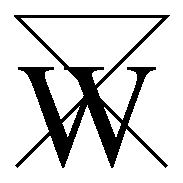
\includegraphics{w.eps}}
\sbox{\boxrosette}{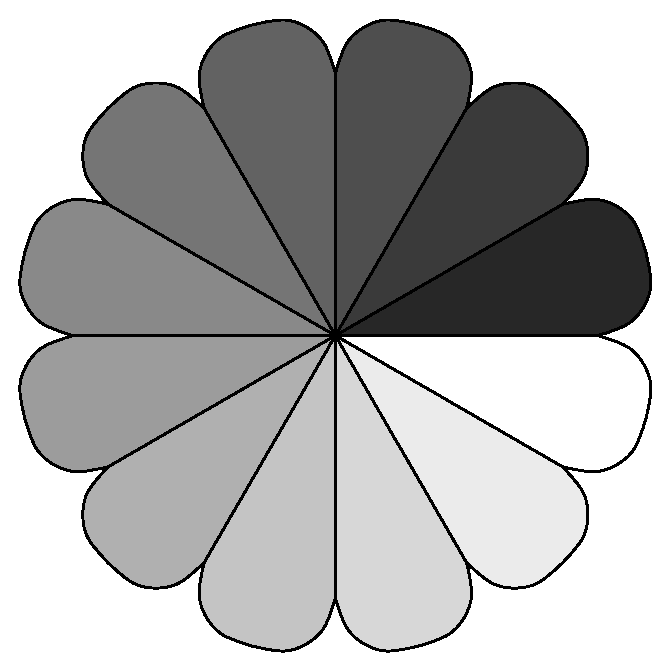
\includegraphics{rosette.eps}}
\sbox{\boxrosettebox}{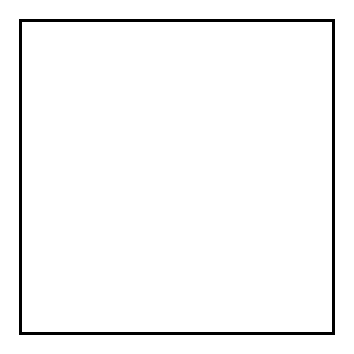
\includegraphics{rosettebox.eps}}

\newenvironment{narrow}[2]{%
	\begin{list}{}{%
			\setlength{\topsep}{0pt}%
			\setlength{\leftmargin}{#1}%
			\setlength{\rightmargin}{#2}%
			\setlength{\listparindent}{\parindent}%
			\setlength{\itemindent}{\parindent}%
			\setlength{\parsep}{\parskip}}%
	\item[]}{\end{list}}
\DeclareCaptionStyle{BigLeft}{style=default, labelsep=period,
	font=Large, labelfont=bf,
	justification=RaggedRight,
	singlelinecheck=false}
\DeclareCaptionFont{BigAndBold}{\Large\bfseries}
\DeclareCaptionLabelFormat{hash}{\bothIfFirst{#1}{ }{\#}#2}
\DeclareCaptionLabelSeparator{arrow}{\quad\ensuremath{\Rightarrow}\quad}
\DeclareCaptionFormat{reverse}{#3#2\ensuremath{\ll}#1\ensuremath{\gg}}
\renewcommand\theContinuedFloat{\alph{ContinuedFloat}}

%% Highlight color definition, from WangLei's epslatex-cn, ver 2000
\definecolor{highlightcolor}{rgb}{1,1,0.8}
\definecolor{mygreen}{rgb}{0,0.5,0}
\definecolor{RoyalBlue}{cmyk}{1,0.50,0,0}
\definecolor{light}{cmyk}{0,0,0,0.50}
\definecolor{morelight}{cmyk}{0,0,0,0.20}
\definecolor{Newlight}{cmyk}{0,0,0,0.20}
\definecolor{SkyBlue}{cmyk}{0.62,0,0.12,0}
\definecolor{NiceColor}{rgb}{0.21,0.42,0.73}
\definecolor{PartColor}{cmyk}{0.12,0.59,0,0}
\definecolor{VerbatimColor}{cmyk}{0.45,0.86,0,0}
\definecolor{PageColor}{rgb}{0.21,0.42,0.73}

\addbibresource{ref.bib}

\makeindex

\begin{document}


\def\HugeRoman{\bfseries\fontsize{2cm}{2cm}\selectfont\color{white}}
\def\HugeChinese{\bfseries\fontsize{1.5cm}{1.5cm}\selectfont\color{light}}

\thispagestyle{empty}
\newpagecolor{PageColor}\afterpage{\restorepagecolor}

\AddToShipoutPicture*{%
    \setlength{\unitlength}{1cm}%
    \color{white}%
    \linethickness{5pt}%
    \put(3,0){\line(0,1){30}}
    \put(0,5){\line(1,0){3}}
    \put(0,10){\line(1,0){3}}
    \put(0,15){\line(1,0){3}}
    \put(0,20){\line(1,0){3}}
    \put(0,25){\line(1,0){3}}
}

%\vspace{10pt}
{\hspace{-15pt}\hypertarget{title}{\HugeRoman \LaTeXe{}}}%
\hfill{%
    \raisebox{-40pt}{%
        \fcolorbox{white}{white}{%
            \parbox{2.5cm}{%
                \vbox to 12cm{%
                    \vfill\hbox to 2.5cm{\hfill\CJKfamily{hei}\HugeChinese 插\hfill}%
                    \vfill\vfill
                    \hbox to 2.5cm{\hfill\CJKfamily{hei}\HugeChinese 图\hfill}%
                    \vfill\vfill
                    \hbox to 2.5cm{\hfill\CJKfamily{hei}\HugeChinese 指\hfill}%
                    \vfill\vfill
                    \hbox to 2.5cm{\hfill\CJKfamily{hei}\HugeChinese 南\hfill}%
                    \vfill}
            }
        }
    }
}

\vskip -7.5cm

\hskip -15pt
\begin{overpic}[scale=0.5]{golfer}
    \put(4,48){\huge \color{red}{\bf \LaTeX}}
    \put(4,38){\huge \color{red}{\bf Graphics}}
    \put(31,7){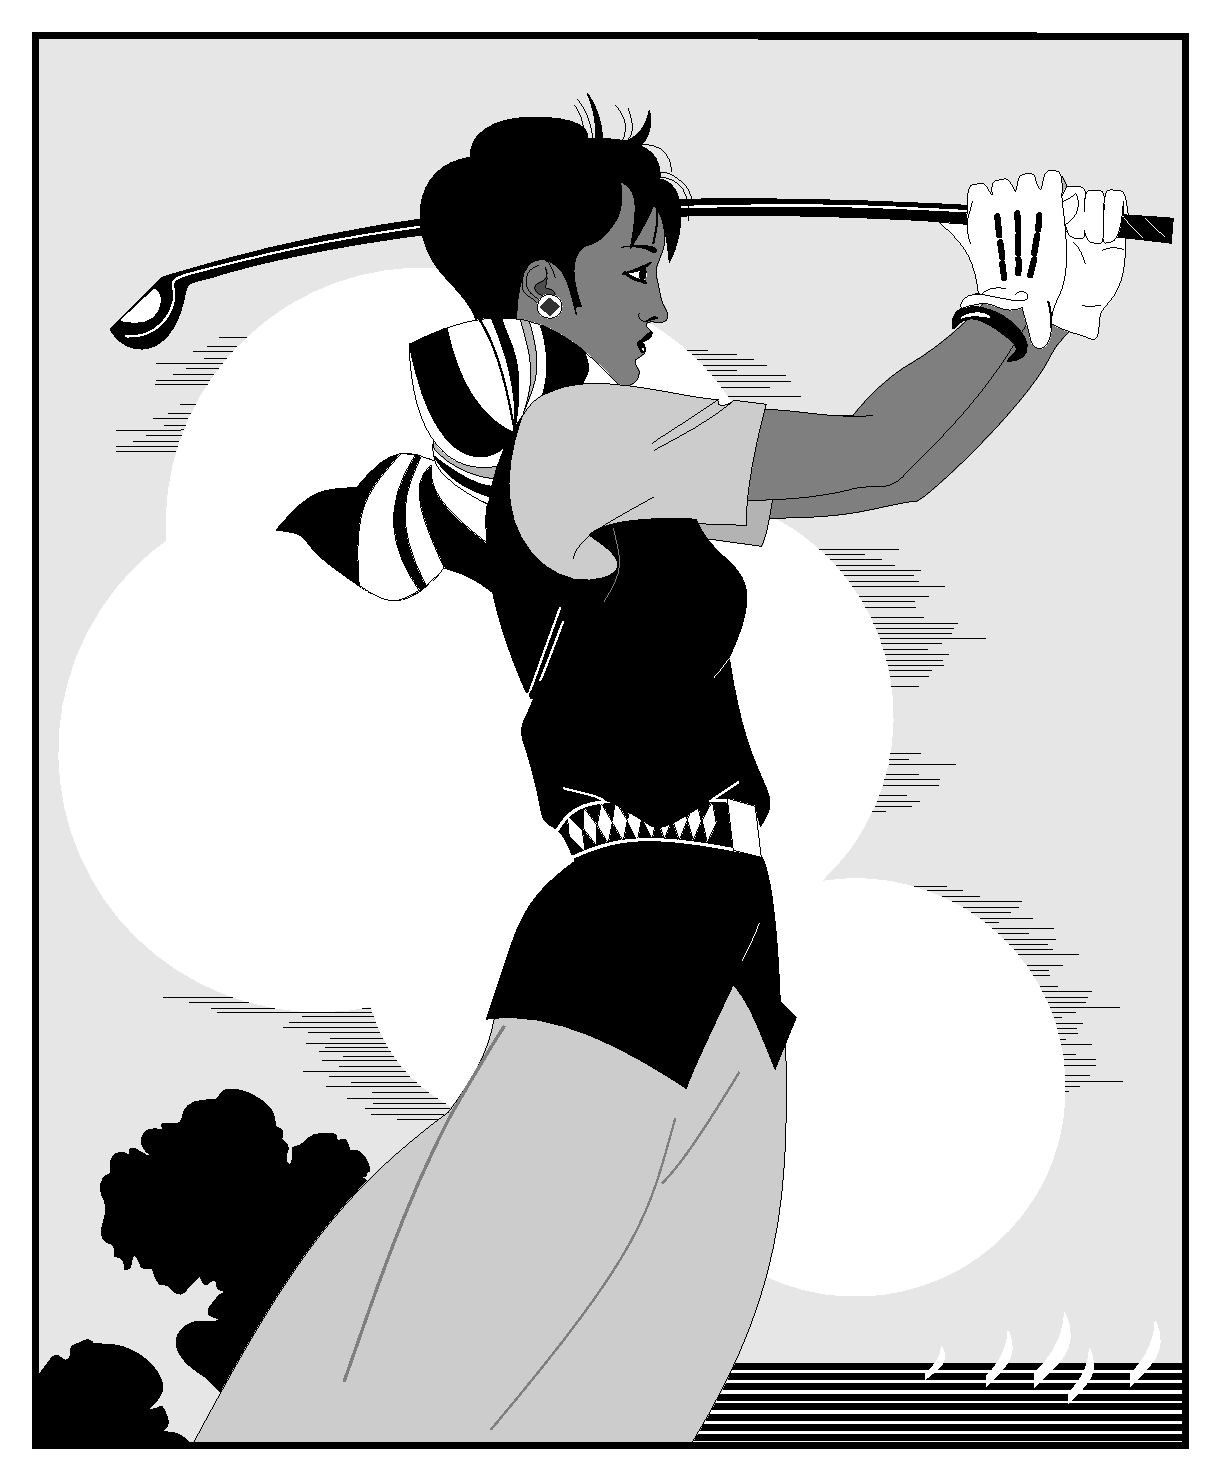
\includegraphics[scale=.25]{golfer}}
    \put(49,11){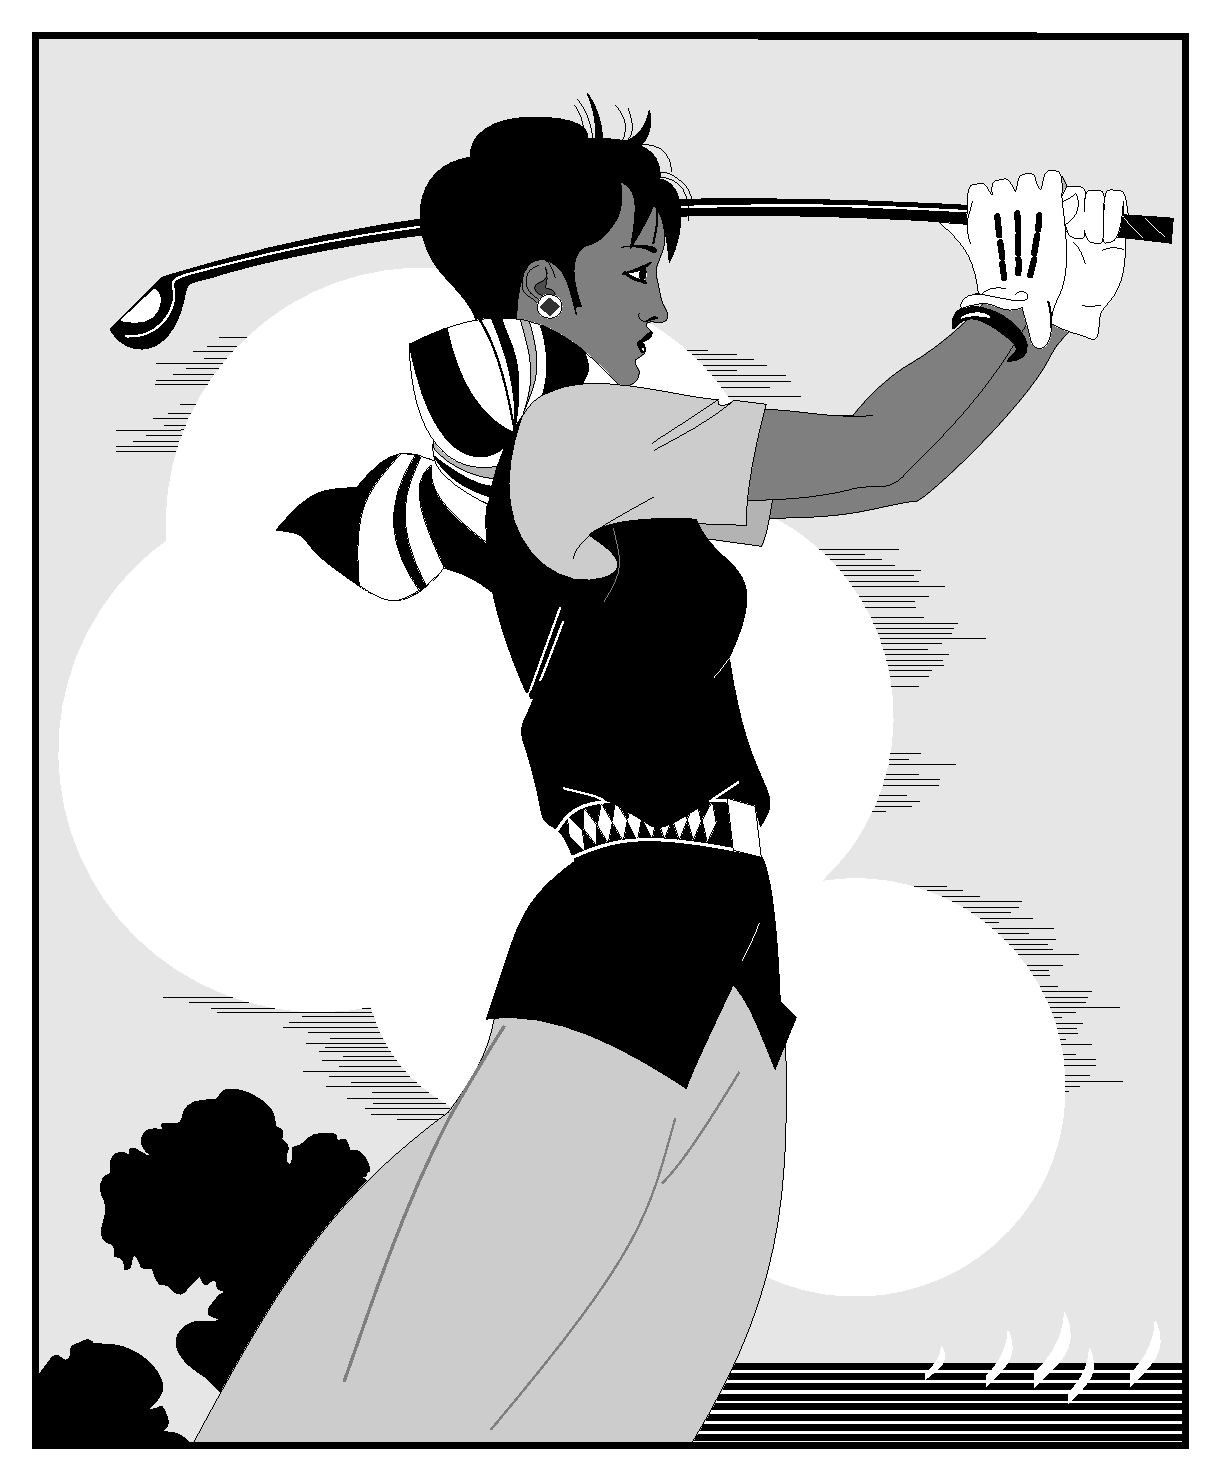
\includegraphics[scale=.10]{golfer}}
\end{overpic}

\clearpage

\thispagestyle{empty}

\begin{center}

\vbox to \textheight{\vfill
{\Large Using Imported graphics in \LaTeX{} and \pdfLaTeX} \\[25pt]
{\large Keith Reckdahl }\\
{epslatex at yahoo dot com}\\[25pt]
Version 3.0.1 \\
January 12, 2006
\vfill}
\end{center}


\clearpage

\setcounter{page}{1}


%preface.tex

\section*{译序}

本文档是Keith Reckdahl所著``Using Imported Graphics in \LaTeX\ and \pdfLaTeX'' 的中文译本。

Keith Reckdahl于1997年原著有文档``Using Imported Graphics in \LaTeXe{}''
(版本2.0,以下简称为 epslatex2),
并且已经由王磊前辈在2000年将其翻译成《\LaTeXe{} 插图指南》。
该译本由于质量上乘,历史悠久,并且作为帮助文档附在CTEX套装内发行,
因此在国内流传甚广、影响力甚大。

然而,也正是因为历史悠久,所以出现了很多与当前 \LaTeX{} 插图技术脱节的地方。
例如只讨论 \prgname{latex}+\prgname{dvips} 模式下 \file{eps} 图像格式的插入,
以及使用 \pkg{caption2} 等过时宏包进行插图标题的处理等等。
为此,原作者在2006年将epslatex2更新为版本3.0.1(以下简称为 epslatex3)。
虽然关于 \LaTeX{} 插图这一话题有不少书籍和电子文档都有相关介绍,
不过即便距今已十年有余,但英文版epslatex3仍可以说是最详尽的参考文档。
而国内除了一些出版的书籍外,尚没有一份全面的专题文档介绍关于插图的各方面知识。
这也正是翻译epslatex3的动机。

随着这些年 \LaTeX{} 的发展,特别是相关宏包以及 \XeTeX{}、\LuaTeX 等新编译引擎的出现和发展,
2006年版本的epslatex3也有不少已经过时的知识。
因此在翻译过程中也加入了译者自己的一些修改。
较大的改动有:
\begin{itemize}
	\item 原文档第7节只讨论了 \prgname{dvips} 和 \prgname{pdftex} 两种引擎程序。
	这里加入了 \prgname{dvipdfmx}、\prgname{xetex}和 \prgname{luatex}等更多编译方式。
	\item 原文档12.1节提到了 \pkg{overpic} 宏包,
	本文档基于旧译本,在第~\ref{ssec:overpic} 节加以详细介绍。
    \item 在第~\ref{sssec:esopic} 节简要介绍了 \pkg{eso-pic} 宏包用法。
	\item 原文档的第32节使用 \pkg{subfig} 宏包处理子图标题,
	这里代之以介绍 \pkg{subcaption} 宏包。
	\item 第~\ref{sec:figintext} 节关于图文混排的内容来自于旧译本。
\end{itemize}
对于明显过时的章节将在行文处加以说明,但出于完整性考虑仍然翻译出来供参考。
此外,行文各处的细节修改则通过脚注的方式给出。

本文档主要是在王磊前辈的译文基础上,
结合英文版epslatex3对epslatex2的变动翻译而来。
考虑到目前的 \LaTeX{} 编译程序并非只有 \pdfTeX{},
因此参照旧译本仍命名为《\LaTeXe{} 插图指南》。
继续使用或修改了旧译本中添加的内容已征得原译者许可。
在翻译过程中还参考了刘海洋的著作《\LaTeX{} 入门》以及其它相关宏包的文档,
在此一并表示感谢。

本文档可在 \LaTeX\ 项目公共协议(LPPL, \LaTeX\ Project Public License)下复制和分发。
LPPL 协议的内容见 \url{http://www.latex-project.org/lppl/}。

\begin{flushright}
盛文博\\
\href{mailto:wbsheng88@foxmail.com}{<wbsheng88@foxmail.com>}\\
二零一七年八月
\end{flushright}

\newpage
\section*{前言}
\label{sect:preface}

在用 \LaTeX\ 编写论文、书稿时,经常要遇到使用图形的情况。
本书将讲述如何在 \LaTeX\ 文件中插入图像以及其它一些相关问题。\footnote{
    原文档涉及到图片的单词包括“figure”和“graphic”,
    前者指的是 \LaTeX{} 文档中作为独立单元的图元素,而后者更偏向于来自于外部的图片文件及图片内容。
    本译文中将 figure 和 graphic 分别翻译为“图形”和“图像”。——译注}
由于完全阅读本书需要较多的时间,
如果想要查询某一特定的信息,
那么可以通过\hyperref[toc]{目录}和\hyperref[sec:index]{索引}直接阅读相关内容。

插图的基本步骤是,首先确认宏包的导入
\begin{lstlisting}
\usepackage{graphicx}
\end{lstlisting}
然后使用 \cmd{includegraphics} 命令来插图
\begin{lstlisting}
\includegraphics{file}
\end{lstlisting}
该命令的更多细节将在第~\ref{sec:graphicsinclusion} 节介绍。

本文档分为如下的五个部分。

\paragraph{第一部分:背景介绍}
这一部分介绍了一些有关的历史资料和基本的 \LaTeX{} 术语。
此外还包括
\begin{itemize}
	\item Encapsulated PostScript (\file{eps}) 图形格式,\file{eps} 与 \file{ps} 文件的区别,
	以及将其它图形格式转为 \file{eps} 格式的方法。
	\item 通过 \pdfTeX 引擎可以直接导入的图片格式(\file{jpeg}, \file{png}, \file{pdf}, \MetaPost)。
	\item 一些与图形有关的自由软件和共享软件。
\end{itemize}

\paragraph{第二部分:\LaTeX{} 图形宏集}
这一部分详细介绍了 \LaTeXe{} 图形宏集中用于导入、缩放和旋转图形的命令。
这部分涵盖了 \LaTeXe{} 图形宏集文档的大部分内容\cite{grfguide}。

\paragraph{第三部分:\LaTeXe{} 图形命令的使用}
这一部分介绍了如何使用 \LaTeXe{} 图形宏包套件中的命令来引入、缩放和旋转图形。
此外还讨论了以下三种情况:
\begin{itemize}
	\item 在支持管道(例如 UNIX )的系统中,使用 \prgname{dvips} 还可以实时地插入压缩的 EPS 图形或其它格式的图形(\file{tiff}, \file{gif}, \file{jpeg}, \file{pict} 等)。
	在其它的系统中,非 \file{eps} 格式图形必须先转换为 \file{eps} 才行。
	因为无论 \LaTeX\ 还是 \prgname{dvips} 都没有内置解压缩和转换图像格式转换的功能,
	所以相应软件需要使用者提供。
	\item 由于许多图形应用程序只支持 \ascii 文本格式,
	\pkg{psfrag} 宏包可以将 \file{eps} 图形中的文字替换为 \LaTeX{} 符号或数学表达式。
	\item 当一个\file{eps}图形被多次使用时(比如文字后面或页眉上的徽标),最后生成的 \file{ps} 文件会包含此\file{eps}图形的很多个副本。
	当所使用的图形不是位图格式时,可以通过定义 PostScript 命令来避免此图形被重复插入,
	从而减小得到的\file{eps}文件体积。
\end{itemize}

\paragraph{第四部分:\env{figure} 环境}
将插入的图形放置于\env{figure} 环境中有几个优点:
在\env{figure}环境中的图形会被自动编号,从而可以引用或添加到目录中;
置于该环境中的图形可以通过浮动实现较好的分页,所以可以很容易制作出具有专业水准的文稿。
除了介绍\env{figure}环境的一般信息外,这一部分还讲述了如下一些和图形有关的话题:
\begin{itemize}
	\item 怎样自定义\env{figure}环境,例如怎样调整图形的位置、图形周围的距离、
	标题的距离,以及在图形与文本之间加入分隔线等。
	还可以自定义标题的格式,改变标题的样式、宽度和字体等。
	\item 怎样创建边注图形和伸入边注位置的宽图形。
	\item 怎样在纵向页面版式的文档中加入横向图形。
	\item 怎样将标题放置于图形的两边而不是上下。
	\item 对于双面排版的文档,怎样确保一幅图形放置于奇数页或偶数页。
	还有,怎样确保两幅图形都出现在同一对开页面上。
	\item 怎样得到带框的图形。
\end{itemize}

\paragraph{第五部分:复杂图形}
这一部分介绍如何创建较为复杂的图形,用以同时包含多个图像。
\begin{itemize}
	\item 怎样形成并列的图形、图像和子图。
	\item 怎样在一个浮动体内将一个表格放置于图形之后。
	\item 怎样堆叠多行图形。
	\item 怎样创建跨页的连续图形。
\end{itemize}

\subsection*{如何得到本文档}
本书的 \file{pdf}格式和 \file{ps}格式的英文原版网络位置为\footnote{
此段有删改。——译注}
\begin{center}
	\href{http://ctan.tug.org/tex-archive/info/epslatex/english/epslatex.pdf}{CTAN/info/epslatex/english/epslatex.pdf}\\
    \href{http://ctan.tug.org/tex-archive/info/epslatex/english/epslatex.ps}{CTAN/info/epslatex/english/epslatex.ps}
\end{center}
本文档版本2.0的法文版本由Jean-Pierre Drucbert完成,
其 \file{pdf} 和 \file{ps} 文件可以从如下位置获得
\begin{center}
    \href{http://ctan.tug.org/tex-archive/info/epslatex/french/fepslatex.pdf}{CTAN/info/epslatex/french/fepslatex.pdf} \\
    \href{http://ctan.tug.org/tex-archive/info/epslatex/french/fepslatex.ps}{CTAN/info/epslatex/french/fepslatex.ps}
\end{center}
完整的 CTAN (Comprehensive \TeX{} Archive Network) 映像站点可以从 \url{https://ctan.org/mirrors} 获得。

\subsection*{致谢}
略。

\subsection*{许可协议}
版权所有 \copyright{} 1995--2006  Keith Reckdahl.
可在 \LaTeX\ 项目公共协议(LPPL, \LaTeX\ Project Public License)下复制和分发。

LPPL 协议的内容可参见 \url{http://www.latex-project.org/lppl/}。


\clearpage
\endinput


\tableofcontents\label{toc}

%part1.tex
\part{背景知识}

\section{简介}\label{sec:introduction}
当高德纳编写 \TeX{} 的时候,还没有 PostScript/\file{eps}、\file{jpeg}、\file{gif} 以及其它图像格式。
\marginpar{历史渊源}
因此 \file{dvi} 文件对于图像导入并没有直接的支持。
不过,\TeX{} 允许\file{dvi} 文件中包含 \cmd{special} 命令,
通过它可以向调用 \file{dvi} 文件的程序传递命令。
因此,凡是调用 \file{dvi} 的程序支持的图像格式,
\TeX\ 和 \LaTeX\ 都能够导入。

过去的许多年来,\file{dvi} 通常都被转为 PostScript 格式,
进而标准的插图格式是 Encapsulated PostScript(\file{eps})图像,
因为它是PostScript语言的一个子集。
在 \LaTeX{} 中插入\file{eps}图像最初通过低层命令 \cmd{special} 来完成。
为了使插图更加方便并且更具有可移植性,
专门为 \LaTeX 2.09 设计了两个高层的宏包 \pkg{epsf} 和 \pkg{psfig}。
\textsf{epsf} 提供了 \cmd{epsfbox} 命令来插入图片,
此外另有三个命令来控制图片的缩放。
在 \pkg{psfig} 中,\cmd{psfig} 命令除了用来插入图片,还有缩放和旋转功能。
不过,尽管 \pkg{psfig} 的句法更受欢迎,它的代码却没有 \pkg{epsf} 健壮。
于是作为这两个宏包的结合的产物,
\pkg{epsfig} 宏包使用 \pkg{psfig} 的句法和大部分 \pkg{epsf} 的健壮代码。
不过,\pkg{epsfig} 仍然使用了一些不健壮的 \pkg{psfig} 代码。

随着 1994 年 \LaTeXe{} 的发布,
\marginpar{\LaTeX{}\\图形宏集}
\LaTeX 3 小组认识到在 \LaTeX{} 插图中存在的一些普遍问题。
通过努力,他们开发出了“\LaTeX\ 图形宏集”,\footnote{
    已经有 \LaTeX{} 图形宏集的 plain \TeX{} 版本,
	相关文件请见 \href{ftp://ctan.tug.org/tex-archive/macros/plain/graphics/}{CTAN/macros/generic/graphics/}}
并全部重写了其中的命令。
比起其它的插图命令,他们的命令更高效、更健壮、更具有可移植性。

\LaTeX{} 图形宏集包括“标准”的 \pkg{graphics} 宏包和“扩展”的 \pkg{graphicx} 宏包。
这两个宏包都有一个 \cmd{includegraphis} 命令,不过版本不同。
类似 \pkg{psfig} 的句法,
\pkg{graphicx} 版的 \cmd{includegraphis} 采用“命名参数(named arguments)”。
这使用起来比较简单方便,却违反了 \LaTeX{} 关于可选参数放置位置的语法指南方针。
作为折中方案,就有了两种版本的 \cmd{includegraphics}。
其中,\pkg{graphics} 的版本遵从 \LaTeX{} 的语法规则,
而\pkg{graphicx} 的版本则采用更为简便的命名参数。
\pkg{graphicx} 版本的 \cmd{includegraphics} 支持图形的缩放和旋转,
而 \pkg{graphics} 版本的 \cmd{includegraphics} 则必须被置于 \cmd{scalebox} 或 \cmd{rotatebox} 才能达到同样的效果。

本文档使用 \pkg{graphicx} 宏包,因为它的句法比 \pkg{graphics} 宏包更加简便易用。
其实这两个宏包具有相同的功能,本文档中的例子同样可以用 \pkg{graphics} 宏包完成,
只不过相应的命令有些笨拙和缺少一点效率。
关于这两个宏包详细的说明可参见 \LaTeX{} 图形宏集的文档~\cite{grfguide}。

出于向后兼容性,\LaTeX\ 图形宏包套件中也提供了一个 \pkg{epsfig} 宏包,
用以替代之前 \LaTeXe\ 的 \pkg{epsfig}。
新的\pkg{epsfig} 定义了 \cmd{epsfbox}、\cmd{psfig} 和 \cmd{epsfig} 等命令。
不过它们只是调用 \cmd{includegraphics} 命令的简单封装。
由于这些封装效率没有直接使用 \cmd{includegraphics} 命令高,
因此,该 \pkg{epsfig} 宏包应当只用于旧文档。
在编写新文档时要用 \cmd{includegraphics}。

除了改进 \file{eps} 图片的部分,
\marginpar{非 \file{eps}\\图形}
\LaTeX{} 图形宏集还处理非 \file{eps} 图像格式的插图问题,
例如\file{jpeg} 和 \file{gif}等。
由于 \file{dvi} 到 \file{ps} 的转换程序一般不直接支持大部分的非\file{eps} 格式,
向 PostScript 文档中插入这些图像之前相关图像必须首先转成 \file{eps} 格式。
尽管这种图像格式的预处理通常是最佳办法,
不过,\LaTeX\ 图形宏集还提供了另一种选择:\file{dvi} 转 \file{ps} 时自动地实时转换图像格式。
第 \ref{ssec:convertor} 节(\pageref{ssec:convertor} 页)介绍了一下图像转换程序,
第 \ref{sec:dvips-noneps} 节(\pageref{sec:dvips-noneps} 页) 讲述了如何在 \file{dvi} 转 \file{ps} 时使用非 \file{eps} 格式的图像。

过去,PostScript 通常是 \LaTeX{} 文档的最终格式,
\marginpar{\pdfTeX}
整个编译过程有两个步骤:
(1) 使用 \LaTeX{} 生成 \file{dvi} 文件,
(2) 使用一个 \file{dvi} 到 \file{ps} 的转换程序(例如\prgname{dvips}) 来生成 PostScript 文件。
之后,随着 Adobe 公司的 \file{pdf} 格式开始流行,编译过程又加了第三步:
(3) 使用 \prgname{Ghostscript}\footnote{
    自由软件,见第 \ref{ssec:gs} 节(\pageref{ssec:gs} 页)。}、
\prgname{Adobe Acrobat}\footnote{
    商业软件,见 \url{www.adobe.com}}
或者 \prgname{PStill}\footnote{
    共享软件,见 \url{www.pstill.com}}
等工具将 PostScript 文件转成 \file{pdf} 文件。

然而,这种三步骤过程 \LaTeX-\prgname{dvips}-\prgname{ghostscript} 不仅很繁琐,
而且很难实现一些 \file{pdf} 特性,比如超链接。
为了改进这一点,\HanTheThanh{} 写了一个工具叫做 \TeX2PDF,
这一工具修改了 \TeX\ 引擎,可以直接从 \TeX{} 生成 \file{pdf}。
\TeX2PDF 最终重命名为 \pdfTeX,
并且在许多志愿者的帮助下(托高德纳的福)进行扩展,
进而实现了 \TeX{} 的全部排版功能。
\pdfTeX 从名称上看来输出的是 \file{pdf},
不过它也能输出 \file{dvi} 格式,并且与原先 \TeX{} 引擎的输出结果相同。

如同 \prgname{latex} 命令使用 \TeX{} 引擎处理 \LaTeX{} 文档并生成 \file{dvi} 文件,\footnote{
现代的 \TeX 发行版本中,\prgname{latex} 命令使用的也是 \pdfTeX{} 引擎。——译注}
\prgname{pdflatex} 命令使用 \pdfTeX{} 引擎处理 \LaTeX{} 文档,并直接生成 \file{pdf} 文件。
 
\pdfTeX{} 的一个重要特性就是原生支持许多图像格式:
\marginpar{\pdfTeX{} 和图像}
\file{jpeg}、\file{png}、\file{pdf}、\MetaPost。
尽管老版本的 \pdfTeX{} 还支持 \file{tiff} 文件,目前的 \pdfTeX{} 版本不支持 \file{tiff}。

另外要注意的是,\pdfTeX{} 不能直接导入 \file{eps} 文件\footnote{
    \pdfTeX{} 可以导入由 \prgname{PurifyEPS} 处理的 \file{eps} 文件,
	见第 \ref{ssec:purifyeps} 节(\pageref{ssec:purifyeps} 页)。},
用户需要用 \prgname{epstopdf} 等程序将 \file{eps} 文件转成 \file{pdf} 格式,
不过这样就不能直接使用 \pkg{PSfrag} 宏包(见第 \ref{ssec:psfrag} 节,\pageref{ssec:psfrag} 页)。

目前\footnote{
    此段由译者添加},
\marginpar{其它编译引擎}
除了 \prgname{latex}+\prgname{dvips} 和 \prgname{pdflatex} 之外,
还有几种常见的编译方式:
\begin{description}
	\item \prgname{dvipdfmx} 可以从 \file{dvi} 文件生成 \file{pdf} 文件。
	\item \prgname{xelatex} 可以直接生成 \file{pdf} 文件。支持UTF-8编码和使用各种字体。
	\item \prgname{lualatex} 作为 \prgname{pdflatex} 的后继引擎,引入了Lua动态编程语言。
	可以直接生成 \file{pdf} 文件。支持UTF-8编码和使用各种字体。
\end{description}
出于技术上的先进性、稳定性以及效率和兼容性考虑,
一般而言推荐使用 \prgname{xelatex} 编译方式。
特别是对于中文文档,这样可以直接使用系统字体,避免了繁琐的中文配置过程。
而对于英文文档,也可以考虑使用 \prgname{pdflatex}。

以上几种编译方式都原生支持 \file{eps}、\file{pdf}、\file{jpg}、\file{png} 等各种图片格式。
不过这样就不能直接使用 \pkg{PSfrag} 宏包(见第 \ref{ssec:psfrag} 节,\pageref{ssec:psfrag} 页),
因为该宏包要求输出格式是 PostScript。


\section{\LaTeX{} 术语}\label{sec:terminology}

任何 \LaTeX{} 对象(字符,图形等)都把\emphi{盒子}作为单位 \cite[103页]{Lamport1994}。
每个盒子在它的左侧均有一个\emphi{参考点}(\emphi{Reference point})。
盒子的\emphi{基线}(\emphi{baseline},见图~\ref{fig:samplebox})是一条通过参考点的水平线。
当 \LaTeX{} 从左到右排列文本时,
每一字符的参考点排成一条水平直线,称为\emphi{当前基线}(\emphi{current baseline}),
并使它与字符的基线对齐。
\LaTeX{} 也用同样的方法来处理图形和其它对象,每个对象的参考点都被放置于当前基线上。

\begin{figure}
	\centering
	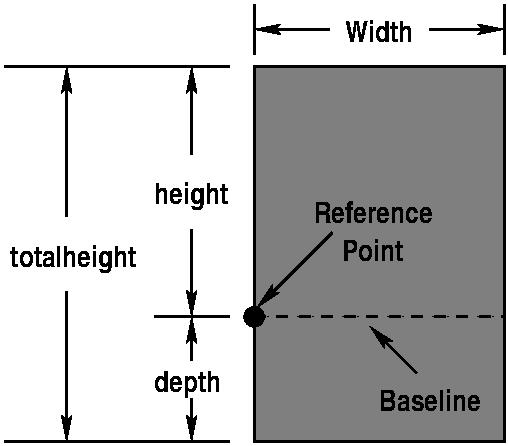
\includegraphics[width=.4\linewidth]{latex-box}
	\caption{\LaTeX{}~盒子示例}
	\label{fig:samplebox}
\end{figure}

每一个盒子的大小由三个长度决定:
\emphi{高度}(\emphi{height})、\emphi{深度}(\emphi{depth})和\emphi{宽度}(\emphi{width})。
高度是参考点到盒子顶部的距离,深度是参考点到盒子底部的距离,宽度则是盒子的宽度。
而\emphi{整体高度}(\emphi{totalheight})定义为盒子底部到顶部的距离,
即:$\text{\emph{整体高度}} = \text{\emph{高度}} + \text{\emph{深度}}$。

未旋转图形的参考点是它的左下角(见图~\ref{fig:rotate-box} 左边的盒子),它的深度为零,高度就等于全部高度。
图~\ref{fig:rotate-box} 中间的盒子则是将图形旋转后,它的高度就不等于全部高度了。
右边的盒子则展示可将图形旋转使其高度为零。

\begin{figure}
	\centering
	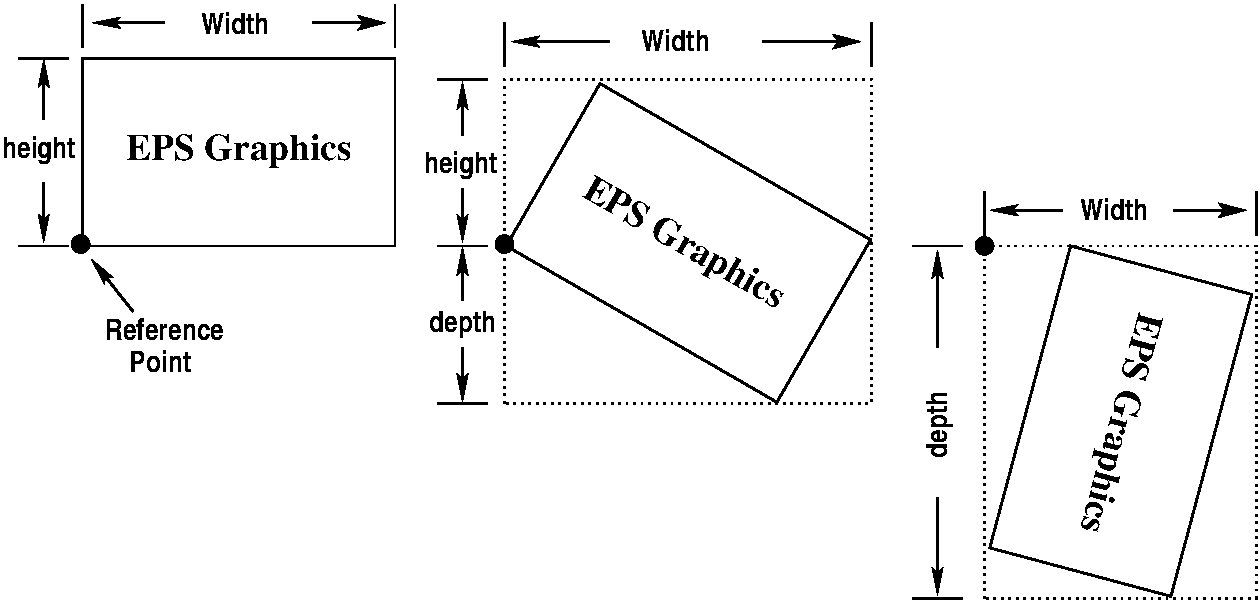
\includegraphics[width=.9\linewidth]{rotat-box}
	\caption{\LaTeX{}~盒子的旋转示例}\label{fig:rotate-box}
\end{figure}

\section{Encapsulated PostScript}\label{sec:eps}

PostScript 语言能够用来描述图形和文本。
它既可在传统的PostScript (\file{ps})文件中来描述多页文档,也用于 Encapsulated PostScript  (\file{eps})文件中来描述插入文档的图像。
\file{ps} 文件和 \file{eps} 文件的主要区别在于:
\begin{itemize}
	\item \file{eps} 文件只能使用部分特定的 PostScript 操作符。
	\item \file{eps} 文件必须含有一个 BoundingBox 行来确定 \file{eps} 图像的大小。
\end{itemize}


\subsection{禁止使用的 PostScript 操作符}\label{ssec:forbidps}

由于 \file{eps} 图形需要和其它对象一起共享页面,
所以 \file{eps} 文件中不能使用页面操作,
例如选择页面大小(\texttt{a4} 或 \texttt{letter})和清除整个页面(\texttt{erasepage})等命令。
下面是不能在 \file{eps} 文件中使用的 PostScript 操作符:

\begin{center}
\ttfamily
\begin{tabular}{lllll}
	a3   &  a4 &  a5 &   banddevice & clear  \\
	cleardictstack & copypage &  erasepage & exitserver & framedevice \\
	grestoreall & initclip & initgraphics & initmatrix & letter  \\
	legal & note & prenderbands & quit & renderbands \\
	setdevice & setglobal & setpagedevice & setpageparams & setsccbatch \\
	setshared & startjob & stop & & \\
\end{tabular}
\end{center}

尽管下列 PostScript 操作符可以在 \file{eps} 文件中使用,
但是不适当地使用它们极易导致错误。
\begin{center}
\ttfamily
\begin{tabular}{llll}
	nulldevice & setcolortransfer & setgstate & sethalftone \\
	setmatrix & setscreen & settransfer & undefinedfont \\
\end{tabular}
\end{center}

上面的一些操作符可能会使\file{dvi} 到 \file{ps} 的转换失败,
另一些则可能导致像图像位置错误、消失或者闪烁等奇怪的问题。
因为这些操作符绝大部分不会影响到PostScript的堆栈,
所以在大多数情况下,简单地将这些招致问题的操作符删除就可解决问题。
其它的情形则需要更为复杂的PostScipt编程知识。

\subsection{EPS BoundingBox}\label{ssec:bbox}
\index{EPS BoundingBox}

习惯上,PostScript 文件的第一行标明了该文件的PostScript类型,
接下来的几行是被称为 \emph{header} 或\emph{preamble} 的注释行(PostScript 的注释符也是 \texttt{\%})。
其中一行定义了 BoundingBox,包括四个整数值,分别代表:
\begin{enumerate}
	\item BoundingBox 的左下角的 $x$ 坐标。
	\item BoundingBox 的左下角的 $y$ 坐标。
	\item BoundingBox 的右上角的 $x$ 坐标。
	\item BoundingBox 的右上角的 $y$ 坐标。
\end{enumerate}

例如,一个由 \prgname{gnuplot} 程序生成的 \file{eps} 文件的前五行为

\begin{lstlisting}[language=PostScript]
%!PS-Adobe-2.0 EPSF-2.0
%%Creator: gnuplot
%%DocumentFonts: Times-Roman
%%BoundingBox: 50 50 410 302
%%EndComments
\end{lstlisting}

这个\prgname{gnuplot} 生成的 \file{eps} 图像的左下角的坐标是 $(50,50)$,
右上角的坐标是 $(410,302)$。
这里坐标的单位是PostScript 点,一点等于 $\nicefrac{1}{72}$ 英寸。
这样上面的这幅图的自然宽度为 $5$ 英寸,相应的自然高度为 $3.5$ 英寸。
需要注意的是PostScript 点要比 \TeX{} 点(等于 $\nicefrac{1}{72.27}$ 英寸)稍大。
在 \TeX{} 和 \LaTeX{} 中,PostScript 点被称为“大点”(``big points'')或简称 \texttt{bp},
而 \TeX{} 点被称为``points''或简称 \texttt{pt}。

\subsection{将PS转换为EPS}\label{ssec:pstoeps}

单页的PostScript文件,如果没有包含不适当的命令的话,
可用下述方法之一加上BoundingBox行并转为\file{eps}文件。
\textbf{由于这些方法都不检查非法的PostScript操作符,
	所以只有在被转换的PostScript文件本身不含有那些被禁制使用的操作符的情况下,才能得到正确的\file{eps} 文件。}

\begin{enumerate}
	\item 最方便的是用GhostScript里带的\prgname{ps2epsi}工具(见第~\ref{ssec:gs} 节,\pageref{ssec:gs} 页)。
	它可以读入PostScript文件,计算 BoundingBox 的参数,
	然后生成一个含有PostScript 图像的\file{eps} 文件。
	
	最终得到的 \file{eps} 文件是 \file{epsi} 格式,
	即它在文件的开始部分带有一个低分辨率的Interchange预览位图。
	因为这个预览位图是 \ascii 编码的,
	所以不会造成像第 \ref{ssec:linebuffer} 节的 \texttt{bufsize} 错误。
	不过,\file{epsi} 预览会增加文件体积。\index{bufsize@\texttt{bufsize}}
	\item 另外一种通过 Ghostscript 计算 BoundingBox 参数的方法是使用 \prgname{epstool} 工具。
	该程序适用于Unix、DOS、Windows和OS/2系统,获取链接为
	\begin{center}
		\url{http://www.cs.wisc.edu/~ghost/gsview/epstool.htm}
	\end{center}
	例如,如下命令
\begin{verbatim}
    epstool --copy --bbox file1.eps file2.eps
\end{verbatim}
	分析 \file{file1.eps} 的内容来决定正确的 BoundingBox,
	然后将带有计算后的BoundingBox值的 \file{file1.eps} 内容复制给 \file{file2.eps}。
	\prgname{epstool} 工具还可以用于在 \file{eps} 文件内添加 \file{tiff}、\file{wmf} 以及 \file{epsi} 预览位图,
	或者用于从 \file{eps} 文件中提取预览位图。
	
	\item 此外,还有一种办法是,计算 BoundingBox 的参数,
	然后把它加到PostScript文件中或作为插图命令的参数
	(比如用 \cmd{includegraphics} 的 \texttt{bb} 选项)。
	计算BoundingBox 参数的方法有以下几种:	
	\begin{enumerate}
		\item 用 Ghostview 或 GSview 将 PostScript 图形打开。
		当鼠标在图形上移动时就会显示相应的坐标(以页面的左下角为参照点)。
		记下图形的左下角和右上角的坐标就可确定它的 BoundingBox。
		\item 将 PostScript 图形打印一份,
		测量页面的左下角到图像的左下角的水平和竖直距离(以英寸为单位),
		然后乘以 $72$ 就可以得到 BoundingBox 的左下角坐标。
		类似地,测量页面左下角到图像右上角的水平和竖直距离就可以得到 BoundingBox 的右上角坐标。
		\item \pkg{bbfig} 脚本使用 PostScript 打印机来计算 BoundingBox。
		\pkg{bbfig} 会在PostScript文件开头添加一些 PostScript 命令并送往PostScript打印机。
		在打印机处,添加的PostScript命令会计算 BoundingBox坐标,
		然后将结果打印在PostScript图像上面。
		\pkg{bbfig} 脚本程序的地址为
		\begin{center}
			\href{ftp://ctan.tug.org/tex-archive/support/bbfig/}{CTAN/support/bbfig/}
		\end{center}		
	\end{enumerate}
\end{enumerate}

\subsection{修正非标准的EPS文件}\label{ssec:fixeps}
一些应用程序(例如 \prgname{Mathematica} 和 \prgname{FrameMaker} )会生成非标准的 \file{eps} 文件,
不能在\LaTeX\ 等其它程序上使用。
有一些应用程序会根据它们自己的偏好给 PostScript 加入了额外特性,
还有一些应用程序生成非常糟糕的 PostScript 代码。
通常来说,这些非标准的PostScript可以由软件公司自己或者精通PostScript的用户提供的脚本来修正。
检索软件供应商的网页或者搜索相关软件的网络新闻组来获取相关信息。

\section{\LaTeX{} 怎样使用 EPS 图}\label{sec:useeps}

当处理\prgname{dvips} 类型文件时,\LaTeX{} 和 \file{dvi} 到 \file{ps} 的转换程序都会使用 \file{eps} 文件。
\begin{enumerate}
	\item \LaTeX{} 通过读取 \file{eps} 文件中的BoundingBox行来决定为 \file{eps} 图形保留多大的空间。
	\item \file{dvi} 到\file{ps}的转换程序读取\file{eps}文件并把它插入到生成的\file{ps} 文件中。
\end{enumerate}

需要说明的几种情形:
\begin{itemize}
	\item 如果在插图命令中给定了BoundingBox的值
	(例如,使用了 \cmd{includegraphics} 的 \opt{bb} 选项),
	\LaTeX{} 将不会再读取 \file{eps} 文件。
	事实上,当运行 \LaTeX{} 时,\file{eps} 文件甚至都不必存在。
	\item 由于 \TeX{} 不能读取非 \ascii 文件,也不能生成其它的程序,
	所以 \LaTeX{} 不能从压缩的 \file{eps} 文件或其它非 \file{eps} 图像文件中得到BoundingBox的信息。
	在这种情况下,BoundingBox参数值必须由插图命令给定(例如 \cmd{includegraphics} 命令的 \opt{bb} 选项)
	或者存放在一个未压缩的文本文件中(见第~\ref{sec:dvips-noneps} 节,\pageref{sec:dvips-noneps} 页)。
	\item \file{eps} 图像并没有包含在\file{dvi}文件中。
	当 \file{dvi} 转换为 \file{ps} 时,\file{eps} 文件必须存在。
	因此,所有用到的\file{eps}文件必须和 \file{dvi} 文件放在一起。
	\item 一些 \file{dvi} 浏览器可能不支持显示 \file{eps} 图像。
	这时,为了方便使用者对图像进行定位,一般会将图形的BoundingBox用一个方框显示出来。
\end{itemize}

\subsection{行缓冲区溢出}\label{ssec:linebuffer}

\TeX{} 在读取 \ascii 文件时是每次从中读取一行,然后把它放到自己的行缓冲区里。
\TeX{} 的行缓冲区大约有3000个字符长度。
如果 \file{eps} 文件中有一行的长度超过了行缓冲区的长度,就会产生如下的错误讯息:

\begin{Verbatim}[xleftmargin=22pt]
	Unable to read an entire line--bufsize=3000.
	Please ask a wizard to enlarge me.
\end{Verbatim}

因为\file{eps}很少有一行长度超过3000个字符的情形,
所以产生行缓冲区溢出错误的原因可能有两种:

\begin{enumerate}
	\item \textbf{ EPS 文件中有一个长的二进制预览图}

	有些应用程序生成的\file{eps} 文件在开始部分放置了一个二进制的预览图,
	这样就可使得像\file{dvi} 浏览器等一些不能解释PostScript的软件也可来显示 \file{eps} 图形。
	目前有少数与\TeX{} 有关的软件使用这种方法。
	
	如果这个二进制预览图比行缓冲区小,\cmd{includegraphics} 将会略过它\footnote{
        注意,\cmd{psfig} 和其它一些过时的图像命令则不会忽略二进制预览。}。
	但是,如果这个二进制的预览图比行缓冲区大的话,就会发生行缓冲区溢出的错误。
	对于该问题有两种解决办法:
	
	\begin{enumerate}
		\item 如果不需要预览图,可以用文本编辑器将它删掉或在一开始用应用程序生成\file{eps} 图像时就选择不要预览图。
		\item 因为 \LaTeX{} 读取 \file{eps} 文件的唯一目的就是取得BoundingBox参数值大小,
		因此,如果插图命令中给出BoundingBox的值(如在 \cmd{includegraphics} 中使用 \opt{bb} 选项),
		那么\LaTeX{} 就不会读取 \file{eps} 文件。
	\end{enumerate}
	
	\item \textbf{\file{eps} 文件中的分行符在不适当的传输中被损坏}
	
	\emph{这里所谈到的问题不会在大部分最近的\TeX{} 发行版本中出现,
		因为这些软件中的\TeX{} 程序都会正确的识别所有的分行符。}
	
	不同的操作系统平台使用不同分行符。
	Unix 使用换行符LF(\verb+^J+),
	Macintosh 使用回车符CR( \verb+^M+),
	而 DOS/Windows 则使用回车符加换行符( \verb+^M^J+)。
	比如一个\file{eps} 文件从 Macintosh机上用二进制方式传输到Unix机上,
	那么Unix机上的\TeX{} 会因找不到分行符 \verb+^J+ 而把整个文件作为一行,导致行缓冲区溢出的错误。
	
	如果\file{eps} 文件中不含有二进制的部分(如预览图和嵌入的图形),
	以文本方式传输就可以解决这一问题。
	然而,带有二进制部分的 \file{eps} 文件必须用二进制方式传输,
	否则文本方式传输会损坏二进制部分。
	由于二进制传输方式不会翻译分行符,这时就需要在插图命令中给出BoundingBox的值来解决
	(例如 \cmd{includegraphics} 命令的 \opt{bb} 选项)。
\end{enumerate}

\section{PDF 图像}\label{sec:pdfgraphics}
正如之前提到的,\pdfTeX{} 可以直接导入 \file{pdf}、\file{png}、\file{jpeg} 和 \MetaPost{} 图像格式。
这一节将简要介绍这些格式。
相关的\pdfTeX{} 插图命令将在第~\ref{sec:graphicsinclusion} 节(\pageref{sec:graphicsinclusion} 页)中介绍。

\subsection{JPEG}\label{ssec:jpeg}
\file{jpeg} 是由联合图像专家组(Joint Photographic Experts Group , JPEG)委员会
\begin{center}
	\url{http://www.jpeg.org/}
\end{center}
授权的压缩标准。
\file{jpeg} 格式是一种位图的压缩标准,它采用了有损压缩格式\footnote{
    有损压缩意味着压缩过程中损失了数据。
	也就是说,解压缩一个有损压缩过的位图不会得到原始图片。
	反之,无损压缩过程中不会有数据损失,
	所以解压一个无损压缩过的位图会生成原始图片。}。
特别地,压缩过程不会保持线条和锋锐的边缘。
所以不太适用于线条描绘和带有锋锐元素的图片。

\subsection{PNG}\label{ssec:png}
过去很多年 \file{gif} 一直是图标和其它线条画的位图压缩标准,
这是由于它采用的无损LZW压缩不会使得锋锐的边缘失真。
由于Unisys公司对于其LZW专利的强制执行,加上\file{gif} 的一些技术局限(例如256色的限制),
这些因素促使了一个小组开发可移植网络图形( Portable Network Graphics , PNG )格式。
该小组后来称为 \file{png} 开发组
\begin{center}
\url{http://www.libpng.org/pub/png/}
\end{center}
与 GIF 一样,PNG也采用无损压缩,因此适合于线条画。
尽管 \file{png} 可以用于任何位图文件,
不过对于摄影照片和其它一些没有锋锐边缘的位图来说,
\file{jpeg} 有损压缩通常效果更好( “更好”指的是生成更小的文件体积,同时对于人眼观察没有失真)。

\subsection{PDF}\label{ssec:pdf}
\href{http://www.adobe.com}{Adobe} 的便携式文档格式( Portable Document Format, \file{pdf} )与它的Adobe成员 PostScript 有很多相似之处。
与PostScript一样,\file{pdf} 可以包含文本、矢量图和位图。
一个 \file{pdf} 文件可以包含整个文档,也可以仅仅包含一个图形(类似于 \file{eps} )。

\file{pdf} 不仅仅是 \pdfTeX{} 的主要输出格式,也是 \pdfTeX{} 插图的最普遍方法。
许多图像程序允许它们的图像直接保存为 \file{pdf} 格式。
没有直接 \file{pdf} 输出的程序可以转而输出 \file{eps} 矢量图,
后者通过 \prgname{epstopdf} 转换程序可以很容易地转成 \file{pdf} 矢量图。
\prgname{epstopdf} 可以从 \textsc{ctan} 获得,
在Windows系统下是一个可执行程序,在Unix/Linux 以及 MaxOSX 等其它系统上则是一个\prgname{perl} 脚本
\begin{center}
\href{ftp://ctan.tug.org/tex-archive/support/epstopdf/}{CTAN/support/epstopdf/}
\end{center}

\subsection{\MetaPost}\label{ssec:metapost}
\MetaPost{} 是由John Hobby编写的绘图语言。
它基于高德纳的 \MetaFont ,但增加了PostScript输出的功能。
关于 \MetaPost{} 的信息可以从以下网址获得:
\begin{center}
\url{http://www.tug.org/metapost.html}
\end{center}
相关文档可参考~\cite{metapost-doc}。

\MetaPost 可以用于 \prgname{dvips} 类型的 \LaTeX{} 文档,
也可以直接用于 \pdfLaTeX{} 文档\footnote{
	\pdfLaTeX{} 实际上使用Hans Hagen开发的 {Con\TeX t} 代码将 \MetaPost{} 图像实时转成 \file{pdf},
	不过在用户层面上是很简明的。}。

下面的步骤使用 \MetaPost( \prgname{mpost} )所带的 \prgname{pstoedit} 工具将名为 \file{graphic.eps} 的 \file{eps} 文件转为名为 \file{graphic.mps} 的 \MetaPost{} 文件:

\begin{verbatim}
	pstoedit -f mpost graphic.eps graphic.mp
	mpost graphic.mp
	rename graphic.1 graphic.mps
\end{verbatim}

\subsection{PurifyEPS}\label{ssec:purifyeps}
Scott Pakin 的 \prgname{purifyeps} 工具能够将很多(但不是全部) \file{eps} 转成“净化版本”,
从而可以直接被 \LaTeX{} 和 \pdfLaTeX{} 读取。
为了运行 \prgname{purifyeps} 你需要下列工具:
\begin{description}
	\item[PurifyEPS] 可以从\href{ftp://ctan.tug.org/tex-archive/support/purifyeps/}{CTAN/support/purifyeps/} 获得。
	\item[Perl] 可以从 \url{http://www.cpan.org} 获得。
	\item[pstoedit] 可以从 \url{http://www.pstoedit.net/pstoedit} 获得。
	\item[mpost] 来自于任何包含 \MetaPost{} 的\LaTeX{} 发行版本。
\end{description}


\section{图像软件}\label{sec:graphicsoftware}
[{\bfseries 本节介绍的部分软件可能已经过时,仅供参考。——译注}]
\subsection{Ghostscript}\label{ssec:gs}
Ghostscript 是一个 PostScript/\file{pdf} 解释器,
它可以运行在大多数操作系统平台上,并且是自由发布的\footnote{
	尽管 AFPL Ghostscript (之前叫做 Aladdin Ghostscript )是免费发布的,
	但却不是公有领域。
	它受版权保护,有一些限制,例如不允许商业发布等。
	当 Aladdin Ghostscript 的版本停止了大约一年之后,
	Aladdin 将其以“GNU Ghostscript”发布,使用的是限制性不那么强的 GNU Public License。}。
通过 Ghostscript,PostScript、\file{eps} 和 \file{pdf} 文件可以在屏幕显示,
也可以用 Postscript 和 非 PostScript 打印机来打印。
AFPL Ghostscript 可以从 Ghostscript 官网获得:
\begin{center}
	\url{http://ghostscript.com/}
\end{center}
其中包含了预编译的Windows、DOS、OS/2 和 Macintosh 可执行文件,
以及在 Unix/VMS 下可用的源代码。
此外还有一些Ghostscript的图形界面软件,例如GSview、Ghostview、GV等,
可以更方便地浏览 PostScript。

Ghostscript中还带有一些有用的工具,如 \prgname{ps2pdf} 等,可利用Ghostscript来
转换图形,打印、预览 PostScript文件。
详细的使用说明可参考Ghostscript所带的使用说明文件。

\subsection{图像格式转换工具}\label{ssec:convertor}

下面列出的一些免费软件和共享软件可以用来转换图像格式。
在 \prgname{dvips} 模式文件中,这些程序可以将非\file{eps} 图像转成 \file{eps}。
在 \pdfLaTeX{} 文档中,这些程序可以将图像转成可以支持的格式( \file{pdf}、\file{png}、\file{jpeg} )。
其中一些程序还提供命令行方式,这样就可以实时转换图像,
具体见第~\pageref{ssec:noneps} 页的~\ref{ssec:noneps} 节

\begin{description}
	\item[ImageMagick] 
	
	\prgname{ImageMagick} 是一个开放源代码的自由软件,
	适用于创建、编辑和合并位图图片。
	它可以读取、转换和写入各种格式的图片。
	可以进行的操作包括:剪裁图片,修改颜色或是应用各种效果,旋转和合并图片,
	添加、拉伸和旋转文字、线条、多边形、椭圆和贝塞尔曲线。
	
	例如,当 \prgname{ImageMagick} 的 \prgname{convert} 命令添加到系统的环境变量后,
	如下命令会将 \file{file.jpg} 存为 \file{eps} 版本。
\begin{verbatim}
		convert file.jpg file.eps
\end{verbatim}
	
	使用通配符可以批量转换文件,例如
\begin{verbatim}
		convert *.gif image.png
\end{verbatim}
	会将当前路径下的所有 \file{gif} 文件转为 \file{png} 版本,并保存为
\begin{verbatim}
		images-0.png
		images-1.png
		...
\end{verbatim}
	想要将 \file{png} 文件名保存成原始的 \file{gif} 文件名则比较复杂,
	需要写一个 shell 脚本或者 Windows 批处理文件。
	
	\prgname{ImageMagick} 可以运行在所有主流的操作系统上。
	可执行程序和相关信息可以从下面的网址下载
	\begin{center}
		\url{http://www.imagemagick.org/}
	\end{center}
	
	\item[GraphicsMagick]
	\prgname{ImageMagick} 的接口不时发生变化,
	这会导致调用 \prgname{ImageMagick} 的代码发生不兼容性。
	作为 \prgname{ImageMagick} 5.2.2 的一个分支,
	\prgname{GraphisMagick} 项目于2002年11月开始开发,
	旨在提供一套具有稳定接口的图像转换工具,
	它的侧重点在于修复bugs而不是添加新特性。
	
	\prgname{GraphicsMagick} 可以在 Unix/Linux、Cygwin、MacOSX和Windows系统上运行。
	可执行程序和源代码可以从如下网址下载
	\begin{center}
		\url{http://www.graphicsmagick.org/}
	\end{center}
	
	\item[NetPBM]
	\prgname{NetPBM} 是现在已经不维护的 \prgname{PBMPLUS} 程序包的自由开源版本。
	\prgname{NetPBM} 是一个关于图像操作的工具箱,
	包括在各种类型的格式之间相互转换。
	该程序包内有超过220种不同的工具,可以在约100种图像格式之间转换。
	\prgname{NetPBM} 使用命令行操作,没有图形界面。
	
	大部分的Linux发行版和Cygwin项目都包含 \prgname{NetPBM}。
	Windows、MacOSX和其他操作系统上的 \prgname{NetPBM} 程序可以从下面的网址下载
	\begin{center}
		\url{http://netpbm.sourceforge.net/}
	\end{center}
	
	\item[Irfanview]
	
	\prgname{Irfanview} 是Windows上一款出色的图像软件,
	具有易于安装、简洁、快速等特点。
	\prgname{Irfanview} 支持各种文件格式的浏览和转换,
	并提供基本的图片编辑功能,包括裁剪、重采样、颜色和亮度的调整等。
	\prgname{Irfanview} 同时支持GUI图形界面和命令行操作,包括批处理模式。
	
	例如,当\prgname{Irfanview} 的可执行程序 \verb|i_view32.exe| 添加到Windows的环境变量后,
	如下命令
\begin{verbatim}
		i_view32 *.gif /convert=*.png
\end{verbatim}
	会为当前目录下所有的 \file{gif} 文件创建 \file{png} 版本,
	保存的文件名为原 \file{gif} 文件的文件名加上 \file{.png} 后缀。
	\prgname{Irfanview} 可以从下面的网址下载
	\begin{center}
		\url{http://www.irfanview.com/}
	\end{center}
	\prgname{Irfanview} 对于个人、学术和非盈利用户是免费的,
	商业用户则要求注册费。
	
	\item[Graphic Converter]
	
	Graphic Converter 是一个Macintosh上的共享软件,
	可以读取约190种图片格式,并输出约75种格式。
	更多信息可见
	\begin{center}
		\url{http://www.lemkesoft.de/}
	\end{center}
	
	\item[WMF2EPS]
	
	\prgname{WMF2EPS} 是运行在Windows上的共享软件,
	实现可以 \file{wmf} 到 \file{eps} 的转换。
	获取网址为
	\begin{center}
		\href{http://www.ctan.org/tex-archive/support/wmf2eps}{CTAN/support/wmf2eps/}
	\end{center}
	
	\item[KVEC]
	
	\prgname{KVEC} 是一款自由软件,
	能将 \file{bmp}、\file{gif}、\file{tiff} 等位图格式转化为 PostScript和其它的矢量图格式。
	\prgname{KVEC} 可以运行在 Windows、OS/2、Linux、Unix、Macintosh和BeOS等系统上。
	更多信息可见
	\begin{center}
		\url{http://www.kvec.de}
	\end{center}
	
	\item[xv]
	
	\prgname{xv} 是一个交互式图片操作程序,运行在 X Window 系统下。
	尽管有图像转换的功能,但是 \prgname{xv} 的设计目标是图片操作程序,
	因此不适用于图像转换。
	例如,它没有提供命令行功能,所以图像转换必须一个一个做。
	
	\prgname{xv} 对于非商业使用是共享软件,对于商业使用则要求注册。
	更多信息可见
	\begin{center}
		\url{http://www.trilon.com/xv/xv.html}
	\end{center}
	
	\item[GIMP]	
	
	\prgname{GIMP},即 GNU Image Manipulation Program,是一个图片操作的自由软件。
	它基本上提供了 \prgname{PhotoShop}  的功能。
	\prgname{GIMP} 可以运行在 Unix/Linux、Windows和MacOS上。
	更多信息可见
	\begin{center}
		\url{http://www.gimp.org/}
	\end{center}

\end{description}


\subsection{Level 2 EPS 封装}\label{ssec:epswrapper}
Level 2 PostScript 支持若干种压缩格式,
包括用于 \file{jpeg} 文件的 DCT 和用于许多 \file{tiff} 文件的 LZW。
此外,二进制数据可以是 \ascii 编码的,
比如 \ascii85 或者 \ascii Hex,这样生成的\ascii 文件大小分别是原来二进制文件的$125\percent$ 和 $200\percent$。
由于Level-2 \file{eps}支持这些压缩格式,
因此可以创建为 \file{jpeg} 或是 \file{tiff} 文件的封装。
这样生成的 \file{eps} 比起传统的\file{eps}转换来说具有更高的质量和更小的体积。
如果你有一台 Level 2 PostScript打印机,
那么你最好是用下面的这些封装程序来替代上节中的那些转换软件。
不过由于这样得到的PostScript文件只能在 Level 2 PostScript打印机上打印,会降低文件的通用性。

请注意,默认情况下,\prgname{dvips} 会剥离使用的 \file{eps} 图像的注释行
(即以 \texttt{\%\%} 开头的行)。
由于\ascii85编码的 Level 2 图像会包含以 \texttt{\%\%} 开头的行,
所以,使用 \ascii85编码的 level-2 \file{eps} 文件的用户必须使用\verb|dvips -K0| 选项(\texttt{K} 加上数字 \texttt{0} ),
以阻止 \prgname{dvips} 剥离注释行。
不过,\ascii Hex 编码的 level-2 文件则不会有这个问题。

\begin{description}
	\item[jpeg2ps] 
	
	\prgname{jpeg2ps} 是一个用 C 语言编写的程序,
	可将\file{jpeg} 图像转换为 Level 2 PostScript。
	\prgname{jpeg2ps} 可在 Unix、DOS 和其它操作系统下使用。
	\prgname{jpeg2ps} 可以从如下网址获得
	\begin{center}
		\href{http://www.ctan.org/tex-archive/support/jpeg2ps}{CTAN/support/jpeg2ps/}\\
		\url{http://gnuwin32.sourceforge.net/packages/jpeg2ps.htm}
	\end{center}
	
	\prgname{jpeg2ps} 支持三种 level-2 编码:
	\ascii85 (默认值)、8-bit binary (使用 \verb|jpeg2ps -b| 选项)、7-bit \ascii Hex (使用 \verb|jpeg2ps -h| 选项)。

	\item[tiff2ps]
	
	\prgname{tiff2ps} 可以运行在 Unix、DOS、Mac 和 VMS 系统上。
	\file{tiff} 图像可用\prgname{tiff2ps} 程序转换为 LZW--编码的 Level 2 PostScript。
	\texttt{tiff2ps} 的源代码可以从如下站点获得
	\begin{center}
		\url{http://www-mipl.jpl.nasa.gov/~ndr/tiff/html/tools.html}\\
		\url{ftp://ftp.sgi.com/graphics/tiff/}
	\end{center}
	
	\item[ImageMagick 的 level-2 EPS 功能]
	
	正如第~\pageref{ssec:convertor} 页的~\ref{ssec:convertor} 节所述,
	\prgname{ImageMagick} 可以在一大类图像格式之间转换。
	其中一种格式就是 level-2 \file{eps},
	因此,\prgname{ImageMagick} 具有和上述 level-2 封装相同的功能。
	例如,
\begin{verbatim}
		convert file.jpeg file.eps2
\end{verbatim}
	会为 \file{file.jpeg} 创建一个 level-2 \file{eps} 版本 \file{file.eps2}
	
\end{description}

\subsection{编辑 PostScript}\label{ssec:editps}

虽然可直接编辑 \file{eps} 文件中的PostScript命令来改变图像,
但这对大多数人来说还是很困难的。
所幸的是,借助于下面的一些工具软件,可以很容易地编辑 \file{eps} 图像。

\begin{description}
	\item[pstoedit]
	
	\prgname{pstoedit} 是 Unix、Windows、DOS 和 OS/2 下的自由软件,
	它能够将PostScript或PDF图像转为其它矢量格式
	(比如\file{Xfig} 的 \file{.fig}格式)。
	更多信息可参考
	\begin{center}
		\url{http://www.pstoedit.com/}
	\end{center}

	\item[Mayura Draw]
	
	\prgname{Mayura Draw} 以前称为\prgname{PageDraw},
	是 Windows3.1/95/NT 下的共享软件。
	当与ghostscript一起使用时,它可以编辑PostScript文件。见:
	\begin{center}
		\url{http://www.mayura.com/}
	\end{center}
	
	\item[xfig]
	
	\prgname{xfig} 是 Unix/Xwindows 下功能强大的自由绘图软件,
	能够导入 \file{eps} 图形并加上标记。不过目前还不能改变原始的\file{eps} 图像。
	参见
	\begin{center}
		\url{http://www.xfig.org/}
	\end{center}
	
\end{description}

\clearpage
\endinput


%part2.tex
\part{\LaTeX{}图形宏集}\label{part:graphicbundle}

这一部分简要介绍 \LaTeX{} 图形宏集。
更多细节可以参考图形宏集文档 \cite{grfguide} 或者 \emph{\LaTeX{} Graphics Companion}\cite{Goossens1997}。

\section{图像文件加载}\label{sec:graphicsinclusion}

导入图像需要使用 \pkg{graphicx} 宏包的 \cmd{includegraphics} 命令,语法为
\begin{lstlisting}[frame=shadowbox]
\includegraphics[选项]{文件}
\end{lstlisting}
这里\emph{选项} 在表~\ref{tab:opt}、\ref{tab:cropopt}、\ref{tab:boolopt} 中列出。
因为 \cmd{includegraphics} 不会结束当前段落,所以它能够在文本中放置图形如
 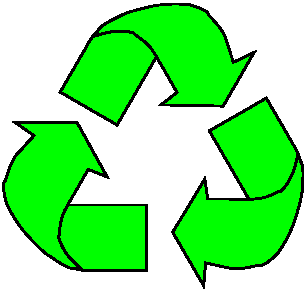
\includegraphics[width=12pt]{recycle} 和 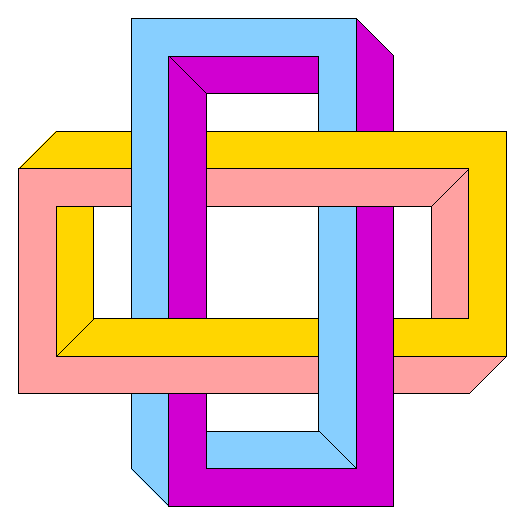
\includegraphics[width=12pt]{illusion}。

\subsection{图形驱动}\label{ssec:driver}
用户必须指定一个图形驱动以告诉图形宏包如何处理导入的图像。
目前\LaTeX{} 图形宏集支持18种不同的驱动
\footnote{
	到目前(2016年)为止,支持的驱动数已经超过了20种。——译注},
不过,本文档只涉及几种最常用的驱动:
\prgname{dvips}、\prgname{dvipdfmx}、\prgname{pdftex}、\prgname{xetex}、\prgname{luatex}。
除了 \prgname{dvipdfmx} 之外,余下几种驱动一般不用显式指明,
因为绝大部分 \LaTeX{} 发行版中的 \file{graphics.cfg} 可以自动识别\footnote{
    \file{graphics.cfg} 文件会检测文件的编译方式。
	对于 \prgname{latex} 会指定 \opt{dvips} 选项,
	对于 \prgname{pdflatex} 会指定 \opt{pdftex} 选项,
	对于 \prgname{xelatex} 会指定 \opt{xetex} 选项,
	对于 \prgname{lualatex} 会指定 \opt{luatex} 选项。
	而对于 \prgname{latex}+\prgname{dvipdfmx} 编译方式,则需要手动声明 \opt{dvipdfmx} 选项,
	因为经由 \prgname{latex} 生成 \file{dvi} 文件后,
	\file{graphics.cfg} 会假定接下来使用 \prgname{dvips}。}。

如果用户想要指定一个驱动,可以用以下三种方式
\marginpar{指定驱动}
\begin{enumerate}
	\item 默认值在 \file{graphics.cfg} 文件中指定。
	\item 任何通过 \cmd{documentclass} 的选项指定的驱动会覆盖由 \file{graphics.cfg} 文件指定的驱动。
	\item 任何由 \cmdM{usepackage}{graphics} 的选项指定的驱动会覆盖前两种方式指定的驱动。
\end{enumerate}

\subsection{DVIPS 模式下图像加载}
\prgname{dvips} 模式下支持最好的图像格式是 \file{eps}。
当使用 \prgname{latex} 编译文件时,下面的命令
\begin{lstlisting}
\includegraphics{file.eps}
\end{lstlisting}
会从 \file{file.eps} 文件中按照自然大小导入图像。
如果文件名没有扩展名,
\begin{lstlisting}
\includegraphics{file}
\end{lstlisting}
那么 \cmd{includegraphics} 会按照 \cmd{DeclareGraphicsExtensions} 扩展名列表中自动加上扩展名
(见~\pageref{ssec:deextension} 的第~\ref{ssec:deextension} 节)。

\subsection[pdfLaTeX 模式下的图像加载]{\pdfLaTeX{} 模式下的图像加载}
\pdfTeX{} 支持直接导入 \file{pdf}、\file{png}、\file{jpeg} 和 \MetaPost{} 图像。
当使用 \prgname{pdflatex} 编译时,下面的命令
\begin{lstlisting}
\includegraphics{file.pdf}
\includegraphics{file.png}
\includegraphics{file.jpg}
\includegraphics{file.mps}
\end{lstlisting}
会按照自然尺寸大小导入 \file{pdf} 文件 \file{file.pdf}、
\file{png} 文件 \file{file.png}、
\file{jpeg} 文件 \file{file.jpg}
以及 \MetaPost{} 文件 \file{file.mps}。
如果文件名没有扩展名
\begin{lstlisting}
\includegraphics{file}
\end{lstlisting}
那么 \cmd{includegraphics} 会按照 \cmd{DeclareGraphicsExtensions} 扩展名列表中自动加上扩展名
(见~\pageref{ssec:deextension} 的第~\ref{ssec:deextension} 节)。

\subsection{同时供 \LaTeX{} 和 \pdfLaTeX{} 编译的文档 }\label{ssec:latexandpdflatex}
很多情况下要求文档同时可以由 \LaTeX{} 或 \pdfLaTeX{} 编译。
要求 PostScript 输出时使用 \LaTeX{} 编译和 \prgname{dvips} 驱动,
要求 \file{pdf} 输出时则使用 \pdfLaTeX{} 编译。
在这两种方式之间切换会改变两件事情。\footnote{
    使用 \prgname{xelatex} 或者 \prgname{lualatex} 编译时无需考虑此问题。
	这是因为这两种编译方式能同时支持 \file{eps} 和 \file{pdf}、\file{jpg}、\file{png} 等图片格式,
	同时编译时也能够自动调用相应的 \pkg{graphicx} 驱动选项。——译注}
\begin{itemize}
	\item 合适的 \pkg{graphicx} 驱动会改变。
	\item 可以直接导入的图像类型会改变。
\end{itemize}
使用如下步骤会调整这些,这样一份文档可以同时由 \LaTeX{} 和 \pdfLaTeX{} 编译。
\begin{enumerate}
	\item 对于每一份要导入的图像都创建两个副本\footnote{
		有时使用 \prgname{PurifyEPS} (见 \pageref{ssec:purifyeps} 页的第~\ref{ssec:purifyeps} 节) 可以创建一个文件并可以同时供 \LaTeX{} 和 \pdfLaTeX{} 使用。}:
	\begin{enumerate}
		\item 一份 \file{eps} 版本,当使用 \prgname{latex} 编译时会导入。
		\item 一份 \file{png}、\file{pdf}、\file{jpeg} 或者 \MetaPost{} 版本,
		当使用 \prgname{pdflatex} 编译时会导入\footnote{
			也可以使用 \prgname{epstopdf} 进行实时转换,
			见下面的第~\ref{sssec:epstopdf} 节。——译注}。
	\end{enumerate}
	
	\item 不要在 \cmd{documentclass} 或者 \cmdM{usepackage}{graphicx} 命令中指定 \opt{dvips} 或者 \opt{pdftex} 选项。
	\file{graphic.cfg} 文件会自动传递合适的选项给 \pkg{graphicx} 宏包。
	
	\item 当使用 \cmd{includegraphics} 命令插图时,
	不要指定扩展名。例如
\begin{lstlisting}
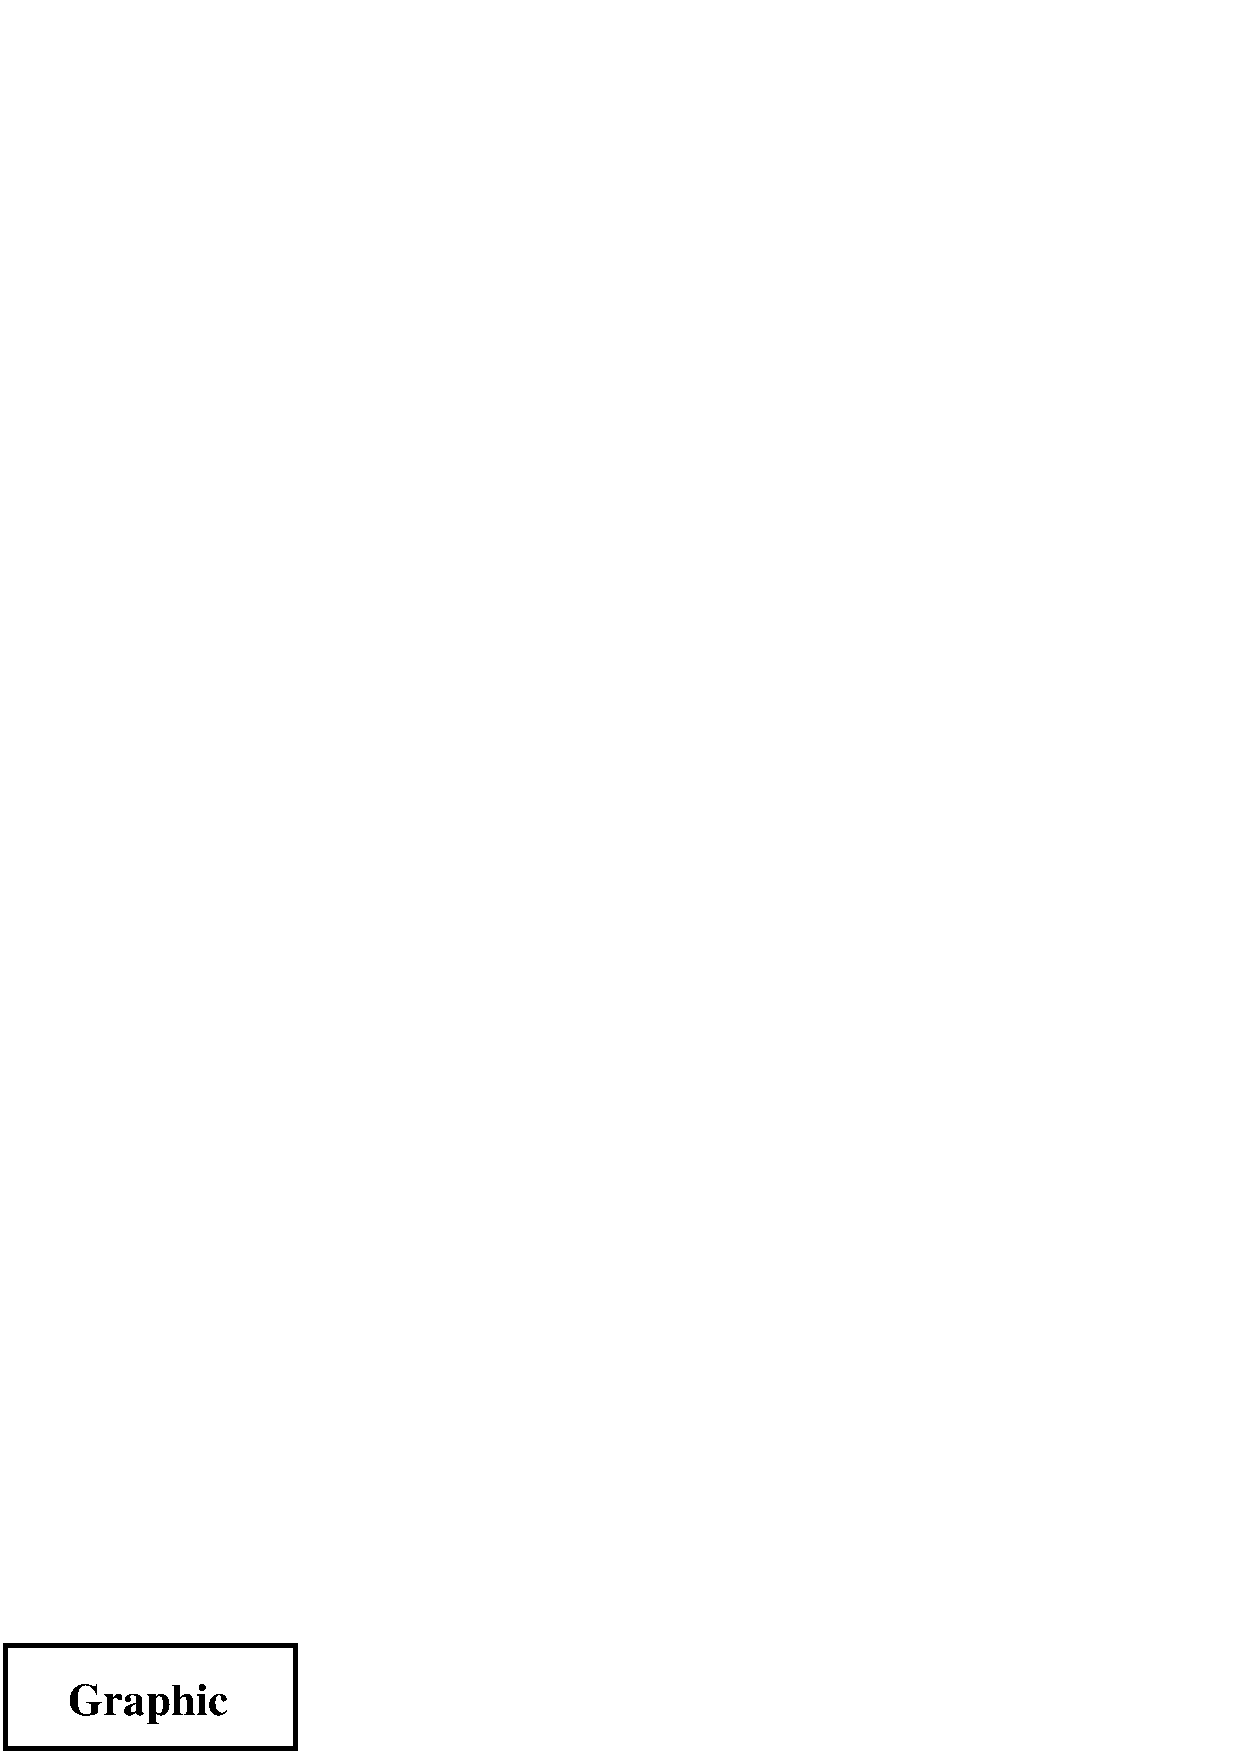
\includegraphics{graphic}
\end{lstlisting}
	定义在 \file{dvips.def} 中的默认扩展名列表会使得 \LaTeX{} 导入图像 \file{eps} 版本,
	而定义在 \file{pdftex.def} 中的默认扩展名列表会使得 \pdfLaTeX{} 导入图像的 \file{png}、\file{pdf}、\file{jpeg} 或者 \MetaPost{} 版本
	(见~\pageref{ssec:deextension} 的第~\ref{ssec:deextension} 节)。
	
	\item 不要直接使用 \pkg{psfrag}。如果需要进行 \pkg{psfrag} 替换,
	使用~\pageref{sssec:psfrag-pdftex} 页的第~\ref{sssec:psfrag-pdftex} 节介绍的方法。
\end{enumerate}

\subsubsection{使用 \pkg{ifpdf} 宏包的条件代码}
\pkgi{ifpdf} 宏包的 \cmdi{ifpdf} 命令会检测文档是否由 \prgname{pdflatex} 编译\footnote{
	历史上,有一种检测方法是基于 \cmd{pdfoutput} 仅在使用 \pdfLaTeX{} 时才有定义这一事实。
	然而,现在绝大部分 \TeX{} 发行版中的 \prgname{latex} 命令实际上是在 \file{dvi} 模式下执行 \pdfLaTeX{}。
	此时无论用\prgname{latex} 和 \prgname{pdflatex} 中的哪种来编译,\cmd{pdfoutput} 都有定义。
	\pkg{ifpdf} 宏包则提供了一个鲁棒的条件命令,可以判断文档是否直接处理成 \file{pdf} 文件,
	从而解决了这一问题。},
进而可以在文档中使用条件语句。

例如,为了精简扩展名列表(见第~\ref{ssec:deextension} 节),
可以用 \cmd{ifpdf} 命令来定制
\begin{lstlisting}
\usepackage{ifpdf}
...
\ifpdf
\DeclareGraphicsExtensions{.pdf,.png,.jpg,.mps}
\else
\DeclareGraphicsExtensions{.eps}
\fi
\end{lstlisting}

如果用户想要基于条件代码来使用不同的 \cmd{documentclass} 选项,
使用如下代码可以在 \cmd{documentclass} 之前定义 \cmd{ifpdf}
\begin{lstlisting}
\RequirePackage{ifpdf}
\ifpdf
\documentclass[pdftex]{article}
\else
\documentclass[dvips]{article}
\fi
\end{lstlisting}
这段代码当使用 \prgname{pdflatex} 时会传递 \opt{pdftex} 选项,
而使用 \prgname{latex} 编译时会传递 \opt{dvips} 选项。
不过,正如~\pageref{ssec:driver} 页的第~\ref{ssec:driver} 节所述,
这段代码实际上没有必要,因为绝大部分的发行版本会根据 \file{graphics.cfg} 文件自动处理驱动选项。

\subsubsection{使用 epstopdf 宏包}\label{sssec:epstopdf}
如果已经准备了 \file{eps} 图像而想使用 \prgname{pdflatex} 编译方式,
可以考虑使用宏包 \pkgi{epstopdf}。
该宏包可以在编译时实时地将 \file{eps} 转成 \file{pdf} 格式图像,
从而可以在 \prgname{pdflatex} 编译方式下使用。\footnote{
    在 \TeX Live (2010之后的较新版本)中会自动调用该宏包,也就是说,此时可以直接用 \prgname{pdflatex} 编译 \file{eps} 插图的情况——译注}

使用该宏包要注意两点:
\begin{itemize}
	\item 需要开启 \cmd{write18} 特性,从而使得可以在编译时调用外部程序。
	具体来说,编译方式为
\begin{lstlisting}[language=bash,escapechar=\%]
pdflatex -shell-escape test.tex %(\TeX Live 中)%
pdflatex -enable-write18 test.tex %(MiK\TeX{} 中)%
\end{lstlisting}
	\item 在图形宏包 \pkg{graphics}/\pkg{graphicx} 之后载入 \pkg{epstopdf},即
\begin{lstlisting}
\usepackage{graphicx}
\usepackage{epstopdf}
\end{lstlisting}
\end{itemize}

结合之前介绍的 \pkg{ifpdf},可以使用如下代码
\begin{lstlisting}
\usepackage{graphicx}
\usepackage{ifpdf}
\ifpdf
\usepackage{epstopdf}
\fi
\end{lstlisting}
这样,在只准备 \file{eps} 格式图像的情况下,
\prgname{dvips} 和 \prgname{pdflatex} 都可以处理文档。

\subsection{指定宽度、高度和角度}\label{ssec:spec-width-height-angle}
如下命令
\marginpar{指定宽度}
\begin{lstlisting}
\includegraphics[width=3in]{file}
\end{lstlisting}
导入指定的图片文件,且宽度为 3英寸\footnote{
    同时高度也会按相应的比例缩放——译注}。
不过,为了使图像的页面布局更具通用性,
图片宽度最好指定为可伸缩的相对长度而不是用像3英寸这样的固定尺寸\footnote{
	预先定义的相对长度包括:\\
	\cmd{textwidth} 是文档中正文的宽度;\\
	\cmd{linewidth} 是当前环境中一行的宽度;\\
	\texttt{em} 是当前字体大写字母M的宽度;\\
	\texttt{ex} 是当前字体小写字母x的高度。}。
例如,
\begin{itemize}
	\item 如下命令将插入的图片伸缩至和当前一行文本的宽度相同:
\begin{lstlisting}
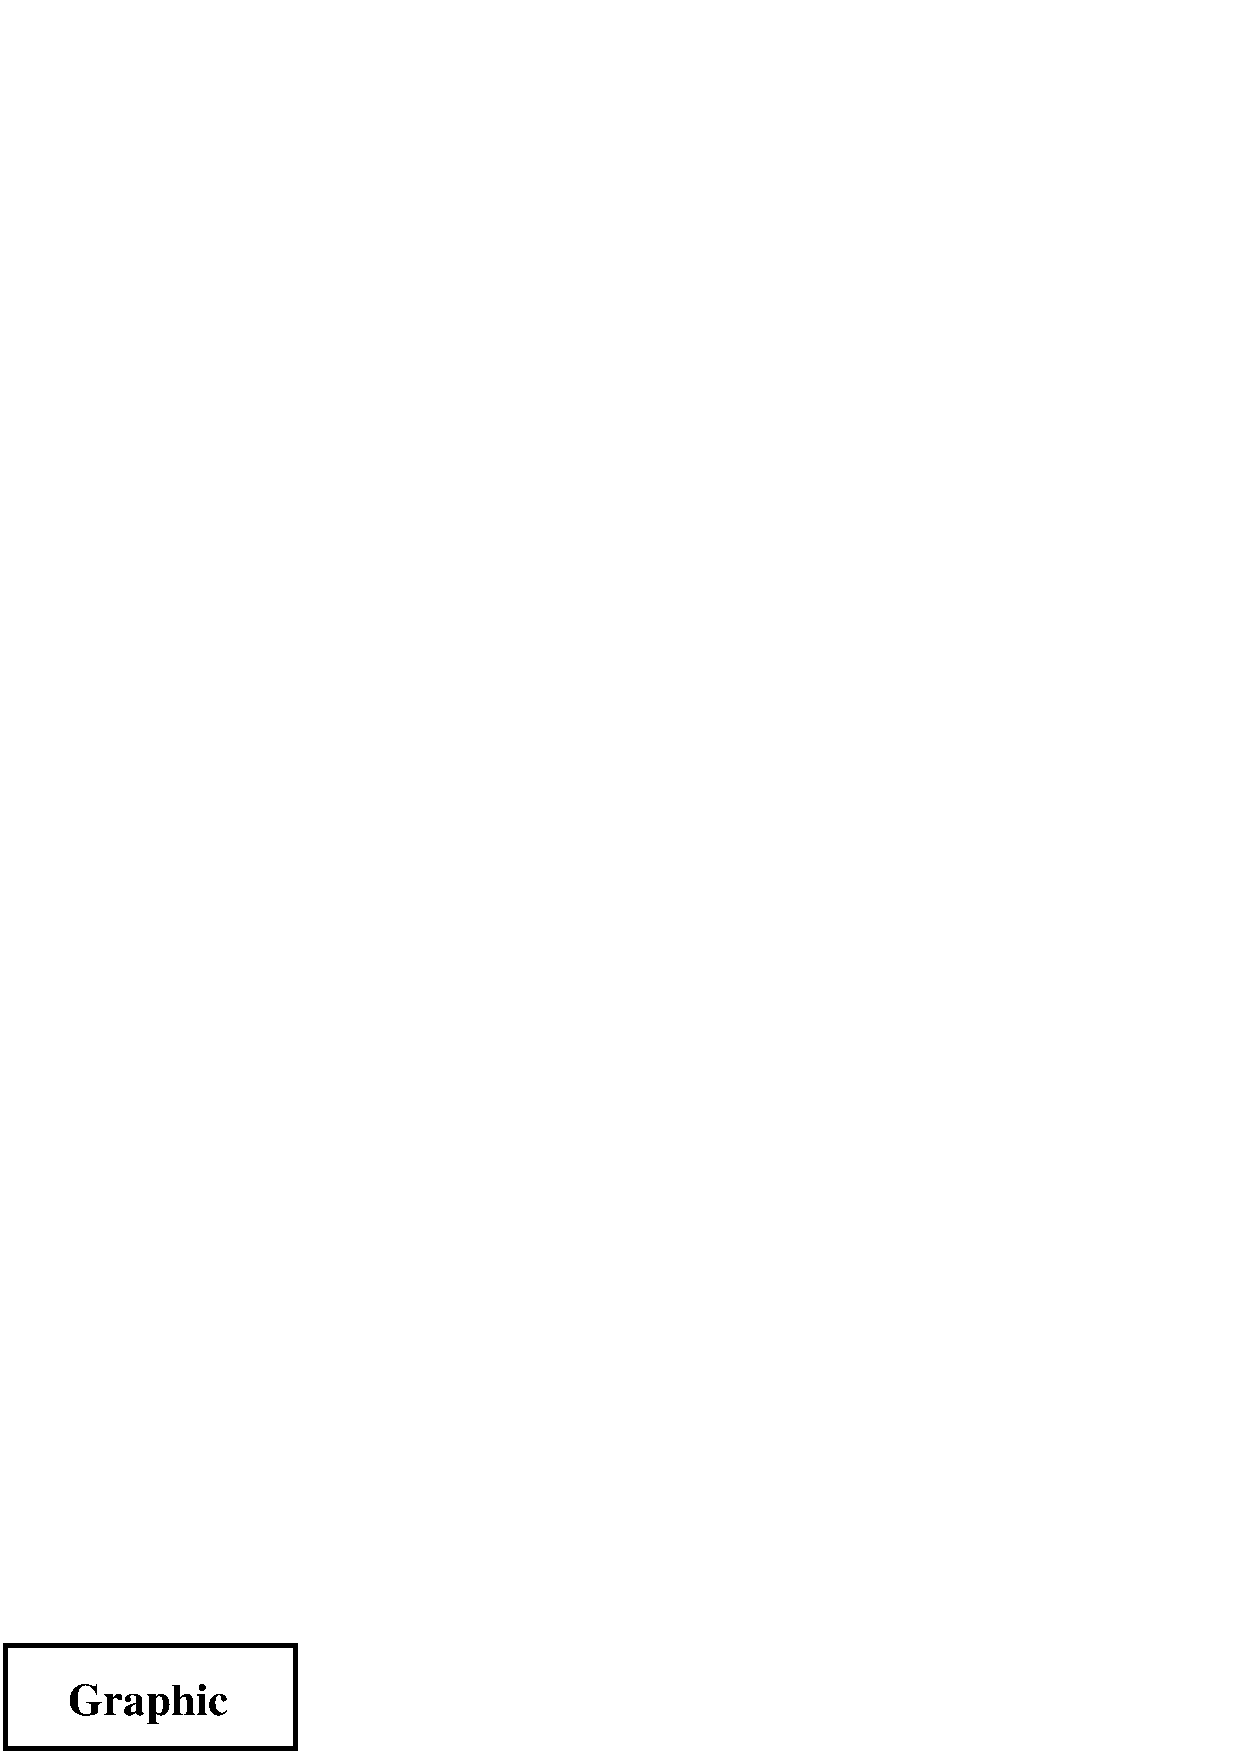
\includegraphics[width=\linewidth]{graphic}
\end{lstlisting}
	\item 如下命令使得插入图片的宽度为当前一行文本的 $80\percent$:
\begin{lstlisting}
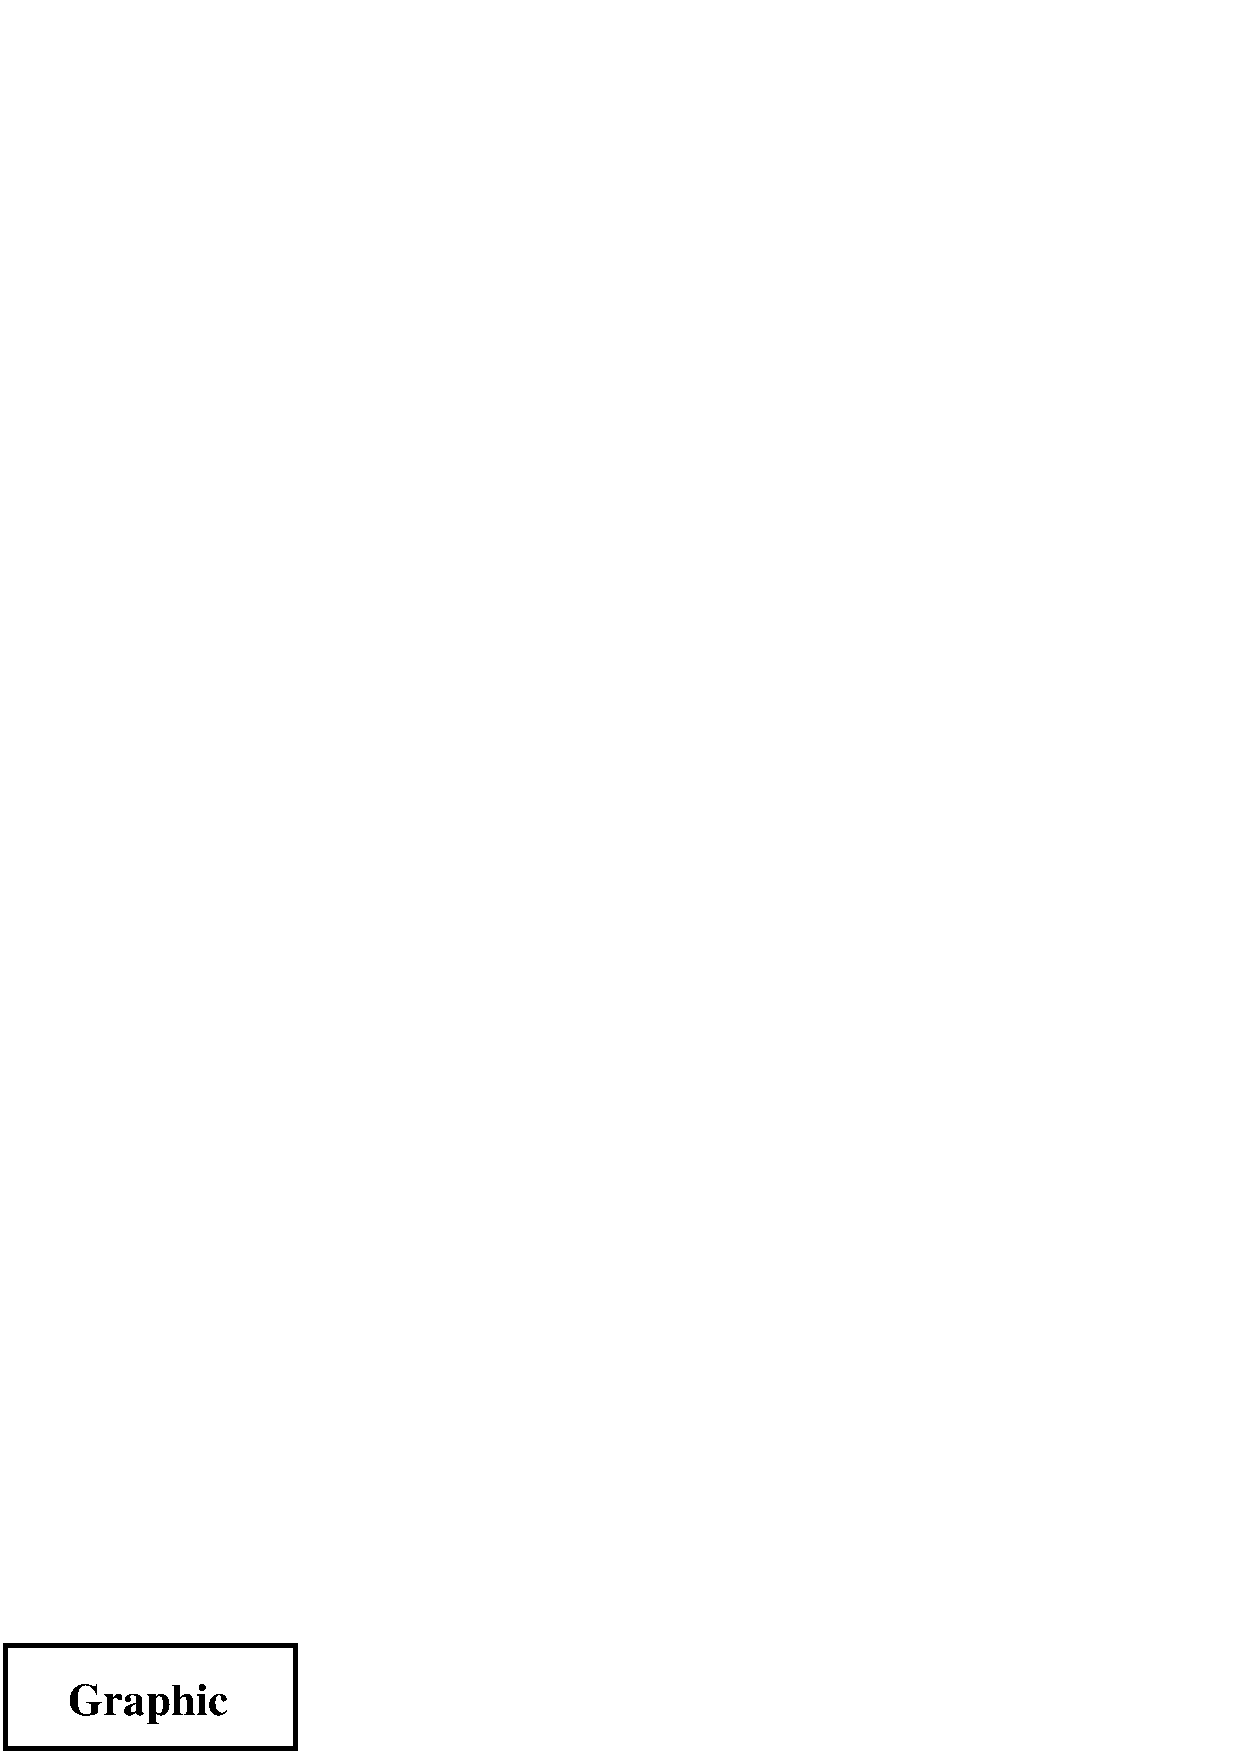
\includegraphics[width=0.80\linewidth]{graphic}
\end{lstlisting}
	\item 当与 \pkg{calc} 宏包配合使用时,
	如下命令可以使得插入图片的宽度比当前一行文本的宽度窄2英寸:
\begin{lstlisting}
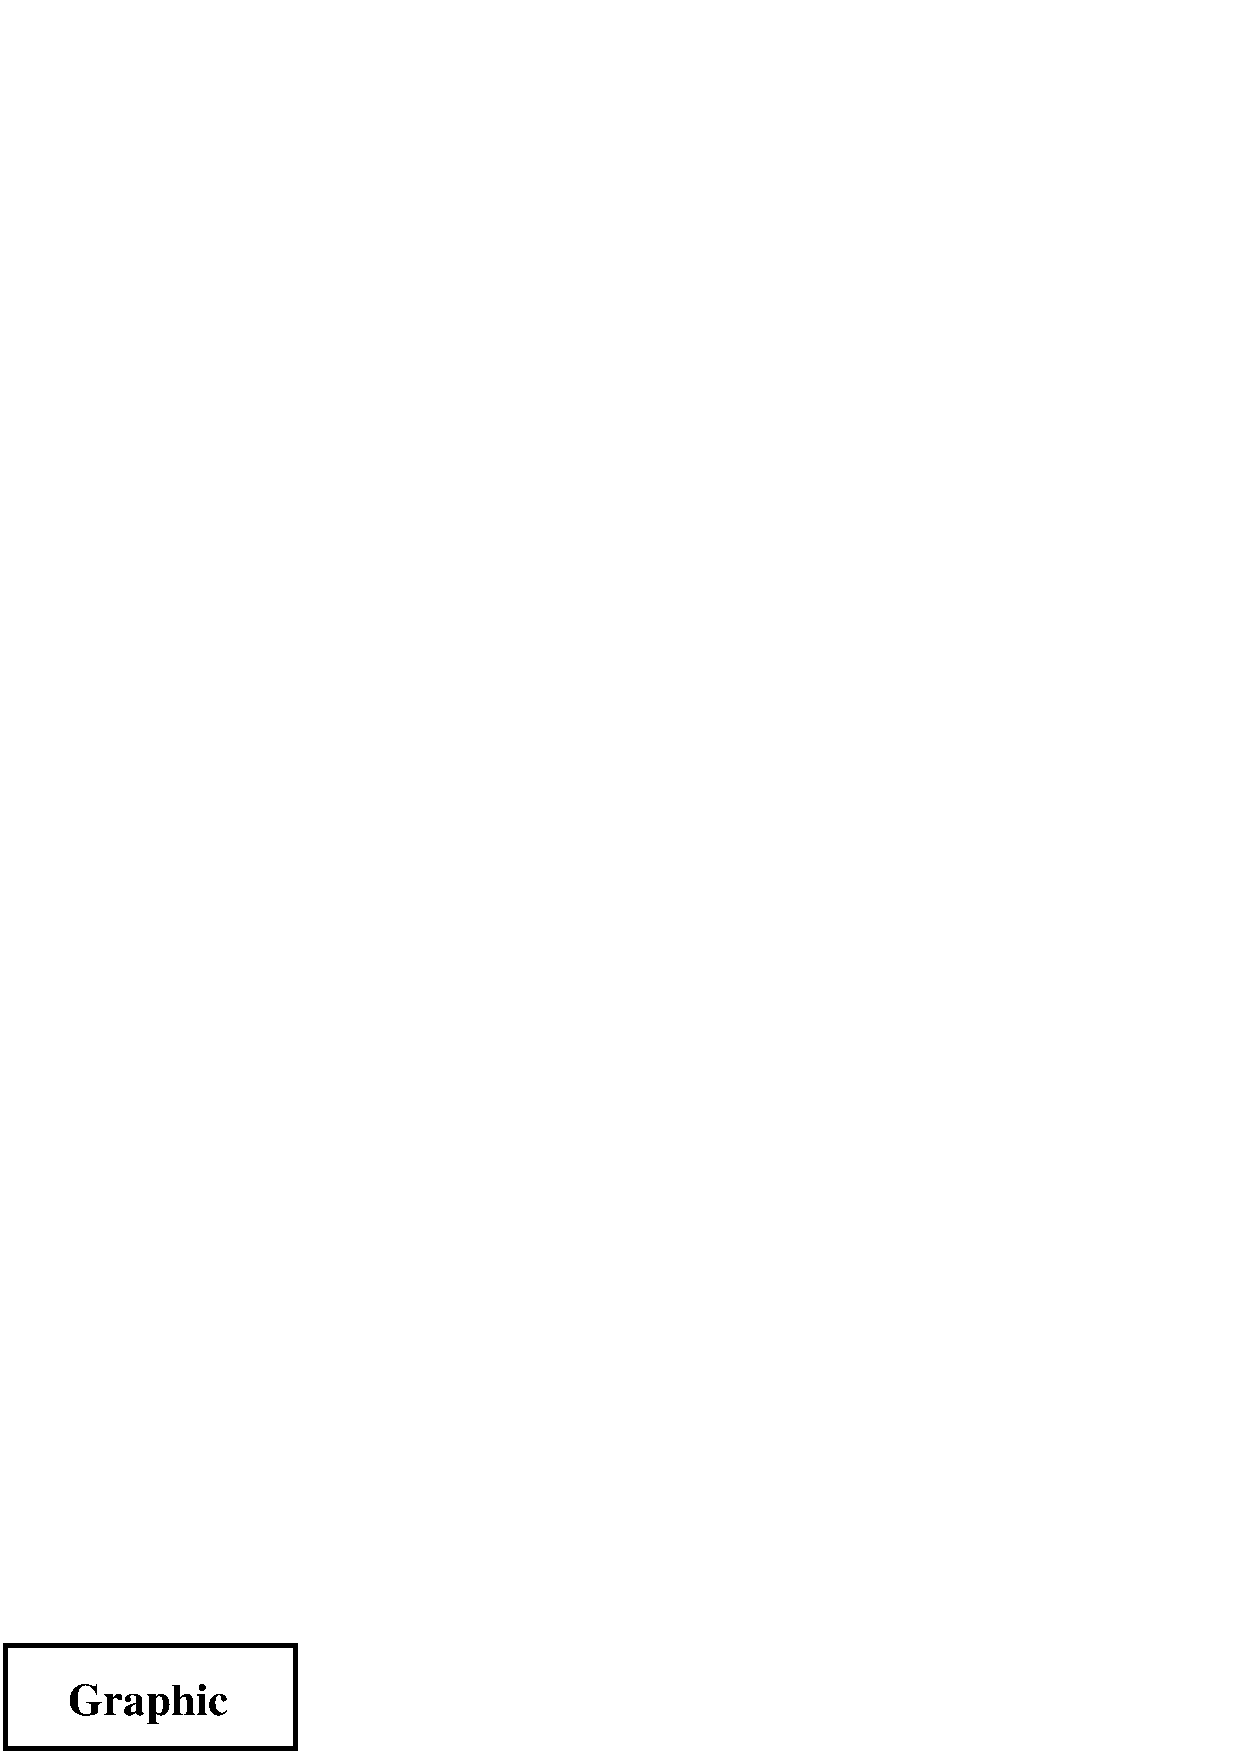
\includegraphics[width=\linewidth-2.0in]{graphic}
\end{lstlisting}
	
\end{itemize}

类似地,如下命令
\marginpar{指定高度}
\begin{lstlisting}
\includegraphics[height=2cm]{file}
\end{lstlisting}
导入指定的图片文件,且使得高度为2厘米。
此外,\cmd{includegraphics} 命令还有一个 \opt{totalheight} 选项来指定整体高度
(关于高度和整体高度的定义可参见第~\pageref{sec:terminology} 页的第~\ref{sec:terminology} 节)。

\cmd{includegraphics} 命令的 \opt{angle} 选项可以指定插入图像的角度:
\marginpar{指定角度}
\begin{lstlisting}
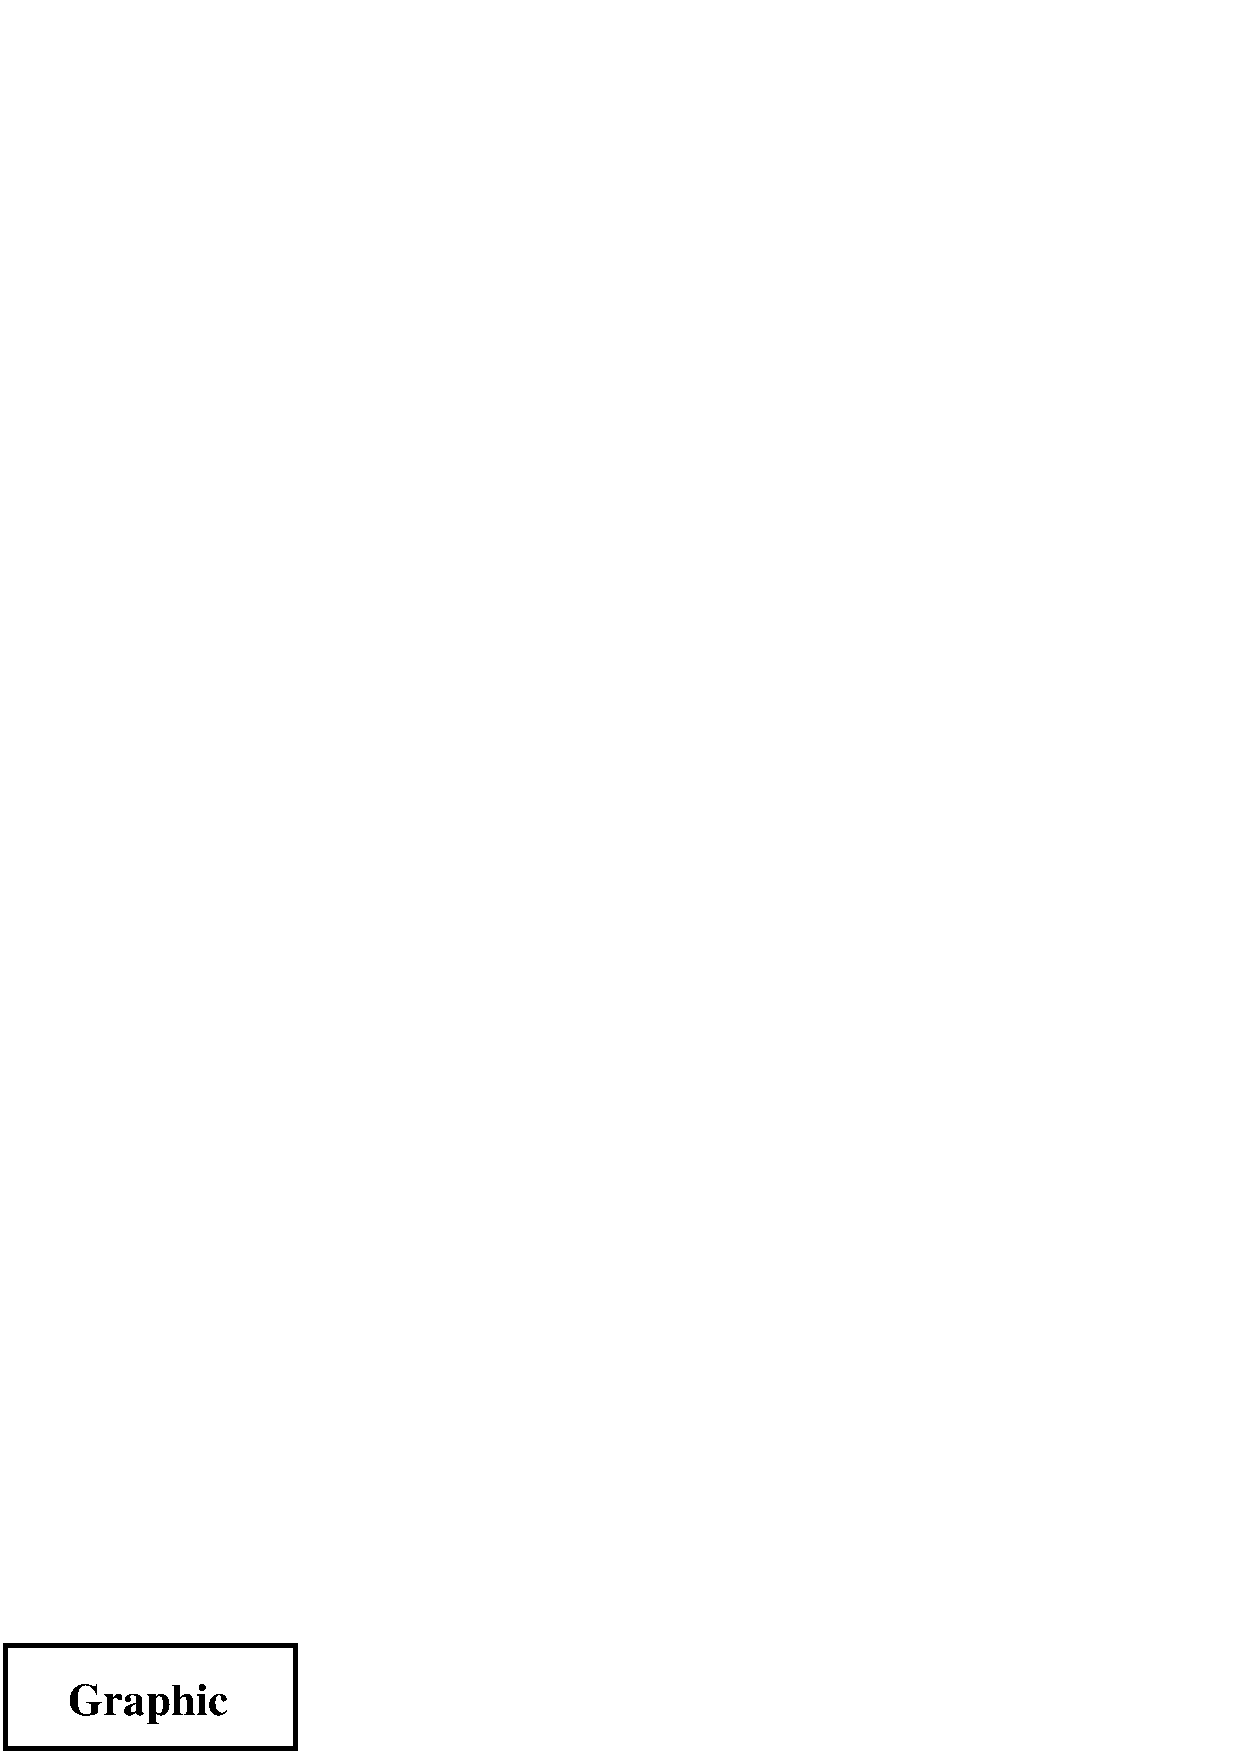
\includegraphics[angle=45]{graphic}
\end{lstlisting}
该命令会按照原始尺寸插入图片,并且按逆时针旋转45度。

\subsubsection{同时指定角度和高度/宽度}
由于 \cmd{includegraphics} 的选项是从左到右依次解释的,
所以其中指定角度和大小顺序会导致不同的效果。例如
\begin{lstlisting}
\begin{center}
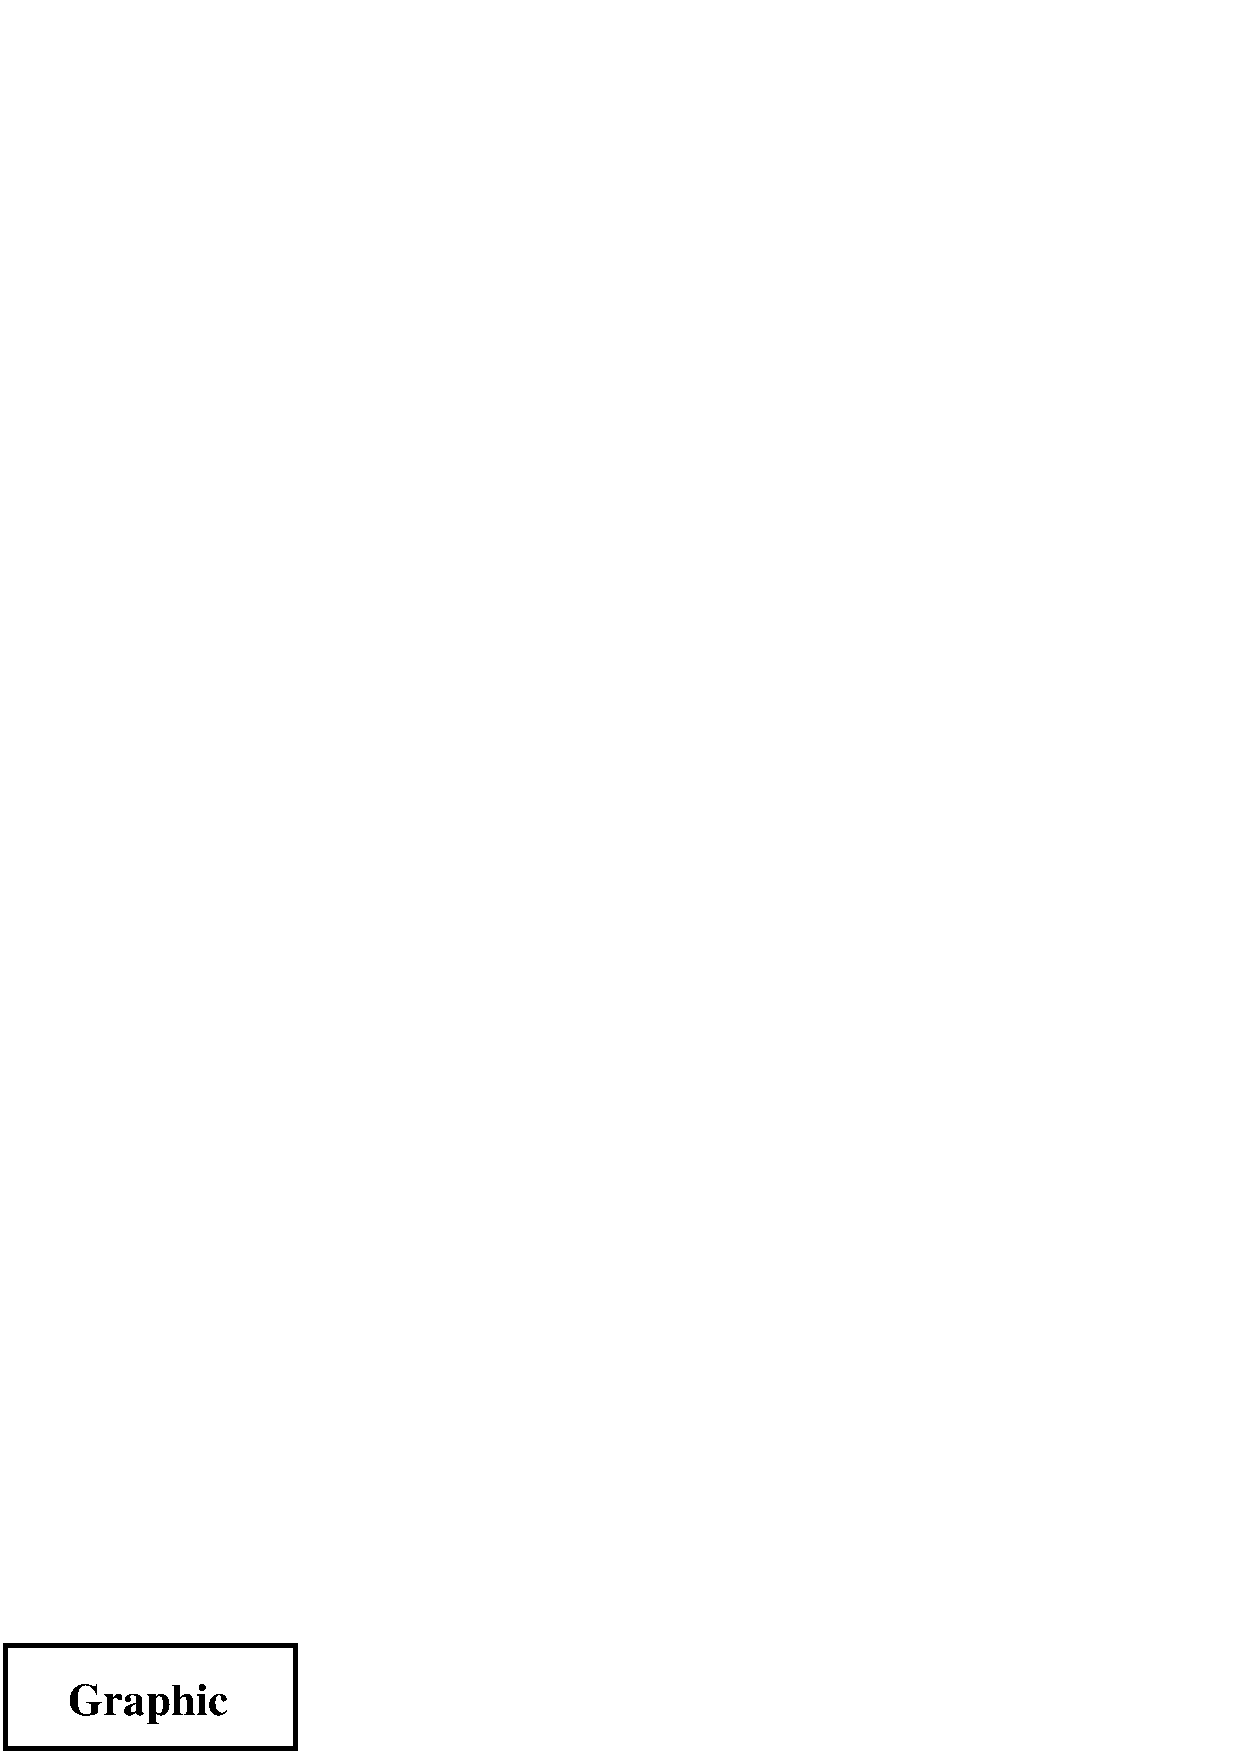
\includegraphics[angle=90,totalheight=1cm]{graphic}
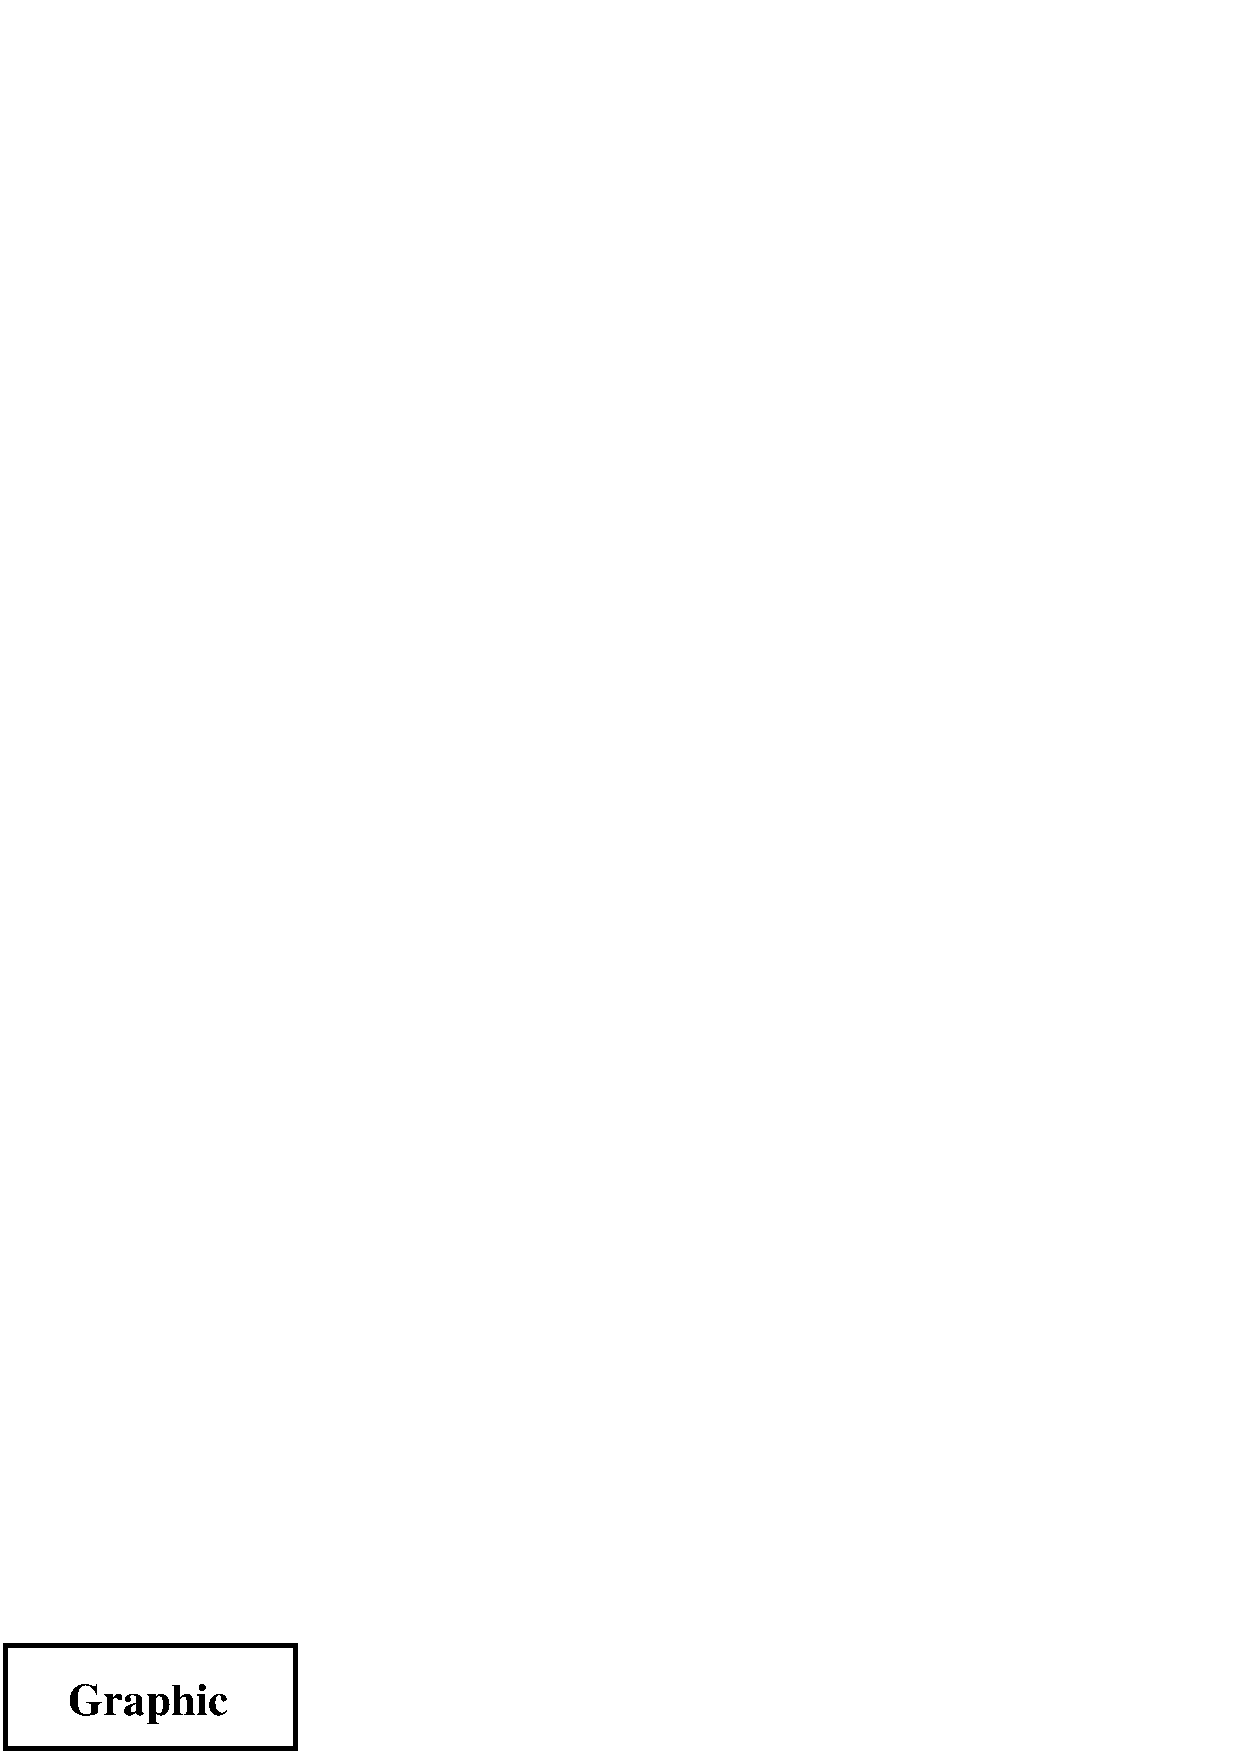
\includegraphics[totalheight=1cm,angle=90]{graphic}
\end{center}
\end{lstlisting}
会生成如下结果
\begin{center}
	\resizebox*{!}{1cm}{\rotatebox{90}{\usebox{\boxgraphic}}}
	\rotatebox{90}{\resizebox*{!}{1cm}{\usebox{\boxgraphic}}}
\end{center}
第一个盒子是先旋转了90度,然后缩放使得整体高度为1厘米。
第二个盒子先缩放使得整体高度为1厘米,然后再旋转90度。
另外要注意的是,以上图形中两幅图像之间有一个空格,
因为第一行 \cmd{includegraphics} 的末尾并没有以 \texttt{\%} 结束。

\begin{table}
\centering
\caption{\cmd{includegraphics} 选项}\label{tab:opt}
\begin{tabular}{>{\ttfamily}l p{0.7\textwidth}}
	\toprule
	height & 图形的高度,可用任何 \TeX{} 度量单位。 \\ \hline
	totalheight & 图形的整体高度,可用任何 \TeX{} 度量单位。 \\ \hline
	width & 图形的宽度,可为任何 \TeX{} 度量单位。 \\ \hline
	scale & 图形的缩放因子,设定 \opt{scale=2} 会使插入图形的大小为其自然大小的两倍。 \\ \hline
	angle & 设定旋转的角度,以度为单位,逆时针方向为正。 \\ \hline
	origin & \opt{origin} 指定图形绕那一点旋转,默认是围绕参考点旋转。
		\opt{origin} 点可以与第~\ref{ssec:rotatebox}节的 \cmd{rotatebox} 命令中的一样。
	比如 \opt{origin=c} 将使图形绕它的中心旋转。  \\ \hline
	bb & 设定 BoundingBox 的值。
	例如,\opt{bb=10 20 100 200} 会设定BoundingBox 的左下角在 $(10,20)$,右上角在 $(100,200)$。\par
	因为 \cmd{includegraphics} 会自动从 \file{eps} 文件中读入BoundingBox值,
	所以一般不用\opt{bb} 这个选项。
	但它在 \file{eps} 文件中的 BoundingBox 丢失或不准确时还是很有用的。 \\ 
	\bottomrule
\end{tabular}
\end{table}

\begin{table}
\centering
\caption{\cmd{includegraphics} 裁剪选项}\label{tab:cropopt}
\begin{tabular}{>{\ttfamily}l p{0.7\textwidth}}
	\toprule
	viewpoint & 指定图像可以被看到的部分。
	如同 BoundingBox 一样,这个区域由四个数字决定,分别是左下角和右上角的坐标。
	这里的坐标是以 BoundingBox 左下角为起点的相对坐标。
	
	例如,如果图像的 BoundingBox 的值是 \texttt{50	50 410 302},
	那么 \texttt{viewpoint=50 50 122 122} 显示的图像是一平方英寸大小的正方形区域,且以图像左下角为左下角。
	而 \texttt{viewpoint=338 230 410 302} 显示的图像也是一平方英寸大小的正方形区域,但以图形的右上角为右上角。
	
	必须使用\opt{clip} 选项(见表~\ref{tab:boolopt})来阻止显示视图以外的部分。 \\ \hline
	trim & 显示部分图像的另一种方法。
	所给出的四个数字分别代表了从左、下、右、上被截去的值。
	正数代表从此方向截去的大小,而负数则代表从此方向加上的大小。
	
	例如,\opt{trim=1 2 3 4} 代表图像的左边截去1 \texttt{bp},
	下边截去2 \texttt{bp},右边截去3 \texttt{bp},上边截去4 \texttt{bp}。
	
	必须使用\opt{clip} 选项(见表~\ref{tab:boolopt})来阻止显示被截去的部分。 \\ \bottomrule
\end{tabular}
\end{table}

\begin{table}
\centering
\caption{\cmd{includegraphics} 布尔型选项}\label{tab:boolopt}
\begin{tabular}{>{\ttfamily}l p{0.7\textwidth} }
	\toprule
	clip & 指定 \opt{clip=false} 会显示整个的图形,即使有些部分在视图之外。(默认值)
	
	指定 \opt{clip=true} 时将不显示图形在视图之外的部分。 \\ \hline
	draft & 使用\opt{draft} 或 \opt{draft=true} 选项将阻止图像的导入。
	此时在插图的位置只显示图像的BoundingBox和文件名,
	这会加快文档的显示和打印速度。
	使用 \opt{draft=false} 则会显示图像。
	
	如果使用 \opt{draft} 宏包选项 \cmdOM{usepackage}{draft}{graphicx},
	那么文档中的所有图像都以\opt{draft} 方式插入。  \\ \hline
	keepaspectratio & 在没有设定\opt{keepaspectratio} 选项时,
	如果同时给定图像的宽度和高度/整体高度,
	那么为了满足所设定的高和宽,图像的缩放可能会失真变形。
	
	在设定\opt{keepaspectratio} 选项后,给定图像的宽度和高度/整体高度时,
	图像会在保持原有的宽高比例下缩放,尽可能使得图像满足所设定的高和宽,
	但是图像的实际宽高不会超出设置的值。 \\ \bottomrule
\end{tabular}
\end{table}


\subsection{一些例子}

下面是一些使用 \cmd{includegraphics} 命令来插入图形的例子。\footnote{
	本小节来自于王磊在旧版本的中译本《\LaTeXe{} 插图指南》中额外补充的内容。——译注}
这里为方便起见,定义水平线 \cmd{HR} 为
\begin{lstlisting}
\newcommand{\HR}{\rule{1em}{0.4pt}}
\end{lstlisting}

\ifxetex\relax\else\ifpdf\relax\else %因为使用pdflatex不支持clip.所以省去。
在下面的几个例子中可以看到使用\opt{bb,clip,viewport} 和\opt{trim}的效果。

\hspace{-1cm}\begin{minipage}[c]{.5\textwidth}
	左\HR%
	\fbox{%
		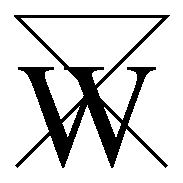
\includegraphics[bb=120 120 150 200]{w.eps}}%
	\HR 右
	\qquad
	左\HR%
	\fbox{%
		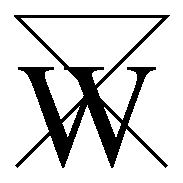
\includegraphics[bb=120 120 150 200,clip]{w.eps}}%
	\HR 右
\end{minipage}%
\begin{minipage}[c]{.5\textwidth}
	\begin{Verbatim}[frame=lines,label=\colorbox{green}{\small 例一},labelposition=topline,]
	左\HR\fbox{%
	\includegraphics
	[bb=120 120 150 200]%
	{w.eps}}%
	\HR 右
	\qquad
	左\HR\fbox{%
	\includegraphics
	[bb=120 120 150 200,clip]%
	{w.eps}}%
	\HR 右
	\end{Verbatim}
\end{minipage}

\hspace{-1.5cm}\begin{minipage}[c]{.65\textwidth}
	左\HR\fbox{%
		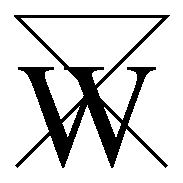
\includegraphics[viewport=20 20 50 100,clip]{w}}%
	\HR 右
	\qquad
	左\HR\fbox{%
		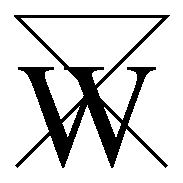
\includegraphics[trim=5 5 10 10,clip]{w}}%
	\HR 右
\end{minipage}%
\hspace{-1cm}\begin{minipage}[c]{.5\textwidth}
	\begin{Verbatim}[frame=lines,label=\colorbox{green}{\small 例二},labelposition=topline]
	左\HR\fbox{%
	\includegraphics
	[viewport=20 20 50 100,clip]%
	{w.eps}}%
	\HR 右
	\qquad
	左\HR\fbox{%
	\includegraphics
	[trim=5 5 10 10,clip]%
	{w.eps}}
	\HR 右
	\end{Verbatim}
	\par\vspace{0pt}
\end{minipage}
\fi\fi

以下几个例子中使用了 \opt{scale}、\opt{width}、\opt{height}、\opt{angle} 以及 \opt{keepaspectratio} 等选项及其不同的顺序,从而得到的不同效果。

\begin{minipage}[t]{.45\textwidth}
	\vspace{0pt}
	左\HR\fbox{%
		\scalebox{0.5}{\usebox{\boxw}}}\HR 右
\end{minipage}%
\hspace{-.5cm}
\begin{minipage}[t]{.5\textwidth}
	\vspace{0pt}
\begin{Verbatim}[frame=lines,label=\colorbox{green}{\small 例一},labelposition=topline,formatcom=\color{VerbatimColor}]
左\HR\fbox{%
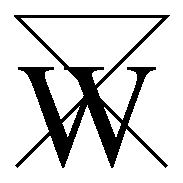
\includegraphics
[scale=.5]{w.eps}%
\HR 右
\end{Verbatim}
\end{minipage}

\begin{minipage}[c]{.45\textwidth}
	左\HR\fbox{%
		\resizebox{10mm}{!}{\usebox{\boxw}}}\HR 右
\end{minipage}%
\hspace{-.5cm}
\begin{minipage}[c]{.5\textwidth}
\begin{Verbatim}[frame=lines,label=\colorbox{green}{\small 例二},labelposition=topline,formatcom=\color{VerbatimColor}]
左\HR\fbox{%
\includegraphics%
[width=10mm]{w.eps}%
\HR 右
\end{Verbatim}
\end{minipage}

\begin{minipage}[c]{.45\textwidth}
	左\HR\fbox{%
		\resizebox{20mm}{30mm}{\usebox{\boxw}}}\HR 右
\end{minipage}%
\hspace{-.5cm}
\begin{minipage}[c]{.5\textwidth}
\begin{Verbatim}[frame=lines,label=\colorbox{green}{\small 例三},labelposition=topline,formatcom=\color{VerbatimColor}]
左\HR\fbox{%
\includegraphics
[height=20mm,width=30mm]%
{w.eps}}\HR 右
\end{Verbatim}
\end{minipage}

\begin{minipage}[c]{.45\textwidth}
	左\HR\fbox{%
		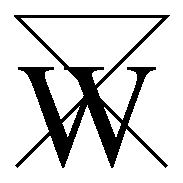
\includegraphics[height=20mm,width=30mm,%
		keepaspectratio]{w}}\HR 右
\end{minipage}%
\hspace{-.5cm}
\begin{minipage}[c]{.5\textwidth}
\begin{Verbatim}[frame=lines,label=\colorbox{green}{\small 例四},labelposition=topline,formatcom=\color{VerbatimColor}]
左\HR\fbox{%
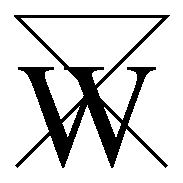
\includegraphics
[height=20mm,width=30mm,%
keepaspectratio]{w.eps}}%
\HR 右
\end{Verbatim}
\end{minipage}

\begin{minipage}[c]{.45\textwidth}
	左\HR\fbox{%
		\rotatebox{-45}{\usebox{\boxw}}}\HR 右
\end{minipage}%
\hspace{-.5cm}
\begin{minipage}[c]{.5\textwidth}
\begin{Verbatim}[frame=lines,label=\colorbox{green}{\small 例五},labelposition=topline,formatcom=\color{VerbatimColor}]
左\HR\fbox{%
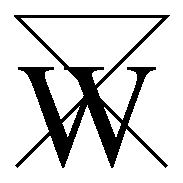
\includegraphics
[angle=-45]{w.eps}}%
\HR 右
\end{Verbatim}
\end{minipage}

\begin{minipage}[c]{.45\textwidth}
	左\HR\fbox{%
		\resizebox{30mm}{!}{\rotatebox{-45}{\usebox{\boxw}}}}\HR 右
\end{minipage}%
\hspace{-.5cm}
\begin{minipage}[c]{.5\textwidth}
\begin{Verbatim}[frame=lines,label=\colorbox{green}{\small 例六},labelposition=topline,formatcom=\color{VerbatimColor}]
左\HR\fbox{%
\includegraphics
[angle=-45,width=30mm]%
{w.eps}}\HR 右
\end{Verbatim}
\end{minipage}

\hspace{-1cm}
\begin{minipage}[c]{.45\textwidth}
	左\HR\fbox{%
		\rotatebox{-45}{\resizebox{30mm}{!}{\usebox{\boxw}}}}\HR 右
\end{minipage}%
\begin{minipage}[c]{.5\textwidth}
\begin{Verbatim}[frame=lines,label=\colorbox{green}{\small 例七},labelposition=topline,formatcom=\color{VerbatimColor}]
左\HR\fbox{%
\includegraphics
[width=30mm,angle=-45]%
{w.eps}}\HR 右
\end{Verbatim}
\end{minipage}

\begin{minipage}[c]{.45\textwidth}
	左\HR\fbox{%
		\resizebox*{!}{15mm}{\rotatebox{-60}{\usebox{\boxw}}}}%
	\HR 右
\end{minipage}%
\hspace{-.5cm}
\begin{minipage}[c]{.5\textwidth}
\begin{Verbatim}[frame=lines,label=\colorbox{green}{\small 例八},labelposition=topline,formatcom=\color{VerbatimColor}]
左\HR\fbox{%
\includegraphics
[angle=-60,totalheight=15mm]%
{w.eps}}%
\HR 右
\end{Verbatim}
\end{minipage}

\begin{minipage}[c]{.45\textwidth}
	左\HR\fbox{%
		\resizebox*{30mm}{20mm}{\rotatebox{-60}{\usebox{\boxw}}}}%
	\HR 右
\end{minipage}%
\hspace{-.5cm}
\begin{minipage}[c]{.5\textwidth}
\begin{Verbatim}[frame=lines,label=\colorbox{green}{\small 例九},labelposition=topline,formatcom=\color{VerbatimColor}]
左\HR\fbox{%
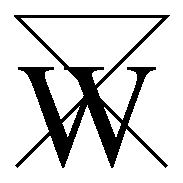
\includegraphics
[angle=-60,totalheight=20mm,%
width=30mm]{w.eps}}%
\HR 右
\end{Verbatim}
\end{minipage}

\begin{minipage}[c]{.45\textwidth}
	左\HR\fbox{%
		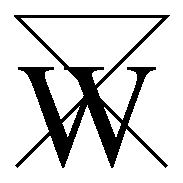
\includegraphics[angle=-60,totalheight=20mm,width=30mm,keepaspectratio]{w}}%
	\HR 右
\end{minipage}%
\hspace{-.5cm}
\begin{minipage}[c]{.5\textwidth}
\begin{Verbatim}[frame=lines,label=\colorbox{green}{\small 例十},labelposition=topline,formatcom=\color{VerbatimColor}]
左\HR\fbox{%
\includegraphics
[angle=-60,totalheight=20mm,%
width=30mm,keepaspectratio]%
{w.eps}}%
\HR 右
\end{Verbatim}
\end{minipage}

\section{旋转和缩放对象}\label{sec:scalerotate}
除了 \cmd{includegraphics}命令外,
\pkg{graphicx} 宏包还提供了另外四个命令用来旋转和缩放任意的 \LaTeX{} 对象,例如文本、图像等。
\begin{lstlisting}
\scalebox{水平缩放因子}[垂直缩放因子]{对象}
\resizebox{宽度}{高度}{对象}
\resizebox*{宽度}{整体高度}{对象}
\rotatebox[选项]{角度}{对象}
\end{lstlisting}

因为 \pkg{graphicx} 包的 \cmd{includegraphics} 已经带有 \opt{angle}、\opt{width} 等支持旋转和缩放的选项,
所以本节介绍的这几个命令很少在插图时使用。例如:
\begin{lstlisting}
\includegraphics[scale=2]{file.eps}
\includegraphics[width=4in]{file.eps}
\includegraphics[angle=45]{file.eps}
\end{lstlisting}
上述命令和下面的命令等到的结果是相同的。
\begin{lstlisting}
\scalebox{2}{\includegraphics{file.eps}}
\resizebox{4in}{!}{\includegraphics{file.eps}}
\rotatebox{45}{\includegraphics{file.eps}}
\end{lstlisting}

尽管结果相同,但最好还是用前一种方法,
因为它的速度更快,而且生成 PostScript 和 \file{pdf} 的效率更高。

\subsection{scalebox 命令}\label{ssec:scalebox}
语法:
\begin{lstlisting}
\scalebox{水平缩放因子}[垂直缩放因子]{对象}
\end{lstlisting}

\cmdi{scalebox} 命令对其作用的对象进行缩放,
使得缩放后对象的宽度为原始宽度与“\texttt{水平缩放因子}”之积,高度为原始高度与“\texttt{垂直缩放因子}”之积。
如果“\texttt{垂直缩放因子}”没有给出,那么默认取为“\texttt{水平缩放因子}”,
以保持原始的宽高比进行缩放。
如果缩放因子为负值,则翻转该对象。下面是几个例子

%\hspace{-1.5cm}
\begin{center}
\begin{minipage}[b]{.5\textwidth}
	\begin{center}
		\color{blue}{\CJKfamily{zhkai}
			\scalebox{2}{这是放大的文字} \\
			这是正常的文字 \\
			\scalebox{.5}{这是缩小的文字}}
	\end{center}
	\par\vspace{0pt}
\end{minipage}%
\begin{minipage}[b]{.5\textwidth}
\begin{lstlisting}
\scalebox{2}{这是放大的文字} \\
这是正常的文字  \\
\scalebox{.5}{这是缩小的文字}
\end{lstlisting}
\par\vspace{0pt}
\end{minipage}
\end{center}

\begin{center}
%\hspace{-1.5cm}
\begin{minipage}[b]{.5\textwidth}
	\color{blue}{\CJKfamily{zhkai}
		\framebox{\scalebox{2}{%
				\parbox{.5in}{放大 \\ 和 \\ 缩小}}}
		\framebox{\scalebox{2}[1.5]{%
				\parbox{.5in}{放大 \\ 和 \\ 缩小}}}}
	\par\vspace{0pt}
\end{minipage}%
\begin{minipage}[b]{.5\textwidth}
\begin{lstlisting}
\framebox{\scalebox{2}{%
\parbox{.5in}{放大 \\ 和 \\ 缩小}}}
\framebox{\scalebox{2}[1.5]{%
\parbox{.5in}{放大 \\ 和 \\ 缩小}}}
\end{lstlisting}
\par\vspace{0pt}
\end{minipage}	
\end{center}

\begin{center}
%\hspace{-1.5cm}
\begin{minipage}[b]{.5\textwidth}
	\begin{center}
		\color{blue}{\texttt{%
				China? \scalebox{-1}[1]{China?} \\
				China? \scalebox{1}[-1]{China?} \\
				China? \scalebox{-1}[-1]{China?} \\
				China? \scalebox{-1}{China?}}}
	\end{center}
	\par\vspace{0pt}
\end{minipage}%
\begin{minipage}[b]{.5\textwidth}
\begin{lstlisting}
China? \scalebox{-1}[1]{China?} \\
China? \scalebox{1}[-1]{China?} \\
China? \scalebox{-1}[-1]{China?} \\
China? \scalebox{-1}{China?}}
\end{lstlisting}
\par\vspace{0pt}
\end{minipage}
\end{center}


\subsection{resizebox 命令}\label{ssec:resizebox}
语法:
\begin{lstlisting}
\resizebox{宽度}{高度}{对象}
\resizebox*{宽度}{整体高度}{对象}
\end{lstlisting}

\cmdi{resizebox} 命令将对象的大小改变为给定值。
如果“\texttt{宽度}”或“\texttt{高度}”中的任一项用 \texttt{!} 给出,
那么缩放时会保持原有的宽高比。
例如:
\begin{lstlisting}
\resizebox{2in}{!}{argument}
\end{lstlisting}
将对象的宽度改变为2英寸,同时保持宽高比。

标准的 \LaTeXe{} 长度命令 \cmd{height}、\cmd{width}、\cmd{totalheight}、\cmd{depth} 可用来表示对象的原始尺寸。
因此,
\begin{lstlisting}
\resizebox{2in}{\height}{argument}
\end{lstlisting}
使得对象的宽度改变为 2 英寸但保持原有高度不变。 

此外,命令 \cmdi{reseizebox*} 与 \cmd{resizebox} 几乎是相同的,
不同之处仅在于第二个参数表示对象的整体高度。
(关于高度和整体高度的定义见第~\ref{sec:terminology} 节,
关于 \opt{height} 和 \opt{totalheight} 选项的比较见第~\ref{ssec:diffheight} 节。)

下面是几个例子:

\begin{center}
%\hspace{-1.5cm}
\begin{minipage}[b]{.4\textwidth}
	\begin{center}
		\color{blue}{\CJKfamily{zhkai}
			\framebox{\resizebox{5mm}{!}{%
					\parbox{14mm}{选项 \\ 角度 \\ 对象}}}
			\framebox{\resizebox{!}{10mm}{%
					\parbox{14mm}{选项 \\ 角度 \\ 对象}}}}
		\par\vspace{0pt}
	\end{center}
\end{minipage}%
\hspace{-1cm}
\begin{minipage}[b]{.6\textwidth}
\begin{lstlisting}
\framebox{\resizebox{5mm}{!}{%
\parbox{14mm}{选项 \\ 角度 \\ 对象}}}
\framebox{\resizebox{!}{10mm}{%
\parbox{14mm}{选项 \\ 角度 \\ 对象}}}
\end{lstlisting}
\par\vspace{0pt}
\end{minipage}
\end{center}

\begin{center}
%\hspace{-2cm}
\begin{minipage}[b]{.4\textwidth}
	\begin{center}
		\color{blue}{\CJKfamily{zhkai}
			\resizebox*{2cm}{3cm}{\LaTeX{}~图形} \\
			\resizebox*{2cm}{1cm}{\LaTeX{}~图形}}
		\par\vspace{0pt}
	\end{center}
\end{minipage}%
\begin{minipage}[b]{.6\textwidth}
\begin{lstlisting}
\resizebox*{2cm}{3cm}{\LaTeX{}~图形} \\
\resizebox*{2cm}{1cm}{\LaTeX{}~图形}
\end{lstlisting}
\par\vspace{0pt}
\end{minipage}
\end{center}


\subsection{rotatebox 命令}\label{ssec:rotatebox}
语法:
\begin{lstlisting}
\rotatebox[选项]{角度}{对象}
\end{lstlisting}
\cmdi{rotatebox} 将对象旋转一给定度数的角度,逆时针方向为正。
默认选项下对象绕它的参考点旋转。
\cmd{rotatebox} 命令中“\texttt{选项}”允许对象绕给定的点来旋转。
\begin{enumerate}
	\item 给定\opt{[x=xdim,y=ydim]},则对象旋转所绕的点相对于参考点的
	坐标为 $(\mathtt{xdim}, \mathtt{ydim})$。
	\item \opt{origin} 选项可以指定12个特殊点其中之一(见图~\ref{fig:rotatepoint})。
\end{enumerate}

\opt{origin} 点的水平位置由 \opt{lcr}(分别代表左、中、右)三个字母其中之一确定,
垂直位置则由 \opt{t,c,B,b}(分别代表顶部、中部、基线、底部)四个字母中的一个来确定。
例如:
\begin{description}
	\item [\opt{[rb]}] 右下角。
	\item [\opt{[lt]}] 左上角。
	\item [\opt{[cB]}] 图形基线的中点。
\end{description}

\paragraph{几点说明:}
\begin{itemize}
	\item 标记字母的顺序并不重要,\opt{[br]} 等同于 \opt{[rb]}。
	\item \opt{c} 代表水平位置的中点还是垂直位置的中点由和它一起的标记字母来决定。
	\item 如果只给出一个标记字母,那么另一个将被假设为 \opt{c}。
	即,\opt{[c]} 等于\opt{[cc]},\opt{[l]}等于\opt{[lc]},\opt{[t]}等于\opt{[ct]},等等。
\end{itemize}

\begin{figure}
	\centering
	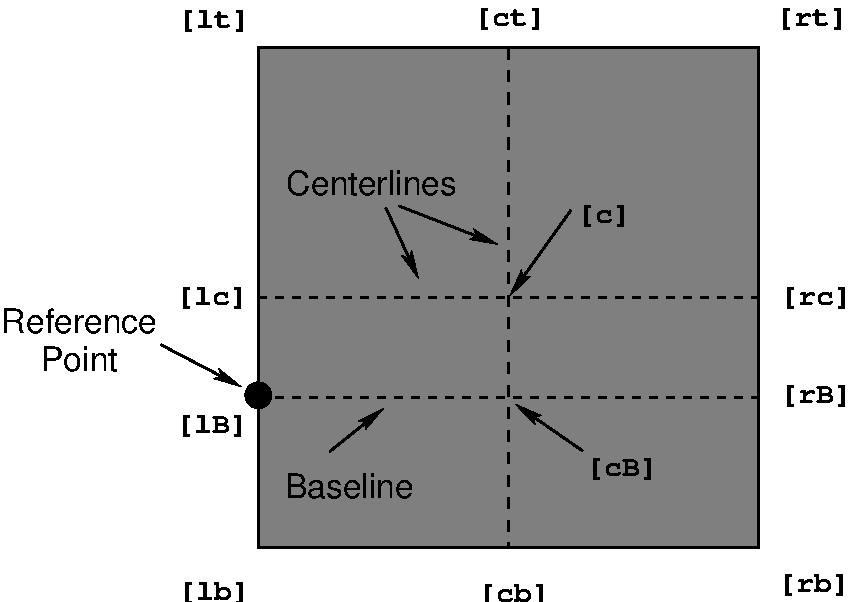
\includegraphics[width=.6\textwidth]{orig-point}
	\caption{可用的 \opt{origin} 点}\label{fig:rotatepoint}
\end{figure}

下面是一个例子:

\begin{center}
%\hspace{-1.5cm}
\begin{minipage}[b]{.4\textwidth}
	\begin{center}
		\setlength{\fboxsep}{0mm}
		\newcommand{\MyRot}[1]{%
			\fbox{\rotatebox{#1}{旋转~$#1^\circ$}}}
		\color{blue}{\CJKfamily{zhkai}
			\MyRot{0} \MyRot{45} \MyRot{90}
			\MyRot{135} \MyRot{180} \MyRot{225}}
	\end{center}
	\par\vspace{0pt}
\end{minipage}%
\begin{minipage}[b]{.6\textwidth}
\begin{lstlisting}
\setlength{\fboxsep}{0mm}
\newcommand{\MyRot}[1]{%
\fbox{\rotatebox{#1}{旋转~$#1^\circ$}}}
\MyRot{0} \MyRot{45} \MyRot{90}
\MyRot{135} \MyRot{180} \MyRot{225}
\end{lstlisting}
\par\vspace{0pt}
\end{minipage}
\end{center}


\section{高级插图命令}\label{sec:adgraphcmd}
本节描述了一些 \LaTeXe{} 图形宏包套件的高级命令,
用于下述情形。
\begin{enumerate}
	\item 当使用没有扩展名的文件名时。如:
\begin{lstlisting}
\includegraphics{file}
\end{lstlisting}

	\item 当使用压缩的\file{eps} 图形文件时。见第~\ref{ssec:compresseps} 节。
	\item 当使用非\file{eps} 格式的图形文件时。见第~\ref{ssec:noneps} 节。
\end{enumerate}
在这些情况下,\LaTeX{} 为了处理由命令 \cmd{includegraphics} 所导入的图像文件,
就需要用 \cmdi{DeclareGraphicsRule} 和 \cmdi{DeclareGraphicsExtensions} 命令来控制。
\begin{itemize}
	\item \cmd{DeclareGraphicsExtensions} 命令指定了在没有提供图形文件扩展名的情况下,
	\LaTeX{} 将自动为其加上的扩展名列表(如 \file{.eps}、\file{.ps}、\file{.eps.gz} 等)。
	\item \cmd{DeclareGraphicsRule} 命令指定了对图形文件执行的命令。
	执行这一命令要求操作系统支持管道功能,比如 Unix 等操作系统,而DOS则不行。
	
	若将此命令指定为一解压缩命令,那么就可以使用压缩的 \file{eps} 图形文件。
	若将此命令指定为一图形格式转换命令,那么就可以使用非\file{eps} 格式的图形文件。
\end{itemize}

\subsection{DeclareGraphicsExtensions 命令}\label{ssec:deextension}
\cmd{DeclareGraphicsExtensions} 命令告诉 \LaTeX{},
若 \cmd{includegraphics} 命令所引入的文件没有提供扩展名,
将试图为其自动加上什么样的扩展名。

为方便起见,在选择图形驱动\footnote{
	指定一个图形驱动选项如 \cmdOM{usepackage}{dvips}{graphics} 将会覆盖掉在 \texttt{graphics.cfg} 中设定的缺省驱动选项——旧译本注。}
时,就已经有一个相应的预设扩展名集。
举例来说,如果选择 \prgname{dvips} 作为图形驱动,
那么默认会使用下列图形文件扩展名(在 \file{dvips.def} 中定义):
\begin{lstlisting}
\DeclareGraphicsExtensions{.eps,.ps,.eps.gz,.ps.gz,.eps.Z}
\end{lstlisting}

如果 \pkg{graphicx} 宏包使用 \prgname{pdftex} 驱动,
那么默认会使用下列图形文件扩展名(在 \file{pdftex.def} 中定义)\footnote{
    实际上在较新版本(2016年)中,\file{dvips.def} 中定义扩展名的方式为
	\begin{flushleft}
		\cmd{def}\cmdM{Gin@extions}{.eps,.ps,.eps.gz,.ps.gz,.eps.Z,.mps}
	\end{flushleft}
	\file{pdftex.def} 中定义扩展名的方式为
	\begin{flushleft}
		\cmd{def}\cmdM{Gin@extions}{.png,.pdf,.jpg,.mps,.jpeg,.PNG,.PDF,.JPG,.JPEG}
	\end{flushleft}
	——译注}:
\begin{lstlisting}
\DeclareGraphicsExtensions{.png,.pdf,.jpg,.mps}
\end{lstlisting}

在 \opt{dvips} 图像扩展名列表中,
\cmdM{includegraphics}{file} 首先寻找 \file{file.eps},
其次是 \file{file.ps},再其次是 \texttt{file.eps.gz},直到找到一个文件。
相应地,可以用
\begin{lstlisting}
\includegrapincs{file}
\end{lstlisting}
取代
\begin{lstlisting}
\includegrapincs{file.eps}
\end{lstlisting}
这样做的好处是如果以后决定压缩 \file{file.eps},也无须更改 \LaTeX{} 文件。
无后缀名的方式使得可以同时使用 \LaTeX{} 和 \pdfLaTeX{} 编译文档,
见第~\pageref{ssec:latexandpdflatex} 页的 \ref{ssec:latexandpdflatex} 节。
然而,这种无后缀名的方式可能会加剧内存池空间问题,详见下面的~\ref{sssec:poolspaceproblem} 小节。

\subsubsection{无扩展名的文件}
需要注意的是,
\begin{lstlisting}
\includegrapincs{file}
\end{lstlisting}
不会试图寻找 \file{file},
除非空扩展名列表中包含空的扩展名 \verb+{}+。
例如:
\begin{lstlisting}
\DeclareGraphicsExtensions{.eps,.eps.gz,{}}
\end{lstlisting}
将试图在没找到 \file{file.eps} 和 \file{file.eps.gz} 的情况下寻找 \file{file}。

由于默认的扩展名列表中不包含空扩展名,
如果想要使用无扩展名文件的话,
必须使用 \cmd{DeclareGraphicsExtensions} 命令定义一个包含空扩展名的列表。

\subsubsection{池空间问题}\label{sssec:poolspaceproblem}

不给出扩展名而靠 \LaTeX{} 从 \cmd{DeclareGraphicsExtensions} 的扩展名列表中选择正确的扩展名可能
加剧池空间问题(见第~\ref{ssec:poolspace} 节)。
如果有池空间问题的话,应当使用 \cmd{DeclareGraphicsExtensions} 指定的扩展名数目尽可能小。如:
\begin{lstlisting}
\DeclareGraphicsExtensions{.eps,.eps.gz}
\end{lstlisting}


\subsection{DeclareGraphicsRule 命令}\label{ssec:derule}
\cmdi{DeclareGraphicsRule} 命令指定 \cmd{includegraphics} 如何按照扩展名
来对操作图像文件。语法为
\begin{lstlisting}
\DeclareGraphicsRule{ext}{type}{sizefile}{command}
\end{lstlisting}
例如,如下命令
\begin{lstlisting}
\DeclareGraphicsRule{.eps.gz}{eps}{.eps.bb}{`gunzip -c #1}
\end{lstlisting}
指定任何以 \file{.eps.gz} 为扩展名的文件为压缩的\file{eps} 文件,
该文件的 BoundingBox 信息存放在扩展名为 \file{.eps.bb} 的文件中,
并用命令 \texttt{gunzip -c} 来解压缩
(因为 \LaTeX{} 不能从压缩文件中读取 BoundingBox 信息,
所以 BoundingBox 行必须存放到非压缩文件中)。

可以允许有多个 \cmd{DeclareGraphicsRule} 命令。

\cmd{DeclareGraphicsRule} 命令允许使用 \texttt{*} 代表任何未知扩展名,
例如:
\begin{lstlisting}
\DeclareGraphicsRule{*}{eps}{*}{}
\end{lstlisting}
会导致所有未知扩展名的文件都被认为是 \file{eps} 文件,
比方说 \file{file.EPS} 就被当做\file{eps} 文件。

\begin{table}
	\centering
	\caption{\cmd{DeclareGraphicsRule} 的选项}\label{tab:DeclaregruleArgs}
	\begin{tabular}{>{\ttfamily}l  p{0.7\textwidth}}
		\toprule
		ext & 文件的扩展名。 \\ \hline
		type & 扩展名所对应的图像类型。 \\ \hline
		sizefile & 包含图像 BoundingBox 信息的文件的扩展名。
		如果这一选项为空,
		那么必须要在 \cmd{includegraphics} 命令中给定 \opt{bb} 选项的值。 \\ \hline
		command & 作用于图像文件的命令,此项常为空。
		命令前必须有一个前单引号(键盘上数字键 \texttt{1} 左侧的键——译注),
		注意不是常用的后单引号。
		目前为止,只有 \prgname{dvips} 能够执行这样的命令。
		参见第~\ref{ssec:noneps} 节关于如何用这样的命令来处理非 \file{eps} 格式图像和压缩的 \file{eps} 图像的例子。\\
		\bottomrule
	\end{tabular}
\end{table}

文件的扩展名定义为文件名里第一个句点以后的部分,
\marginpar{文件名中的句点}
这样做是为了可以将 \file{.eps.gz} 结尾的文件识别成压缩的\file{eps} 文件。
为了避免混淆,文件的基本名中不要使用句点。
例如,指定文件 \file{file.name.eps.gz} 会让 \cmd{includegraphics} 寻找扩展名为 \file{.name.eps.gz} 所对应的图像规则。
由于这样的规则很有可能不存在,结果导致使用未知扩展名所对应的规则。
例外的情形是该文件的格式正好是缺省格式,
如果未知扩展名的文件都被认为是 \file{eps} 文件,
那么 \file{file.name.eps} 就恰巧能被正确地识别。

为方便起见,根据不同的图形驱动选项,
\marginpar{预定义命令}
已经预定义了不同的缺省图像规则。
例如使用 \opt{dvips} 图形驱动选项时,文件 \file{dvips.def} 定义了如下缺省图形规则\footnote{
	实际上 \file{dvips.def} 的代码并没有使用 \cmd{DeclareGraphicsRule},
	不过效果是一样的。}:
\begin{lstlisting}
\DeclareGraphicsRule{.eps}{eps}{.eps}{}
\DeclareGraphicsRule{.ps}{eps}{.ps}{}
\DeclareGraphicsRule{.pz}{eps}{.bb}{`gunzip -c #1}
\DeclareGraphicsRule{.eps.Z}{eps}{.eps.bb}{`gunzip -c #1}
\DeclareGraphicsRule{.ps.Z}{eps}{.ps.bb}{`gunzip -c #1}
\DeclareGraphicsRule{.eps.gz}{eps}{.eps.bb}{`gunzip -c #1}
\DeclareGraphicsRule{.ps.gz}{eps}{.ps.bb}{`gunzip -c #1}
\DeclareGraphicsRule{.pcx}{bmp}{}{}
\DeclareGraphicsRule{.bmp}{bmp}{}{}
\DeclareGraphicsRule{.msp}{bmp}{}{}
\DeclareGraphicsRule{*}{eps}{*}{}
\end{lstlisting}
前面两个命令定义扩展名为 \file{.eps} 和 \file{.ps} 的文件为 \file{eps} 文件,
它们后面的五个命令定义了压缩 \file{eps} 文件的扩展名和解压命令,
接下来的三个命令定义了位图文件 \file{pcx}、\file{bmp}、\file{msp} 的扩展名,
最后一个命令设定未知扩展名的文件按照 \file{eps} 文件处理。

如果使用 \pdfTeX 引擎,那么 \file{pdftex.def} 缺省定义了以下的图形规则\footnote{
	\file{pdftex.def} 实际上先检查 \pdfTeX{} 的版本,
	然后根据不同版本的处理方式定义相应的图形规则。}:
\begin{lstlisting}
\DeclareGraphicsRule{.png}{png}{.png}{}
\DeclareGraphicsRule{.pdf}{pdf}{.pdf}{}
\DeclareGraphicsRule{.jpg}{jpg}{.jpg}{}
\DeclareGraphicsRule{.mps}{mps}{.mps}{}
\end{lstlisting}
这样就指定了 \pdfTeX{} 支持的图像格式的处理方式。

\clearpage
\endinput



%part3.tex

\part{\LaTeX{} 图形命令的使用}

\section{水平间距和居中}\label{sec:center}

\subsection{水平居中}\label{ssec:hcenter}
图形的放置位置由当前文本的排列方式所决定。
为使图形居中放置,可将其放入居中环境 \env{center} 中。
\begin{lstlisting}
\begin{center}
\includegraphics[width=2in]{graphic.eps}
\end{center}
\end{lstlisting}

如果 \cmd{includegraphics} 命令处于一个环境中
(例如 \env{minipage} 或 \env{figure}),
用 \cmdi{centering} 可将其后的内容居中排列。
例如:

\begin{lstlisting}
\begin{figure}
\centering
\includegraphics[width=2in]{graphic.eps}
\end{figure}
\end{lstlisting}
效果类似于
\begin{lstlisting}
\begin{figure}
\begin{center}
\includegraphics[width=2in]{graphic.eps}
\end{center}
\end{figure}
\end{lstlisting}
这里推荐使用 \cmd{centering},因为 \verb+\begin{center}+ 会使图形上下
方的垂直间距增加一倍
( \env{figure} 带有的垂直间距加上 \env{center} 环境带有的垂直间距)。
若希望有额外的垂直间距,可使用第~\ref{ssec:vspace} 节介绍的命令。

\cmd{psfig} 和 \cmd{epsfbox} 命令\marginpar{过时的用法}的缺陷让它们很难使图形居中排列。
过去,作为一种解决办法,使用了 \TeX{} 命令 \cmdi{centerline} 和 \cmdi{leavevmode}。
而 \cmd{includegraphics} 命令已克服了这些缺陷,
允许直接与 \cmd{centering} 命令一起使用或用在 \env{center} 环境中,
因此也就不需再使 \cmd{centerline} 和 \cmd{leavevmode}了。

\subsection{水平间距}\label{ssec:hspace}
\LaTeX{} 排列图形的方式实际上与排列其它对象(比如文字)是一样的,
了解到这一点很重要。
举例来说,如果行尾不是以 \texttt{\%} 结束的话,
\LaTeX{} 会自动在两行之间加进一个字符的水平间距。
例如,
\begin{lstlisting}
Hello
World
\end{lstlisting}
在输出结果中``Hello'' 和 ``World'' 之间会有一个字符的水平间距。
类似地,
\begin{lstlisting}
\includegraphics{file}
\includegraphics{file}
\end{lstlisting}
则在图形之间有一个字符的水平间距。
在第一行的行尾加上注释符 \texttt{\%}
\begin{lstlisting}
\includegraphics{file}%
\includegraphics{file}
\end{lstlisting}
就会取消图形之间的水平间距。

如果需要水平间距,可用 \cmdi{hspace} 命令在图形之间
加入指定长度\footnote{
    为提高文档的通用性,
	可以使用 \cmd{textwidth} 或 \texttt{em} (原文误作 \cmd{em}——译注)等作为 \cmd{hspace} 的参数,
	而不是采用固定长度。}
或用 \cmdi{hfill} 加入一个可填充可能的间距的弹性长度。
例如:
\begin{lstlisting}
\includegraphics{file.eps}\hfill\includegraphics{file.eps}
\end{lstlisting}
将两个图形尽量向左右分开。而
\begin{lstlisting}
\hspace*{\fill}\includegraphics{file.eps}%
\hfill\includegraphics{file.eps}\hspace*{\fill}
\end{lstlisting}
使得图形的两边和中间的间距都相等。
由于断行前的 \cmd{hfill} 命令会被忽略,
所以需要用 \cmdM{hspace*}{\cmd{fill}} 来替代它。

除了 \cmd{hspace} 和 \cmd{hfill} 之外,
\marginpar{其它间距命令}
\cmdi{quad} 命令会插入当前字体大小的空白。
例如,如果使用 \texttt{10 pt} 字体大小,那么 \cmd{quad} 会插入 10 \texttt{pt} 的水平间距。
而命令 \cmdi{qquad} 会插入两倍于 \cmd{quad} 的水平间距。


\section{旋转、缩放和对齐}\label{sec:rotate-scale-align}

\subsection{高度和整体高度的区别}\label{ssec:diffheight}

使用 \opt{height} 选项时必须要小心,
因为用户经常想要的其实是由 \opt{totalheight} 选项设置的整体高度
(参见~\pageref{fig:samplebox} 页的图~\ref{fig:samplebox})。
当对象的深度为零时,对象的整体高度就是它的高度,
此时使用 \opt{height} 选项不会有什么问题。
但是,当对象的深度不为零时,使用 \opt{height} 而不是 \opt{totalheight} 会导致不正确的图像大小或除零的错误。
导入图像时,区分 \opt{height} 和 \opt{totalheight} 对于旋转和缩放时显得尤其重要。
例如:
\begin{lstlisting}
\includegraphics[angle=-45,totalheight=1in]{file}
\includegraphics[angle=-45,height=1in]{file}
\end{lstlisting}
第一个命令缩放一个旋转了的图形,使其全部高度为 1 英寸。
而第二个命令缩放一个旋转了的图形,使其在参考点以上的部分为 1 英寸高。

\subsection{旋转图形的缩放}\label{ssec:enlarge}
当在插图命令中指定高度或宽度时,这里给出的大小并不是图形的大小,
而是图形的 BoundingBox 的大小。
这点在图形旋转和缩放时很重要。例如:
\begin{lstlisting}
\begin{center}
\includegraphics[totalheight=1in]{rosette}
\includegraphics[angle=45,totalheight=1in]{rosette}
\includegraphics[angle=90,totalheight=1in]{rosette}
\end{center}
\end{lstlisting}
得到

\begin{center}
	\resizebox*{!}{1in}{\usebox{\boxrosette}}
	\resizebox*{!}{1in}{\rotatebox{45}{\usebox{\boxrosette}}}
	\resizebox*{!}{1in}{\rotatebox{90}{\usebox{\boxrosette}}}
\end{center}
尽管看上去图形的大小不一有点奇怪,
但在看过它们的 BoundingBox 后就会明白了。

\begin{center}
	\resizebox*{!}{1in}{\usebox{\boxrosettebox}}
	\resizebox*{!}{1in}{\rotatebox{45}{\usebox{\boxrosettebox}}}
	\resizebox*{!}{1in}{\rotatebox{90}{\usebox{\boxrosettebox}}}
\end{center}
每一幅图像的结果是旋转后的BoundingBox 为1英寸高。
缩放功能改变的是BoundingBox 的大小,而不是实际看到图像的大小。


\subsection{旋转图形的对齐}\label{ssec:ralign}

\subsubsection{第一个例子}

当图形被旋转时,可能会出现不对齐的情况。例如:

\begin{lstlisting}
\begin{center}
   \includegraphics[totalheight=1in]{rosette}
   \includegraphics[totalheight=1in,angle=-45]{rosette}
   \includegraphics[totalheight=1in,angle=-90]{rosette}
\end{center}
\end{lstlisting}
得到

\begin{center}
	\resizebox*{!}{1in}{\usebox{\boxrosette}}
	\rotatebox{-45}{\resizebox*{!}{1in}{\usebox{\boxrosette}}}
	\rotatebox{-90}{\resizebox*{!}{1in}{\usebox{\boxrosette}}}
\end{center}
当然,这种现象仍可用图形的 BoundingBox 来解释。

\begin{center}
	\resizebox*{!}{1in}{\usebox{\boxrosettebox}}
	\rotatebox{-45}{\resizebox*{!}{1in}{\usebox{\boxrosettebox}}}
	\rotatebox{-90}{\resizebox*{!}{1in}{\usebox{\boxrosettebox}}}
\end{center}
在这种情况下,我们可以看到图形对象的参考点(左下角)是处于同一水平线上的。
如果希望是中间对齐,那么可以用 \cmd{includegraphics} 的 \opt{origin} 选项。
\begin{lstlisting}
\begin{center}
   \includegraphics[totalheight=1in]{rosette}
   \includegraphics[totalheight=1in,origin=c,angle=-45]{rosette}
   \includegraphics[totalheight=1in,origin=c,angle=-90]{rosette}
\end{center}
\end{lstlisting}
这次所有图形都是中间对齐的。

\begin{center}
	\resizebox*{!}{1in}{\usebox{\boxrosette}}
	\rotatebox[origin=c]{-45}{\resizebox*{!}{1in}{\usebox{\boxrosette}}}
	\rotatebox[origin=c]{-90}{\resizebox*{!}{1in}{\usebox{\boxrosette}}}
\end{center}

\subsubsection{第二个例子}
同样地,下面的命令
\begin{lstlisting}
\begin{center}
\includegraphics[width=1in]{graphic}
\hspace{1in}
\includegraphics[width=1in,angle=-90]{graphic}
\end{center}
\end{lstlisting}
将右边的图形绕它的左下角旋转,得到如下结果:
\begin{center}
	\resizebox{1in}{!}{\usebox{\boxgraphic}}
	\hspace{1in}
	\rotatebox{-90}{\resizebox{1in}{!}{\usebox{\boxgraphic}}}
\end{center}

要想使图形的底部对齐,使用下面的命令:
\begin{lstlisting}
\begin{center}
\includegraphics[width=1in]{graphic}
\hspace{1in}
\includegraphics[width=1in,origin=br,angle=-90]{graphic}
\end{center}
\end{lstlisting}
上述命令让右边的图形绕它的右下角旋转,得到如下结果:
\begin{center}
	\resizebox{1in}{!}{\usebox{\boxgraphic}}
	\hspace{1in}
	\rotatebox[origin=br]{-90}{\resizebox{1in}{!}{\usebox{\boxgraphic}}}
\end{center}

\subsection{小页环境的垂直对齐}\label{ssec:minivalign}

将图形放置于 \envi{minipage} 小页环境中是经常遇到的情况下,
而且也十分实用(见第~\ref{sec:sidebyside} 节)。
当小页并列时, \LaTeX{} 会将它们的参考点垂直对齐地排列。
缺省地,小页的参考点是它的左边界的中点。
可用一个可选参数项来改变小页的参考点的位置。
\begin{description}
	\item[\opt{[b]}] 使小页的参考点与小页底行的参考点对齐。
	\item[\opt{[t]}] 使小页的参考点与小页顶行的参考点对齐。
\end{description}

注意选项 \opt{[b]} 不会将参考点置于小页的底部
(除非其底行的参考点在它的底部),
同样地,选项 \opt{[t]} 不会将参考点置于小页的顶部
(除非其顶行的参考点在它的顶部)。

当小页中只有一行时, \opt{[b]} 和 \opt{[t]} 选项得到的结果是一样的。例如:
\begin{lstlisting}
\begin{center}
\begin{minipage}[b]{.25\linewidth}
\centering
\includegraphics[width=1in]{graphic}
\end{minipage}%
\begin{minipage}[b]{.25\linewidth}
\centering
\includegraphics[width=1in,angle=-45]{graphic}
\end{minipage}
\end{center}
\end{lstlisting}
和
\begin{lstlisting}
\begin{center}
\begin{minipage}[t]{.25\linewidth}
\centering
\includegraphics[width=1in]{graphic}
\end{minipage}%
\begin{minipage}[t]{.25\linewidth}
\centering
\includegraphics[width=1in,angle=-45]{graphic}
\end{minipage}
\end{center}
\end{lstlisting}
都得到图~\ref{fig:minipagesamp-1} 的结果。
在这两种情况下,小页的参考点都是图形的参考点(左下角)。
\begin{figure}
\begin{center}
	\begin{minipage}[t]{.25\linewidth}
		\centering
		\resizebox{1in}{!}{\usebox{\boxgraphic}}
	\end{minipage}%
	\begin{minipage}[t]{.25\linewidth}
		\centering
		\rotatebox{-45}{\resizebox{1in}{!}{\usebox{\boxgraphic}}}
	\end{minipage}
\end{center}
\caption{带 \opt{[b]} or \opt{[t]} 选项的 \env{minipage} 环境}
\label{fig:minipagesamp-1}
\end{figure}

\subsubsection{小页的底部对齐}
让小页的底部对齐的方法之一是强制使小页的底部为其基线。
再次要注意的是,小页环境 \env{minipage} 的 \opt{[b]} 选项效果是让小页最底行的基线作为小页的基线。

如果小页最底行正好是一条高和深都为零的线,
那么最后一行的参考点就是该行的底部,
这样 \opt{[b]} 选项就可使其作为基线。
类似地,如果在 \verb|\end{minipage}| 之前添加一条高度和深度为零的线,
那么 \opt{[b]} 选项就会使小页的底部作为小页的基线。
命令 \cmd{par}\cmdM{vspace}{0pt} 就可以产生这样高和深都为零的线段。
这时这条深度为零的线的基线就是小页的底部,
选项 \opt{[b]} 可以让小页的底部对齐了。例如:
\begin{lstlisting}
\begin{center}
\begin{minipage}[b]{.25\linewidth}
\centering
\includegraphics[width=1in]{graphic}
\par\vspace{0pt}
\end{minipage}%
\begin{minipage}[b]{.25\linewidth}
\centering
\includegraphics[width=1in,angle=-45]{graphic}
\par\vspace{0pt}
\end{minipage}
\end{center}
\end{lstlisting}
结果如图~\ref{fig:minipagesamp-2}。
\begin{figure}
\begin{center}
	\begin{minipage}[b]{.25\linewidth}
		\centering
		\resizebox{1in}{!}{\usebox{\boxgraphic}}
		\par\vspace{0pt}
	\end{minipage}%
	\begin{minipage}[b]{.25\linewidth}
		\centering
		\rotatebox{-45}{\resizebox{1in}{!}{\usebox{\boxgraphic}}}
		\par\vspace{0pt}
	\end{minipage}
\end{center}
\caption{底端对齐的小页环境}\label{fig:minipagesamp-2}
\end{figure}

\subsubsection{小页的顶部对齐}
当在小页的顶行加入一条高度和深度都为零的线段时,
使用 \opt{[t]} 选项使得小页的基线为它的顶部。
如果在并列的若干小页环境中都进行这样的操作,那么就可以使这些小页环境的顶端对齐。

命令 \cmdM{vspace}{0pt} 可以在小页的顶端插入一条高度和深度都为零的线段。
由于该条高度为零的线段的基线就位于小页的顶部,
现在使用 \opt{[t]} 选项就可以使得小页的顶部对齐了。例如:
\begin{lstlisting}
\begin{center}
\begin{minipage}[t]{.25\linewidth}
\vspace{0pt}
\centering
\includegraphics[width=1in]{graphic}
\end{minipage}%
\begin{minipage}[t]{.25\linewidth}
\vspace{0pt}
\centering
\includegraphics[width=1in,angle=-45]{graphic}
\end{minipage}
\end{center}
\end{lstlisting}
结果如图~\ref{fig:minipagesamp-3} 所示。
\begin{figure}
\begin{center}
	\begin{minipage}[t]{.25\linewidth}
		\vspace{0pt}
		\centering
		\resizebox{1in}{!}{\usebox{\boxgraphic}}
	\end{minipage}%
	\begin{minipage}[t]{.25\linewidth}
		\vspace{0pt}
		\centering
		\rotatebox{-45}{\resizebox{1in}{!}{\usebox{\boxgraphic}}}
	\end{minipage}
\end{center}
\caption{顶部对齐的小页环境}\label{fig:minipagesamp-3}
\end{figure}

这里小页的顶部是和当前基线对齐。
如果要求小页的顶部是和当前文本行的顶部对齐,
可用 \cmdM{vspace}{-\cmd{baselineskip}} 代替 \cmdM{vspace}{0pt}。
相关专题参考~\cite[第 863--865 页]{Mittelbach2004}。


\section{两幅图像的堆叠}
本节描述如何堆叠两幅图像。
请注意这里没有检查确保顶层的图像是透明的。
如果顶层图像创建时使用非透明的背景,那么就会隐藏底层图像。

例如\footnote{
	尽管在这个例子中使用了两个 \file{eps} 图像,
	类似的代码也可以用于堆叠其它图像格式。
},
文件 \file{left.eps} 和 \file{right.eps} 包含的图像如图~\ref{fig:leftright} 所示。
使用如下命令
\begin{lstlisting}
\makebox[0pt][l]{\includegraphics{left.eps}}%
\includegraphics{right.eps}
\end{lstlisting}
就会堆叠两幅图像,如图~\ref{fig:leftrightoverlay} 所示。
堆叠两幅图像时,它们参考点(左下角)是重合的。
在这个例子中,两幅图像的自然大小是相同的,
所以不需要缩放就可以完全堆叠在一起。
其它的图像可能需要缩放
(使用 \cmd{includegraphics}、\cmd{scalebox} 或是 \cmd{resizebox} 等命令)
才能达到想要的堆叠效果。

如果没能理解 \cmd{makebox} 命令,这样的堆叠代码看起来就会显得有些不可思议。
实际上,\cmdOOM{makebox}{0pt}{l}{...} 命令会创建一个宽度为零的盒子。
当指定宽度时(这里是 \texttt{0 pt}),
那么排版算法就会分配这样宽度的水平空间,而不管其中内容的实际宽度是怎样。
这样,对于一个内容居左的宽度为零的盒子,
之后的\LaTeX{} 对象的排版效果就是覆盖在该盒子之上。

\begin{figure}
	\centering
	\includegraphics{left.eps}
	\includegraphics{right.eps}
	\caption{两幅图像的内容}\label{fig:leftright}
\end{figure}
\begin{figure}
	\centering
	\makebox[0pt][l]{\includegraphics{left.eps}}%
	\includegraphics{right.eps}
	\caption{两幅堆叠的图像}\label{fig:leftrightoverlay}
\end{figure}

\section{使用子目录}\label{sec:subdir}

当需要大量的图形文件时,你可能希望将它们存放到一个子目录下。
例如,假设子目录的名字叫 \file{sub},这时你试图用如下的命令来插入图形 \file{file.eps}。
\begin{lstlisting}
\includegraphics{sub/file.eps}
\end{lstlisting}

尽管这种用法在大多数 Unix 和 DOS 下的 \TeX{} 发行版里工作正常,它却有以下的问题:\footnote{
在现代的计算机和 \TeX{} 环境中一般不会出现性能和效率问题,
因此,插图时直接使用文件路径或者使用  \cmd{graphicspath} 指明图片路径都不会有问题,
同时在各主流操作系统(Windows、MacOS、Linux)上的操作也是相同的。本节的翻译仅供参考。——译注}
\begin{description}
	\item [效率不高]
	
	每当 \TeX{} 打开一个文件,该文件名就被存入 \TeX{} 的内存中。
	当打开大量的文件时,内存空间减少会导致内存池大小的错误(见第~\ref{ssec:poolspace} 节)。
	显式地给出子目录名增加了文件名的长度,进而加重这种池空间问题。
	
	\item [通用性差]
	
	\LaTeX{} 的一大优势就是它的文件能在任何操作系统平台上使用。
	然而,在文件名中包括子目录名会使文件依赖于操作系统。
	如果不作明显的改变,上面的例子就无法在 VMS 或 Macintosh 上使用。
\end{description}
实际上除了直接在文件名中使用子目录外,还有两种选择。
\begin{enumerate}
	\item 最好的方法是将子目录加到 \TeX{} 搜索路径中(见第 \ref{ssec:texpath} 节)。
	\item 另外一种办法是用 \cmdi{graphicspath} 命令来指明所用的子目录
	(见第~\ref{ssec:graphpath} 节)。不过,这比前一种方法的效率要低不少。
\end{enumerate}

上述两种方法都将使 \cmd{includegraphics} 自动搜索图形子目录,
故可在使用
\begin{lstlisting}
\includegraphics{file.eps}
\end{lstlisting}
来替代
\begin{lstlisting}
\includegraphics{sub/file.eps}
\end{lstlisting}

\subsection{\TeX{}~搜索路径}\label{ssec:texpath}

因为不同的\TeX{} 发行版设置搜索路径的方法不完全一样,
所以很难提供一个普遍适用的范例。
本节所用的例子基于 Unix 下的 web2c/te\TeX{}。
尽管稍有不同,但其它的 \TeX{} 发行版也大致采用相似的策略。

对 Unix 下的 web2c/te\TeX{} 而言,
可通过设置环境变量 \file{TEXINPUTS} 来修改 \TeX{} 的搜索路径。
如使用 \prgname{csh},命令
\begin{lstlisting}[language=csh]
setenv TEXINPUTS /dir1:/dir2:
\end{lstlisting}
会使 \TeX{} 在搜索缺省的目录前先搜索 \file{/dir1} 和 \file{/dir2}。
如果省掉最后的冒号 \texttt{:},
那么在搜索完 \file{/dir1} 和 \file{/dir2} 后 \TeX{} 将不再搜索缺省的目录。
如设
\begin{lstlisting}[language=csh]
setenv TEXINPUTS :/dir1:/dir2
\end{lstlisting}
则使 \TeX{} 在搜索缺省的目录后再搜索 \file{/dir1} 和 \file{/dir2}。
而
\begin{lstlisting}[language=csh]
setenv TEXINPUTS /dir1::/dir2
\end{lstlisting}
则使 \TeX{} 在搜索 \file{/dir1} 后接下来搜索缺省的目录,
最后再搜索\file{/dir2}。

在一个目录后面加上 \file{//} 使得此目录下的所有子目录都将被搜索。
例如:
\begin{lstlisting}[language=csh]
setenv TEXINPUTS /dir1//:/dir2:
\end{lstlisting}
会使 \TeX{} 搜索 \file{/dir1} 的所有子目录(以及子目录的子目录,等等)。
使用 \file{//} 要小心,如果一目录下的文件和子目录特别多的话,
它会使 \TeX{} 的搜索速度变得很慢。

若使用 \prgname{sh},可用命令
\begin{lstlisting}[language=sh]
TEXINPUTS="/dir1:/dir2:"; export TEXINPUTS
\end{lstlisting}
来设置环境变量 \file{TEXINPUTS}。

当 \LaTeX{} 在 \TeX{} 搜索路径中寻找文件时,不会将目录名也写到 \file{dvi} 文件中。
对于旧版本的 \prgname{dvips} 和 \prgname{xdvi} 而言,
由于没有搜索 \TeX{} 的搜索路径的功能,
因此,可能会找不到该文件(见第~\ref{ssec:path-dvips} 节)。


\subsection{临时改变 \TeX{} 的搜索路径}\label{ssec:temptexpath}

本节讲述如何使用 Unix shell 临时修改 \TeX{} 搜索路径,
以便寻找特定项目的图像文件。
用户可以为每一个 \LaTeX{} 项目创建各自不同的 shell 脚本,
每一个脚本指定的路径对于该项目来说是唯一的。

例如,假设用户正在写一篇期刊文章,
想要创建一个 shell 脚本 \verb|latex_paper| 来代替 \prgname{latex} 命令。
在 Unix 搜索路径上创建一个文件 \verb|latex_paper|,其中包含如下内容
\begin{lstlisting}[language=sh]
#!/bin/sh
TEXINPUTS= ~/PAPER/SUB1/:~/PAPER/SUB2/:$TEXINPUTS latex $@
\end{lstlisting}
使用如下命令将该文件转成可执行文件
\begin{lstlisting}[language=sh]
chmod u+x latex_paper
\end{lstlisting}

设置好之后,输入
\begin{lstlisting}[language=sh]
latex_paper file.tex
\end{lstlisting}
就会在 \file{TEXINPUTS} 的开头添加路径 \verb|~/PAPER/SUB1/:~/PAPER/SUB2/|,
之后,用 \prgname{latex} 运行文件 \file{file.tex},
就可以搜索 \verb|~/PAPER/SUB1/| 和 \verb|~/PAPER/SUB2/| 子目录下的任何图像文件。

类似地,还需要写一个 \verb|dvips_paper| 脚本,
以便让 \prgname{dvips} 在 \file{dvi} 转 \file{ps} 过程中可以搜索到图像文件。

\subsection{图形文件搜索路径}\label{ssec:graphpath}
缺省地, \LaTeX{} 在 \TeX{} 搜索路径中寻找图形文件。
除此之外, \LaTeX{} 还会搜索由 \cmdi{graphicspath} 给出的目录。
例如:
\begin{lstlisting}
\graphicspath{{dir1/}{dir2/}}
\end{lstlisting}
告诉 \LaTeX{} 也从目录 \file{dir1/} 和 \file{dir2/} 下寻找图形文件。
对 Macintosh 系统来说,上面的命令改为:
\begin{lstlisting}
\graphicspath{{dir1:}{dir2:}}
\end{lstlisting}

很重要的一点是,搜索由 \cmd{graphicspath} 给出的目录要比由 \file{TEXINPUTS} 给出的目录慢的多。
更进一步说,搜索由 \cmd{graphicspath} 给出的目录要占用一定的池空间
(见第~\ref{ssec:poolspace} 节)。
鉴于 \cmd{graphicspath} 效率不高,所以一般不推荐使用这一命令,
最好的办法就是将要使用的目录加到 \TeX{} 搜索路径中去(见第~\ref{ssec:texpath} 节)。


\subsection{节约池空间}\label{ssec:poolspace}

\TeX{} 为其内部的字符串传递保留了一部分内存空间,称为\emph{池空间}(\emphi{pool space})。
每当 \TeX{} (试图)打开一文件,就会有一部分池空间按被永久性分配。
当打开很多文件时,这种内存的占用会导致 \TeX{} 耗光它的池空间,产生如下的错误讯息:
\begin{Verbatim}[xleftmargin=1cm]
! TeX capacity exceeded, sorry [poolsize=72288]
\end{Verbatim}

由于占用的池空间与文件名的长度有关,
所以其中带有子目录的文件名会加重该问题。

除了最新版的基于 web2c 的 \TeX{} 软件和一些商业软件外,
增加池空间的唯一办法就是重新编译 \TeX{}。
所幸的是,通常用下面这些节约池空间的办法就可以解决问题。

\begin{itemize}
\item 避免用过长的文件名。

\item 不要把子目录名包括进来
	\begin{lstlisting}
	\includegraphics{images/file.eps}
	\end{lstlisting}
	取而代之的是将子目录加到 \TeX{} 搜索路径中或不要把图形文件放在子目录下。
	
\item 不要使用 \cmd{graphicspath} 命令。如下代码
	\begin{lstlisting}
	\graphicspath{{dir1/}{dir2/}}
	...
	\includegraphics{file.eps}
	\end{lstlisting}
	将使 \cmd{includegraphics} 命令试图打开下列文件:
\begin{Verbatim}[xleftmargin=1.5cm]
file.eps
dir1/file.eps
dir2/file.eps
\end{Verbatim}
	每一次打开文件的尝试都会消耗池空间。
	应该用更改 \TeX{} 搜索路径的办法来替代使用命令 \cmd{graphicspath}。
	
\item 给出文件全名,不要省略扩展名(例如 \file{.eps} 等)。
	\cmd{DeclareGraphicsExtensions} (第~\ref{ssec:deextension} 节)缺省定义时,命令
	\begin{lstlisting}
	\includegraphics{file}
	\end{lstlisting}
	将使 \cmd{includegraphics} 命令试图打开下列文件:
\begin{Verbatim}[xleftmargin=1.5cm]
file.eps
file.ps
file.eps.gz
file.ps.gz
file.eps.Z
\end{Verbatim}
	若是再加上使用 \cmd{graphicspath},会导致效率特别低。
	
	最好将 \cmd{DeclareGraphicsExtensions} 中定义的扩展名列表减到最小,
	这样在使用省略扩展名的文件时会好些。
\end{itemize}

请注意,\cmd{includegraphics} 命令只会在打开或试图打开文件时消耗池空间。
由于 \cmd{includegraphics} 命令打开文件的目的只是为了确定图像的 BoundingBox,
因此,为了阻止池空间消耗,一种有效但却不那么方便的的方法就是,
使用 \cmd{includegraphics} 命令的 \opt{bb} 选项指定 BoundingBox 参数值(见表~\ref{tab:opt})。


\section{在 DVIPS 中使用压缩EPS文件和非 EPS 文件}\label{sec:dvips-noneps}

({\bfseries 正如译序所述,推荐使用 \XeTeX 或者 \pdfTeX 编译方式,因此本节一般可以略过。——译注})

正如第~\ref{sec:introduction} 节所述,在 \prgname{dvips} 模式下,
\LaTeX{} 图像插入的任务是由 \file{dvi} 程序负责。
这就意味着,\LaTeX{} 文档可以使用任何 \file{dvi} 程序支持的图像格式。
尽管事实上所有的 \file{dvi}-\file{ps} 转换程序都支持 \file{eps} 图像,
但几乎没有转换程序支持非 \file{eps} 图像。
所以,在 \prgname{dvips} 模式下,
要使用非 \file{eps} 图像需要将其转成 \file{eps} 格式。
而这可以有两种办法。
\begin{description}
	\item[提前转换] 在 \file{dvi}-\file{ps} 转换之前,
	使用图像转换程序将非\file{eps} 图像转成\file{eps} 格式。
	保存的 \file{eps} 格式可以用于接下来的 \file{dvi}-\file{ps} 过程。
	
	\item[实时转换] 在 \file{dvi}-\file{ps} 过程中,
	\file{dvi}-\file{ps} 转换程序调用一个图像转换程序,
	使得图像转换的结果通过管道传回 \file{dvi}-\file{ps} 程序,最后插入到 \file{ps} 文件中。
\end{description}
提前转换的缺点是需要存储图像文件的 \file{eps} 版本。
尽管“实时转换”方法不需要额外存储,
但需要在每一次执行 \file{dvi}-\file{ps} 程序时都进行重复的图像转换计算。
所以这里需要在速度和存储之间进行权衡。
不过大部分用户偏向“提前转换”带来的速度优势。

与直接整合图像转换指令不同,\prgname{dvips} 提供了一种调用外部转换程序的机制\footnote{
	这种机制需要操作系统支持管道功能。}。
这可以通过在 \LaTeX{} 中使用 \cmd{DeclareGraphicsRule} 的命令选项来完成。
这种方法比直接的图像转换支持更方便灵活,因为图像转换和 \file{dvi}-\file{ps} 过程是分开的,
因此,用户可以选择自己想用的图像转换程序。

当在支持管道的操作系统中使用 \prgname{dvips} 时\footnote{
	例如,Unix 支持管道而 DOS 则不支持},
可以使用 \cmd{DeclareGraphicsRule} (见第~\ref{ssec:derule} 节)指定在文件上执行的操作。
若为解压缩命令,则可允许使用压缩的图形文件。
若为图形格式转换命令,则可允许使用非 \file{eps} 图形文件。
当使用不支持管道的操作系统时,这种即时转换的命令是不允许的,
这时只好将所有的图形文件都存为非压缩的 \file{eps} 格式。

考虑到目前为止 \file{dvi}-\file{ps} 转换程序中只有 \prgname{dvips} 具有这种功能,
本节所介绍的内容都需要 \prgname{dvips} 的支持。
使用者需要在使用 \pkg{graphicx} 宏包时设定使用 \opt{dvips} 选项。
这可以通过在 \cmd{documentclass} 中指定 \opt{dvips} 全局选项进行全局设定:
\begin{lstlisting}
\documentclass[dvips,11pt]{article}
\end{lstlisting}
或者在 \cmd{usepackage} 中设定 \pkg{graphicx} 的使用 \opt{dvips} 选项为:
\begin{lstlisting}
\usepackage[dvips]{graphicx}
\end{lstlisting}
推荐使用第一种方法,因为它将 \opt{dvips} 这一选项传递给所有的宏包。


\subsection{压缩 EPS 文件的例子}\label{ssec:compresseps}

使用压缩 \file{eps} 文件的步骤是:
\begin{enumerate}
	\item 创建一个 \file{eps} 文件(比如说 \file{file1.eps})。
	\item 将它的 BoundingBox 存放到另外一文件中(\file{file1.eps.bb})。
	\item 压缩  \file{eps}  文件,比如在很多平台上用命令:
	\begin{lstlisting}[language=bash]
	gzip -9 file1.eps
	\end{lstlisting}
	得到压缩文件 \file{file1.eps.gz}。这里 \opt{-9}(或者 \opt{-best}) 选项表示最佳压缩。
	\item 在 \cmd{includegraphics}前声明适当的 \cmd{DeclareGraphicsRule} 命令。
	使得 \LaTeX{} 知道如何处理特殊后缀的文件(见第~\ref{ssec:derule} 节)。例如:
\begin{lstlisting}
\documentclass[dvips]{article}
\usepackage{graphicx}
\begin{document}
\DeclareGraphicsRule{.eps.gz}{eps}{.eps.bb}{`gunzip -c #1}
\begin{figure}
\centering
\includegraphics[width=3in]{file1.eps.gz}
\caption{压缩的 EPS 图像}
\label{fig:compressed:eps}
\end{figure}
\end{document}
\end{lstlisting}
	在这个特殊的例子里,命令 \cmd{DeclareGraphicsRule} 实际上是可以省略的,
	因为它在文件 \file{dvips.def} 中已经预定义过了。
	如果使用另外一个解压缩程序或文件名后缀,那么 \cmd{DeclareGraphicsRule} 是不能少的。
	例如 BoundingBox 存放到文件 \texttt{file.bb} 中,
	则相应的 \cmd{DeclareGraphicsRule} 应为:
\begin{lstlisting}
\DeclareGraphicsRule{.eps.gz}{eps}{.bb}{`gunzip -c #1}
\end{lstlisting}
\end{enumerate}


\subsection{非 EPS 图形文件}\label{ssec:noneps}

\file{eps} 格式的图形文件可以很容易的插入到 \LaTeX{} 文件中,
而非 \file{eps} 格式的图形文件(\file{gif}、\file{tiff}、\file{jpeg}、\file{pict} 等)则不是将插图命令中的文件名替换一下就可以的。
一个简单的解决方法是检查一下生成该图像的应用程序是否也可以输出 \file{eps}。
如果不是的话,就必须用图像转换程序(见第~\ref{ssec:convertor} 节)将其转成 PostScript。
尽管使用非 \file{eps} 格式的图形文件不如 \file{eps} 图形文件简单方便,
但由于它们可能比 \file{eps} 文件要小,而一些绘图软件也不能生成 \file{eps} 文件,
所以有时还是希望在 \file{dvi} 文件转换为 \file{ps} 文件时再对其进行图像格式转换。
如果使用 \prgname{dvips},这种即时转换的命令可用 \cmd{DeclareGraphicsRule}来给出。
例如用这种方法将 \file{file2.gif} 插入到 \LaTeX{} 文档中需要以下几步:
\begin{enumerate}
	\item 找到一个支持命令行方式的 \file{gif} 到 \file{eps} 的转换工具
	(假设为 \prgname{gif2eps})。
	\item 创建一个指定 \file{file2.gif} 自然大小的 BoundingBox 文件。
	为此,
	\begin{enumerate}
		\item 如果 PostScript 文件包含 BoundingBox 行,
		将此行保存到文件 \file{file2.gif.bb}
		\item 如果 PostScript 文件不包含 BoundingBox 行,
		用 \verb|ebb file2.gif| 直接得到 BoundingBox 文件\footnote{
			\prgname{ebb} 是 \prgname{dvipdfm} 中的一个应用程序,
			用来计算非\file{eps} 图形文件的 BoundingBox。——旧译本}。
		\item 将 \file{file2.gif} 转成PostScript。
		如果 PostScript 文件包含 BoundingBox 行,则将此行保存到文件 \file{file2.gif.bb};
		否则,可按照第~\ref{ssec:pstoeps} 节的方法来计算 BoundingBox,
		并将所得到的结果放在 \file{file2.gif.bb} 中的 \verb|%%BoundingBox|后。
		然后将 PostScript 文件删除。
	\end{enumerate}
	\item \LaTeX{} 文件中,在 \cmd{includegraphics} 命令前,加入图形规则:
\begin{lstlisting}
\DeclareGraphicsRule{.gif}{eps}{.gif.bb}{`gif2eps #1}
\end{lstlisting}
\end{enumerate}
当遇到 \cmdM{includegraphics}{file.gif} 时,
\LaTeX{} 会从 \file{file.gif.bb} 中读取 BoundingBox,
并告诉 \prgname{dvips} 使用 \prgname{gif2eps} 来将 \file{file.gif} 转为 \file{eps} 文件。


\subsection{GIF 的例子}\label{ssec:gifexample}
由于插入非 \file{eps} 格式的图形所需的命令依赖于操作系统和图形格式转换程序,
在此提供两个 Unix 系统下常用的转换程序的例子。

\begin{lstlisting}
\DeclareGraphicsRule{.gif}{eps}{.gif.bb}{`convert #1 'eps:-' }
\begin{figure}
\centering
\includegraphics[width=3in]{file2.gif}
\caption{GIF Graphic}
\end{figure}
\end{lstlisting}
这里使用 \prgname{convert}命令(包含在 ImageMagick 中)将\file{gif} 转为 \file{eps}。
而命令:
\begin{lstlisting}[language=bash]
convert file2.gif 'eps:-'
\end{lstlisting}
将 \file{file2.gif} 转为\file{eps}格式(“\opt{eps:}”选项)并输出到标准输出(“\opt{-}”指示符)。

另一方法是使用 \prgname{ppm} 组件的 \prgname{giftoppm}、\prgname{ppmtopgm} 和 \prgname{pgmtops} 程序
将 \file{gif} 通过 \file{ppm} 和灰度 \file{pgm} 格式最终转为\file{eps}。
在Unix中,使用如下 \cmd{DeclareGraphicsRule} 命令可以将这些程序用管道连接起来:
\begin{lstlisting}[xleftmargin=0em]
\DeclareGraphicsRule{.gif}{eps}{.gif.bb}{`giftoppm #1 | ppmtopgm | pgmtops}
\end{lstlisting}


\subsection{\TeX{} 搜索路径和 dvips}\label{ssec:path-dvips}

当 \LaTeX{} 遇到\cmd{includegraphics} 命令时,
会首先在当前目录下搜寻图形文件。
如果找不到所需文件,则会在 \TeX{} 搜索路径中寻找。
当 \file{dvi} 文件转为PostScript文件时,\prgname{dvips} 也以相同顺序搜索图形文件。
这不会有什么问题。
然而,如果用 \cmd{DeclareGraphicsRule} 定义了一个实时转换的命令,
那么此命令将会阻止 \prgname{dvips} 在 \TeX{} 搜索路径中寻找图形文件。

例如:
\begin{lstlisting}
\DeclareGraphicsRule{.eps.gz}{eps}{.eps.bb}{`gunzip -c #1}
\end{lstlisting}
指定对后缀为 \texttt{.eps.gz} 的文件使用命令 \texttt{gunzip -c}。
假设用下面的命令来插入图形文件,
\begin{lstlisting}
\includegraphics{file.eps.gz}
\end{lstlisting}
如果 \file{file.eps.gz} 和 \file{file.eps.bb} 在当前目录下的话,
那么不需要路径搜索,一切没有问题。
\LaTeX{} 会使用 \file{file.eps.bb} 而 \prgname{dvips} 则执行 
\verb|gunzip -c file.eps.gz| 来解压缩文件。

但是,如果 \file{file.eps.gz} 和 \file{file.eps.bb} 不在当前目录就会有问题。
假设在目录 \file{/a/b/c/} 下(并且该目录已加到 \TeX{} 搜索路径中)。
\LaTeX{} 通过搜索路径仍然能够找到 \file{/a/b/c/file.eps.bb},
但 \prgname{dvips} 在执行 \verb|gunzip -c file.eps.gz| 就会出问题。
因为 \prgname{gunzip} 找不到文件 \file{file.eps.gz}。

如果 \TeX{} 发行版使用了 \prgname{kpathsea} 库(比如 te\TeX{} 发行版),
这个问题可用定义下面的图形规则来解决。
\begin{lstlisting}
\DeclareGraphicsRule{.eps.gz}{eps}{.eps.bb}%
{`gunzip -c `kpsewhich -n latex tex #1`}
\end{lstlisting}
这里使用 \prgname{kpsewhich}\index{kpsewhich@{\textsf{kpsewhich}}} 为 \prgname{gunzip} 寻找文件。
\begin{lstlisting}[language=bash]
`kpsewhich -n latex tex #1
\end{lstlisting}
会使得 \prgname{dvips} 在 \TeX{} 搜索路径中寻找压缩图形文件,
然后把文件的全名(包括目录名)附加到 \texttt{gunzip -c} 命令后,
这样即使压缩图形文件不在当前目录下,\prgname{gunzip} 也可对其进行操作。

虽然上面给出的新的图形规则可以放在每个 \LaTeX{} 文件的开头,
但是更方便的用法是把如下代码放到 \file{graphics.cfg} 文件中:
\begin{lstlisting}
\AtEndOfPackage{%
\DeclareGraphicsRule{.eps.gz}{eps}{.eps.bb}%
{`gunzip -c `kpsewhich -n latex tex #1`}}
\end{lstlisting}
并且保留 \cmdM{ExecuteOptions}{dvips} 这一行。


\section{在图像上添加\LaTeX{}标记}\label{sec:graphics-text}

\subsection{PSgrag 宏包}\label{ssec:psfrag}

目前很多绘图和分析软件都可以输出\file{eps}格式的图形,
但是它们大都不能像 \LaTeX{} 一样支持符号和公式。
\pkgi{PSfrag} 宏包允许用 \LaTeX{} 的文本和公式来替代 \file{eps} 图形文件中的字符。

\pkg{PSfrag} 3.0 是1996年发布的完全重写版本。
以前的版本则需要借助预处理程序(\prgname{ps2frag} 或 \prgname{ps2psfrag})
来识别和标记 \file{eps} 图形文件中的文本。
而\pkg{PSfrag} 3.0 不需要借助预处理程序,
也不需要像 \prgname{perl} 或 \prgname{ghostscript} 等外部程序。
\pkg{PSfrag} 3.0 只需要较近版本的 \LaTeX{} 和图形宏包套件。
参考文献 \cite{psfrag-doc} 给出了\pkg{PSfrag} 3.0 的详细说明。

\pkg{PSfrag} 的另一优势是支持压缩的 \file{eps} 图形。
不过,\cmd{tex} 命令(见第~\ref{sssec:latextext} 节)
不能用于在压缩的 \file{eps} 图形中嵌入 \LaTeX{} 文本。

使用\pkg{PSfrag} 的步骤是:
\begin{enumerate}
	\item 在 \LaTeX{} 文档的导言区中加入:\cmdM{usepackage}{psfrag}。
	\item 在文档中使用 \cmd{psfrag} 命令来指明要替换的 \file{eps} 文本以及取而代之的 \LaTeX{} 字符串。
	同一环境下之后的任何 \cmd{includegraphics} 命令中会执行这些替换。
	\item 像通常一样使用 \cmd{includegraphics} 即可。
\end{enumerate}

\cmdi{psfrag} 命令的用法如下:
\begin{lstlisting}
\psfrag{PStext}[posn][PSposn][scale][rot]{text}
\end{lstlisting}
其中选项说明见表~\ref{tab:psfrag}。

选项 \opt{posn} 和 \opt{PSposn} 可以是第~\pageref{fig:rotatepoint} 页图~\ref{fig:rotatepoint} 所示的 12 个点中的一个(例如 \opt{[tl]}、\opt{[br]}、\opt{[cc]})。
如果没有给出,默认点是 \opt{[Bl]}。
缺失字母默认为 \opt{c},例如 \opt{[]} 和 \opt{[c]} 都等价于 \opt{[cc]},
\opt{[l]} 等价于 \opt{[lc]}。
可参考 \cite{psfrag-doc} 中各种位置组合的例子。

\begin{table}
\centering
\caption{\pkg{PSfrag} 选项}\label{tab:psfrag}
\begin{tabular}{>{\ttfamily}lp{0.7\textwidth}}
\toprule
{PStext} & \file{eps} 图形中被替换的文本。\\
\midrule
{posn}  & (可选项,缺省为 \opt{[Bl]})放置点相对于 \LaTeX{} 文本的参考位置。 \\
\midrule
{PSposn} & (可选项,缺省为 \opt{[Bl]})放置点相对于现有 \file{eps} 文本的参考位置。 \\
\midrule
{scale} & (可选项,缺省为1) \LaTeX{} 文本的缩放因子。
	为得到最好的效果,建议不使用这一选项,
	而使用 \cmd{small} 和 \cmd{large} 等 \LaTeX{} 字体命令。\\
\midrule
{rot}  & (可选项,缺省为零)当给出一个角度时,
	此角度即为新的 \LaTeX{} 文本相对于旧的 \file{eps} 图形中文本的角度。
	它以度为单位并且逆时针方向为正。
	此选项特别适用于应用软件只能生成包含水平方向文本的 \file{eps} 图像的情形。\\
\midrule
{text} &  用来插入 \file{eps} 图像的 \LaTeX{} 文本。
	如同通常的 \LaTeX{} 文本,数学公式必须放在美元符号对
	中。如 \verb+$\frac{1}{2}$+ 或 \verb+$x^2$+。\\
\bottomrule
\end{tabular}
\end{table}

需要注意的是 \cmd{psfrag} 只匹配整个字符串,例如下面的命令
\begin{lstlisting}
\psfrag{pi}{$\pi$}
\end{lstlisting}
用 $\pi$ 替换 \opt{pi},但不会影响其它像 \texttt{pi/2} 或 \texttt{2pi} 这样的 \file{eps} 字符串。对于必须各自使用 \cmd{psfrag} 命令。

如果所替换的 \file{eps} 字符串不是完整的置于一个 PostScript命令中,
\marginpar{间距问题}
那么 \cmd{PSfrag} 将不起作用。
在一些应用软件生成的 \file{eps} 图形中,为达到特殊的字符间距,
将一字符串分隔为几个子串或单个的字符。
例如,Corel Draw 可以用如下的 \file{eps} 代码来放置字符串“Hello World”:
\begin{Verbatim}[xleftmargin=1cm]
0 0 (Hello W) @t
1080 0 (orld) @t
\end{Verbatim}
由于 \pkg{PSfrag} 将其视为是两个不相干的字符串“Hello W”和“orld”,
所以任何对“Hello World”的替换都不起作用。
如果不能在应用软件中手动取消这种对字符间距的处理,
一般可以使用 Courier 或其它等宽字体来阻止这种情况\footnote{
	为了避免字符间距,可能需要在创建文本之前设置Courier字体。
	先穿件文本在将其转成Courier字体可能仍然会有字符间距。}。
如果确实无法避免这种情况,那么只能对单个字符进行替换。

\subsubsection{PSfrag 使用例\#1}\label{sssec:psfragex1}

命令
\begin{lstlisting}
\includegraphics{pend.eps}
\end{lstlisting}
只是插入 \file{eps} 图形而没有任何 \pkg{psfrag} 替换,见图~\ref{fig:nopsfrag}。
而下面的命令
\begin{lstlisting}
\psfrag{q1}{$\theta_1$}
\psfrag{q2}{$\theta_2$}
\psfrag{L1}{$L_1$}
\psfrag{L2}{$L_2$}
\psfrag{P1}[][]{$P_1$}
\psfrag{P2}[][]{\large $P_2$}
\includegraphics{pend.eps}
\end{lstlisting}
在插入 \file{eps} 图形的同时使用 \pkg{psfrag} 对 \file{eps} 图形中的字符串进行替换,
见图~\ref{fig:psfragex1}。
前四个 \cmd{psfrag} 命令中,新的 \LaTeX{} 字符串的左基线点对应于旧的 \file{eps} 字符串的左基线点,
后面两个 \cmd{psfrag} 命令中使用 \opt{[][]} 选项使得新的 \LaTeX{} 字符串的中心对应于旧的 \file{eps} 字符串的中心。
注意并不是所有的 \file{eps} 字符串都被替换,
如在图~\ref{fig:psfragex1} 中 \texttt{N} 就没有被替换。

\begin{figure}
\begin{minipage}[t]{.5\textwidth}
\vspace{0pt}
\centering
\includegraphics[width=.9\textwidth]{pend}
\caption{PSfrag 替换前}\label{fig:nopsfrag}
\end{minipage}%
\begin{minipage}[t]{.5\textwidth}
\vspace{0pt}
\centering
\ifdvips
\psfrag{q1}{$\theta_1$}
\psfrag{q2}{$\theta_2$}
\psfrag{L1}{$L_1$}
\psfrag{L2}{$L_2$}
\psfrag{P1}[][]{$P_1$}
\psfrag{P2}[][]{\large $P_2$}
\includegraphics[width=.6\textwidth]{pend.eps}
\else
\includegraphics[width=.9\textwidth]{psfrag-ex1}
\fi
\caption{PSfrag 替换后}\label{fig:psfragex1}
\end{minipage}
\end{figure}

\subsubsection{PSfrag 使用例\#2}\label{sssec:psfragex2}

这个例子演示了 \cmdi{shortstack}, \cmdi{colorbox} 和 \cmdi{fcolorbox} 等命令如何与 \cmd{psfrag} 一起使用。

\begin{description}
\item[\cmd{shortstack}] 这一命令允许将文本竖直放置,每行用 \cmd{\cmd{}} 分开。
	可用来使用多行文本替换图中的单行文本。
\item[\cmd{colorbox}] \pkgi{color} 宏包所提供的一个命令,
	它在所作用的对象背后放置长方形的彩色区域作为背景。
	此背景超出对象的部分的大小由长度 \cmdi{fboxsep} 控制。例如:
\begin{lstlisting}
\colorbox{yellow}{文本}
\end{lstlisting}
	在{\colorbox{yellow}{文本}}后放置了一长方形的黄色背景。
	有关 \cmd{colorbox} 的详细说明可参考文献 \cite{grfguide}。

	在使用 \pkg{PSfrag} 时,\cmd{colorbox} 常常用来放置那些由于线条或阴影而被遮挡的文本。
	通过将这些文本的背景色设为白色,防止它们被图形所遮挡。
\item[\cmd{fcolorbox}] 命令(也由 \pkg{color} 宏包所提供)与 \cmd{colorbox} 类似,
	只是为背景加上了一个边框。例如命令
\begin{Verbatim}
\fcolorbox{black}{yellow}{文本}
\end{Verbatim}
	在{\fcolorbox{black}{yellow}{文本}}后放置了一长方形带有黑色边框的黄色背景。

	这里边框的宽度由 \cmdi{fboxrule} 控制,边框和对象之间的间隔大小则由 \cmd{fboxsep} 控制。
\end{description}


\begin{figure}
\begin{minipage}[b]{.5\textwidth}
\centering
\includegraphics[width=.9\textwidth]{mass}
\caption{PSfrag 替换前}\label{fig:nopsfragex2}
\par\vspace{0pt}
\end{minipage}%
\begin{minipage}[b]{.5\textwidth}
\centering
\ifdvips
\psfrag{q1}[][]{\colorbox{white}{$q_1$}}
\psfrag{base}{\fcolorbox{black}{white}{Base}}
\psfrag{Actuator}[l][l]{\shortstack{Hydraulic\\ Actuator}}
\includegraphics[width=.9\textwidth]{mass.eps}
\else
\includegraphics[width=.9\textwidth]{psfrag-ex2}
\fi
\caption{PSfrag 替换后}\label{fig:psfragex2}
\par\vspace{0pt}
\end{minipage}
\end{figure}

图~\ref{fig:nopsfragex2} 是没有使用 \pkg{PSfrag} 的原始图形,
而图~\ref{fig:psfragex2} 则是使用如下命令的结果。
\begin{lstlisting}
\psfrag{q1}[][]{\colorbox{white}{$q_1$}}
\psfrag{base}{\fcolorbox{black}{white}{Base}}
\psfrag{Actuator}[l][l]{\shortstack{Hydraulic\\ Actuator}}
\includegraphics{mass.eps}
\end{lstlisting}

下面的例子使用了中文,结果如图~\ref{fig:psfragex3}。
注意,由于最新的\pkg{ctex}宏集不支持自动配置 \prgname{dvips},
需要手动使用\pkg{CJK} 或配置字体文件。
\begin{lstlisting}
%\usepackage{CJKutf8}
\begin{CJK}{UTF8}{gkai}
\psfrag{q1}[][]{\colorbox{white}{$q_1$}}
\psfrag{base}{\fcolorbox{black}{white}{基础部分}}
\psfrag{Actuator}[l][l]{\shortstack{水力\\ 驱动器}}
\includegraphics{mass.eps}
\end{CJK}
\end{lstlisting}

\begin{figure}
\centering
\ifdvips
\psfrag{q1}[][]{\colorbox{white}{$q_1$}}
\psfrag{base}{\fcolorbox{black}{white}{\CJKfamily{zhkai} 基础部分}}
\psfrag{Actuator}[l][l]{\shortstack{\CJKfamily{zhkai} 水力\\ \CJKfamily{zhkai} 驱动器}}
\includegraphics[width=.45\textwidth]{mass.eps}
\else
\includegraphics[width=.45\textwidth]{psfrag-ex3}
\fi
\caption{PSfrag {\CJKfamily{zhhei}中使用中文的例子}}\label{fig:psfragex3}
\end{figure}

\subsubsection{EPS 图形中的 \LaTeX{} 文本}\label{sssec:latextext}

在使用 \pkg{PSfrag} 宏包时,\cmd{psfrag} 命令是最常使用也是推荐使用的。
它的具体用法已在前面几小节中介绍过了。
此外,\pkg{PSfrag} 宏包还提供 \cmd{tex} 命令直接将 \LaTeX{} 文本嵌入到 \file{eps} 中。
不过,它的效率要比 \cmd{psfrag} 低。
有关 \cmd{tex} 的详细信息可参见 \cite{psfrag-doc}。

\subsubsection{图形和文本的缩放}\label{sssec:psfragscale}

如果缩放一幅使用了 \pkg{PSfrag} 的图形,那么其中 \pkg{PSfrag} 所替换的文本也相应的被缩放。
因此,使用 \pkg{graphicx} 包时的一些细节有可能影响到这些文本的大小。

\begin{itemize}
\item 当使用 \opt{width}、\opt{height} 或 \opt{totalheight} 指定图形的大小时,如
\begin{lstlisting}
\includegraphics[width=3in]{file.eps}
\end{lstlisting}
      \pkg{PSfrag} 会在缩放之后再插入文字。相反地,
\begin{lstlisting}
\resizebox{3in}{!}{\includegraphics{file.eps}}
\end{lstlisting}
      则先将图像以它的自然大小插入,然后进行 \pkg{PSfrag}替换,
      最后再将图形和所替换的文本一起缩放。
      
\item 相似地,当缩放选项在旋转选项之前时,
\begin{lstlisting}
\includegraphics[width=3in,angle=30]{file.eps}
\end{lstlisting}
      缩放选项会得到预期的效果。然而,当它在旋转选项之后时,
\begin{lstlisting}
\includegraphics[angle=30,width=3in]{file.eps}
\end{lstlisting}
      图像会先以其自然大小插入,然后被旋转,接着进行缩放。
      因为 \pkg{PSfrag} 的替换是在图形被插入时发生的,
      所以第二个命令中的替换文本会被缩放,而第一个命令中的替换文本不会被缩放。
      如果图形的自然大小和被缩放后的大小差别很大的话,这两个命令得到的结果会大不相同。
\end{itemize}
参见 \cite{psfrag-doc} 以获取关于 \pkg{PSfrag} 文本缩放的详细说明。

\subsubsection{PSfrag和 \pdfTeX{}}\label{sssec:psfrag-pdftex}
\pkg{psfrag} 不能在 \pdfTeX{} 模式下使用。
如果需要进行 \pkg{psfrag} 替换,
必须间接地使用 \pkg{psfrag} 进行图像,可以使用 \pkgi{pstool} 宏包\footnote{
	本节由译者添加。}。

\pkg{pstool} 宏包会自动导入 \pkg{psfrag} 宏包。
它提供的 \cmdi{psfragfig} 命令可以对 \file{eps} 图像进行实时 \pkg{psfrag} 替换,
并使用 \prgname{latex}-\prgname{dvips} 生成相应的 \file{pdf} 格式图片,
然后插入到文档中。
使用方法为
\begin{center}
\cmdOMM{psfragfig}{\metacmd{option}}{\metacmd{filename}}{\metacmd{input definitions}}
\end{center}
其中,\metacmd{option} 可以是 \cmd{includegraphics} 命令的可选项,
例如 \opt{angle}、\opt{width} 等。
\metacmd{filename} 是图片的文件名,注意不要包含 \file{.eps} 后缀。
\metacmd{input definitions} 则包含 \cmd{psfrag} 定义。
更详细的说明请参考宏包文档\cite{pstool-doc}。

\subsubsection{PSfrag 和 其它编译方式}\label{sssec:psfrag-otherdriver}
\prgname{dvipdfmx}、\XeTeX{}、\LuaTeX{} 等其它编译引擎不支持 \pkg{psfrag} 和 \pkg{pstool},
因此此时只能手动转换每一幅要使用 \pkg{psfrag} 的图像。
具体步骤为
\begin{enumerate}
	\item 对于每一个要使用 \pkg{psfrag} 的图像,分别创建包含 \pkg{psfrag} 命令和 \cmd{includegraphics} 命令的 \LaTeX{} 文件。
	其中注意使用 \cmdM{pagestyle}{empty} 以禁止页码的出现。
	假设这些 \LaTeX{} 文件为
\begin{verbatim}
		GraphicFrag00.tex
		GraphicFrag01.tex
		...
\end{verbatim}
	\item 在操作系统的命令行中执行以下步骤\footnote{
		这里使用 \TeX Live 自带的 \prgname{ps2eps} 程序代替原文中的第三方程序 \prgname{epstool}。——译注}:
\begin{lstlisting}[language=bash]
latex GraphicFrag00.tex
dvips -E GraphicFrag00
ps2eps -B GraphicFrag00.ps
epstopdf GraphicFrag00.eps
\end{lstlisting}
	第一行命令创建文件 \file{GraphicFrag00.dvi}。
	第二行命令创建 \file{GraphicFrag00.ps}。
	第三行命令为该 \file{ps} 文件计算 BoundingBox,并将BoundingBox和 \file{GraphicFrag00.ps} 的内容导入 \file{GraphicFrag00.eps}。
	最后一行命令将 \file{GraphicFrag00.eps} 转成 \file{pdf} 格式。
	\item 重复第二步的内容依次处理 \file{GraphicFrag01.tex} 等等。
	\item 在原来的 \LaTeX{} 文件中使用 \cmd{includegraphics} 命令导入生成的 \file{pdf} 图像
\begin{verbatim}
GraphicFrag00.pdf
GraphicFrag01.pdf
...
\end{verbatim}
	\item 使用 \prgname{latex}+\prgname{dvipdfmx}、\prgname{xelatex}、\prgname{lualatex} 等编译程序处理 \LaTeX{} 文件。
\end{enumerate}


\subsection{Overpic 宏包}\label{ssec:overpic}

尽管 \pkg{PSfrag} 的功能十分强大,使用起来也很方便,
但只适用于 \file{eps} 图像并使用 \prgname{dvips} 引擎。
但对于非 \file{eps} 图形或标记并非标准字符串的 \file{eps} 图来说,
它就不能被使用。
此外,一些 \TeX{} 程序如 \prgname{dvipdfm(x)}、\pdfLaTeX{} 等不能直接使用PostScript 替换,
也限制了 \pkg{PSfrag} 的使用。
本节所介绍的 \pkgi{overpic} 宏包允许直接将 \LaTeX{} 对象放置到一幅图形上,
而不是通过对图形上已有的标记进行替换来实现。
这样,虽然在定位时要麻烦一些,
却可以在一些不能使用 \pkg{PSfrag} 的情况下得到同样的效果。

\pkg{overpic} 宏包定义的 \envi{overpic} 环境能有效地将 \env{picture} 环境和 \cmd{includegraphics} 命令结合起来。
这样使得 \env{picture} 环境和插入图像的大小相同,
进而可以很容易地把 \LaTeX{} 的命令放到图形上的任何指定位置。
同时,还可以在图形上加上标尺以方便定位。

\env{overpic} 环境的用法为
\begin{lstlisting}[escapechar=\%]
%\cmdMOM{begin}{overpic}{\metacmd{选项}}{\metacmd{图形}}%
	%\metacmd{\LaTeX{} 对象}%
%\cmdM{end}{overpic}%
\end{lstlisting}
这里的\metacmd{选项}可以是 \cmd{includegraphics} 的可选项,此外还包括
\begin{itemize}
	\item \opt{grid} 是否加标尺。
	\item \opt{tics=} 标尺的刻度值。
	\item \opt{unit=} 标尺的单位。
\end{itemize}

在调入 \pkg{overpic} 宏包时,若使用参数 \opt{abs},即
\begin{lstlisting}
\usepackage[abs]{overpic}
\end{lstlisting}
则在 \env{overpic} 环境中使用绝对位置,
即放置 \LaTeX{} 对象的位置以实际度量来定位。
此时 \env{overpic} 选项的默认值为 \opt{tics=10},\opt{unit=\cmd{unitlength}}\footnote{
	\cmdi{unitlength} 为 \env{picture} 环境的长度单位,在 \LaTeX{} 中默认设置为 1\pt。}


若使用
\begin{lstlisting}
\usepackage[percent]{overpic}%默认值,等价于\usepackage{overpic}
\end{lstlisting}
或者
\begin{lstlisting}
\usepackage[permil]{overpic}
\end{lstlisting}
则在 \env{overpic} 环境中使用相对位置,
即放置 \LaTeX{} 对象的位置以其相对于图形大小的百分比来定位。
对于 \opt{percent} 宏包选项(默认值),相关设置为 \opt{tics=10},
\opt{unit} 为图像较长一边长度的 $1/100$;
对于 \opt{permil} 宏包选项,相关设置为 \opt{tics=100},
\opt{unit} 为图像较长一边长度的 $1/1000$。
下面是几个例子(使用默认的 \opt{percent} 相对位置):

\vspace{1em}
\begin{center}
\begin{minipage}[b]{.4\textwidth}
	\begin{overpic}[width=\linewidth,grid,tics=10]{golfer}
	\end{overpic}
	\par\vspace{0pt}
\end{minipage}%
\begin{minipage}[b]{.6\textwidth}
\begin{lstlisting}
\begin{overpic}%
[width=\linewidth,grid,tics=10]%
{golfer}
\end{overpic}
\end{lstlisting}
\par\vspace{0pt}
\end{minipage}
\end{center}
\vspace{1em}


\begin{center}
\begin{minipage}[b]{.4\textwidth}
	\begin{overpic}[width=\linewidth]{golfer}
		\put(5,50){\LaTeX}
		\put(5,40){\color{red}外部图形}
		\put(50,10){%
			\includegraphics[scale=.06]%
			{golfer}}
	\end{overpic}
	\par\vspace{0pt}
\end{minipage}%
\begin{minipage}[b]{.6\textwidth}
\begin{lstlisting}
\begin{overpic}[width=\linewidth]{golfer}
\put(5,50){\LaTeX}
\put(5,40){\color{red}外部图形}
\put(50,10){%
\includegraphics[scale=.07]%
{golfer}}
\end{overpic}
\end{lstlisting}
\par\vspace{0pt}
\end{minipage}
\end{center}



对于第~\ref{sssec:psfragex2} 节中的例子,
现在使用 \pkg{overpic} 宏包来得到同样的结果。
首先可使用 \opt{grid} 和 \opt{tics} 选项来确定放置 \LaTeX{} 对象的位置
(这样做只是为了能够得到更精确的放置位置,
在定位后就可将 \opt{grid} 和 \opt{tics} 选项去掉)。
\begin{lstlisting}
\begin{overpic}[scale=1.2,grid,tics=5]{mass}
  \end{overpic}
\end{lstlisting}

\begin{center}
\begin{overpic}[scale=1.2,grid,tics=5]{mass}
  \end{overpic}
\end{center}

根据上图,将所需的 \LaTeX{} 对象放到图形上的合适位置:
\begin{lstlisting}
\begin{overpic}[scale=1.2]{mass}
  \put(25,8){\fcolorbox{black}{white}{基础部分}}
  \put(31,64){\colorbox{white}{$q_1$}}
  \put(65,65){\colorbox{white}{\shortstack{水力 \\ 驱动器}}}
\end{overpic}
\end{lstlisting}
结果如图~\ref{fig:overpic:psfrag} 所示。

\begin{center}
	\CJKfamily{zhkai}
	\begin{overpic}[scale=1.2]{mass}
	  \put(25,8){\fcolorbox{black}{white}{基础部分}}
	  \put(31,64){\colorbox{white}{$q_1$}}
	  \put(65,65){\colorbox{white}{\shortstack{水力 \\ 驱动器}}}
	\end{overpic}
	\captionof{figure}{Overpic 例子}\label{fig:overpic:psfrag}
\end{center}


\section{多次使用同一图形的几种技巧}\label{sec:multigraph}

在文档的页眉或页脚使用标志或其它图形时就会遇到多次使用同一图形的情况。
特别地,当使用 \prgname{dvips} 处理文档时,
如果多次使用同一 \file{eps} 图像,
那么它的 \file{eps} 代码就会多次出现在得到的 \file{ps} 文件中。
本节将介绍一些相关的技巧。\footnote{
本节结构编排与原文略有出入。——译注}

一般来说多次使用同一图形有以下一些方法:
\begin{enumerate}
	\item 每次使用图形时均用 \cmdM{includegraphics}{file}。
	但是每次使用 \cmd{includegraphics} 时 \LaTeX{} 都得搜索和打开一次图形文件。
	\item 将 \file{eps} 图形文件存放到一个 \LaTeX{} 盒子中,
	每当用到图形时就调用这个 \LaTeX{} 盒子来插入图形。
	这样 \LaTeX{} 只需搜索和打开一次图形文件即可。
	在 \LaTeX{} 文件加入命令:
\begin{lstlisting}
\newsavebox{\mygraphic}
\sbox{\mygraphic}{\includegraphics{file}}
\end{lstlisting}
	每次使用图形时,用命令 \cmdM{usebox}{\cmd{mygraphic}} 即可。
	另外,将 \cmd{usebox} 命令放在 \cmd{scalebox} 或者 \cmd{resizebox} 中即可实现图形的缩放和旋转。
\end{enumerate}

\subsection{在 DVIPS 模式下使用 Postscript 命令插入 EPS 文件}\label{ssec:defps}

对于 \prgname{dvips} 模式下多次使用同一 \file{eps} 文件的文档,
即使使用 \LaTeX{} 盒子避免多次读取同一图像文件,
但是在最后生成的\file{ps} 文件中,\file{eps} 图形代码仍会多次出现,
所以生成的 \file{ps} 文件仍然很大。
对此有以下几种方法 \footnote{
	用户还可以考虑使用 \pkgi{graphicx-psmin} 宏包。
	该宏包可以使得多次使用的 PostScript 图像也仅需导入一次。
	限于篇幅本文档不做介绍。}
\begin{enumerate}
	\item 当 \file{eps} 文件只包含矢量图形时,
	可将此绘图的代码定义为一个PostScript命令,
	当用到图形时就调用这一个PostScript命令\footnote{
		尽管可以构建 PostScript 命令画矢量图,但这对于位图是不可能的。
		位图在转成 \file{eps} 格式时,一般都使用 \opt{image} (或者 \opt{colorimage}) PostScript 运算符直接读取当前文件作为数据。
		因此,该过程不可以使用 PostScript 直接画矢量图形。
		当然,可以修改 \file{eps} 文件,使得图像数据作为 PostScript 字符串进行传递而不是直接读取二进制文件。
		但是很难进行自动化操作,需要大量的手动编辑 PostScript。
		由于大部分人并不是 PostScript 专家,所以手写 PostScript 并不在考虑范围内。
		如果图像可以用 PostScript 矢量原语描述,
		可以考虑使用 \prgname{kvec} 程序(见第~\ref{ssec:convertor} 节) 将图像转成矢量PostScript格式。}。
	因为在最后生成的PostScript文件中只包含了一次\file{eps}的图形代码,
	所以PostScript文件会很小。
	不过需要注意的是,在打印时由于绘图命令一直存放在打印机的内存中,
	很容易导致打印机的内存耗尽而无法打印。
	另外,使用这种方法时,\LaTeX{} 仍然得每次对图形文件进行搜索和打开操作。
	\item 像之前方法一样定义PostScript绘图命令,
	但把它存放到一个 \LaTeX{} 盒子中。
	这样不仅最后生成的PostScript文件很小,
	而且 \LaTeX{} 也只需搜索和打开一次图形文件即可。
\end{enumerate}

本节介绍如何定义PostScript命令来完成一幅 \file{eps} 矢量图的绘图指令。
这一方法不适合于那些包含位图的 \file{eps} 图形。

为了将 \file{eps} 图形转化为PostScript命令,
必须将 \file{eps} 图形文件分为两个文件。
其中一个定义了PostScript字典和图形命令,
另一个则含有图形文件信息和使用已定义的PostScript命令。
例如,一个用\prgname{Xfig}生成的 \file{eps} 文件有如下的形式:
\begin{Verbatim}[xleftmargin=1cm]
%!PS-Adobe-2.0 EPSF-2.0
%%Title: /tmp/xfig-fig017255
%%Creator: fig2dev Version 2.1.8 Patchlevel 0
%%CreationDate: Sun Sep 3 15:36:01 1995
%%Orientation: Portrait
%%BoundingBox: 0 0 369 255
%%Pages: 0
%%EndComments
/$F2psDict 200 dict def
$F2psDict begin
...
%%EndProlog
$F2psBegin
...
$F2psEnd
\end{Verbatim}
\file{eps} 文件一般包括三部分:
\begin{enumerate}
	\item 以 \texttt{\%} 开始的文件头命令。
	\item \texttt{Prolog} 部分,开始于
\begin{Verbatim}[xleftmargin=1cm]
/$F2psDict 200 dict def
\end{Verbatim}
      结束于
\begin{Verbatim}[xleftmargin=1cm]
%%EndProlog
\end{Verbatim}
	\texttt{Prolog} 部分在 PostScript 字典中定义了 \file{eps} 文件所使用的命令。
    在这个例子中,PostScript 字典名为 \verb|$F2psDict|,
    当然不同的文件可有不同的名字。
	\item 最后一部分包含用来绘图的命令。
\end{enumerate}

假设上面的这个 \file{eps} 文件名为 \file{file.eps}。
新建两个文件,分别命名为 \file{file.h} 和 \file{file.ps}。
其中 \file{file.h} 含有如下内容:
\begin{Verbatim}[xleftmargin=1cm]
/$F2psDict 200 dict def
$F2psDict begin
...
%%EndProlog
/MyFigure {
$F2psBegin
...
$F2psEnd } def
\end{Verbatim}
\file{file.ps} 含有如下内容:
\begin{Verbatim}[xleftmargin=1cm]
%!PS-Adobe-2.0 EPSF-2.0
%%Title: /tmp/xfig-fig017255
%%Creator: fig2dev Version 2.1.8 Patchlevel 0
%%CreationDate: Sun Sep 3 15:36:01 1995
%%Orientation: Portrait
%%BoundingBox: 0 0 369 255
%%Pages: 0
%%EndComments
$F2psDict begin MyFigure end
$
\end{Verbatim}

\file{file.h} 中定义了 PostScript 字典和命令 \opt{/MyFigure},
\file{file.ps} 则包含了文件头部信息,并且使用了 \file{file.h} 中定义的 PostScript 命令。
特别指出的是,\file{file.ps} 中包含有 \verb|%!PS...| 这一行和 BoundingBox 行,
这是非常重要的。
这时,可像下面的例子一样在 \LaTeX{} 文件中使用这个图形了。
\begin{lstlisting}
\documentclass{article}
\usepackage{graphicx}
\special{header=file.h}
\begin{document}
	...
	\includegraphics[width=2in]{file.ps}
	...
	\includegraphics[totalheight=1in]{file.ps}
	...
\end{document}
\end{lstlisting}

注意这里并没有使用原始图形文件 \file{file.eps}。
因为 \file{file.h} 中的 PostScript 命令只导入一次,
所以最后得到的PostScript文件很小。
然而,每次插入图形的时候,\LaTeX{} 都要搜索和读取一次 \file{file.ps}。
下面的命令将图形存放到一个 \LaTeX{} 盒子中,
使得在 \LaTeX{} 只搜索和读取一次 \file{file.ps} 的情况下仍得到很小的PostScript文件。
\begin{lstlisting}[xleftmargin=1cm]
\documentclass{article}
\usepackage{graphicx}
\special{header=file.h}
\newsavebox{\mygraphic}
\sbox{\mygraphic}{\includegraphics[width=2in]{file.ps}}
\begin{document}
	...
	\usebox{\mygraphic}
	...
	\resizebox*{1in}{!}{\usebox{\mygraphic}}
	...
\end{document}
\end{lstlisting}
和上一个例子一样,最后会生成一幅宽度为2英寸的图像和一幅总高度为1英寸的图像。


\subsection{在页眉和页脚使用图形}\label{ssec:headgraph}

在页眉和页脚使用图形的一个最容易的方法是使用 \pkgi{fancyhdr} 宏包
(它是过时宏包 \pkg{fancyheadings} 的增强版本)。
\pkg{fancyhdr} 的用法和宏包说明详见说明文档~\cite{fancyhdr-doc}。

在 \LaTeX{} 文档中,页眉由左、中、右三部分组成。
\cmdi{fancyhead} 命令指定了页眉的形式和内容,并以 \opt{L,C,R} 区分左、中、右区域。
例如:
\begin{Verbatim}[xleftmargin=1cm]
\pagestyle{fancy}
\fancyhead[C]{我的文档}
\end{Verbatim}
使得页眉的中间部分印出“我的文档”。
\begin{Verbatim}[xleftmargin=1cm]
\pagestyle{fancy}
\fancyhead[L,R]{\textbf{Confidential}}
\end{Verbatim}
使得页眉的左右都印出“\textbf{Confidential}”。
如果没有指定 \opt{L,C,R},那么在三个区域中都会印出由 \cmd{fancyhead} 定义的内容。
所以,可以用 \cmdM{fancyhead}{} 来清空页眉。 
相似地,\cmdi{fancyfoot} 则用来定义页脚的左、中、右三个区域。


可以利用 \pkg{fancyhdr} 宏包中的命令
\marginpar{页眉和页脚的图形}
在页眉和页脚中插入图形。
例如,在用第~\ref{ssec:defps} 节的方法将 \file{eps} 文件 \file{file.eps} 分为两个文件 \file{file.h} 和 \file{file.ps} 后,
下面的命令
\begin{lstlisting}
\documentclass{article}
\usepackage{fancyhdr,graphicx}
\renewcommand{\headheight}{0.6in} %% must be large enough for graphic
\renewcommand{\textheight}{7.5in}
% Define PostScript graphics command
\special{header=file.h}
% Save graphics in LaTeX box
\newsavebox{\mygraphic}
\sbox{\mygraphic}{\includegraphics[totalheight=0.5in]{file.ps}}
\pagestyle{fancy}
\fancyhead{} % clear all header fields
\fancyhead[L]{\usebox{\mygraphic}}
\fancyfoot{} % clear all footer fields
\fancyfoot[C]{\thepage}
\renewcommand{\headrulewidth}{0.5pt}
\renewcommand{\footrulewidth}{0pt}
\begin{document}
	...
\end{document}
\end{lstlisting}
在每一页面风格为 \opt{fancy} 的页面上,图形会放置在页面的左上角,
并且下面有一条宽为 $0.5\pt$的横线。
此外,页角的中央放置页码,但它的上方没有横线。
注意这些设置不会影响 \opt{plain} 风格的页面。

当使用 \opt{[twoside]} 文档类选项时,
\marginpar{奇/偶页的 \\ 页眉}
经常希望在奇数页和偶数页设置不同页眉和页脚,
这时可使用 \opt{O,E} 选项来区分奇数页和偶数页。
如果没有给出 \opt{O,E} 选项,那么命令会应用到所有的页面中,无论是奇数页还是偶数页。
类似地,\cmd{fancyfoot} 命令的 \opt{O,E} 选项用于设置奇数页和偶数页的页脚。
例如:
\begin{lstlisting}
\pagestyle{fancy}
\fancyhead[LE]{我的文章}
\fancyhead[RO]{我的名字}
\fancyfoot[C]{\thepage}
\end{lstlisting}
在偶数页的左上角放置“我的文章”,在奇数页的右上角放置“我的名字”,页脚的中央则放置页码。

在之前例子中将
\begin{lstlisting}
\fancyhead[L]{\usebox{\mygraphic}}
\end{lstlisting}
替换为
\begin{lstlisting}
\fancyhead[LE,RO]{\usebox{\mygraphic}}
\end{lstlisting}
那么图像将出现在所有\opt{fancy} 风格页面的页眉外侧,即奇数页的右侧和偶数页的左侧。

\cmd{fancyhead} 命令只对 \opt{fancy} 样式的页面起作用。
\marginpar{改变 \opt{plain} \\ 页面样式}
即使使用命令 \cmdM{pagestyle}{fancy} 将文档的页面样式设置为 \opt{fancy},
但封面、目录和每章的第一页等页面仍为缺省的 \opt{plain} 样式。

改变 \opt{plain} 样式的缺省设置可用 \cmdi{fancypagestyle} 命令来实现。
例如将下面的命令加到上面的例子中可使得 \opt{plain} 样式页面的页眉上也印出图形。

\begin{lstlisting}
\fancypagestyle{plain}{%
	\fancyhead{} % clear all header fields
	\fancyhead[L]{\usebox{\mygraphic}}
	\fancyfoot{} % clear all footer fields
	\fancyfoot[C]{\thepage}
	\renewcommand{\headrulewidth}{0.5pt}
	\renewcommand{\footrulewidth}{0pt}}
\end{lstlisting}

当使用 \opt{[twoside]} 文档类选项时,将上面的
\begin{lstlisting}
\fancyhead[L]{\usebox{\mygraphic}}
\end{lstlisting}
替换为
\begin{lstlisting}
\fancyhead[LE,RO]{\usebox{\mygraphic}}
\end{lstlisting}
则每一页的页眉的外侧都印出图形。


\subsection{在背景中使用图形水印}\label{ssec:watermark}

除了在页眉页脚处插入图像外,\pkg{fancyhdr} 宏包还可以将图像放在文本下层,
这样可以用于创建logo或者水印。

下面的例子将 \file{file.eps} 图像放在每一页上(包括 \opt{fancy} 和 \opt{plain} 页面样式)。
\begin{lstlisting}
\documentclass{article}
\usepackage{graphicx,fancyhdr}
%%% store graphics in a box
\newsavebox{\mygraphic}
\sbox{\mygraphic}{\includegraphics[keepaspectratio,
	height=0.8\textheight,
	width=0.8\linewidth]{file.eps}}
\pagestyle{fancy}
\fancyhead{}
\fancyhead[C]{\setlength{\unitlength}{1in}
	\begin{picture}(0,0)
	\put(-2.2,-6){\usebox{\mygraphic}}
	\end{picture}}
\fancypagestyle{plain}{%
	\fancyhead{}%
	\fancyhead[C]{\setlength{\unitlength}{1in}
		\begin{picture}(0,0)
		\put(-2.2,-6){\usebox{\mygraphic}}
		\end{picture}}}
\begin{document}
	...
\end{document}
\end{lstlisting}
在这个例子中,图像的左下角位于页眉中心下方 6 英寸,偏左 $2.2$ 英寸的地方。
可以通过改变这两个数字调整图像的位置。

因为页眉在正文文本之前排出,所以正文文本会覆盖图形,从而得到水印的效果。
反之,因为页脚在正文文本之后排出,
所以若在页脚中使用图形会覆盖正文文本。
如果 \file{file.eps} 是矢量图而不是位图,
可用第~\ref{ssec:defps} 节的方法来使得最后生成的 PostScript 文件较为小些。

\subsubsection{使用 eso-pic 宏包}\label{sssec:esopic}

另一种得到图形水印效果的方法是 \pkgi{eso-pic} 宏包。
它定义一个长度为零的 \env{picture} 环境,基点位于页面的左下角。\footnote{
原文只提及该宏包,以下部分由译者扩充。——译注}

它提供命令 \cmdi{AddToShipoutPicture} 把任何 \LaTeX{} 图形环境先于正文文本排出,从而得到水印的效果。
以下是一个使用 \pkg{eso-pic} 的例子:

\begin{lstlisting}
\begin{document}
\usepackage{graphicx}
\usepackage{eso-pic}

%%% store graphics in a box
\newsavebox{\mygraphic}
  \sbox{\mygraphic}{%
    \includegraphics[keepaspectratio, height=\textheight,%
                     width=\textwidth]{file.eps}}
\AddToShipoutPicture{
    \put(0,0){\usebox{\mygraphic}}}
\begin{document}
  ...
\end{document}
\end{lstlisting}

上面的例子中,将 \file{eps} 图形放大到与正文一样大小,
然后存放到一个 \LaTeX{} 盒子中。
在每一页中将此盒子放置在正文的底层。
更多命令和选项请参考宏包说明文档 \cite{eso-pic-doc}。
此外,实现水印效果的宏包还有 \pkg{background} \cite{background-doc}、\pkg{xwatermark} \cite{xwatermark-doc} 等,详细说明请参考各自宏包文档。

\endinput


% part4.tex

\part{\LaTeX{}浮动图形环境}

\section{浮动图形环境}\label{sec:floatfigure}
在使用字处理软件排版时,用户放在哪里图形就会出现在哪里\footnote{
	尽管许多字处理软件确实可以允许图形在文本周围移动(或者文本在图形周围移动),
	但是出于糟糕的软件设计以及/或者文档作者的忽略,绝大部分用户并不使用该功能。}。
但是,因为这些图形不能被分割开来,所以经常会导致糟糕的分页,将大片的空白留在页面下方。
为得到专家级的排版效果,作者不得不手工调整图形的位置。
这种工作是非常乏味的,尤其是几乎每次修改文档都得这样做一次。

为此,\LaTeX{} 提供了一个浮动图形机制来自动将图形放置到看起来合适的位置,
既能得到专家级的排版效果,又不必手工做调整图形位置的乏味的工作。
不过,它也会给那些习惯于手工调整图形的新手带来不适。
想要有效的利用浮动图形机制需要注意以下几点:
\begin{description}
	\item[不要使用依赖于图形放置位置的文本]
	
	使用如“\emph{这幅图...}”或“\emph{下面的图形...}”等短语要求所指的图形需在固定位置。
	而像“\emph{图~5...}”这样的短语则允许图形出现在任意位置。
	\item [放松]
	
	一些用户在发现图形没有十分准确地出现在他们所想要的位置时,往往非常着急。
	这没有必要,图形的放置是 \LaTeX{} 的工作,最好放松一些。
\end{description}

在接下来的几页中我们将介绍 \LaTeX{} 是以怎样的专业级的排版规则来决定浮动图形的位置的。
\marginpar{经验总结}
为方便起见,下面列出关于浮动图形放置的一些最常见问题的解决方法。
\begin{enumerate}
	\item 不要束缚 \LaTeX{} 的手脚。
	给出的浮动选项越多,\LaTeX{} 做的就越好。
	具体来说,使用选项 \opt{[htbp]} 和 \opt{[tbp]}	就很好。
	见第~\ref{ssec:figplacement} 节。
	
	\item 很多人发现缺省的浮动参数过于严格了。下面的命令
\begin{lstlisting}
\setcounter{topnumber}{4}
\setcounter{bottomnumber}{4}
\setcounter{totalnumber}{10}
\renewcommand{\textfraction}{0.15}
\renewcommand{\topfraction}{0.85}
\renewcommand{\bottomfraction}{0.70}
\renewcommand{\floatpagefraction}{0.66}
\end{lstlisting}
	将浮动参数重新设置为更宽松的值。详见第~\ref{sec:typerule} 节。
	
	\item \LaTeX{} 允许图形浮动到当前页的顶部,
	这样会使图形在引述它的文本前出现。
	不喜欢这样做的用户可以使用 \pkgi{flafter} 宏包。
	无需使用特殊的命令,只要简单地调入该宏包 \cmdM{usepackage}{flafter} 即可。
	
	\item 要确保图形的浮动不超过某一特定点,
	可调入 \pkgi{placeins} 宏包并使用 \cmdi{FloatBarrier} 命令。见第~\ref{ssec:unprocessfig} 节。
	
	\textbf{警告}:过多使用 \cmd{FloatBarrier}	命令会导致浮动位置难以控制或浮动参数不正确。
	这两种情况都是应当尽量避免的。
\end{enumerate}

\subsection{创建浮动图形}\label{ssec:createfloatfig}
可以通过把命令置于 \envi{figure} 环境中来生成浮动图形。
在图形环境中的所有内容都会被保持在一起,
浮动到合适的位置以保证得到最好的分页结果。
另外,可以通过使用 \cmdi{caption} 命令来为浮动图形自动编号并加上标题。
例如,下面的命令将 \file{graph.eps} 中的图像放到一个浮动图形中。
\begin{lstlisting}
\begin{figure} 
\centering 
\includegraphics[totalheight=2in]{graph.eps} 
\caption{一幅插入的EPS图像} \label{fig:graph} 
\end{figure}

第~\pageref{fig:graph} 页的图~\ref{fig:graph}...
\end{lstlisting}

对于图形环境,应当注意:
\begin{itemize}
	\item 可选的 \cmdi{label} 命令和 \cmdi{ref}、\cmdi{pageref} 命令配合使用,
	可对图形标题进行交叉引用。更多信息参见第~\ref{sssec:refcmd} 节。
	\cmd{label} 命令必须紧接着 \cmd{caption} 命令给出。
	如果放在之前的话,那么 \cmd{ref} 会引用上一个可引用对象(通常是所在章节或者是之前的图形)。
	
	\item 如果 \env{figure} 图形环境中没有使用 \cmd{caption} 命令,
	那么就是一个没有编号的浮动图形。
	
	\item 如果一图形环境中使用了多个 \cmd{caption} 命令,
	那么它将生成多个一起浮动的图形。
	这在排版并列放置的图形(见第~\ref{sec:sidebyside} 节)
	或者复杂排列的图形(见第~\ref{sec:stackfigs} 节)时是非常有用的。
	
	\item 可用命令 \cmdi{listoffigures} 来得到一个图形目录。
	\item 缺省地,\cmd{caption} 的文本就是标题内容,也会在图形目录中列出。
	\cmd{caption} 命令的可选项可用来将与标题文本不同的内容加到图形目录中。如:
\begin{lstlisting}
\caption[List Text]{Caption Text}
\end{lstlisting}
	会在标题中使用 \texttt{Caption Text} 而在图形目录中使用 \texttt{List Text}。
	这在使用了特别长的标题时会很有用。
	
	\item \env{figure} 图形环境只能用于段落外模式,不能在段落中使用。
	因此不能放在任何的盒子中(例如 \cmd{parbox} 或 \env{minipage})。
	
	\item 若 \env{figure} 图形环境被置于正文段落中,例如
\begin{lstlisting}
....text text text text text text 
\begin{figure} 
.... 
\end{figure} 
text text text text text text...      
\end{lstlisting}
	那么它在该正文段落结束之前不会被处理。
\end{itemize}

\subsubsection{定义引用命令}\label{sssec:refcmd}
相比于直接输入
\begin{lstlisting}
第~\pageref{fig:graph} 页的图~\ref{fig:graph}
\end{lstlisting}
更为方便的做法是在文档的导言区定义如下命令
\begin{lstlisting}
\newcommand\Figpage[1]{第~\pageref*{#1} 页的图~\ref*{#1}}
\end{lstlisting}
然后引用代码就可以用 \cmdM{Figpage}{fig:graph} 来简化。

\paragraph{条件引用}
以上定义的 \cmd{Figpage} 命令总是会打印出图形编号和页码。
当图形和引用出现在同一页时,通常需要省略页码。
使用如下代码即可
\begin{lstlisting}
\newcommand\FigDiff[1]{第~\pageref{fig:graph} 页的图~\ref{fig:graph}}
\newcommand\FigSame[1]{图~\ref{fig:graph}}
\newcommand\Figref[1]{\ifthenelse{\value{page}=\pageref{#1}}
	{\FigSame{#1}}{\FigDiff{#1}}}
\end{lstlisting}
如果引用和图形在同一页,那么 \cmd{Figref} 命令会调用 \cmd{FigSame} 命令进而显示“图~17”字样。
如果不在同一页,那么 \cmd{Figref} 命令会调用 \cmd{FigDiff} 命令进而显示“第~25页的图~17”字样。

宏包 \pkgi{varioref} \cite{varioref-doc} 还为引用图表、章节等提供了类似的命令。

\subsubsection{hyperref 宏包}\label{sssec:hyperref}

\pkgi{hyperref} 宏包允许用户为 \LaTeX{} 文档创建超链接,
主要结合 \prgname{pdflatex} 一起使用。

\pkg{hyperref} 的特性之一就是重定义了 \cmd{ref} 和 \cmd{cite} 命令,
这样可以作为指向引用的超链接排版显示。
同时,\cmd{ref*} 和 \cmd{cite*} 定义为不含超链接的引用。

由于 \pkg{hyperref} 重定义了很多 \LaTeX{} 命令,
通常用户需要注意 \cmd{usepackage} 的顺序以使得最后导入 \pkg{hyperref} 宏包。
更多信息请参考 \cite{hyperref-doc}。

\paragraph{超文本引用}
当使用 \pkg{hyperref} 宏包时,\cmd{ref} 命令会打印出的图形编号会带有指向该图形的超链接。
由于图形编号数字相对较小,会给点击超链接带来困难,
因此,如下定义的命令会让点击超链接更加容易
\begin{lstlisting}
\newcommand\Figlink[1]{%
	\hyperref[#1]{第~\pageref{fig:graph} 页的图~\ref{fig:graph}}
\end{lstlisting}
使用 \cmd{Figlink} 命令会将“图~17”这样的引用整个地放在超链接里面。


\subsection{图形的放置}\label{ssec:figplacement}

利用 \env{figure} 环境的可选参数项可以指定图形有可能放置的位置。
这一可选参数项可以是下列字母的任意组合。
\begin{description}
	\item [h] \emph{当前位置。} 
	将图形放置在正文文本中给出该图形环境的地方。
	如果本页所剩的页面不够,这一参数将不起作用。
	\item [t] \emph{顶部。} 将图形放置在页面的顶部。
	\item [b] \emph{底部。} 将图形放置在页面的底部\footnote{
        当一幅图形被放置在页面的底部时,
		如果此页有脚注的话,它将位于所有脚注的下方。
		现在还没有办法来避免这种情况。}。
	\item [p] \emph{浮动页。} 将图形放置在允许有浮动体的页面上。
\end{description}

几个注记:
\begin{itemize}
	\item 如果在图形环境中没有给出上述任一参数,则缺省为 \opt{[tbp]}。
	该默认选项可以通过重定义内部命令 \verb|\fps@figure| 定制。
	例如,
\begin{lstlisting}
\makeatletter
\def\fps@figure{htbp}
\makeatother
\end{lstlisting}
	会将缺省值设为 \opt{[htbp]}。
	
	\item 位置参数的顺序不会影响到最后的结果。
	因为 \LaTeX{} 总是尝试以 \texttt{h-t-b-p} 的顺序来确定图形的位置。
	所以 \opt{[hb]} 和 \opt{[bh]} 都会以 \texttt{h-b}	的顺序来排版。
	
	\item 给出的参数越多,\LaTeX{} 的排版结果就会越好。
	一般来说,\opt{[htbp]}、\opt{[tbp]}、\opt{[htp]}、\opt{[tp]} 这些组合得到的效果就很不错。
	
	\item 只给出单个的参数项 \opt{[t]}、\opt{[b]}、\opt{[p]}、\opt{[h]} 极易引发问题\footnote{
        实际上,永远不要单独使用 \opt{[h]} 选项。
		由于使用单个的 \opt{[h]} 选项效果过于糟糕,
		较新版本的 \LaTeX{} 自动将其改为 \opt{[ht]}。}。
	如果该图形不适合所指定的位置,它就会被搁置并阻碍对接下来图形的处理。
	一旦这些阻塞的图形数目超过了18幅这一 \LaTeX{} 所能容许的最大值,
	就会产生 ``Too Many Unprocessed Floats'' 的错误(见第~\ref{ssec:toomanyfig} 节)。
\end{itemize}

当 \LaTeX{} “\emph{试图}”放置一浮动图形时,
\marginpar{见 \cite[第 198 页]{Lamport1994}}
它将遵循以下规则:
\begin{enumerate}
	\item 图形只能置于由位置参数所确定的地点。
	\item 图形的放置不能造成页面溢出(\texttt{overfull page})。
	\item 图形只能置于当前页或后面的页中\footnote{
        因为图形可浮动到当前页的顶部,所以它可能会出现在它所在文本的前面。
		如果要防止出现这种情况,可使用 \pkg{flafter}宏包。
		只要使用 \cmd{usepackage} 导入宏包即可,
		不需要使用什么命令。}。
	所以图形只能“向后浮动”而不能“向前浮动”。
	\item 图形必须按顺序出现。当前图形只有当之前的图形都被放置好之后才能被放置。
	进一步又有两个衍生规则:
	\begin{itemize}
		\item 只要前面有未被处理的图形,当前位置就不会放置图形。
		\item 一幅“不可能放置”的图形将阻碍之后的图形放置。
		直到文件结束或达到 \LaTeX{} 的浮动限制。参见第~\ref{ssec:toomanyfig} 节。
	\end{itemize}
	同样地,表格也只能在其前面的表格都被处理完后才能被放置。
	不过,表格在排版时是跳过图形而单独处理的。
	反之,图形的处理也是与表格的处理无关的。
	\item 必须符合在第~\ref{sec:typerule} 节中给出的审美条件。
	例如,一页上的浮动体的数目不能超过 \opt{totalnumber}\index{totalnumber}。
	在浮动位置选项前加上一个惊叹号(如 \cmdM{begin}{figure}\opt{[!ht]})
	会使 \LaTeX{} 忽略应用于文本页的审美条件,试图强制放置浮动图形。
	不过,\texttt{!} 不会影响应用于浮动页的审美条件。
\end{enumerate}


\subsection{清除未处理的浮动图形}\label{ssec:unprocessfig}

使用浮动体的一大优势就是不需要将它们立即放置在输入它们的地方。
\LaTeX{} 会将它们暂时保存,直到在更合适的地点加以放置。
当一浮动图形已被 \LaTeX{} 读入,但还没有将它放到页面上时,
这一图形被称为“未处理浮动图形”。
虽然 \LaTeX{} 处理浮动体的算法通常很好,
但有时还是需要手动强制处理那些未处理的浮动图形。

下面的三个方法都可以用来清除未处理的浮动图形。
这些命令必须分开使用。
然而,过度使用这些方法要么说明手动管理浮动体位置过去细致,
要么说明位置参数有问题(见第~\ref{sec:typerule} 节)。

\begin{description}
	\item [clearpage] \mbox{} \\
	最基本的用来清除未处理的浮动图形的方法就是使用 \cmdi{clearpage} 命令。
	它可让 \LaTeX{} 排版所有未处理的浮动图形并开始一新页。
	尽管这一命令很有效,但它也常常导致页面的下方出现很大的空白。
	
	\item [FloatBarrier] \mbox{} \\
	对于大多数情况,最好的方法是使用 \pkgi{placeins} 宏包提供的 \cmdi{FloatBarrier} 命令。
	使用 \pkg{placeins} 宏包有三种方法:
	\begin{enumerate}
		\item \cmd{FloatBarrier} 使所有未处理的浮动图形立即被处理。
		但与 \cmd{clearpage} 不同的是,它不会开始一新页。
		\item 很普遍的一种情况是要求浮动图形在它们所在的章节中排出,
		为此可在调用 \pkg{placeins} 宏包时使用 \opt{section} 选项:
\begin{lstlisting}
\usepackage[section]{placeins}
\end{lstlisting}
		这样会重新定义 \cmd{section} 命令,
		在每一节之前都加上一个 \cmd{FloatBarrier} 命令。
		
		注意这个 \opt{[section]} 选项是很严的。
		举例来说,如果在一页的中间开始新的一节,
		那么上面这个 \opt{section} 选项会阻止上一节的浮动图形放置在这一页的底部,
		因为这样会在新的一节之后。
		\item 使用 \opt{below} 选项:
\begin{lstlisting}
\usepackage[below]{placeins}
\end{lstlisting}
		会比使用 \opt{section} 选项松一些。
		它允许上一节的浮动图形出现在新一节之后,只要在同一页中有上一节的内容。
	\end{enumerate}
	\pkg{placeins} 宏包不会改变浮动体的顺序。
	例如,由于 \cmd{FloatBarrier} 只能在当前页的顶部放置带 \opt{[t]} 选项的浮动体,
	因此,\cmd{FloatBarrier} 命令处理时会在当前页留白并另起新一页,
	然后将带 \opt{[t]} 选项的浮动体放置在新一页的顶端。
	类似地,\cmd{FloatBarrier} 不能在当前位置放置带 \opt{[b]} 选项的浮动体,
	因此会禁止文本出现在该浮动体的下面。
	
	这两个例子再次说明了,
	当指定多个位置选项(例如 \opt{[tbp] 或 \opt{[htbp]}})时,
	浮动体位置的处理方式会更加有效。

	\item [afterpage/clearpage] \mbox{} \\
	\pkgi{afterpage} 宏包提供了命令 \cmdi{afterpage},
	可以在下一自然分页时执行一个命令。
	因此,用
\begin{lstlisting}
\afterpage{\clearpage}
\end{lstlisting}
	会使所有未处理的浮动体在下一分页前被清除完。
	
	使用 \cmdM{afterpage}{\cmd{clearpage}} 并不总可以解决浮动限制问题
	(见第~\ref{ssec:toomanyfig} 节)。
	因为它只是在页面结束前才会执行 \cmd{clearpage} 命令,
	而到页面结束时可能又会累积新的未处理的浮动体,
	进而可能已超过了 \LaTeX{} 的限制。
	
	\cmdM{afterpage}{\cmd{clearpage}} 命令在排版尺寸较小的浮动页图形时特别有用。
	而命令 \cmd{floatpagefraction} (见第~\ref{ssec:figpara} 节)
	会阻止“太小”的图形在浮动页上出现。
	此外,由于浮动位置标识符 \texttt{!} 不会应用于浮动页,
	因此 \opt{[!p]} 不会破除 \cmd{floatpagefraction} 的限制,
	使用 \cmdM{afterpage}{\cmd{clearpage}} 既可以克服 \cmd{floatpagefraction} 的限制,
	又不会导致正文页有较多空白。
\end{description}


\subsection{过多未处理的浮动体}\label{ssec:toomanyfig}

如果一浮动体不能被即时处理,它就会被放到未处理的浮动体队列中等待处理。
由于这一队列只能有 18 个位置,
所以当未处理的浮动体的数目超过这一限制时就会导致发生“Too Many Unprocessed Floats”的错误。
造成这种错误有四种可能的原因:

\begin{enumerate}
	\item 最常见的原因是浮动位置选项与浮动位置参数冲突。
	例如对于一个带 \opt{[t]} 选项的 \env{figure} 环境,
	如果它的高度超过了 \cmd{topfraction} 的值,就会被放到等待处理队列中。
	其它单位置选项也有类似的问题,
	所以给出尽可能多的浮动位置选项。

	\item 不适当的浮动体比例参数值会造成一些图形无法放置。
	要防止出现这种情况,一定要确保所使用的比例参数值满足第~\ref{ssec:figpara} 节中对此的要求。

	\item 在很少的情况下,如使用了很多浮动体和 \cmd{marginpar} 边注
	(会和浮动体使用相同的未处理队列机制相同),
	可能确实需要较长的等待队列。
	这时可使用 \pkgi{morefloats} 宏包将等待队列的长度限制增加到 36。

	\item 如果超过18幅图形在之间没有任何文本的情况下被读入,
	就会超出 \LaTeX{} 浮动放置队列的最大数目。可能的解决办法有:
	
	\begin{enumerate}
		\item 将图形散布在正文中。
		这会使得有足够的文本来自然分页,\LaTeX{} 也会更容易地处理浮动体。
		\item 在这些图形之间加入 \cmd{clearpage}。
		这样做可能得花费一些时间来调整页面以避免产生有很大空白的页。
		注意,尽管 \cmdM{afterpage}{\cmd{clearpage}} 会在下一个自然分页处调用 \cmd{clearpage},
		但在此情况下并不起作用,
		因为引发自然分页需要足够的文本,在这之前就会超过浮动体队列限制了。
		\item 因为这里没有文本,所以图形并不需要浮动。
		因此,最好的解决办法也许是采用第~\ref{sec:nonfloat} 节中的方法来构建非浮动的图形,
		同时用 \cmd{vspace} 和 \cmd{vfill} 来提供竖直间距。
	\end{enumerate}
\end{enumerate}


\section{定制浮动位置}\label{sec:typerule}

下列的样式参数用于避免页面生成糟糕的浮动体效果,
例如一页中的浮动体数量过多或者位置错误。
如果在正文中的某处修改这些参数,那么直到下一页才会生效。
不过,如果是在导言区修改的话,就会对整个文档都起作用。

\subsection{浮动位置的计数器}

表~\ref{tab:floatcounter} 中所给出的三个计数器可用于防止 \LaTeX{} 将过多的浮动体置于同一文本页中,
但它们不会影响浮动页。
在浮动位置选项前加上 \texttt{!} 会让 \LaTeX{} 忽略这些计数器。
这些计数器的值可用 \cmdi{setcounter} 命令来设置。例如:
\begin{lstlisting}
\setcounter{totalnumber}{2}
\end{lstlisting}
会阻止 \LaTeX{} 将多于两个的浮动体放置到一文本页中。
许多人感觉默认的浮动位置计数器太严格了,更喜欢宽松一些的设置,例如
\begin{lstlisting}
\setcounter{topnumber}{4}
\setcounter{bottomnumber}{4}
\setcounter{totalnumber}{10}
\end{lstlisting}

\begin{table}[htp]
	\centering
	\caption{浮动位置计数器}\label{tab:floatcounter}
	\begin{tabular}{>{\ttfamily}l p{0.7\textwidth} }
		\toprule
		topnumber & 可以位于文本页顶部的浮动体的最大数目(缺省值为 2)。\\
		\hline
		bottomnumber & 可以位于文本页底部的浮动体的最大数目(缺省值为 1)。\\
		\hline
		totalnumber & 可以位于文本页中的浮动体的最大数目(缺省值为 3)。 \\
		\bottomrule
	\end{tabular}
\end{table}

\subsection{图形环境中的比例参数}\label{ssec:figpara}

表 \ref{tab:floatfraction} 中给出的命令用来控制一页中有多大比例的区域可用来放置浮动体
(这里的比例是指浮动体的高度除以正文高度 \cmd{textheight})。
前面三个命令只作用于文本页,
而最后一个命令只作用于浮动页。
在浮动位置选项前加上 \texttt{!} 会让 \LaTeX{} 忽略前面三个命令,
而 \cmdi{floatpagefraction} 总是起作用的。
这些命令的值可以用 \cmd{renewcommand} 来修改。例如:
\begin{lstlisting}
\renewcommand{\textfraction}{0.3}
\end{lstlisting}
限定浮动体不得超过文本页的 $70\percent$。

\begin{table}[hbp]
	\centering
	\caption{图形位置的比例参数}\label{tab:floatfraction}
	\begin{tabular}{ l p{0.65\textwidth}}
		\toprule
		\cmd{textfraction} & 页面中必须用于文本的最小比例。缺省值为 0.2,
		即一页中浮动体所占的比例不得超过 $80\percent$。 \\
		\hline
		\cmd{topfraction} &  文本页中页面顶部可以用来放置浮动体的最大空间比例。
		缺省值为 $0.7$,即放置在顶部的浮动体所占的高度不得超过整个页面高度 $70\percent$。
		同样地,如果多个使用了选项 \opt{t} 的浮动体的高度和超过了整个页面高度的 $70\percent$,
		即使它们的数目没有超过 \texttt{topnumber} 的值,
		也不会被放置在页面顶部。 \\
		\hline
		\cmd{bottomfraction} & 文本页中页面底部可以用来放置浮动体的最大空间比例。
		缺省值为 $0.3$,即,
		只有当浮动体的高度不超过整个页面高度的 $30\percent$ 时才可以放置在页面底部。\\
		\hline
		\cmd{floatpagefraction} & 浮动页中必须由浮动体占用高度的最小比例。
		因此在浮动页中空白所占的比例不会超过 $1-\text{\cmd{floatpagefraction}}$。
		缺省值为 $0.5$。\\
		\bottomrule
	\end{tabular}
\end{table}

这些默认的位置比例参数值既
\marginpar{比例系数使用指引}
可以防止过多/过大的浮动体占据文本页面的主要空间,
也可以防止在浮动页上有很大的空白而只有很小的图形。
虽然这些缺省值让 \LaTeX{} 运作得很好,但有时显得稍稍严了些,
结果导致有些浮动体到标明它们的命令距离很远。
这种情况下,可以将这些比例的值放宽松些,例如:
\begin{lstlisting}
\renewcommand{\textfraction}{0.15} 
\renewcommand{\topfraction}{0.85} 
\renewcommand{\bottomfraction}{0.70} 
\renewcommand{\floatpagefraction}{0.66}
\end{lstlisting}

在调整这些比例值的时候必须要小心,不适当的比例值会导致糟糕的排版结果或者大量未处理的浮动体。
要避免出现这类问题,应该基于如下的一些原则:
\begin{description}
	\item [\cmd{textfraction}] \mbox{} \\
	不要让 \cmd{textfraction} 的值小于0.15,
	因为这样的文本页难以阅读。
	如果一幅图的高度超过了 \cmd{textwidth} 的 $85\percent$,
	那么最好将它单独放置到一浮动页上。
	这样的效果肯定比勉强将它放置到一文本页,而且下方还有一两行文本的效果好得多。
	
	进一步地,永远不要将 \cmd{textfraction} 的值设为零以便允许文本页中不含文本。
	这样作会让 \LaTeX{} 感到迷惑并导致低劣的排版结果。
	
	\item [\cmd{topfraction}] \mbox{} \\
	不要使 \cmd{topfraction} 的值大于 $1-\text{\cmd{textfraction}}$,
	否则会使 \LaTeX{} 的浮动定位算法发生矛盾\footnote{
		旧译本误作“小于 $1-\text{\cmd{textfraction}}$”。——译注}。
	
	\item [\cmd{bottomfraction}] \mbox{} \\
	好的排版风格不提倡在页面的底部放置太多的图形,
	故 \cmd{bottomfraction} 的值一般要比 \cmd{topfraction} 小。
	不要使 \cmd{bottomfraction} 的值大于 $1-\text{\cmd{textfraction}}$。
	否则会使 \LaTeX{} 的浮动定位算法发生矛盾。
	
	\item [\cmd{floatpagefraction}] \mbox{} \\
	如果 \cmd{floatpagefraction} 的值很小,
	那么每一浮动页上就只能放置一个浮动体。
	当放置的浮动体很小的时候,会使浮动页上出现很大面积的空白。
	
	如果 \cmd{floatpagefraction} 的值大于 \cmd{topfraction} 的值,
	使用 \opt{[tp]} 选项的浮动图形就有可能被阻塞而无法排版。
	例如,假设一个带有 \opt{[tp]} 选项的图形高度大于 \cmd{topfraction} 却小于 \cmd{floatpagefraction},
	那么由于它既无法放置在文本页上,也无法放置在浮动页上,所以就被阻塞而无法处理。
	为避免出现这样无法处理的情况,
	\cmd{topfraction} 和 \cmd{floatpagefraction} 的值必须满足以下的不等式:
	\[
	\text{\cmd{floatpagefraction}} \leq \text{\cmd{topfraction}} - 0.05.
	\]
	后面的 0.05 这一项是由于文本页和浮动页有不同的竖直间距\footnote{
        特别地,当比较图形的高度比例和 \cmd{topfraction} 时,
		\cmd{textfloatsep} 和其它文本页浮动间距都被计算在内。
		而对浮动页来说,在考察图形的高度比例是否超过了 \cmd{floatpagefraction} 时,
		浮动间距是不被计算在内的。
		因此,必须从 \cmd{topfraction} 中减去 \cmd{textfloatsep} 除以 \cmd{textheight} 的值(约为0.05)。
        关于图形间距详见第~\ref{ssec:vspace} 节。}。
	同样地,如果使用了 \opt{[bp]} 或 \opt{[hbp]},
	那么 \cmd{floatpagefraction} 和 \cmd{bottomfraction} 要满足:
	\[
	\text{\cmd{floatpagefraction}} \leq \text{\cmd{bottomfraction}} - 0.05.
	\]
	注意缺省值并不满足上面的不等式,
	因此在处理带有 \opt{[bp]} 或 \opt{[hbp]} 选项的图形时偶尔可能会有问题。
\end{description}

\subsection{限制浮动}

\cmdi{suppressfloats}~阻止在当前页的顶部或底部出现额外的浮动体。
但是不会影响带有 \opt{h} 或者 \opt{!} 选项的图形位置。

在一幅图形之前给出 \cmd{suppressfloats[t]} 会阻止图形出现在文本中位置的上方。
进一步地,\pkgi{flafter} 宏包重定义了 \LaTeX{} 的浮动算法,可以在整个文档中阻止这种现象。
\begin{table}[hbp]
	\centering
	\caption{Suppressfloats 的选项}\label{tab:suppressfloat}
	
	\begin{tabular}{>{\ttfamily}l p{0.65\textwidth}}
		\toprule
		\cmd{suppressfloats}\opt{[t]} & 阻止当前页的顶部出现其它的浮动体。 \\
		\hline
		\cmd{suppressfloats}\opt{[b]} & 阻止当前页的底部出现其它的浮动体。 \\
		\hline
		\cmd{suppressfloats} & 同时阻止当前页的顶部和底部出现其它的浮动体。 \\
		\bottomrule
	\end{tabular}
\end{table}


\section{定制figure环境}\label{sec:customfigure}

\subsection{图形的间距}\label{ssec:vspace}

表~\ref{tab:figlength-textpage} 中给出的长度控制两幅图形之间或图形与正文的间距。
与其它大部分的 \LaTeX{} 长度不同的是,这三个都是橡皮长度,
这就使得可以通过缩短或拉伸获得更好的排版页面。
这些长度可用 \cmd{setlength} 命令来设定。例如:
\begin{lstlisting}
\setlength{\floatsep}{10pt plus 3pt minus 2pt}
\end{lstlisting}
将 \cmdi{floatsep} 的正常值设定为 10\pt。
此外,为了改善页面排版,浮动体的间距可以从 8\pt 到 13\pt 之间调节。

由于 \LaTeX{} 在每一个按照选项 \opt{h} 排在当前位置的浮动体前后都放置一个 \cmdi{intextsep} 间距,
因此两个连续的带 \opt{h} 选项的浮动体之间的间距是 \cmd{intextsep} 的两倍。
为了消除这一额外间距,可以将两个浮动体合并成一个。
不过这样的话,浮动位置算法就不会分开放置,得到的排版效果没有分开时那么好。

\begin{table}
	\centering
	\caption{文本页面中的浮动图形间距}\label{tab:figlength-textpage}
	\begin{tabular}{>{\ttfamily}l p{0.7\textwidth}}
		\toprule
		\cmdi{floatsep} & 出现在页面的顶部或底部的浮动体之间的垂直距离。
		缺省为 \texttt{12pt plus 2pt minus 2pt}。 \\
		\hline
		\cmdi{textfloatsep} & 出现在页面的顶部或底部的浮动体与文本之间的垂直距离。
		缺省为 \texttt{20pt plus 2pt minus 4pt}。 \\
		\hline
		\cmdi{intextsep} & 出现在页面中间的浮动体
		(如使用了 \opt{h} 选项的浮动体)与上下方文本之间的垂直距离。
		缺省为 \texttt{12pt plus 2pt minus 2pt}。 \\
		\bottomrule
	\end{tabular}
\end{table}

表~\ref{tab:figlength-textpage} 中给出的长度不会影响浮动页上各浮动体之间的距离。
它们由表~\ref{tab:figlength-floatpage} 中给出的长度控制。
浮动页面中的空白经常使用单位 \texttt{fil},
类似于 \cmdi{vfill} 生成的垂直间距,具有无限伸展的能力。
当在一段距离中出现多个 \texttt{fil} 时,它们将按比例填充这段距离。
例如,默认的浮动页面参数效果是,
浮动页面上的浮动体之间的距离是最顶端浮动体到页面顶端距离的两倍,
也是最底端浮动体到页面底端距离的两倍。

\begin{table}
	\centering
	\caption{浮动页面中的浮动体间距}\label{tab:figlength-floatpage}
	\begin{tabular}{>{\ttfamily}l p{0.7\textwidth}}
		\toprule
		\cmdi["@fptop]{@fptop} & 浮动页中顶部的浮动体上方的空白。
		缺省为 \texttt{0pt plus 1.0fil}。 \\
		\hline
		\cmdi["@fpsep]{@fpsep} & 浮动页中的浮动体之间的距离。
		缺省为 \texttt{8pt plus 2.0fil}。 \\
		\hline
		\cmdi["@fpbot]{@fpbot} & 浮动页中底部的浮动体下方的空白。
		缺省为 \texttt{0pt plus 1.0fil}。 \\
		\bottomrule
	\end{tabular}
\end{table}

在表~\ref{tab:figlength-floatpage} 中的长度名字中的 \texttt{@} 表示
这是一个 \LaTeX{} 内部命令\footnote{
	用户所有涉及到 \LaTeX{} 内部命令的代码都必须包含在 \cmd{makeatletter} 和 \cmd{makeatother} 之间。
	为实现它的功能, \LaTeX{} 使用了很多普通用户无需涉及的内部命令。
	为防止这些内部命令名字和用户定义的命令的名字发生冲突,
	\LaTeX{} 在它的内部命令名字前加上了一个\texttt{@}。
	由于 \LaTeX{} 命令的名字只能包含字母,
	所以通常不可能定义一个含有 \texttt{@} 的命令。
	不过,命令 \cmdi{makeatletter} 让 \LaTeX{} 把 \texttt{@} 当作字母,
	从而可以定义带有 \texttt{@} 的命令。
	命令 \cmdi{makeatother} 则重新令 \LaTeX{} 不把 \texttt{@} 当作字母。
	}。
所以,所有改变这些长度的 \cmd{setlength} 命令都必须放到 \cmd{makeatletter}  和 \cmd{makeatother} 之间。例如:
\begin{lstlisting}
\makeatletter 
\addtolength{\@fpsep}{4pt} 
\makeatother
\end{lstlisting}
将浮动页中浮动体之间的距离增加了 4\pt。

\subsection{图形上下方的水平线}\label{ssec:fig-line}

通过重新定义 \cmdi{topfigurerule} 和 \cmdi{bottomfigurerule} 命令可在文本和页面顶部或底部的浮动图形之间画一条水平线。
尽管 \cmd{topfigurerule} 和 \cmd{bottomfigurerule} 是已经定义的 \LaTeX{} 命令,
但是由于它们奇特的定义方式,在重定义时要用 \cmd{newcommand} 而不是 \cmd{renewcommand}。

为了不破坏版面,这些命令所加标尺的高度必须为零。
例如要画一条 $0.4\pt$ 的水平线,就必须加上 $-0.4\pt$ 的距离:
\begin{lstlisting}
\newcommand{\topfigrule}{\hrule\vspace{-0.4pt}}
\end{lstlisting}
因为 \cmd{topfigrule} 在 \cmd{textfloatsep} 之前被执行,
上面的命令没有在图形与水平线之间留出距离。
下面的命令则在图形与水平线之间留出了 5\texttt{pt} 的空间。
\begin{lstlisting}
\newcommand{\topfigrule}{% 
	\vspace*{5pt}\hrule\vspace{-5.4pt}} 
\newcommand{\botfigrule}{% 
	\vspace*{-5.4pt}\hrule\vspace{5pt}}
\end{lstlisting}

\begin{table}
	\centering
	\caption{图形标尺命令}\label{tab:figrulecmd}
	\begin{tabular}{>{\ttfamily}l p{0.7\textwidth}}
		\toprule
		\cmdi{topfigrule} & 该命令在一页顶部的最后一个浮动体后,
		\cmd{textfloatsep} 前执行(见第~\ref{ssec:vspace} 节)。 \\
		\hline
		\cmdi{bottomfigrule} & 该命令在一页底部第一个浮动体前,
		\cmd{textfloatsep} 后执行。\\
		\bottomrule
	\end{tabular}
\end{table}

在这里 \cmd{topfigrule} 的定义中,
首先向下移动 $5\pt$ (进入到 \cmd{textfloatsep} 的区域)
以提供图形与水平线之间的距离,然后画上一条高为 $0.4\pt$ 的水平线,
最后再向上移动 $5.4\pt$ 以补偿前面向下的位移。
同样地,\cmd{botfigrule} 在图形与水平线之间留出了 $5\pt$ 的空间。

由于上面的命令使得图形与水平线之间的距离为 $5\pt$,
所以水平线与文本之间的距离为 $\text{\cmd{textfloatsep}}-5\pt$(见第~\ref{ssec:vspace} 节)。

水平线的厚度缺省为 $0.4\pt$,
并可用 \cmd{hrule} 命令的 \opt{height} 选项来改变。
\begin{lstlisting}
\newcommand{\topfigrule}{% 
	\vspace*{5pt}{\hrule height0.8pt}\vspace{-5.8pt}} 
\newcommand{\botfigrule}{% 
	\vspace*{-5.8pt}{\hrule height0.8pt}\vspace{5pt}}
\end{lstlisting}

\paragraph{需要注意下面几点:}
\begin{itemize}
	\item \cmd{topfigrule} 和 \cmd{botfigrule} 命令对浮动页上的图形
	和放置在当前位置的图形(如使用了\opt{h} 选项)不起作用。
	如果放置在当前位置的图形正好位于页面的顶部或底部,也不会画上水平线。
	\item 即便图形很宽,水平线的长度也只与文本的宽度相等(参见第~\ref{sec:widefig} 节)。
	\item 因为 \LaTeX{} 的 \cmd{rule} 命令在 \cmd{parskip} 不为零时会产生额外的空白,
	所以代之以 \TeX{} 命令 \cmd{hrule}。
\end{itemize}


\subsection{图形与标题的间距}\label{ssec:capspace}

\LaTeX{} 假定图形的标题位于图形的下方,
故而在标题上方保留了更多的空白。\footnote{
    当使用 \pkg{caption} 宏包时,默认选项 \opt{position=auto} 会自动判断标题的位置并设置合适的间距,
    因此无需手动调整间距,见第~\ref{sec:caption-pkg} 节。 ——译注}
因此
\begin{lstlisting}
\begin{figure} 
	\centering 
	\caption{图像上方的标题} 
	\includegraphics[width=2in]{graphic.eps} 
\end{figure}
\end{lstlisting}
生成的图~\ref{fig:verynearcap} 中标题和图形非常接近。

\begin{figure}[ht]
    \captionsetup{position=below}
	\centering 
	\caption{图像上方的标题} \label{fig:verynearcap}
	\includegraphics[width=2in]{graphic.eps} 
\end{figure}

标题的垂直间距由长度 \cmdi{abovecaptionskip} 和 \cmdi{belowcaptionskip}
(缺省分别为 10\pt 与零)控制。
可以用标准的 \LaTeX{} 命令 \cmd{setlength} 和 \cmd{addtolength} 来修改。
例如:
\begin{lstlisting}
\begin{figure} 
	\setlength{\abovecaptionskip}{0pt} 
	\setlength{\belowcaptionskip}{10pt} 
	\centering 
	\caption{图像上方的标题} 
	\includegraphics[width=2in]{graphic.eps} 
\end{figure}
\end{lstlisting}
得到图~\ref{fig:normalabovefig}。其中标题的上方没有额外的空白,与图形之间则有 10\pt 的距离。

\begin{figure}[hb]
    \captionsetup{position=below}
	\setlength{\abovecaptionskip}{0pt} 
	\setlength{\belowcaptionskip}{10pt} 
	\centering 
	\caption{图像上方的标题}\label{fig:normalabovefig}
	\includegraphics[width=2in]{graphic.eps} 
\end{figure}

如果文档的所有浮动体标题都位于顶部,那么可将如下命令放到导言区:
\begin{lstlisting}
\setlength{\abovecaptionskip}{0pt}
\setlength{\belowcaptionskip}{10pt}
\end{lstlisting}
从而对整个文档都起作用(包括图形和表格)。
如果只是有一部分标题要求位于浮动体的上方,那么可定义如下的命令:
\begin{lstlisting}
\newcommand{\topcaption}{% 
	\setlength{\abovecaptionskip}{0pt}% 
	\setlength{\belowcaptionskip}{10pt}% 
	\caption}
\end{lstlisting}
此时 \cmdM{topcaption}{标题文本} 生成的标题放在浮动体顶部就很合适。

另外还有两种方法可以使浮动体顶部的标题具有合适的间距:
\begin{itemize}
	\item 使用 \pkg{caption} 宏包的 \opt{position=top} 选项
	(见表~\ref{tab:caption-spaceopt})
	可以交换 \cmd{abovecaptionskip} 和 \cmd{belowcaptionskip} 的长度。
	
	\item \pkgi{topcapt} 宏包 \cite{topcapt-doc} 定义了一个 \cmd{topcaption} 命令,
	可以在交换  \cmd{abovecaptionskip} 和 \cmd{belowcaptionskip} 的长度的同时生成标题。
\end{itemize}

\subsection{标题的标记}\label{ssec:captionlabel}

缺省情况下,\LaTeX{} 会在图形的标题开头加上像 ``Figure 13: '' 这样的标记。
其中的 ``Figure'' 可以通过重定义 \cmdi{figurename} 来更改。例如,下面的命令
\begin{lstlisting}
\begin{figure} 
	\centering 
	\includegraphics[width=1in]{graphic.eps} 
	\renewcommand{\figurename}{Fig.} 
	\caption{This is the Caption} 
\end{figure}
\end{lstlisting}
得到如图~\ref{fig:figname} 的结果。
至于标题文本的字体,分隔符 ``:'' 以及其它标题属性的修改可用 \pkg{caption} 宏包
(见第~\ref{sec:caption-pkg} 节)来完成。

\begin{figure} 
	\centering 
	\includegraphics[width=1in]{graphic.eps} 
	\renewcommand{\figurename}{Fig.} 
	\caption{This is the Caption}\label{fig:figname} 
\end{figure}

\subsection{标题的编号}

图形编号的默认方式是使用阿拉伯数字 $1,2,3,\dots$
这可以通过重新定义 \cmdi{thefigure} 命令来改变。

当前图形的编号存放在 \opt{figure} 计数器内。
而 \cmd{thefigure} 命令制定用何种计数命令
(包括 \cmd{arabic}、\cmd{roman}、\cmd{Roman}、\cmd{alph}、\cmd{Alph} 等)打印计数器的值。
例如:
\begin{lstlisting}
\renewcommand{\thefigure}{\Roman{figure}}
\end{lstlisting}
图片编号的效果是大写罗马数字(I, II, III, IV, \dots)

关于图片编号的注记:
\begin{itemize}
	\item 如果使用 \cmd{alph} 或 \cmd{Alph},那么图片的个数不能超过26个。
	\item 由于罗马数字一般比较长(例如比较18和XVIII),
	因此在图形组成的表格中使用 \cmd{Roman} 或 \cmd{roman} 可能导致水平间距问题。
\end{itemize}

\subsection{将图形放于文档的最后}\label{ssec:endfloat}

有些期刊要求将图表和正文文本分开排放。
这时可用 \pkgi{endfloat} 宏包就可以将浮动体放置到文档的最后。
直接导入该宏包即可:
\begin{lstlisting}
\usepackage{endfloat}
\end{lstlisting}
另外,这个宏包在导入时还有一系列选项,包括:
\begin{itemize}
	\item 在邻近浮动体的文本中会放置像 ``[Figure 4 about here.]'' 之类的说明。
	要取消这一功能可在调入宏包时使用 \opt{nomarkers} 选项。
\begin{lstlisting}
\usepackage[nomarkers]{endfloat}
\end{lstlisting}
	另外,说明中的文本可通过重定义命令 \cmdi{figureplace} 和 \cmdi{tableplace} 来更改。例如:
\begin{lstlisting}
\renewcommand{\figureplace}{% 
	\begin{center}% 
	[\figurename~\thepostfig\ would appear here.]% 
	\end{center}
\end{lstlisting}
	会修改 \cmd{figureplace} 文本。
	
	\item 在图形和表格之前会有一列表。
	可使用 \opt{nofiglist} 和 \opt{notablist} 宏包选项来取消这一功能。
	
	\item \opt{fighead} 和 \opt{tabhead} 宏包选项分别在图形和表格前加上章节标题。
	
	\item 图形放置在表格之前,也可用 \opt{tablefirst} 宏包选项来改变这一顺序。
	
	\item 在每一图形和表格后会执行 \cmd{clearpage} 命令,
	从而使得每一页只有一个浮动体。这可通过修改 \cmdi{efloatseparator} 来改变。例如,
\begin{lstlisting}
\renewcommand{\efloatseparator}{\mbox{}}
\end{lstlisting}
	会在每一浮动体后面放置一个空的盒子。
\end{itemize}

\subsection{调整标题行距}\label{ssec:caplinspacing}

在导言区使用
\begin{lstlisting}
\linespread{1.6}
\end{lstlisting}
或者
\begin{lstlisting}
\renewcommand{\baselinestretch}{1.6}
\end{lstlisting}
可以实现双倍行距\footnote{
	这些命令也可以在文档内部使用,以改变某些段落的行间距,不过一般认为这样的设计很糟糕。
	在文档内部使用时,必须在行距命令之后使用 \cmd{normalsize} 等字号命令才能使新行距生效。}。
不过这也会使浮动体标题和脚注也变成双倍行距。
为了使双倍行距只应用于正文,而标题和脚注仍是单倍行距,
需要使用 \pkgi{setspace} 宏包\footnote{
	尽管 \pkg{doublespace} 宏包也可以设置行距,但是没有很好地更新到 \LaTeXe{} 下,
	所以会与许多宏包相互影响。取而代之应使用 \pkg{setspace} 宏包。}:
\begin{lstlisting}
\usepackage{setspace}
\linestretch{1.5}
\end{lstlisting}
一个 \texttt{linstretch} 是单倍行距,$1.25$ 倍\texttt{linstretch} 是 $1.5$ 倍行距,
而 $1.6$ 倍 \texttt{linstretch} 是双倍行距。


\section{使用caption宏包来定制标题}\label{sec:caption-pkg}

第~\ref{ssec:captionlabel} 节和第~\ref{ssec:capspace} 节分别介绍了如何定制浮动图形的标题的标签和标题上下方的垂直间距。
对于标题其它属性的控制,则可以用 \pkgi{caption} 宏包\footnote{
	版本$3.0+$的 \pkg{caption} 宏包取代了之前版本的 \pkg{caption} 以及过时的 \pkg{caption2} 宏包。}
来完成。
本节简要介绍了 \pkg{caption} 宏包,更多细节请参考宏包文档 \cite{caption-doc}。

\pkg{caption} 宏包可以用于多种类型的浮动体。
它官方支持\pkg{float}、\pkg{listings}、\pkg{longtable}、\pkg{rotating}、\pkg{sidecap}、\pkg{supertabular}、\pkg{subfig} 等宏包,
同时也可以与 \pkg{floatfig}、\pkg{subfloat}、\pkg{wrapfig} 等宏包一起使用\footnote{
	这份名单有些过时了,例如 \pkg{floatfig} 是一个 \LaTeX2.09 宏包,
	在 \LaTeXe{} 中已扩展为 \pkg{floatflt}。
	关于最新3.3版本的兼容性,其宏包文档\cite{caption-doc}中的叙述为:
	\begin{quotation}
		The caption package was adapted to the following packages which deals with captions, too:
		
		\begin{quote}
			\pkg{float}, \pkg{floatflt}, \pkg{fltpage}, \pkg{hyperref}, \pkg{hypcap}, \pkg{listings}, \pkg{longtable}, \pkg{picinpar}, \pkg{picins}, \pkg{rotating}, \pkg{setspace}, \pkg{sidecap}, \pkg{subfigure}, \pkg{supertabular}, \pkg{threeparttable}, \pkg{wrapfig}, and \pkg{xtab}
		\end{quote}
		
		Furthermore the \pkg{floatrow} package, the \pkg{subcaption} package (which is part of the \pkg{caption} package bundle), and the \pkg{subfig} package support the \pkg{caption} package and use its \cmd{captionsetup} interface.
	\end{quotation}
	——译注}。

尽管本文档中没有介绍,
\marginpar{\pkg{ccaption} 宏包}
不过 \pkgi{ccaption} 宏包(注意有两个字母 c)也提供了标题定制的命令,参见\cite{ccaption-doc}。

\subsection{Caption 宏包概述}\label{ssec:caption-overview}

关于 \pkg{caption} 宏包有几个方面:
\begin{itemize}
	\item 3.x 版本的 \cmd{caption} 命令可以生成标题,
	这将在第~\ref{ssec:caption-cmd} 节介绍并在表~\ref{tab:caption-cmd} 列出。
	
	\item 第~\ref{ssec:caption-custom} 节介绍了两种如何定制标题选项的方法。
	其中选项主要有四种类型:
	\begin{description}
		\item[字体选项] 用于定制标题中的字体\footnote{
			尽管 \pkg{caption} 宏包提供了定制标题字体的命令,
			不过使用的字体不一定包含了所有的字体因子组合。
			例如,假如用户指定罗马字族、小型大写字样和粗体系列。
			如果当前字体不支持这一组合,
			那么 \LaTeX{} 可能会用罗马字族、直立字样和粗体系列的字体来代替。}。
		这些选项在表~\ref{tab:caption-fontopt} 和表~\ref{tab:caption-fontval} 列出。
		相关例子在第~\ref{sssec:caption-fontopt} 节。
		
		\item[标题间距选项] 控制标题的垂直间距。
		相关选项在表~\ref{tab:caption-spaceopt} 中列出。
		相关例子在第~\ref{sssec:caption-spaceopt} 节。
		
		\item[标题标签选项] 用于定制标题的标签和分隔符。
		相关选项在表~\ref{tab:caption-labelopt} 中列出。
		相关例子在第~\ref{sssec:caption-labelopt} 节。
		
		\item[标题格式选项] 用于定制标题的格式。
		相关选项在表~\ref{tab:caption-formatopt} 中列出。
		相关例子在第~\ref{sssec:caption-formatopt} 节。
	\end{description}
	为了方便查询,关于 \pkg{caption} 宏包选项的表格集中列于 \pageref{tab:caption-fontopt}--\pageref{tab:caption-formatopt} 页。
	相关例子集中列于第~\ref{ssec:caption-ex} 节。
	
	\item 用户可以定义一组标题选项,称之为\emph{标题样式}。
	之后可以用 \opt{style=} 选项指定所有的选项。
	参见第~\ref{sssec:caption-style} 节。
	
	\item 除了使用内置的选项值外,用户还可以自己定义选项值。
	参见第~\ref{sssec:caption-addoptval} 节。
\end{itemize}

\subsection{标题命令} \label{ssec:caption-cmd}

第~\ref{ssec:createfloatfig} 节和第~\ref{sec:customfigure} 节分别介绍了 \cmd{caption} 命令以及相关的定制方法。
而 \pkg{caption} 宏包提供了更多的定制化选项。

\pkg{caption} 宏包稍微修改了 \cmd{caption} 命令,
此外还引入了一些新的变形,见表~\ref{tab:caption-cmd}。
其中的要点包括:
\begin{itemize}
	\item \pkg{caption} 宏包修改了 \cmd{caption} 命令,如果可选项指定为空:
\begin{lstlisting}
\caption[]{caption text}
\end{lstlisting}
	那么图列表/表格列表中不会有该标题的条目。
	
	\item 新的 \cmd{caption*} 命令会展示标题内容,
	但是没有标签编号,也不会出现在列表中。
	
	\item 新的 \cmd{captionof} 命令允许一种特定类型的标题在任何地方使用,
	包括 \env{figure} 环境、\env{table} 环境以及文档中的其它地方。
	例如,
	\begin{lstlisting}
	\begin{figure}
	....
	\captionof{table}[List of Tables Text]{Table Caption}
	\end{figure}
	\end{lstlisting}
	会在 \env{figure} 环境中生成表格标题。
	这在以下一些情况中会很有用:
	\begin{enumerate}
		\item 将表格和图形并列排放(见第~\ref{sec:figuretable} 节)。
		\item 创建边注图形(见第~\ref{sec:marginfigure} 节)。
		\item 创建非浮动图形(见第~\ref{sec:nonfloat} 节)。
	\end{enumerate}
	需要注意的是,\cmd{captionof} 命令应该总是在某个环境内部使用(例如 \env{minipage}),
	这样可以避免在标题和浮动体内容之间分页。
\end{itemize}

\begin{sidewaystable}
\centering
\caption{\pkg{caption} 宏包命令}\label{tab:caption-cmd}
\begin{tabular}{l p{0.45\linewidth}}
	\toprule
	命令 & 描述 \\
	\midrule
	\cmdM{caption}{\metacmd{caption text}} & 
	使用 \metacmd{caption text} 作为图表标题以及图表目录的内容。
	这与不用 \pkg{caption} 宏包时是一样的。 \\
	\cmdOM{caption}{\metacmd{list entry}}{\metacmd{caption text}} & 
	使用 \metacmd{caption text} 作为图表标题,\metacmd{list entry} 作为图表目录中的条目。
	这与不用 \pkg{caption} 宏包时是一样的。 \\
	\cmdOM{caption}{}{\metacmd{caption text}} & 
	使用 \metacmd{caption text} 作为图表标题,在图表目录中不创建相应条目。\\
	\cmdM{caption*}{\metacmd{caption text}} & 
	使用 \metacmd{caption text} 作为图表标题,但标题中不包含标题标签和分隔符(见图~\ref{fig:def-capcontent})。
	在图表目录中不创建相应条目。\\
	\cmdMOM{captionof}{\metacmd{float type}}{\metacmd{list entry}}{\metacmd{caption text}} & 
	如果 \metacmd{float type} 是 \opt{figure},
	即使 \cmd{captionof} 命令位于 \env{figure} 环境外,也将生成图标题以及图目录中的条目。
	类似地,如果 \metacmd{float type} 是 \opt{table},
	即使 \cmd{captionof} 命令位于 \env{table} 环境外,也将生成表格标题以及表格目录中的条目。\\
	\cmdMM{captionof*}{float type}{caption text} &
	类似于 \cmd{captionof} 命令,\metacmd{float type} 指定生成图形还是表格类型标题。
	类似于 \cmd{caption*} 命令,\cmd{captionof*} 命令使用 \metacmd{caption text} 作为标题内容,
	但不含标题标签和分隔符(见图~\ref{fig:def-capcontent})。
	在图表目录中不创建相应条目。\\
	\cmd{ContinuedFloat} &
	允许多个 \cmd{caption} 命令使用同一个图形编号。
	参考第~\ref{ssec:continuedfloat} 节。\\
	\bottomrule
\end{tabular}
\end{sidewaystable}


\subsection{使用 Caption 宏包命令定制标题} \label{ssec:caption-custom}

正如第~\ref{ssec:caption-overview} 提到的,
利用 \pkg{caption} 宏包可以定制标题的字体、间距、标签和格式。
表~\ref{tab:caption-setupcmd}--\ref{tab:caption-formatopt} 列出了相应的选项。
这些选项可以通过以下两种方式之一来指定。

\begin{description}
	\item[usepackage 选项] 
	
	\cmdOM{usepackage}{options}{caption}。
	其中 \opt{[options]} 可以是表~\ref{tab:caption-fontopt}--\ref{tab:caption-formatopt} 中任意选项的组合。例如
\begin{lstlisting}
\usepackage[margin=10pt,font=small,labelfont=bf]{caption}
\end{lstlisting}
	会使得标题两侧缩进了 $10\pt$,标题的全部(标签和文本)使用 \texttt{small} 字号,
	并且标签字体加粗。
	
	\item[captionsetup 命令]
	
	\cmdM{captionsetup}{options} 命令指定的选项仅在之后的环境中起作用。
	如果放在导言区,那么 \cmd{captionsetup} 会作用在整个文档上。
	例如,
\begin{lstlisting}
\captionsetup{margin=10pt,font=small,labelfont=bf}
\end{lstlisting}
	会使得当前环境中接下来的标题左右缩进 $10\pt$,整个标题(标签和文本)使用 \texttt{small} 字号,
	并且标签字体加粗。
	表~\ref{tab:caption-setupcmd} 介绍了 \cmdi{captionsetup} 和 \cmdi{clercaptionsetup} 命令。
\end{description}

相比于在 \cmd{usepackage} 命令中指定可选项,使用 \cmd{captionsetup} 有两方面的优势。
\begin{itemize}
	\item \cmd{captionsetup} 命令中可以指定选项仅作用于图形或仅作用于表格。
	\item \cmd{captionsetup} 可以为单独的图形或表格更改设置。例如:
\begin{lstlisting}
\begin{figure}
	...
	\captionsetup{justification=centering}
	\caption{This is the Caption Text}
\end{figure}
\end{lstlisting}
	会使得该图形的标题居中,但不影响其它图形。
\end{itemize}
不过,尽管 \cmd{captionsetup} 可以用于定制单独的标题,
但一般来说这是一种糟糕的设计。
用户应该在导言区组织 \cmd{captionsetup} 命令,
而避免在文档内使用。

\begin{table}
\centering
\caption{\pkg{caption} 宏包中的标题设置命令}\label{tab:caption-setupcmd}
\begin{tabular}{p{.05\linewidth} p{0.45\linewidth} p{0.4\linewidth}}
\toprule
\multicolumn{2}{l}{命令} & 描述 \\
\midrule
\multicolumn{2}{l}{\cmdOM{captionsetup}{\metacmd{float type}}{\metacmd{options}}} & 设置标题因子\\
例 & \cmdM{captionsetup}{\metacmd{options}} & 设置所有标题的格式 \\
& \cmdOM{captionsetup}{figure}{\metacmd{options}} & 设置图形标题的格式 \\
& \cmdOM{captionsetup}{table}{\metacmd{options}} & 设置表格标题的格式 \\
\midrule
\multicolumn{2}{l}{\cmdM{clearcaptionsetup}{\metacmd{float type}}}
& 更改标题因子为默认值 \\
例 & \cmdM{clearcaptionsetup}{figure} & 重置图形标题选项为默认值 \\
& \cmdM{clearcaptionsetup}{table} & 重置表格标题选项为默认值 \\
\bottomrule
\end{tabular}
\end{table}

\begin{table}
\centering
\caption{\cmd{captionsetup} 字体选项}\label{tab:caption-fontopt}
\begin{tabular}{lp{0.5\linewidth}}
\toprule
选项 & 作用部分 \\
\midrule
\opt{font=} & 作用于整个标题,包括标题标签、分隔符和标题内容 \\
\opt{labelfont=} & 只作用于标题标签和分隔符 \\
\opt{textfont=} & 只作用于标题内容\\
\bottomrule
\end{tabular}
\end{table}


\begin{table}
\centering
\caption{\cmd{captionsetup} 字体选项值}\label{tab:caption-fontval}
\begin{tabular}{l>{\ttfamily}lp{0.4\linewidth}}
\toprule
作用 & {\rm 选项值} & 描述 \\
\midrule
使用所有的字体默认值 & default & 将字族、字形、字系和字号设置为默认值 \\
\midrule
设置字族 & rm & \textrm{罗马字族,roman}(默认值) \\
& sf & \textsf{无衬线字族,sans sarif} \\
& tt & \texttt{打字机字族,typewriter} \\
\midrule
设置字形 & up & \textup{直立字形,upright} (默认值) \\
& it & \textit{意大利字形,italic} \\
& sl & 倾斜字形,\textsl{slanted} \\
& sc & 小型大写字形,\textsc{small caps} \\
\midrule
设置字系 & md & \textmd{中等字系,medium} (默认值) \\
& bf & \textbf{粗体字系,bold} \\
\midrule
设置字号 & scriptsize & {\scriptsize scriptsize 字号} \\
& footnotesize & {\footnotesize footnotesize 字号} \\
& small & {\small small 字号} \\
& normalsize & {\normalsize normalsize 字号} (默认值) \\
& large & {\large large 字号} \\
& Large & {\Large Large 字号}\\
\bottomrule
\end{tabular}
\end{table}

\begin{table}
\centering
\caption{\cmd{captionsetup} 垂直间距选项}\label{tab:caption-spaceopt}
\begin{tabular}{llp{0.6\linewidth}}
\toprule
关键字 & 值 & 描述 \\
\midrule
\opt{skip=} & \opt{<amount>} & 设置标题和图表之间的垂直间距,默认是 $10\pt$。 \\
\midrule
\opt{aboveskip=} & \opt{<amount>} & 
设置标题和图表之间的垂直间距,默认是 $10\pt$。
正常情况下间距是在标题上方,
但是当 \opt{position=top} 时,\opt{aboveskip=} 间距则位于与标题下方。\\
\midrule
\opt{belowskip=} & \opt{<amount>} &
设置标题朝图表外侧方向的垂直间距,默认是 $0\pt$。
正常情况下该间距在标题下方,
但是当 \opt{position=top} 时,\opt{belowskip=} 间距则位于标题上方。\\
\midrule
\opt{position} & \opt{bottom}, \opt{below} & 
将 \opt{aboveskip} 间距置于标题上方,\opt{belowskip} 间距置于标题下方。\\
\cline{2-3}
& \opt{top}, \opt{above} & 
将 \opt{aboveskip} 间距置于标题上方,\opt{belowskip} 间距置于标题下方。\\
\cline{2-3}
& \opt{auto} & 默认值。自动判断标题的位置从而确定间距的方向。
在绝大部分情况下没有问题,不过极少数场合可能判断错误。\\
\midrule
\opt{parskip} & \opt{<amount>} & 
标题内部的段间距,默认是 $0\pt$。
如果标题只有一个段落,该选项不起作用。\\
\bottomrule
\end{tabular}
\end{table}

\begin{table}
\centering
\caption{\cmd{captionsetup} 标题标签和分隔符选项}\label{tab:caption-labelopt}
\begin{tabular}{llp{0.6\linewidth}}
\toprule
关键字 & 值 & 描述 \\
\midrule
\opt{labelformat=} & \opt{default} & 按照文档类中指定的方式排版标题标签(默认值),
一般来说与 \opt{simple} 效果类似。\\
\cline{2-3}
& \opt{simple} & 标题标签为标题名和数字。例如“Figure 9”。\\
\cline{2-3}
& \opt{parens} & 数字放在括号内,例如“Figure (9)”。\\
\cline{2-3}
& \opt{brace} & 数字以右括号结束,例如“Figure 9)”。\\
\cline{2-3}
& \opt{empty} & 标题标签为空,没有“Figure”,也没有数字。
通常与 \opt{labelsep=none} 一起使用,以避免分隔符。\\
\midrule
\opt{labelsep=} & \opt{colon} & 标题分隔符为冒号和一个空格(默认值) \\
& \opt{period} & 标题分隔符为句点和一个空格 \\
& \opt{space} & 标题分隔符为一个空格 \\
& \opt{quad} & 标题分隔符为 \cmd{quad} \\
& \opt{newline} & 标题分隔符为 \cmd{newline}。
注意不能与 \opt{format=hang} 一起使用。\\
& \opt{none} & 没有标题分隔符。一般只和 \opt{labelformat=empty} 一起使用。\\
& \opt{endash} & 标题分隔符为两端加空格的 en dash 连接号“\texttt{\textvisiblespace-{}-\textvisiblespace}”\\
\bottomrule
\end{tabular}
\end{table}

\begin{table}
\centering
\caption{\cmd{captionsetup} 格式选项}\label{tab:caption-formatopt}
\begin{tabular}{llp{0.5\linewidth}}
\toprule
关键字 & 值 & 描述 \\
\midrule
\opt{format=} & \opt{plain} & 标题按正常段落样式排版(默认值) \\
\cline{2-3}
& \opt{hang} & 标题从第二行起缩进,使得第二行起每行都与第一行的标题文本对齐。 \\
\midrule
\opt{justification=} & \opt{justified} & 标题按正常段落样式排版(默认值) \\
\cline{2-3}
& \opt{centerlast} & 最后一行居中 \\
\cline{2-3}
& \opt{centerfirst} & 第一行居中 \\
\cline{2-3}
& \opt{centering} & 标题每一行都居中对齐 \\
\cline{2-3}
& \opt{Centering} & 与 \opt{centering} 相同,此外还加入了 \TeX{} 断词算法 \\
\cline{2-3}
& \opt{raggedright} & 每一行靠左对齐 \\
\cline{2-3}
& \opt{RaggedRight} & 与 \opt{raggedright} 相同,此外还加入了 \TeX{} 断词算法 \\
\cline{2-3}
& \opt{raggedleft} & 每一行靠右对齐 \\
\cline{2-3}
& \opt{RaggedLeft} & 与 \opt{raggedleft} 相同,此外还加入了 \TeX{} 断词算法\\
\midrule
\opt{indention=} & \opt{<amount>} & 标题第二行起额外的缩进量(默认为 $0\pt$) \\
\midrule
\opt{hangindent=} & \opt{<amount>} & 标题中\emph{每一段}第二行起的额外缩进量(默认为 $0\pt$)。
注意 \opt{hangindent=} 对于每一段的第一行不起作用。
如果标题中只有一个段落,那么 \opt{hangindent=} 和 \opt{indention=} 是等价的。\\
\midrule
\opt{margin=} & \opt{<amount>} & 左右两端的边距(默认为 $0\pt$) \\
\midrule
\opt{width=} & \opt{<amount>} & 设置标题的宽度,此时左右两端的边距是相同的。
如果同时设置了 \opt{margin=} 和 \opt{width=} 选项,最后的选项将起作用。 \\
\midrule
\opt{singlelinecheck=} & \opt{true}, \opt{yes}, \opt{on}, \opt{1} & 
如果标题只有一行,那么将保持居中而忽略 \opt{justification=} 选项(默认值)。 \\
\cline{2-3}
& \opt{false}, \opt{no}, \opt{off}, \opt{0} & \opt{justification=} 格式也作用于单行标题。 \\
\bottomrule
\end{tabular}
\end{table}

\FloatBarrier
\subsection{Caption宏包示例}\label{ssec:caption-ex}

\subsubsection{Caption宏包字体选项}\label{sssec:caption-fontopt}

表~\ref{tab:caption-fontopt} 列出了\pkg{caption} 宏包提供的三个定制标题字体的选项。
其中“标签”、“分隔符”和“标题内容”的定义如图~\ref{fig:def-capcontent} 所示。
这三个选项可以修改字族、字形、字系和字号的任意组合,见表~\ref{tab:caption-fontval}。

\begin{fixedfigure}{\textwidth}
	\centering
	\includegraphics{captiondef}
	\caption{标题标签、分隔符和标题内容的定义}
	\label{fig:def-capcontent}
\end{fixedfigure}

\vskip2em\hrule

\paragraph{字体示例\#1}

命令
\begin{lstlisting}
\captionsetup{font={default,Large,bf}}
\caption{This is Caption Font Example \#1}
\end{lstlisting}
会将所有的标题字体重置为默认值,然后将整个标题(标签、分隔符和标题内容)设置为 \opt{Large} 字号并加粗,
而字族和字形仍然保持默认值,如图~\ref{fig:caption-font-ex1} 所示。

\begin{fixedfigure}{\linewidth}
	\centering
	\usebox{\boxgraphictwo}
	\captionsetup{font={default,Large,bf}}
	\caption{This is Caption Font Example \#1}
	\label{fig:caption-font-ex1}
\end{fixedfigure}

注意,以上的例子中的代码会同时影响图形和表格的标题。
如果 \cmd{captionsetup} 添加了 \opt{[figure]} 选项
\begin{lstlisting}
\captionsetup[figure]{font={default,Large,bf}}
\end{lstlisting}
就会只修改图形标题的字体。

\vskip2em\hrule


\paragraph{字体示例\#2}

命令
\begin{lstlisting}
\captionsetup{font=default, textfont={scriptsize,sf}}
\caption{This is Caption Font Example \#2}
\end{lstlisting}
会将所有的标题字体重置为默认值,
然后将标题内容设置为 \opt{scriptsize} 字号和无衬线字族,
如图~\ref{fig:caption-font-ex2} 所示。

\begin{fixedfigure}{\linewidth}
	\centering
	\usebox{\boxgraphictwo}
	\captionsetup{font=default, textfont={scriptsize,sf}}
	\caption{This is Caption Font Example \#2}
	\label{fig:caption-font-ex2}
\end{fixedfigure}

\vskip2em\hrule

\paragraph{字体示例\#3}

命令
\begin{lstlisting}
\captionsetup{font={default,Large}, labelfont=bf, textfont=sl}
\caption{This is Caption Font Example \#3}
\end{lstlisting}
会将所有的标题字体重置为默认值,
然后将整个标题(标题标签、分隔符和标题内容)设置为 \opt{Large} 字号,
然后将标题标签和分隔符加粗、将标题内容设置为斜体,
如图~\ref{fig:caption-font-ex3} 所示。

\begin{fixedfigure}{\linewidth}
	\centering
	\usebox{\boxgraphictwo}
	\captionsetup{font={default,Large}, labelfont=bf, textfont=sl}
	\caption{This is Caption Font Example \#3}
	\label{fig:caption-font-ex3}
\end{fixedfigure}

\vskip2em\hrule

\subsubsection{Caption垂直间距选项}\label{sssec:caption-spaceopt}

顾名思义,标题上方的间距由 \opt{aboveskip} 选项控制,
标题下方的间距由 \opt{belowskip} 选项控制。
不过,仅当使用 \opt{position=bottom} 选项时才成立。
当使用 \opt{position=top} 选项时,\opt{aboveskip} 和 \opt{belowskip} 选项的意义是相反的。\footnote{
	注意,\opt{position=top} 只说明标题的上下间距按浮动体顶部的标题来处理,
	并不意味着标题真的位于图形或表格的上方。
	标题的实际位置取决于声明 \cmd{caption} 的位置。——译注}
遵循如下的原则可以避免发生混淆:
\begin{enumerate}
	\item 使用 \opt{skip=} 选项指定标题和浮动体内容的间距。
	\item 使用 \opt{belowskip=} 选项指定标题和周围正文的间距。
	\item 默认的选项 \opt{position=auto} 会自动判断标题的位置。
	在极少数情况下自动判断失效时,使用 \opt{position=bottom} 或 \opt{position=top} 指定标题位于浮动体底部或顶部。
\end{enumerate}

\paragraph{垂直间距示例\#1}

使用 \opt{skip=} 选项修改标题和浮动体内容的间距(默认为 $10\pt$)。
如下命令
\begin{lstlisting}
\captionsetup{skip=1cm}
\caption{Vertical Spacing Example \#1}
\end{lstlisting}
在标题和浮动体内容之间留出1厘米间距,如图~\ref{fig:caption-skip-ex1}

\begin{fixedfigure}{\linewidth}
	\centering
	\usebox{\boxgraphictwo}
	\captionsetup{skip=1cm}
	\caption{Vertical Spacing Example \#1}
	\label{fig:caption-skip-ex1}
\end{fixedfigure}

\vskip2em\hrule

\paragraph{垂直间距示例\#2}

以下例子表明 \opt{position=top} 会反转 \opt{aboveskip} 和 \opt{belowskip} 的意义。
\begin{lstlisting}
\captionsetup{aboveskip=1cm,position=top}
\caption{Vertical Spacing Example \#2}
\end{lstlisting}
如表~\ref{tab:caption-skip-ex2} 所示,标题下方的间距为1厘米\footnote{
	实际上该设置等价于 \cmdM{captionsetup}{skip=1cm}。
	这是因为当在 \env{tabular} 表格环境或者 \cmd{includegraphics} 插入命令之前使用 \cmd{caption} 时,
	默认选项 \opt{position=auto} 会自动判断为 \opt{top}。}。

\begin{fixedtable}{\linewidth}
	\centering
	\captionsetup{aboveskip=1cm,position=top}
	\caption{Vertical Spacing Example \#2}\label{tab:caption-skip-ex2}
	\begin{tabular}{|c|c|}
		\hline
		a & b \\ \hline
		c & d \\ \hline
	\end{tabular}
\end{fixedtable}

\vskip2em\hrule

\paragraph{垂直间距示例\#3}

一般而言,表格标题位于表格上方,而图形标题位于图形的下方。
因此,为方便起见可以分别为表格和图形设置标题位置。
\begin{lstlisting}
\captionsetup{skip=1cm,belowskip=0pt}
\captionsetup[figure]{position=bottom}
\captionsetup[table]{position=top}
...
\caption{Table for Vertical Spacing Example \#3}
\caption{Figure for Vertical Spacing Example \#3}
\end{lstlisting}
\pkg{caption} 宏包还专门提供了宏包选项 \opt{figureposition} 和 \opt{tableposition} 作为以上命令的缩写。上述命令等价于
\begin{lstlisting}
\usepackage[...,figureposition=bottom,tableposition=top]{caption}
\captionsetup{skip=1cm,belowskip=0pt}
...
\caption{Table for Vertical Spacing Example \#3}
\caption{Figure for Vertical Spacing Example \#3}
\end{lstlisting}
这样表格的标题下方有1厘米间距(表~\ref{tab:caption-skip-ex3}),
而图形的标题上方有1厘米间距(图~\ref{fig:caption-skip-ex3})。

\begin{fixedfigure}{\linewidth}
	\centering
	\captionsetup{type=table}
	\captionsetup{skip=1cm,belowskip=0pt}
%	\captionsetup[table]{position=top}
	\caption{Table for Vertical Spacing Example \#3}
	\label{tab:caption-skip-ex3}
	\begin{tabular}{|c|c|}
		\hline
		a & b \\ \hline
		c & d \\ \hline
	\end{tabular}\\
	\usebox{\boxgraphictwo}
	\captionsetup{type=figure}
%	\captionsetup[figure]{position=bottom}
	\caption{Figure for Vertical Spacing Example \#3}
	\label{fig:caption-skip-ex3}
\end{fixedfigure}

\vskip2em\hrule

\subsubsection{Caption 宏包标签选项}\label{sssec:caption-labelopt}

\paragraph{标签选项示例\#1}

\begin{lstlisting}
\captionsetup{labelformat=simple}
\caption{This is Caption Label Example \#1}
\end{lstlisting}
如图~\ref{fig:caption-label-ex1} 所示,标签格式设置为 \opt{simple}。
一般情况下 \opt{simple} 格式等同于 \opt{default} 格式,
除非文档类重新定义了 \opt{default} 为不同样式。

\begin{fixedfigure}{\linewidth}
	\centering
	\usebox{\boxgraphictwo}
	\captionsetup{labelformat=simple}
	\caption{This is Caption Label Example \#1}
	\label{fig:caption-label-ex1}
\end{fixedfigure}

\vskip2em\hrule

\paragraph{标签选项示例\#2}

\begin{lstlisting}
\captionsetup{labelformat=parens}
\caption{This is Caption Label Example \#2}
\end{lstlisting}
如图~\ref{fig:caption-label-ex2} 所示,标签格式为 \opt{parens}。
数字编号位于一对圆括号内。

\begin{fixedfigure}{\linewidth}
	\centering
	\usebox{\boxgraphictwo}
	\captionsetup{labelformat=parens}
	\caption{This is Caption Label Example \#2}
	\label{fig:caption-label-ex2}
\end{fixedfigure}

\vskip2em\hrule

\paragraph{标签选项示例\#3}

\begin{lstlisting}
\captionsetup{labelformat=empty, labelsep=none}
\caption{This is Caption Label Example \#3}
\end{lstlisting}
如图~\ref{fig:caption-label-ex3} 所示,标签格式为 \opt{empty}。
不过由于没有编号,很难说这是图~\ref{fig:caption-label-ex3}。

\begin{fixedfigure}{\linewidth}
	\centering
	\usebox{\boxgraphictwo}
	\captionsetup{labelformat=empty, labelsep=none}
	\caption{This is Caption Label Example \#3}
	\label{fig:caption-label-ex3}
\end{fixedfigure}

\vskip2em\hrule

\paragraph{标签选项示例\#4}

\begin{lstlisting}
\captionsetup{labelformat=default, labelsep=period}
\caption{This is Caption Label Example \#4}
\end{lstlisting}
如图~\ref{fig:caption-label-ex4} 所示,标题分隔符由默认的冒号改为句点。

\begin{fixedfigure}{\linewidth}
	\centering
	\usebox{\boxgraphictwo}
	\captionsetup{labelformat=default, labelsep=period}
	\caption{This is Caption Label Example \#4}
	\label{fig:caption-label-ex4}
\end{fixedfigure}

\vskip2em\hrule

\paragraph{标签选项示例\#5}

\begin{lstlisting}
\captionsetup{labelformat=default, labelsep=newline}
\caption{This is Caption Label Example \#5}
\end{lstlisting}
如图~\ref{fig:caption-label-ex5} 所示,标题分隔符改成另起一行。

\begin{fixedfigure}{\linewidth}
	\centering
	\usebox{\boxgraphictwo}
	\captionsetup{labelformat=default, labelsep=newline}
	\caption{This is Caption Label Example \#5}
	\label{fig:caption-label-ex5}
\end{fixedfigure}

\vskip2em\hrule

\subsubsection{Caption 宏包格式选项}\label{sssec:caption-formatopt}

\paragraph{格式选项示例\#1:标题宽度}

\begin{lstlisting}
\captionsetup{width=3in}
\caption{This is an example of customizing the caption width}
\end{lstlisting}
如图~\ref{fig:caption-format-ex1} 所示,标题宽度设置为 3英寸。

\begin{fixedfigure}{\linewidth}
	\centering
	\usebox{\boxgraphictwo}
	\captionsetup{width=3in}
	\caption{This is an example of customizing the caption width}
	\label{fig:caption-format-ex1}
\end{fixedfigure}

\vskip2em\hrule

\paragraph{格式选项示例\#2:默认格式}

图~\ref{fig:caption-format-ex2-justified}--\ref{fig:caption-format-ex2-raggedleft} 展示了在 \opt{format=default} 格式下,七种不同的 \opt{justification=} 的效果。
这些图由如下代码生成:
\begin{lstlisting}
\captionsetup{format=default,justification=justified}
\caption{Caption with default format and justified justification.
Caption with default format and justified justification.
Caption with default format and justified justification.}
...
\captionsetup{format=default,justification=centering}
\caption{Caption with default format and centering justification.
Caption with default format and centering justification.
Caption with default format and centering justification.}
...
\captionsetup{format=default,justification=centerlast}
\caption{Caption with default format and centerlast justification.
Caption with default format and centerlast justification.
Caption with default format and centerlast justification.}
...
\captionsetup{format=default,justification=centerfirst}
\caption{Caption with default format and centerfirst justification.
Caption with default format and centerfirst justification.
Caption with default format and centerfirst justification.}
...
\captionsetup{format=default,justification=raggedright}
\caption{Caption with default format and raggedright justification.
Caption with default format and raggedright justification.
Caption with default format and raggedright justification.}
...
\captionsetup{format=default,justification=RaggedRight}
\caption{Caption with default format and RaggedRight justification.
Caption with default format and RaggedRight justification.
Caption with default format and RaggedRight justification.}
...
\captionsetup{format=default,justification=raggedleft}
\caption{Caption with default format and raggedleft justification.
Caption with default format and raggedleft justification.
Caption with default format and raggedleft justification.}
\end{lstlisting}
从图~\ref{fig:caption-format-ex2-justified}--\ref{fig:caption-format-ex2-raggedleft} 中可以看出,
标题的第一行与其它行的格式是一样的。

\begin{figure}[tp]
	\centering
	\begin{minipage}{0.45\linewidth}
		\usebox{\boxgraphictwo}
		\captionsetup{format=default,justification=justified}
		\caption{Caption with default format and justified justification.
			Caption with default format and justified justification.
			Caption with default format and justified justification.}
		\label{fig:caption-format-ex2-justified}
	\end{minipage}\\[1em]
	\begin{minipage}{0.45\linewidth}
		\usebox{\boxgraphictwo}
		\captionsetup{format=default,justification=centering}
		\caption{Caption with default format and centering justification.
			Caption with default format and centering justification.
			Caption with default format and centering justification.}
		\label{fig:caption-format-ex2-centering}
	\end{minipage}\hfill
	\begin{minipage}{0.45\linewidth}
		\usebox{\boxgraphictwo}
		\captionsetup{format=default,justification=centerlast}
		\caption{Caption with default format and centerlast justification.
			Caption with default format and centerlast justification.
			Caption with default format and centerlast justification.}
		\label{fig:caption-format-ex2-centerlast}
	\end{minipage}\\[1em]
	\begin{minipage}{0.45\linewidth}
		\usebox{\boxgraphictwo}
		\captionsetup{format=default,justification=centerfirst}
		\caption{Caption with default format and centerfirst justification.
			Caption with default format and centerfirst justification.
			Caption with default format and centerfirst justification.}
		\label{fig:caption-format-ex2-centerfirst}
	\end{minipage}\hfill
	\begin{minipage}{0.45\linewidth}
		\usebox{\boxgraphictwo}
		\captionsetup{format=default,justification=raggedright}
		\caption{Caption with default format and raggedright justification.
			Caption with default format and raggedright justification.
			Caption with default format and raggedright justification.}
		\label{fig:caption-format-ex2-raggedright}
	\end{minipage}\\[1em]
	\begin{minipage}{0.45\linewidth}
		\usebox{\boxgraphictwo}
		\captionsetup{format=default,justification=RaggedRight}
		\caption{Caption with default format and RaggedRight justification.
			Caption with default format and RaggedRight justification.
			Caption with default format and RaggedRight justification.}
		\label{fig:caption-format-ex2-RaggedRight}
	\end{minipage}\hfill
	\begin{minipage}{0.45\linewidth}
		\usebox{\boxgraphictwo}
		\captionsetup{format=default,justification=raggedleft}
		\caption{Caption with default format and raggedleft justification.
			Caption with default format and raggedleft justification.
			Caption with default format and raggedleft justification.}
		\label{fig:caption-format-ex2-raggedleft}
	\end{minipage}
\end{figure}

\vskip2em\hrule

\paragraph{格式选项示例\#3:悬挂模式}

图~\ref{fig:caption-format-ex3-justified}--\ref{fig:caption-format-ex3-raggedleft} 展示了在 \opt{format=hang} 格式下,七种不同的 \opt{justification=} 的效果。
这些图由如下代码生成:
\begin{lstlisting}
\captionsetup{format=hang,indention=0pt,justification=justified}
\caption{Caption with hang format and justified justification.
Caption with hang format and justified justification.
Caption with hang format and justified justification.}
...
\captionsetup{format=hang,indention=0pt,justification=centering}
\caption{Caption with hang format and centering justification.
Caption with hang format and centering justification.
Caption with hang format and centering justification.}
...
\captionsetup{format=hang,indention=0pt,justification=centerlast}
\caption{Caption with hang format and centerlast justification.
Caption with hang format and centerlast justification.
Caption with hang format and centerlast justification.}
...
\captionsetup{format=hang,indention=0pt,justification=centerfirst}
\caption{Caption with hang format and centerfirst justification.
Caption with hang format and centerfirst justification.
Caption with hang format and centerfirst justification.}
...
\captionsetup{format=hang,indention=0pt,justification=raggedright}
\caption{Caption with hang format and raggedright justification.
Caption with hang format and raggedright justification.
Caption with hang format and raggedright justification.}
...
\captionsetup{format=hang,indention=0pt,justification=RaggedRight}
\caption{Caption with hang format and RaggedRight justification.
Caption with hang format and RaggedRight justification.
Caption with hang format and RaggedRight justification.}
...
\captionsetup{format=hang,indention=0pt,justification=raggedleft}
\caption{Caption with hang format and raggedleft justification.
Caption with hang format and raggedleft justification.
Caption with hang format and raggedleft justification.}
\end{lstlisting}
从图~\ref{fig:caption-format-ex3-justified}--\ref{fig:caption-format-ex3-raggedleft} 中可以看出,
\opt{format=hang} 效果是:标题从第二行有额外的缩进。
标题的第一行与其它行的格式是一样的。

\begin{figure}[tp]
	\centering
	\begin{minipage}{0.45\linewidth}
		\usebox{\boxgraphictwo}
		\captionsetup{format=hang,indention=0pt,justification=justified}
		\caption{Caption with hang format and justified justification.
			Caption with hang format and justified justification.
			Caption with hang format and justified justification.}
		\label{fig:caption-format-ex3-justified}
	\end{minipage}\\[1em]
	\begin{minipage}{0.45\linewidth}
		\usebox{\boxgraphictwo}
		\captionsetup{format=hang,indention=0pt,justification=justified}
		\caption{Caption with hang format and justified justification.
			Caption with hang format and justified justification.
			Caption with hang format and justified justification.}
		\label{fig:caption-format-ex3-centering}
	\end{minipage}\hfill
	\begin{minipage}{0.45\linewidth}
		\usebox{\boxgraphictwo}
		\captionsetup{format=hang,indention=0pt,justification=centerlast}
		\caption{Caption with hang format and centerlast justification.
			Caption with hang format and centerlast justification.
			Caption with hang format and centerlast justification.}
		\label{fig:caption-format-ex3-centerlast}
	\end{minipage}\\[1em]
	\begin{minipage}{0.45\linewidth}
		\usebox{\boxgraphictwo}
		\captionsetup{format=hang,indention=0pt,justification=centerfirst}
		\caption{Caption with hang format and centerfirst justification.
			Caption with hang format and centerfirst justification.
			Caption with hang format and centerfirst justification.}
		\label{fig:caption-format-ex3-centerfirst}
	\end{minipage}\hfill
	\begin{minipage}{0.45\linewidth}
		\usebox{\boxgraphictwo}
		\captionsetup{format=hang,indention=0pt,justification=raggedright}
		\caption{Caption with hang format and raggedright justification.
			Caption with hang format and raggedright justification.
			Caption with hang format and raggedright justification.}
		\label{fig:caption-format-ex3-raggedright}
	\end{minipage}\\[1em]
	\begin{minipage}{0.45\linewidth}
		\usebox{\boxgraphictwo}
		\captionsetup{format=hang,indention=0pt,justification=RaggedRight}
		\caption{Caption with hang format and RaggedRight justification.
			Caption with hang format and RaggedRight justification.
			Caption with hang format and RaggedRight justification.}
		\label{fig:caption-format-ex3-RaggedRight}
	\end{minipage}\hfill
	\begin{minipage}{0.45\linewidth}
		\usebox{\boxgraphictwo}
		\captionsetup{format=hang,indention=0pt,justification=raggedleft}
		\caption{Caption with hang format and raggedleft justification.
			Caption with hang format and raggedleft justification.
			Caption with hang format and raggedleft justification.}
		\label{fig:caption-format-ex3-raggedleft}
	\end{minipage}
\end{figure}


\subsection{进一步定制}\label{ssec:furthercustom}

\pkg{caption} 宏包还有一些额外的特性,可以允许用户进行进一步的定制。
本节对此进行了简要介绍,详细的指南请参考 \cite{caption-doc}。

\subsubsection{标题样式}\label{sssec:caption-style}

用户可以定义一组标题选项,称之为\emph{标题样式}。
这样通过一个样式选项就可以指定一组选项值。
例如,\opt{caption} 宏包已经定义了名为 \opt{default} 的选项:
\begin{lstlisting}
\captionsetup{style=default}
\end{lstlisting}
就等价于
\begin{lstlisting}
\captionsetup{font=default, labelfont=default,
textfont=default, parskip=0pt,
labelformat=simple, labelsep=colon,
format=default, indentation=0pt,
hangindent=0pt, margin=0pt,
parinident=0pt, justification=justified,
singlelinecheck=true}
\end{lstlisting}
可以在导言区使用 \cmdi{DeclareCaptionStyle} 命令来定义其它标题样式。
这些样式既可以是显式地定义所有的参数值,
也可以从默认样式出发只修改个别的选项值。
例如,在导言区中使用如下 \cmd{DeclareCaptionStyle} 命令
\begin{lstlisting}
\DeclareCaptionStyle{BigLeft}{style=default, labelsep=period,
font=Large, labelfont=bf,
justification=RaggedRight,
singlelinecheck=false}
\end{lstlisting}
就可以通过如下命令使用 \opt{BigLeft} 样式
\begin{lstlisting}
\captionsetup{style=BigLeft}
\caption{This Caption uses BigLeft Style}
\end{lstlisting}
效果如图~\ref{fig:caption-style-BigLeft}

\begin{fixedfigure}{\linewidth}
	\centering
	\usebox{\boxgraphictwo}
	\captionsetup{style=BigLeft}
	\caption{This Caption uses BigLeft Style}
	\label{fig:caption-style-BigLeft}
\end{fixedfigure}

\vskip2em\hrule

\subsubsection{其它选项值}\label{sssec:caption-addoptval}

\pkg{caption} 宏包提供了一组命令用于其它的选项值,这些命令只能用于导言区中。
\begin{lstlisting}
\DeclareCaptionFont
\DeclareCaptionLabelSeparator
\DeclareCaptionLabelFormat
\DeclareCaptionFormat
\DeclareCaptionJustification
\DeclareCaptionTextFormat
\end{lstlisting}

\paragraph{选项定义示例\#1}

表~\ref{tab:caption-fontval} 定义了可以用于 \opt{font=}、\opt{labelfont=}和 \opt{textfont=} 选项的字体选项值。
\cmdi{DeclareCaptionFont} 命令允许用户定义额外的字体选项值。
例如,在导言区使用如下命令会定义一个 \opt{BigAndBold} 选项值
\begin{lstlisting}
\DeclareCaptionFont{BigAndBold}{\Large\bfseries}
\end{lstlisting}
然后可以使用如下代码
\begin{lstlisting}
\captionsetup{font=BigAndBold}
\caption{This Caption uses a Custom Font}
\end{lstlisting}
效果如图~\ref{fig:caption-font-BigAndBold} 所示。

\begin{fixedfigure}{\linewidth}
	\centering
	\usebox{\boxgraphictwo}
	\captionsetup{font=BigAndBold}
	\caption{This Caption uses a Custom Font}
	\label{fig:caption-font-BigAndBold}
\end{fixedfigure}

\vskip2em\hrule

\paragraph{选项定义示例\#2}

表~\ref{tab:caption-labelopt} 描述了如何用 \opt{labelformat=} 选项控制标题的表头(例如“Figure 33”)部分的格式。
\cmdi{DeclareCaptionLabelFormat} 命令允许用户自定义额外的 \opt{labelformat=} 选项。
在自定义中,使用符号 \opt{\#1} 和 \opt{\#2} 指定表头(例如“Figure”)和数字编号的插入地点。
例如,在导言区使用如下命令会定义一个 \opt{hash} 选项值
\begin{lstlisting}
\DeclareCaptionLabelFormat{hash}{#1 {\#}#2}
\end{lstlisting}
效果是在数字编号之前使用符号 \# 。
不过,该定义有一个小瑕疵,如果 \opt{\#1} 为空的话,在\opt{\#1} 后面的空格是不必要的。
因此,\pkg{caption} 宏包提供了两个辅助命令。
\cmdi{bothIfFirst} 命令有两个变量,只有当第一个变量不为空时才输出这两个变量,
否则都不会输出。
类似地,\cmdi{bothIfSecond} 仅当第二个变量不为空时才输出这两个变量,否则都不会输出。
使用 \cmd{bothIfFirst} 命令后的定义是
\begin{lstlisting}
\DeclareCaptionLabelFormat{hash}{\bothIfFirst{#1}{ }{\#}#2}
\end{lstlisting}
该定义要放在导言区,之后可以设置标题格式
\begin{lstlisting}
\captionsetup{labelformat=hash}
\caption{This Caption has a Custom Label Format}
\end{lstlisting}
效果如图~\ref{fig:caption-labelformat-hash}。

\begin{fixedfigure}{\linewidth}
	\centering
	\usebox{\boxgraphictwo}
	\captionsetup{labelformat=hash}
	\caption{This Caption has a Custom Label Format}
	\label{fig:caption-labelformat-hash}
\end{fixedfigure}

\vskip2em\hrule

\paragraph{选项定义示例\#3}

表~\ref{tab:caption-labelopt} 定义了 \opt{labelsep=} 接受的选项值。
此外,用户还可以使用 \cmdi{DeclareCaptionLabelSeparator} 命令为 \opt{labelsep=} 选项自定义额外的选项值。
例如,在导言区使用如下命令会将标签分隔符定义为箭头
\begin{lstlisting}
\DeclareCaptionLabelSeparator{arrow}{\quad\ensuremath{\Rightarrow}\quad}
\end{lstlisting}
之后如下代码
\begin{lstlisting}
\captionsetup{labelsep=arrow}
\caption{This Caption has a Custom Label Separator}
\end{lstlisting}
的效果见图~\ref{fig:caption-labelformat-arrow}。

\begin{fixedfigure}{\linewidth}
	\centering
	\usebox{\boxgraphictwo}
	\captionsetup{labelsep=arrow}
	\caption{This Caption has a Custom Label Separator}
	\label{fig:caption-labelformat-arrow}
\end{fixedfigure}

\vskip2em\hrule

\paragraph{选项定义示例\#4}

表~\ref{tab:caption-formatopt} 介绍了 \opt{format=} 选项值。
\cmdi{DeclareCaptionFormat} 命令允许用户为 \opt{format=} 选项自定义额外的选项值。
在自定义中,使用符号 \opt{\#1}、\opt{\#2} 和 \opt{\#3} 指代标题的各部分。
其中 \opt{\#1} 代表标题标签,\opt{\#2} 代表标题分隔符,\opt{\#3} 代表标题文本(其定义可参见图~\ref{fig:def-capcontent})。
例如,在导言区使用如下命令定义了 \opt{reverse} 格式,
使得先出现标题内容,然后是标题分隔符,最后是放在双尖括号 \cmd{ll} 和 \cmd{gg} 内的标题标签。
\begin{lstlisting}
\DeclareCaptionFormat{reverse}{#3#2\ensuremath{\ll}#1\ensuremath{\gg}}
\end{lstlisting}
之后如下代码
\begin{lstlisting}
\captionsetup{format=reverse,labelsep=empty}
\caption{This Caption has a Custom Format}
\end{lstlisting}
的效果见图~\ref{fig:caption-format-reverse}。

\begin{fixedfigure}{\linewidth}
	\centering
	\usebox{\boxgraphictwo}
	\captionsetup{format=reverse,labelsep=none}
	\caption{This Caption has a Custom Format}
	\label{fig:caption-format-reverse}
\end{fixedfigure}


\section{不浮动的图形}\label{sec:nonfloat}

\emph{由于不浮动的图形会生成大段的垂直空白,因此一般认为是比较糟糕的排版风格。
	此时强烈建议用户使用 \env{figure} 环境的 \opt{[!ht]} 选项,
	这样只有当当前页面排不下时才会移动图形。}

如同第~\ref{sec:floatfigure} 节所介绍的那样,
\LaTeX{} 允许“浮动”的图形和表格以增强排版效果。
不过,偶尔也会希望一幅图形不要浮动,就放置在与它在 \LaTeX{} 源文件中相同的位置。
虽然 \cmd{caption} 命令只能在 \env{figure} 和 \env{table} 环境中使用,
但是 \pkg{caption} 宏包定义了 \cmd{captionof} 命令,
该命令有两个选项:标题的类型(表格、图形等)以及标题的内容,
这样就可以在 \env{figure} 和 \env{table} 环境之外使用了。
使用命令
\begin{lstlisting}
\captionof{figure}{caption text}
\end{lstlisting}
就可以创建一个图形标题,而不用关心是否真的出现在 \env{figure} 环境中。
类似地,使用命令
\begin{lstlisting}
\captionof{table}{caption text}
\end{lstlisting}
会创建一个表格标题。
而如下的命令
\begin{lstlisting}
This is the text before the figure.
\\[\intextsep]
\begin{minipage}{\linewidth}
	\centering
	\includegraphics[width=2in]{graphic}%
	\captionof{figure}{This is a non-floating figure}
	\label{fig:non:float}
\end{minipage}
\\[\intextsep]
This is the text after the figure.
\end{lstlisting}
可得到一幅不浮动的图形。对于不浮动的图形,需要注意下面几点:
\begin{itemize}
	\item 需要使用 \env{minipage} 小页环境来防止在图形中出现分页的情况。
	\item 图形前后的命令 \cmdO{\cmd{}}{\cmd{intextsep}} 作用是进行换行并加上垂直的间距。
	\cmd{intextsep} 命令(见第~\ref{ssec:vspace} 节)可以使用任意大小的空白,
	目的是使不浮动的图形具有与浮动图形相同的上下间距。
	\item 正常情况下,浮动图形是按照它们在 \LaTeX{} 源文件中的顺序一一放置的。
	而不浮动的图形是被立即放置到页面上,
	所以可以跳过浮动图形队列中的未处理图形。
	如果出现这样情况,那么图形不会按照数字顺序编号\footnote{
		在这种情况下,图形目录中图形的顺序是按照图形出现的顺序,而不是图形编号的顺序。}。
	要避免这种顺序错乱,可在不浮动的图形前用 \cmd{clearpage} 或 \cmd{FloatBarrier} 命令
	清除未处理的浮动图形(见第~\ref{ssec:unprocessfig} 节)。
	\item \cmd{captionof} 命令也可以用于生成边注图形
	(见第~\ref{sec:marginfigure} 节)以及与图形并列的表格
	(见第~\ref{sec:figuretable} 节)。
\end{itemize}

\subsection{不使用 caption 宏包的非浮动图形}\label{ssec:nonfloat-nocaption}

以上篇幅介绍了如何使用 \pkg{caption} 宏包的 \cmd{captionof} 命令来创建 \env{figure}/\env{table} 环境之外的标题。
本节介绍如何不使用 \pkg{caption} 宏包做到这一点。

\cmd{caption} 命令之所以可以在 \env{figure} 和 \env{table} 环境中使用,
是因为这两个环境分别为图形和表格定义了内部命令 \cmdi["@captype]{@captype}。
这样,通过定义 \cmd{@captype} 就可以在 \env{figure} 和 \env{table} 环境外使用 \cmd{caption} 命令。
当然这时 \cmd{@captype} 必须用 \cmd{makeatletter}-\cmd{makeatother} 命令对包围起来,
使得可以在命令名中使用 \texttt{@}。
当然,可以每次都使用如下的命令:
\begin{lstlisting}
\includegraphics{file} 
\makeatletter\def\@captype{figure}\makeatother 
\caption{This is the caption}
\end{lstlisting}
不过,更方便的做法是在导言区中定义下面的命令:
\begin{lstlisting}
\makeatletter 
\newcommand\figcaption{\def\@captype{figure}\caption} 
\newcommand\tabcaption{\def\@captype{table}\caption} 
\makeatother
\end{lstlisting}
这样定义了两个命令 \cmd{figcaption} 和 \cmd{tabcaption}。
在正文中无论是否在图形环境中,都可用 \cmd{figcaption} 得到图形标题。
同样地,无论是否在表格环境中,都可用 \cmd{tabcaption} 得到表格标题。

\subsection{float 宏包中的 [H] 位置选项}

\pkgi{float} 宏包\footnote{
	\pkg{float} 宏包允许用户新的浮动体,如 \env{Program}、\env{Algorithm} 等。
	也可以定制加框的和加线条的浮动式样。
	这些可选的浮动式样重定义了 \cmd{caption} 命令,
	使得无论将 \cmd{caption} 命令放在何处,
	总会在特定的地方排版标题,因此不可以创建并列图形以及其它的复杂图形。}
为 \env{figure} 环境加上了一个 \opt{[H]} 位置选项,
从而使得用 \env{figure} 环境可以生成不浮动的图形。
如下代码
\begin{lstlisting}
\usepackage{float}
...
\begin{figure}[H]
	.....
\end{figure}
\end{lstlisting}
可以生成不浮动的图形。

如果当前页没有足够的空间放置一幅使用了 \opt{[H]} 位置选项的图形,
该图形会被置于下一页的顶部。
如果当前页中有脚注的话,它将会紧接在文本后排出,而不是像通常那样置于页面的底部。
如果不想要这种效果,可以使用第~\ref{sec:nonfloat} 节介绍的 \cmd{captionof} 命令来代替 \pkg{float} 宏包的 \opt{[H]} 位置选项。


\section{边注图形}\label{sec:marginfigure}

\cmdi{marginpar} 命令可以用来生成边注。
除非使用了 \cmdi{reversemarginpar} 命令(本文档就用了该命令),
边注一般放在页面的右边(在 \opt{twoside} 格式的文档中放在页面的外侧)。
边注的宽度由长度 \cmdi{marginparwidth} 控制,
而与正文之间的水平距离由 \cmdi{marginparsep} 决定。

边注的第一行与包含 \cmd{marginpar} 命令的正文文本的那一行对齐
(边注的第一行的参考点与当前基线对齐)。

边注不能分页,如果一个边注靠近页面的底部而无法正常排下时,
它会伸入页面的底边空白继续排出。
如果前面一个边注干扰了后面的边注,
那么 \LaTeX{} 会把后面的边注向下移动,但不会移到下一页。
所以在最后完成排版前可能要调整一下边注的位置以防它离分页的地方太近。

由于 \env{figure} 环境不能在边注中使用,
所以无法直接得到浮动的边注图形。
这时,可以用第~\ref{sec:nonfloat} 节定义的 \cmd{captionof} 命令来构造非浮动的边注图形。
\marginpar{\centering
	\resizebox{\marginparwidth}{!}{\usebox{\boxgraphic}}%
	\captionsetup{type=figure}
	\caption{这是边注图形}
	\label{fig:marginal:fig} }
例如,图~\ref{fig:marginal:fig} 就由下面的命令来得到:
\begin{lstlisting}
... 构造非浮动的边注图形。
\marginpar{\centering 
	\includegraphics[width=\marginparwidth]{graphic.eps}% 
	\captionsetup{type=figure}
	\caption{This is a Marginal Figure} 
	\label{fig:marginal:fig} }
例如,图~\ref{fig:marginal:fig} 就由下面的命令来得到:
\end{lstlisting}

图~\ref{fig:marginal:fig} 中图像底部与 \cmd{marginpar} 命令所在文本的基线是对齐的。
对于使用边注图形,需要注意的是:
\begin{itemize}	
	\item 由于边注图形都比较窄小,所以在 \cmd{caption} 命令之前使用 \pkg{caption} 宏包命令
\begin{lstlisting}
\captionstyle{justification=raggedright}
\captionstyle{justification=raggedleft}
\end{lstlisting}
	可能会得到更好的标题格式效果。
	此外,\pkg{caption} 宏包命令
\begin{lstlisting}
\captionsetup{font=small}
\end{lstlisting}
	可以减小标题的字体。
	关于 \pkg{caption} 的信息详见第~\ref{sec:caption-pkg} 节。
	
	\item 如同第~\ref{sec:nonfloat} 节所介绍的非浮动图形,
	边注图形会在未处理的浮动图形前排出。
	因此,如果希望图形按顺序出现的话,
	必须在边注之前使用 \cmd{clearpage} 或 \cmd{FloatBarrier} 命令。
	
	\item 边注的处理机制和浮动图表的处理机制是一样的,
	所以如果使用了太多的浮动图表和边注,
	就可能超出 \LaTeX{} 所允许的未处理的浮动体的数目。
	这时使用 \pkg{morefloat} 宏包是一种解决办法。
	具体见第~\ref{ssec:toomanyfig} 节。
\end{itemize}      

\section{宽图形的处理} \label{sec:widefig}

排版的易读性原则限制了一行文本中的字符个数。
如果不是使用大字体或双列版式,这样的易读性原则就会使得页面的页边距很大,
特别当使用 $8.5\times 11 $ 英寸的 letter 页面时更是如此。
在第~\ref{sec:marginfigure} 节中展示了边空可以用来放置边注图形。
另外一种方法则是创建一个常规的浮动图形,并且伸到一边或者两边的边空中。
这可通过在浮动图形环境中嵌套一个很宽的列表环境来实现。
例如,可以在导言区加入下列代码来定义一个 \env{narrow} 环境:
\begin{lstlisting}
\newenvironment{narrow}[2]{%
	\begin{list}{}{%
		\setlength{\topsep}{0pt}%
		\setlength{\leftmargin}{#1}%
		\setlength{\rightmargin}{#2}%
		\setlength{\listparindent}{\parindent}%
		\setlength{\itemindent}{\parindent}%
		\setlength{\parsep}{\parskip}}%
	\item[]}{\end{list}}
\end{lstlisting}

那么,所有位于 \cmdOOM{begin}{narrow}{1in}{2in} 和 \cmdM{end}{narrow} 之间的文本都被向左缩进1英寸,向右缩进2英寸。
当使用负长度时,文本就会延伸到边空上去。

\subsection{单面版式中的宽图形}\label{ssec:widefig-oneside}

在使用单面版式排版时,页面左右的边空不会因奇偶页而取不同的值,
故可以不用考虑图形浮动到奇数页或偶数页的问题。
下面的命令利用前面定义的 \env{narrow} 环境使得图形左边延伸到左边空中1英寸,见图~\ref{fig:widefig}。
\begin{lstlisting}
\begin{figure}
	\begin{narrow}{-1in}{0in}
		\includegraphics[width=\linewidth]{wide}
		\caption{这是宽图形}
	\end{narrow}
\end{figure}
\end{lstlisting}
这里给定宽度参数为 \cmd{linewidth} 使得图形的宽度和 \env{narrow} 环境的宽度相等。
若给定宽度参数为 \cmd{textwidth} 会使图形的宽度和原来的正文宽度一样。

\begin{figure}
	\begin{narrow}{-1in}{0in}
		\includegraphics[width=\linewidth]{wide}
		\caption{这是宽图形}\label{fig:widefig}
	\end{narrow}
\end{figure}

当使用边注时,可能希望宽图形能够精确地延伸到边注的边界
(使得图形的宽度为 $\text{\cmd{linewidth}}+\text{\cmd{marginparwidth}}+\text{\cmd{marginparsep}}$)。这时可以定义新长度 \cmd{marginwidth} 并将它设为 $\text{\cmd{marginparwidth}}+\text{\cmd{marginparsep}}$。
例如:
\begin{lstlisting}
\newlength{\marginwidth} 
\setlength{\marginwidth}{\marginparwidth} 
\addtolength{\marginwidth}{\marginparsep}
\end{lstlisting}
接着在 \cmdM{begin}{narrow} 的选项中使用 \opt{-\cmd{marginwidth}} 来达到目的。

\subsection{双面版式中的宽图形}\label{widefig-twoside}

在使用双面版式排版时,页面左右的边空因奇偶页而取不同的值,
且使用宽图形时常常希望图形延伸到装订的那一边
(奇数页的左边,偶数页的右边)。
在这种情形下,需要使用 \pkg{ifthen} 宏包提供的 \cmd{ifthenelse} 命令,
进而根据图形出现在奇数页或偶数页而选取不同的命令。
例如:
\begin{lstlisting}
\usepackage{ifthen}
...
\begin{figure}
	\ifthenelse{\isodd{\pageref{fig:wide}}}%
	{% BEGIN ODD-PAGE FIGURE
		\begin{narrow}{0in}{-1in}
			\includegraphics[width=\linewidth]{file}
			\caption{Figure Caption}
			\label{fig:wide}
		\end{narrow}
	}% END ODD-PAGE FIGURE
	{% BEGIN EVEN-PAGE FIGURE
		\begin{narrow}{-1in}{0in}
			\includegraphics[width=\linewidth]{file}
			\caption{Figure Caption}
			\label{fig:wide}
		\end{narrow}
	}% END EVEN-PAGE FIGURE
\end{figure}
\end{lstlisting}
由于 \cmd{ifthenelse} 使用命令 \cmd{pageref} 作为输入,
所以需要 \LaTeX{} 运行足够的次数后才能正确地排版交叉引用。


\section{横排的图形}\label{sec:lscapefig}

在竖排版的文档中,有三种方法可以得到横排的图形。
\begin{enumerate}
	\item \pkgi{lscape} 宏包提供了一个 \envi{landscape} 环境,
	将纸张的左边界作为页面的顶部,使得在此环境中的文本,表格和图形都被横排。
	\item \pkgi{rotating} 宏包提供了一个 \envi{sidewaysfigure} 环境,
	与 \env{figure} 环境相似,只是其中的图形被横排。
	\item \pkg{rotating} 宏包提供了一个 \cmdi{rotcaption} 命令,
	与 \cmd{caption} 命令相似,只是标题被横排。
\end{enumerate}

以上三种方法的区别:
\begin{itemize}
	\item 方法1和2将横排的图形放到单独的一页上,
	而方法3则生成独立的浮动体,并不需要单独一页来放置。
	\item 方法2只是将其中的图形横排,
	而方法1中的 \env{landscape} 环境是一种通用环境,可以横排任何文本、图形和表格。
	\env{landscape} 环境还具有分页的能力,可连续生成多个横排页面\footnote
		{\env{landscape} 环境能很好地与 \pkgi{longtable} 宏包配合使用,
		从而得到连续多页横排的超长表格。}。
	\item 使用方法2得到的整页图形可以浮动以达到更好的排版效果,
	而方法1得到的图形是不能浮动的\footnote{
		在 \env{landscape}环境中声明的浮动图形只能在该横排页内浮动。}。
	\item 因为方法1和3使用 \env{figure} 环境,
	所以它们可以和 \pkg{endfloat} 宏包(见第~\ref{ssec:endfloat} 节)一起使用。
	\item 方法1和2特别适用于并列的横排图像(关于并列图形的方法见第~\ref{sec:sidebyside} 节)。
\end{itemize}

\subsection{Landscape 环境}\label{ssec:landscape}

\pkg{lscape} 宏包是 \LaTeX{} 标准图形宏集的一部分,
它定义的 \env{landscape} 环境可以将横排页面放置在竖排版的文档中。
横排页被旋转使得竖排页的左边界为其顶部。

输入命令 \cmdM{begin}{landscape} 会立即排版所有未处理的竖排浮动体,
然后进入横排方向页面。
同样地,输入命令 \cmdM{end}{landscape} 会立即排版所有未处理的横排浮动体,
然后重新回到竖排状态。

所有位于 \env{landscape} 环境中的内容都会被横排,例如任何文本、图形和表格的组合。
如果只有包含一个浮动图形环境
\begin{lstlisting}
\begin{landscape}
	\begin{figure}
		\centering
		\includegraphics[width=4in]{graphic}
		\caption{Landscape Figure}
	\end{figure}
\end{landscape}
\end{lstlisting}
这是会得到一个横排的图形。
不过,由于 \env{landscape} 开始一新页,可能会导致页面出现很大空白,如同本页一样。

\begin{landscape} 
	\begin{figure} 
		\centering
		\resizebox{4in}{!}{\usebox{\boxgraphic}}
		\caption{Landscape Figure}\label{fig:landscape}
	\end{figure} 
\end{landscape}

\subsection{Sidewaysfigure 环境}\label{ssec:sidewaysfigure}

\pkgi{rotating} 宏包提供了 \envi{sidewaysfigure} 环境生成横排的图形\footnote{
	\pkg{rotating} 宏包还提供了一个 \envi{sidewaystable} 环境,
	可以生成横排的表格。}。例如:
\begin{lstlisting}
\begin{sidewaysfigure}
	\centering
	\includegraphics[width=4in]{graphic}
	\caption{Sidewaysfigure Figure}
\end{sidewaysfigure}
\end{lstlisting}
得到图~\ref{fig:sidewaysfigure}。

\begin{sidewaysfigure}
	\centering
	\resizebox{4in}{!}{\usebox{\boxgraphic}}
	\caption{Sidewaysfigure Figure}\label{fig:sidewaysfigure}
\end{sidewaysfigure}

与 \env{landscape} 环境不同的是,
由 \env{sidewaysfigure} 得到的图形可在竖排页中浮动,
从而避免导致出现过多空白的页面。
不过 \env{landscape} 环境则有更大的灵活性,允许横排页中有文本,表格和图形等。

\env{sidewaysfigure} 生成图形的默认方向取决于该文档使用 \opt{oneside} 还是 \opt{twoside} 文档类选项。
\begin{itemize}
	\item 当使用 \opt{oneside} 时,图形的底部面向竖排页的右边。
	\item 当使用 \opt{twoside} 时,图形的底部面向竖排页的外边界。
\end{itemize}
使用 \pkg{rotating} 的宏包选项可以覆盖默认设置。例如:
\begin{lstlisting}
\usepackage[figuresleft]{rotating}
\end{lstlisting}
使得用 \env{sidewaysfigure} 图像的底部位于竖排页的左边
(无论是 \opt{oneside} 还是 \opt{twoside})。同样地,
\begin{lstlisting}
\usepackage[figuresright]{rotating}
\end{lstlisting}
使得用 \env{sidewaysfigure} 图像的底部面向竖排页的右边界。

\subsection{Rotcaption 命令}

用第~\ref{ssec:landscape} 节和第~\ref{ssec:sidewaysfigure} 节的方法得到的横排图形都是放在一单独的横排页上的。
不过对于比较小的图形来说显然没有必要。
这种情况下,可以利用 \pkgi{rotating} 宏包中的 \cmdi{rotcaption} 来得到小的横排图形。例如:
\begin{lstlisting}
\begin{figure}
	\centering
	\begin{minipage}[c]{1in}
		\hfill\includegraphics[width=2in,angle=90]{graphic}
	\end{minipage}%
	\hspace{0.2in}%
	\begin{minipage}[c]{0.5in}
		\captionsetup{width=2in}
		\rotcaption{由 Rotcaption 命令创建的标题}
		\label{fig:rotcaption}
	\end{minipage}
\end{figure}
\end{lstlisting}
会生成图~\ref{fig:rotcaption}。
\cmd{rotcaption} 命令生成标题的底部总是面向页面的右边界。
与第~\ref{ssec:landscape} 节和第~\ref{ssec:sidewaysfigure} 节不同的是,
\cmd{rotcaption} 并不旋转图形。
因此上例中的 \cmd{includegraphics} 命令需要使用 \opt{angle=90} 这一选项。

\begin{figure}
	\centering
	\begin{minipage}[c]{1in}
		\hfill
		\rotatebox{90}{\resizebox{2in}{!}{\usebox{\boxgraphic}}}
	\end{minipage}%
	\hspace{0.2in}%
	\begin{minipage}[c]{0.5in}
		\captionsetup{width=2in}
		\rotcaption{由 Rotcaption 命令创建的标题}
		\label{fig:rotcaption}
	\end{minipage}
\end{figure}


\section{标题在一侧的图形}\label{sec:sidecaption}

一般来说,图形的标题放置在其上方或下方。
本节将介绍怎样将标题放置在图形的一侧\footnote{
	因为 \pkg{float} 宏包定义的 \env{figure} 环境将标题固定在图形的下方,
	因此无法使用它来得到置于图形一侧的标题。
	不过,只要没有声明 \cmd{restylefloat} 命令,
	其它的 \pkg{float} 宏包的命令都可使用。}。


\subsection{Sidecap 宏包}\label{ssec:sidecap}

创建侧边标题最简单的途径就是使用 \pkgi{sidecap} 宏包。
该宏包定义了 \envi{SCfigure} 和 \envi{SCtable} 环境。
在其中使用 \cmd{caption} 命令时,标题就会自动放在环境内容的一侧。
例如:
\begin{lstlisting}
\usepackage{sidecap}
...
\begin{SCfigure}
	\includegraphics[width=3in]{graphic}
	\caption{This is a SCfigure}
\end{SCfigure}
\end{lstlisting}
会生成图~\ref{fig:sidecap}。

\begin{SCfigure} 
	\resizebox{3in}{!}{\usebox{\boxgraphic}}
	\caption{This is a SCfigure}
	\label{fig:sidecap}
\end{SCfigure}

\pkg{sidecap} 宏包在用 \cmd{usepackage} 调入时有下面四个可选项:
\begin{description}
	\item [outercaption] 标题在偶数页中出现在左侧,奇数页中出现在右侧。
	这也是 \pkg{sidecap} 宏包的缺省选项。
	\item [innercaption] 标题在偶数页中出现在右侧,奇数页中出现在左侧。
	\item [leftcaption]  标题总出现在左侧。
	\item [rightcaption] 标题总出现在右侧。
\end{description}

\env{Scfigure} 环境包括下面两个可选参数:
\begin{itemize}
	\item 第一个可选参数指定标题对于图形的相对宽度。
	比较大的值(如100)会让标题使用最大可能的宽度。缺省为1。
	\item 第二个可选参数指定图形的浮动位置选项,如 \opt{[htp]}或 \opt{[!ht]} 等,
	详见第~\ref{ssec:figplacement} 节。
\end{itemize}

\subsection{不使用 Sidecap 宏包时的一侧标题}

如果 \pkg{sidecap} 没有提供足够的灵活性,
用户还可以使用本节的方法生成位于一侧的标题。
第~\ref{sssec:leftcaption} 节展示了如何将标题放在图像的左侧。
放在图像右侧的方法也是类似的。
第~\ref{sssec:bindcaption} 节展示了对于双面版式的文档,
如何将标题置于图形内侧(奇数页中为图形的左侧,偶数页中为图形的右侧)。

\subsubsection{图形左侧标题}\label{sssec:leftcaption}

\cmd{caption}  命令一般将标题置于图形或表格的下方。
可以利用小页环境的技巧使得 \cmd{caption} 命令把标题放在图形的一侧。
例如命令:
\begin{lstlisting}
\begin{figure}
	\centering
	\begin{minipage}[c]{.45\linewidth}
		\centering
		\caption{Caption on the Side}
		\label{fig:side:caption}
	\end{minipage}%
	\begin{minipage}[c]{.45\linewidth}
		\centering
		\includegraphics[width=\linewidth]{graphic}
	\end{minipage}
\end{figure}
\end{lstlisting}
得到图~\ref{fig:side:caption}。
在小页之间加入像 \cmd{hfill} 或 \cmdM{hspace}{.05\cmd{linewidth}} 的水平距离可能会更好些。

\begin{figure}
	\centering
	\begin{minipage}[c]{.45\linewidth}
		\centering
		\caption{Caption on the Side}
		\label{fig:side:caption}
	\end{minipage}%
	\begin{minipage}[c]{.45\linewidth}
		\centering
		\resizebox{\linewidth}{!}{\usebox{\boxgraphic}}
	\end{minipage}
\end{figure}

图~\ref{fig:side:caption} 中标题和图形垂直居中。
如果想让图形和标题顶部对齐或底部对齐,可参见第~\ref{ssec:minivalign} 节。

\subsubsection{图形内侧标题}\label{sssec:bindcaption}

上节图~\ref{fig:side:caption} 中将标题放在图形的左侧,
而对于双面版式的文档,常常会希望将标题置于图形的内侧。
这时可用 \pkg{ifthen} 宏包的 \cmd{ifthenelse} 命令来指定对奇数页和偶数页所使用的不同代码。例如:
\begin{lstlisting}
\usepackage{ifthen}
...
\begin{figure}
	\centering
	\ifthenelse{\isodd{\pageref{fig:side:caption}}}
	{% BEGIN ODD-PAGE FIGURE
		\begin{minipage}[c]{.45\linewidth}
			\centering
			\caption{Caption on the Side}
			\label{fig:side:caption}
		\end{minipage}%
		\hspace{0.05\linewidth}%
		\begin{minipage}[c]{.45\linewidth}
			\includegraphics[width=\linewidth]{graphic}
		\end{minipage}%
	}% END ODD-PAGE FIGURE
	{% BEGIN EVEN-PAGE FIGURE
		\begin{minipage}[c]{.45\linewidth}
			\includegraphics[width=\linewidth]{graphic}
		\end{minipage}%
		\hspace{0.05\linewidth}%
		\begin{minipage}[c]{.45\linewidth}
			\centering
			\caption{Caption on the Side}
			\label{fig:side:caption}
		\end{minipage}%
	}% END EVEN-PAGE FIGURE
\end{figure}
\end{lstlisting}
这样生成的图形其标题总在图形的内侧。


\section{奇偶页中的图形}\label{sec:evenoddpage}

图形环境的浮动放置算法不能控制图形出现在奇数页还是偶数页。
要达到控制浮动图形的奇数或偶数页放置,
必须使用 \pkgi{afterpage} 宏包的 \cmdi{afterpage} 命令和 \pkgi{ifthen} 宏包的 \cmdi{ifthenelse} 命令。

创建图形的一般方法是将图像放置于 \env{figure} 环境中。
然而,由于 \env{figure} 环境是浮动的,
因此不能保证要求放置在偶数页的图形不会浮动到奇数页(或者要求在奇数页的图形浮动到偶数页)。

不过,第~\ref{sec:nonfloat} 节介绍的 \cmd{captionof} 命令可以在不使用 \env{figure} 环境的条件下创建一个图形。
然后用 \cmd{ifthenelse} 命令将出现在奇数页上的图形放到下一偶数页上。
这需要重复使用两次插图命令,
分别对应下一页是奇数和下一页是偶数的情形。
为了简化代码,定义 \cmd{leftfig} 命令如下:
\begin{lstlisting}
\newcommand\leftfig{%
	\vspace*{\fill}%
	\centering
	\includegraphics{graphic}
	\captionof{figure}{This is on the left (even) page.}
	\vspace*{\fill}\newpage}
\end{lstlisting}

接下来使用这个新定义的命令以及 \cmd{afterpage}、\cmd{ifthenelse} 就可以生成一幅只出现左页上的图形:
\begin{lstlisting}
\afterpage{\clearpage% 
	\ifthenelse{\isodd{\value{page}}}% 
	{\afterpage{\leftfig}}% 
	{\leftfig}}
\end{lstlisting}

关于奇偶页插图的几点说明:
\begin{itemize}
	\item 欲使图形只出现在右页(奇数页)上,掉换一下 \cmd{ifthenelse} 的参数顺序即可。
\begin{lstlisting}
\afterpage{\clearpage% 
	\ifthenelse{\isodd{\value{page}}}% 
	{\leftfig}}%
{\afterpage{\leftfig}}
\end{lstlisting}
	\item 由于这些图形是非浮动的,因此可以用 \cmdM{value}{page} 命令确定当前页码。
	注意,\cmdM{value}{page} 对于浮动图形用处不大,
	因为它指的是图形处理时的页码,不是图形放置的页码。
	因此,使用 \cmdM{value}{page} 比 \cmd{pageref} 更好,
	因为 \cmd{pageref} 只有在 \LaTeX{} 的交叉引用收敛时才正确。
	
	\item 当图形较大时,可能会出现在图形中间(例如图形与标题之间)分页的情况。
	这时可将它放到一个小页环境中以保持它的完整性。
\begin{lstlisting}
\newcommand\leftfig{%
	\vspace*{\fill}%
	\begin{minipage}{\linewidth}
		\centering
		\includegraphics{graphic}
		\captionof{figure}{This is on the left (even) page.}
	\end{minipage}
	\vspace*{\fill}\newpage}
\end{lstlisting}

	\item \cmd{afterpage} 命令在极少数情况下会造成 ``lost float'' 的错误。
	这时将 \cmd{clearpage} 从 \cmd{ifthenelse} 前去掉可能会有所帮助。
\begin{lstlisting}
\afterpage{\ifthenelse{\isodd{\value{page}}}%
	{\afterpage{\leftfig}}%
	{\leftfig}}
\end{lstlisting}
	
	\item 在上面的例子中,图形是占据完整的偶数页。
	要将其置于偶数页的顶部,修改或去掉 \cmdM{vspace*}{\cmd{fill}} 和 \cmd{newpage} 命令:
\begin{lstlisting}
\newcommand\leftfig{%
	\centering
	\includegraphics{graphic}
	\captionof{figure}{This is at the top of the left (even) page.}
	\vspace{\floatsep}}
\end{lstlisting}

\end{itemize}

\subsection{迎面页图形}\label{ssec:fig-facingpage}

在双面版式的文档中,为了方便图形的比较,
常常希望将两幅图形分别放在相对的迎面页(\texttt{facing page})上。
为此,需要使用类似于之前一节中放置奇偶页图形的方法。
为简单起见,定义命令 \cmd{facingfigures} 如下:
\begin{lstlisting}
\newcommand\facingfigures{%
	\vspace*{\fill}%
	\centering
	\includegraphics{left}
	\captionof{figure}{This is on the left (even) page.}
	\vspace*{\fill}\newpage\vspace*{\fill}%
	\centering
	\includegraphics{right}
	\captionof{figure}{This is on the right (odd) page.}
	\vspace*{\fill}\newpage}
\end{lstlisting}

这时可用 \cmd{facingfigures} 与 \cmd{afterpage}、\cmd{ifthenelse} 一起生成迎面页图形:
\begin{lstlisting}
\afterpage{\clearpage%
	\ifthenelse{\isodd{\value{page}}}%
	{\afterpage{\facingfigures}}%
	{\facingfigures}}
\end{lstlisting}


\section{盒子中的图形}\label{sec:boxfig}

盒子中的图形通常指下面两种情形:
\begin{itemize}
	\item 图形在盒子中,但其标题在盒子之外。
	\item 图形及其标题都在盒子中。
\end{itemize}

将某一对象置于盒子中的最基本的方法就是把它放到 \cmd{fbox} 命令中,
这样会将该对象用一长方形的框围起来。
\pkg{fancybox} 宏包提供了更多不同式样的盒子。


\subsection{图形在盒子中}\label{ssec:boxgraphic}

把 \cmd{includegraphics} 命令放到 \cmdi{fbox} 中会使所插入的图形置于一个带框盒子中。例如:
\begin{lstlisting}
\begin{figure}
	\centering
	\fbox{\includegraphics[totalheight=2in]{file}}
	\caption{图形在盒子中,但标题在盒子外}
	\label{fig:boxed_graphic}
\end{figure}
\end{lstlisting}
如图~\ref{fig:boxed_graphic} 所示,图形被置于一带框盒子中。

\begin{figure}
	\centering
	\fbox{\includegraphics[totalheight=2in]{pend}}
	\caption{图形在盒子中,但标题在盒子外}
	\label{fig:boxed_graphic}
\end{figure}

\subsection{图形与标题均在盒子中}

要将图形与标题均置于盒子中,
也许有人想当然的以为把 \cmd{caption} 命令也放到 \cmd{fbox} 命中就可以了。
然而,这样做是无效的,因为 \cmd{caption} 命令只能在段落模式中使用,
而 \cmd{fbox} 命令中的内容是在左右模式中被处理\footnote{
	\LaTeX{} 使用三种模式,左右模式,段落模式和数学模式。
	参考 \cite[第36页]{Lamport1994}}。

因为小页环境和 \cmd{parbox} 命令的内容都在段落模式中处理,
所以将 \cmd{fbox} 命令的内容放到小页环境或 \cmd{parbox} 命令中,
就可以把 \cmd{caption} 包含在 \cmd{fbox} 中。
然而,由于小页环境和 \cmd{parbox} 命令都必须给出它们的宽度,
故没有直接的办法让 \cmd{fbox} 和图形及其标题一样宽。
例如下列命令:
\begin{lstlisting}
\begin{figure}
	\centering
	\fbox{ \begin{minipage}{4 in}
			\centering
			\includegraphics[totalheight=2in]{pend}
			\caption{图形和标题都在盒子中}
			\label{fig:boxed_figure}
		\end{minipage} }
\end{figure}
\end{lstlisting}
得到图~\ref{fig:boxed_figure},其中图形与标题都置于盒子中。

\begin{figure}
	\centering
	\fbox{ \begin{minipage}{4 in}
			\centering
			\includegraphics[totalheight=2in]{pend}
			\caption{图形和标题都在盒子中}
			\label{fig:boxed_figure}
		\end{minipage} }
	\end{figure}

一般而言,需要通过不断的尝试修改才能来确定小页环境的宽度,
从而使得盒子能够恰好围住图形和标题。
不过下面的这些方法可以避免枯燥麻烦的尝试修改。
\begin{enumerate}
	\item 任选一个确定的小页宽度,设置图形的宽度与其相同。
\begin{lstlisting}
\includegraphics[width=\textwidth]{pend}
\end{lstlisting}
	\item 当指定图形的高度时,将图像放在盒子中,然后测量盒子的高度,
	即可计算出合适的小页宽度。
\begin{lstlisting}
\newsavebox{\mybox}
\newlength{\mylength}
\sbox{\mybox}{\includegraphics[height=3in]{file}}
\settowidth{\mylength}{\usebox{\mybox}}
\begin{figure}
	\centering
	\fbox{ \begin{minipage}{\mylength}
			\centering
			\usebox{\mybox}
			\caption{图形和标题都在盒子中}
			\label{fig:boxed_figure}
		\end{minipage} }
\end{figure}
\end{lstlisting}

	\item 为保证标题只有一行,
	可以使用 \cmdi{settowidth} 命令来估计标题的宽度并将其作为小页的宽度。
\begin{lstlisting}[xleftmargin=0pt]
\newlength{\mylength} 
\settowidth{\mylength}{Figure X: Box Around Figure Graphic and Caption} 
\fbox{ \begin{minipage}{\mylength} 
...
\end{lstlisting}
\end{enumerate}

\subsection{定制 fbox 的参数} \label{ssec:customizefbox}

在图~\ref{fig:boxed_graphic} 和~\ref{fig:boxed_figure} 中,
盒子的框线厚度为$0.4\pt$,在框线和图形之间有 3\pt 的空白。
可以使用 \cmd{setlength} 命令设置 \LaTeX{} 长度变量 \cmd{fboxrule} 和 \cmd{fboxsep},
进而修改这些长度。例如命令:
\begin{lstlisting}
\begin{figure}
	\centering
	\setlength{\fboxrule}{3pt}
	\setlength{\fboxsep}{1cm}
	\fbox{\includegraphics[totalheight=2in]{pend}}
	\caption{带有定制盒子的图形}
	\label{fig:boxed_custom}
\end{figure}
\end{lstlisting}
使得盒子的边框线厚为 3\pt 且其与图形间的距离为1厘米。
如图~\ref{fig:boxed_custom} 所示。

\begin{figure}
	\centering
	\setlength{\fboxrule}{3pt}
	\setlength{\fboxsep}{1cm}
	\fbox{\includegraphics[totalheight=2in]{pend}}
	\caption{带有定制盒子的图形}
	\label{fig:boxed_custom}
\end{figure}


\subsection{fancybox 宏包} \label{ssec:fancybox}

在图~\ref{fig:boxed_graphic}、\ref{fig:boxed_figure} 和~\ref{fig:boxed_custom} 中,
使用 \cmd{fbox} 命令将图形包围在标准的长方形框盒子中。
要想使用不同类型的盒子,可使用 \pkgi{fancybox} 宏包。
它提供了 \cmdi{shadowbox}、\cmdi{doublebox}、\cmdi{ovalbox} 和 \cmdi{Ovalbox} 等命令来生成不同形状的盒子,如表~\ref{tab:fancyboxcmd} 所示。

\begin{table}
	\centering
	\caption{\pkg{fancybox} 命令}\label{tab:fancyboxcmd}
	\begin{tabular}{ p{0.3\textwidth} p{0.6\textwidth} }
		\toprule
		命令 & 参数  \\
		\midrule
		\begin{center}
			\cmdM{shadowbox}{Example}\\
			\shadowbox{Example}
		\end{center}  &
		\begin{itemize}
			\item 盒子边框线厚度为 \cmd{fboxrule}
			\item 盒子阴影厚度为 \cmd{shadowsize}(缺省为 $4\pt$ )。
		\end{itemize} \\
		\midrule
		\begin{center}
			\cmdM{doublebox}{Example}\\
			\doublebox{Example}
		\end{center} &
		\begin{itemize}
			\item 内框线厚为 $.75 \,\text{\cmd{fboxrule}}$。 
			\item 外框线厚为 $1.5 \,\text{\cmd{fboxrule}}$。
			\item 内外框之间的距离为 $1.5 \,\text{\cmd{fboxrule}} + 0.5\pt$。
		\end{itemize} \\
		\midrule
		\begin{center}
			\cmdM{ovalbox}{Example}\\
			\ovalbox{Example}
		\end{center} &
		\begin{itemize}		
			\item 盒子边框线厚度为 \cmd{thinlines}。
			\item 使用 \cmdM{cornersize}{x} 四个角的直径设为 \opt{x} 乘以盒子宽和高
			之间的较小值。\opt{x}缺省为 0.5。
			\item 使用 \cmdM{cornersize*}{x} 命令直接将四个角的直径设为 \texttt{x}。
			如 \cmdM{cornersize*}{1cm} 将四个角的直径设为 1 厘米。
		\end{itemize} \\
		\midrule
		\begin{center}
			\cmdM{Ovalbox}{Example}\\
			\Ovalbox{Example}
		\end{center}  &
		除了盒子边框线厚度为 \cmd{thicklines} 外,其它均与 \cmd{ovalbox} 一样。\\
		\bottomrule
	\end{tabular}
\end{table}

如同 \cmd{fbox} 命令一样,这些盒子命令中的内容与边框间距由 \LaTeX{} 长度 \cmd{fboxsep} 控制。
与第~\ref{ssec:customizefbox} 节中的 \cmd{fboxrule} 和 \cmd{fboxsep} 相同,
长度 \cmd{shadowsize} 也可用 \cmd{setlength} 命令来设定。
而 \cmd{ovalbox} 和 \cmd{Ovalbox} 命令中的边框线厚度对应于 \env{picture} 环境中的 \cmd{thinlines} 和 \cmd{thicklines} 的值,
由于它们不是长度变量,所以无法用 \cmd{setlength} 来设定。
这两个宏的值依赖于当前字体的大小和形状,缺省分别为 $0.4\pt$ 和 $0.8\pt$。例如:
\begin{lstlisting}
\begin{figure}
	\centering
	\shadowbox{ \begin{minipage}{3.5 in}
			\centering
			\includegraphics[totalheight=2in]{pend}
			\caption{环绕整个图形的阴影框}
			\label{fig:boxed_fancy}
	\end{minipage} }
\end{figure}
\end{lstlisting}
用一个带阴影的盒子将图形与标题包围起来,如图~\ref{fig:boxed_fancy} 所示。

\begin{figure}
	\centering
	\shadowbox{ \begin{minipage}{3.5 in}
			\centering
			\includegraphics[totalheight=2in]{pend}
			\caption{环绕整个图形的阴影框}
			\label{fig:boxed_fancy}
	\end{minipage} }
\end{figure}


\endinput

% part5.tex
\part{复杂图形}

\section{并列的图形}\label{sec:sidebyside}

并列图形所需的命令取决于用户到底想怎样来组织图形。
本节主要讨论三种常见的并列图形方式。
\begin{enumerate}
	\item 多个图像并列于一个图形环境中。
	\item 多个并列的浮动图形,如图~\ref{fig:side:a} 和~\ref{fig:side:b}。
	\item 一图形环境中各个子图的平行排列。
	如子图~\ref{fig:subfig:a} 和~\ref{fig:subfig:b} 并列于图~\ref{fig:subfig} 中。
\end{enumerate}

本节将用下列两种方法构建上述三种并列图形。
\begin{enumerate}
	\item 连续使用 \cmd{includgraphics} 命令。
	\item 并列的小页环境,其中每个都包含一个 \cmd{includegraphics} 命令。
\end{enumerate}
在构造多个并列图形时,很重要的一点是要理解第~\ref{sec:terminology} 节的内容。
并列图形是通过将若干盒子(\cmd{incudegraphics} 或小页)平行放置在一条水平基线上来得到的。

\subsection{单个图形环境中的并列图像}\label{ssec:sidegraphics-singlefig}

对于在单个 \env{figure} 环境中创建并列图像,
尽管使用并列的小页环境能更容易地对齐图像,
不过最简单的办法还是直接连续使用多个 \cmd{includgraphics} 命令。

\subsubsection{使用并列的 includegraphics 命令}

如下代码:
\begin{lstlisting}
\begin{figure} 
	\centering 
	\includegraphics[width=1in]{graphic}% 
	\hspace{1in}% 
	\includegraphics[width=2in]{graphic} 
	\caption{一个 figure 环境中的两幅图像} 
\end{figure}
\end{lstlisting}
会得到如图~\ref{fig:sidegraphics} 的并列图形。
该图形宽度为4英寸(第一幅图1英寸,\cmd{hspace} 间距1英寸,第二幅图2英寸),居中放置。
其中的 \cmd{hspace} 命令可用 \cmd{hfill} 来代替,
这会将图形推向页面的两端边界(见第~\ref{ssec:hspace} 节)。

\begin{figure} 
	\centering 
	\resizebox{1in}{!}{\usebox{\boxgraphic}}% 
	\hspace{1in}% 
	\resizebox{2in}{!}{\usebox{\boxgraphic}}
	\caption{一个 \env{figure} 环境中的两幅图像}\label{fig:sidegraphics}
\end{figure}

\subsubsection{使用并列的小页环境}

将 \cmd{includegraphics} 命令放到小页环境中可以更好地控制图形的对齐方式。例如:
\begin{lstlisting}
\begin{figure} 
	\centering 
	\begin{minipage}[c]{0.5\textwidth} 
		\centering \includegraphics[width=1in]{graphic} 
	\end{minipage}% 
	\begin{minipage}[c]{0.5\textwidth} 
		\centering \includegraphics[width=2in]{graphic} 
	\end{minipage} 
	\caption{中间对齐的图像} 
\end{figure}
\end{lstlisting}
生成图~\ref{fig:minipagegraphics},其中的图形是中间对齐的。

\begin{figure} 
	\centering 
	\begin{minipage}[c]{0.5\textwidth} 
		\centering
		\resizebox{1in}{!}{\usebox{\boxgraphic}} 
	\end{minipage}% 
	\begin{minipage}[c]{0.5\textwidth} 
		\centering
		\resizebox{2in}{!}{\usebox{\boxgraphic}} 
	\end{minipage} 
	\caption{中间对齐的图像} \label{fig:minipagegraphics}
\end{figure}

对于这个例子,需要注意以下几点:
\begin{itemize}
	\item 如同其它的 \LaTeX{} 对象一样,小页在放置时,它的参考点和当前基线对齐。
	缺省情况下小页使用 \opt{[c]} 选项,将参考点置于其竖直方向的中点。
	选项 \opt{[t]} 将参考点置于小页顶行的基线上,
	而选项 \opt{[b]} 将参考点置于小页底行的基线上(参见第~\ref{ssec:minivalign} 节)。
	
	\item 在第一个 \cmdM{end}{minipage} 后面的 \texttt{\%} 防止在两个小页之间多一个空格
	(参见第~\ref{ssec:hspace} 节)。
	
	\item 当几个并列小页的宽度之和没有达到 $1.0\,\text{\cmd{textwidth}}$ 时,
	可用 \cmd{hspace} 或 \cmd{hfill} 来确定水平间距,详见第~\ref{ssec:hspace} 节。
\end{itemize}


\subsection{并列的浮动图形}\label{ssec:sidefigure}

在上一节中,在一个图形环境中使用多个小页环境可以得到一个由多幅图像组成的浮动图形。
若将  \cmd{caption} 命令放到每个小页环境中,则每个小页环境本身就变成浮动图形。例如:
\begin{lstlisting}
\begin{figure}
	\centering
	%%----start of first figure----
	\begin{minipage}[t]{0.4\linewidth}
		\centering
		\includegraphics[width=1in]{graphic}
		\caption{Small Box} \label{fig:side:a}
	\end{minipage}%
	\hspace{1cm}%
	%%----start of second figure----
	\begin{minipage}[t]{0.4\linewidth}
		\centering
		\includegraphics[width=1.5in]{graphic}
		\caption{Big Box} \label{fig:side:b}
	\end{minipage}
\end{figure}
\end{lstlisting}
生成图~\ref{fig:side:a} 和~\ref{fig:side:b}。

\begin{figure}
	\centering
	%%----start of first figure----
	\begin{minipage}[t]{0.4\linewidth}
		\centering
		\resizebox{1in}{!}{\usebox{\boxgraphic}}
		\caption{Small Box} \label{fig:side:a}
	\end{minipage}%
	\hspace{1cm}%
	%%----start of second figure----
	\begin{minipage}[t]{0.4\linewidth}
		\centering
		\resizebox{1.5in}{!}{\usebox{\boxgraphic}}
		\caption{Big Box} \label{fig:side:b}
	\end{minipage}
\end{figure}

关于该例子有几个注记:
\begin{itemize}
	\item 尽管上面的命令只使用了\emph{一}个 \env{figure} 环境,
	但由于每个小页中都包含 \cmd{caption} 命令,所以仍然得到\emph{两}个浮动图形。
	
	\item 两个放置图像的小页环境宽度为 \env{figure} 环境宽度的 $40\,\percent$,
	之间有1厘米的水平间距。
	(注意,在 \cmdM{end}{minipage} 和 \cmdM{hspace}{1cm} 之后的注释会阻止额外的空格,
	从而确保了间距正好是1厘米。)
	默认情况下,图形标题的宽度就是小页环境的宽度。
	使用1厘米的水平间距是为了确保标题之间有空白(无论对长标题还是很宽的图像)。
	此外,标题的宽度也可以用 \pkg{caption} 宏包的 \opt{margin} 或 \opt{width} 关键字进行控制
	(参见表~\ref{tab:caption-formatopt})。
	
	\item 紧接着 \cmdM{begin}{figure} 的 \cmd{centering} 命令使得两个小页环境以及之间的空白在 \env{figure} 环境中居中放置。
		
	\item 小页内部的 \cmd{centering} 命令使得图像在小页环境内部居中放置。
\end{itemize}

\subsection{并列的子图形}\label{ssec:sidesubfigure}

在某些情况下,有时会希望将并列的图形组成一组,同时其中的每一幅图都保持其独立性。
\pkgi{subcaption} 宏包的 \cmdi{subcaptionbox} 命令(详见第~\ref{sec:subcaption-pkg} 节)
可以将一组独立的图像作为一个 \env{figure} 环境中的子图。
例如:
\begin{lstlisting}
\usepackage{subcaption}
...
\begin{figure}
	\centering
	%%----start of first subfigure----
	\subcaptionbox{Small Box with a Long Caption%
		\label{fig:subfig:a} %% label for first subfigure
		}{\includegraphics[width=1.1in]{graphic}}
	\hspace{1in}
	%%----start of second subfigure----
	\subcaptionbox{Big Box%
		\label{fig:subfig:b} %% label for second subfigure
		}{\includegraphics[width=1.5in]{graphic}}
	\caption{Two Subfigures}
	\label{fig:subfig} %% label for entire figure
\end{figure}
\end{lstlisting}
生成图~\ref{fig:subfig}。
表~\ref{tab:ref-subfig} 展示了用于如何引用图~\ref{fig:subfig} 中子图的命令。
其中带 \texttt{*} 的命令 \cmd{ref*} 和 \cmd{subref*} 需要导入 \pkg{hyperref} 宏包,
效果是生成没有超链接的引用。

\begin{figure}
	\centering
	%%----start of first subfigure----
	\subcaptionbox{Small Box with a Long Caption%
		\label{fig:subfig:a} %% label for first subfigure
	}{\resizebox{1.1in}{!}{\usebox{\boxgraphic}}}
	\hspace{1in}
	%%----start of second subfigure----
	\subcaptionbox{Big Box%
		\label{fig:subfig:b} %% label for second subfigure
	}{\resizebox{1.5in}{!}{\usebox{\boxgraphic}}}
	\caption{Two Subfigures}
	\label{fig:subfig} %% label for entire figure
\end{figure}


\begin{table}
	\centering
	\caption{图~\ref{fig:subfig} 的子图引用命令及其结果}\label{tab:ref-subfig}
	\begin{tabular}{lc}
		\toprule
		引用命令 & 输出 \\
		\midrule
		\cmdM{subref}{fig:subfig:a} & \subref{fig:subfig:a} \\
		\cmdM{subref*}{fig:subfig:a} & \subref*{fig:subfig:a} \\
		\cmdM{ref}{fig:subfig:a} & \ref{fig:subfig:a} \\
		\cmdM{ref*}{fig:subfig:a} & \ref*{fig:subfig:a} \\
		\cmdM{subref}{fig:subfig:b} & \subref{fig:subfig:b} \\
		\cmdM{subref*}{fig:subfig:b} & \subref*{fig:subfig:b} \\
		\cmdM{ref}{fig:subfig:b} & \ref{fig:subfig:b} \\
		\cmdM{ref*}{fig:subfig:b} & \ref*{fig:subfig:b} \\
		\cmdM{ref}{fig:subfig} & \ref{fig:subfig} \\
		\cmdM{ref*}{fig:subfig} & \ref*{fig:subfig} \\
		\bottomrule
	\end{tabular}
\end{table}

\subsubsection{并列子图的宽度}

使用 \cmd{subcaptionbox} 创建的子图宽度默认为插入内容的自然宽度。
由于子图~\ref{fig:subfig:a} 只包含 \cmd{includegraphics} 插图命令,
因此其标题宽度取决于图片的宽度。
\cmd{subcaptionbox} 命令还提供了一个可选项用于控制子图的宽度,
这样标题就可以和子图宽度一样了。
例如,
\begin{lstlisting}
\begin{figure}
	\centering
	%%----start of first subfigure----
	\subcaptionbox{Small Box with a Long Caption%
		\label{fig:specwid:subfig:a} %% label for first subfigure
	}[0.45\linewidth]{\includegraphics[width=1.1in]{graphic}}
	\hfill
	%%----start of second subfigure----
	\subcaptionbox{Big Box%
		\label{fig:specwid:subfig:b} %% label for second subfigure
	}[0.45\linewidth]{\includegraphics[width=1.5in]{graphic}}
	\caption{Two Subfigures}
	\label{fig:specwid:subfig} %% label for entire figure
\end{figure}
\end{lstlisting}
生成图~\ref{fig:specwid:subfig},
其中包含了子图~\ref{fig:specwid:subfig:a} 和~\ref{fig:specwid:subfig:b}。

\begin{figure}
	\centering
	%%----start of first subfigure----
	\subcaptionbox{Small Box with a Long Caption%
		\label{fig:specwid:subfig:a} %% label for first subfigure
	}[0.45\linewidth]{\resizebox{1.1in}{!}{\usebox{\boxgraphic}}}
	\hfill
	%%----start of second subfigure----
	\subcaptionbox{Big Box%
		\label{fig:specwid:subfig:b} %% label for second subfigure
	}[0.45\linewidth]{\resizebox{1.5in}{!}{\usebox{\boxgraphic}}}
	\caption{Two Subfigures}
	\label{fig:specwid:subfig} %% label for entire figure
\end{figure}

\section{标题中分开的小页环境}

第~\ref{ssec:sidefigure} 节描述了如何通过在小页环境中同时使用插图命令和 \cmd{caption} 命令来构建并列图形。
本节将介绍如何通过在不同的小页环境中使用插图命令和 \cmd{caption} 命令来获得更好的对齐效果。

在图~\ref{fig:side:a} 和~\ref{fig:side:b}中,
并列的小页环境使用了 \opt{[t]} 选项,进而使得两幅图形的基线对齐。
这对于非旋转的图形没有任何问题,而且使得两标题的顶部对齐。
不过,如果图形的底部不对齐的话(如其中一图形被旋转),就会发生问题。例如:
\begin{lstlisting}
\begin{figure}
	\centering
	%%----start of first figure----
	\begin{minipage}[t]{.4\linewidth}
		\centering
		\includegraphics[width=2cm]{graphic}
		\caption{Box with a Long Caption}
	\end{minipage}%
	\hspace{1cm}%
	%%----start of second figure----
	\begin{minipage}[t]{.4\linewidth}
		\centering
		\includegraphics[width=2cm,angle=-30]{graphic}
		\caption{Rotated Box}
	\end{minipage}%
\end{figure}
\end{lstlisting}
生成图~\ref{fig:mininonrot} 和~\ref{fig:minirot},
我们可以看到这里两幅图形的标题并不对齐。
而若只使用小页的 \opt{[b]} 选项,会使得标题的最后一行对齐,并不能解决问题。

\begin{figure}
	\centering
	%%----start of first figure----
	\begin{minipage}[t]{.4\linewidth}
		\centering
		\resizebox{2cm}{!}{\usebox{\boxgraphic}}
		\caption{Box with a Long Caption}\label{fig:mininonrot} 
	\end{minipage}%
	\hspace{1cm}%
	%%----start of second figure----
	\begin{minipage}[t]{.4\linewidth}
		\centering
		\rotatebox{-30}{\resizebox{2cm}{!}{\usebox{\boxgraphic}}}
		\caption{Rotated Box}\label{fig:minirot} 
	\end{minipage}%
\end{figure}

一种解决办法是在创建两行小页环境,并把图形和标题分开放置:
第一行放置图形,第二行放置标题。例如:
\begin{lstlisting}
\begin{figure}
	\centering
	%%----start of first figure graphics----
	\begin{minipage}[b]{.4\linewidth}
		\centering
		\includegraphics[width=2cm]{graphic}
	\end{minipage}%
	\hspace{1cm}%
	%%----start of second figure graphics----
	\begin{minipage}[b]{.4\linewidth}
		\centering
		\includegraphics[width=2cm,angle=-30]{graphic}
	\end{minipage}\\[-10pt]
	%%----start of first figure caption----
	\begin{minipage}[t]{.4\linewidth}
		\caption{Box with a Long Caption}
	\end{minipage}%
	\hspace{1cm}%
	%%----start of second figure caption----
	\begin{minipage}[t]{.4\linewidth}
		\caption{Rotated Box}
	\end{minipage}%
\end{figure}
\end{lstlisting}
生成的图~\ref{fig:mininonrot:a} 和~\ref{fig:minirot:a} 中,
图形的基线和标题的第一行分别对齐。

\begin{figure}
	\centering
	%%----start of first figure graphics----
	\begin{minipage}[b]{.4\linewidth}
		\centering
		\resizebox{2cm}{!}{\usebox{\boxgraphic}}
	\end{minipage}%
	\hspace{1cm}%
	%%----start of second figure graphics----
	\begin{minipage}[b]{.4\linewidth}
		\centering
		\rotatebox{-30}{\resizebox{2cm}{!}{\usebox{\boxgraphic}}}
	\end{minipage}\\[-10pt]
	%%----start of first figure caption----
	\begin{minipage}[t]{.4\linewidth}
		\caption{Box with a Long Caption}\label{fig:mininonrot:a}
	\end{minipage}%
	\hspace{1cm}%
	%%----start of second figure caption----
	\begin{minipage}[t]{.4\linewidth}
		\caption{Rotated Box}\label{fig:minirot:a}
	\end{minipage}%
\end{figure}

在这个例子中,需要注意以下几点:
\begin{itemize}
	\item 在最后一幅图后面用 \cmd{\cmd{}} 来断行,
	\cmd{\cmd{}} 的参数项 \opt{[-10pt]} 使得图形与标题之间的距离比当前行距减少10\pt 。
	这样做是让图形和标题更接近些,用户也可自己选用合适的值。
	\item 包含图形的小页使用 \opt{[b]} 选项,使得它们的参考点为其最后一行的基线。
	\item 包含标题小页使用 \opt{[t]} 选项,使得它们的参考点为其第一行的基线,这样使得标题的顶行对齐。
	\item 任何一个 \cmd{label} 命令都必须和它相应的 \cmd{caption} 命令在同一个小页中。
\end{itemize}


\section{图形与表格的平行排列}\label{sec:figuretable}

在第~\ref{sec:sidebyside} 节中,
在一个 \env{figure} 环境中使用多个 \cmd{caption} 命令可以得到并列的多个图形。
同样地,在一个 \env{table} 环境中使用多个 \cmd{caption} 命令可以得到并列的表格。

第~\ref{sec:nonfloat} 节介绍的 \cmd{captionof} 命令可以将表格放在图形旁边。
例如下面的命令:
\begin{lstlisting}
\begin{figure}[htb]
	\begin{minipage}[b]{0.5\linewidth}
		\centering
		\includegraphics[width=0.8\linewidth]{graphic}
		\caption{This is a Figure by a Table}
		\label{fig:by:table}
	\end{minipage}%
	\begin{minipage}[b]{0.5\linewidth}
		\centering
		\begin{tabular}{|c|c|} \hline
			Day & Data \\ \hline\hline
			Monday & 14.6 \\
			Tuesday & 14.3 \\
			Wednesday & 14.2 \\
			Thursday & 14.5 \\
			Friday & 14.9 \\ \hline
		\end{tabular}
		\captionof{table}{This is a Table by a Figure}
		\label{table:by:fig}
	\end{minipage}
\end{figure}
\end{lstlisting}
使用一个 \env{figure} 环境创建图~\ref{fig:by:table} 和表~\ref{tab:by:fig}。

\begin{figure}[htb]
	\begin{minipage}[b]{0.5\linewidth}
		\centering
		\resizebox{0.8\linewidth}{!}{\usebox{\boxgraphic}}
		\caption{This is a Figure by a Table}
		\label{fig:by:table}
	\end{minipage}%
	\begin{minipage}[b]{0.5\linewidth}
		\centering
		\begin{tabular}{|c|c|} \hline
			Day & Data \\ \hline\hline
			Monday & 14.6 \\
			Tuesday & 14.3 \\
			Wednesday & 14.2 \\
			Thursday & 14.5 \\
			Friday & 14.9 \\ \hline
		\end{tabular}
		\captionof{table}{This is a Table by a Figure}
		\label{tab:by:fig}
	\end{minipage}
\end{figure}

因为 \LaTeX{} 允许图形的浮动不必考虑其前后表格的顺序,
所以在 \env{figure} 环境中使用
\begin{lstlisting}
\captionof{table}{...}
\end{lstlisting}
可能会将该表格放在未处理的表格之前。
类似地,在 \env{table} 环境中使用
\begin{lstlisting}
\captionof{figure}{...}
\end{lstlisting}
可能会将该图形放在未处理的图形之前。
如果不希望这样,
可以在 \env{figure} 环境之前使用 \cmd{FloatBarrier} 或者 \cmd{clearpage} 命令清除未处理的浮动体
(参见第~\ref{ssec:unprocessfig} 节)。


\section{堆叠的图形和子图}\label{sec:stackfigs}

第~\ref{sec:sidebyside} 节介绍了一系列方法创建并列图形。
这些方法的原理都是将对象(图形、小页、子浮动体等)依次排列在一条直线上。
当使用 \cmd{\cmd{}} 显式断行时,相同的方法也可以生成堆叠的图形。
此外还可以通过 \cmd{\cmd{}} 命令的可选参数(例如 \cmd{\cmd{}}\opt{[20pt]})指定竖直间距。

\subsection{堆叠的图形}\label{ssec:stackfigs}

第~\ref{sec:sidebyside} 节介绍了如何创建并列图形。
本节的内容表明,添加断行可以生成多行图形。
例如下列代码
\begin{lstlisting}
\begin{figure}[htbp]
	\centering
	%%----start of first figure----
	\begin{minipage}[t]{0.25\linewidth}
		\centering
		\includegraphics[width=\linewidth]{graphic}
		\caption{First Stacked Figure}
		\label{fig:stacked:first}
	\end{minipage}%
	\hspace{1cm}%
	%%----start of second figure----
	\begin{minipage}[t]{0.25\linewidth}
		\centering
		\includegraphics[width=\linewidth]{graphic}
		\caption{Second Stacked Figure}
		\label{fig:stacked:second}
	\end{minipage}\\[20pt]
	%%----start of third figure----
	\begin{minipage}[t]{0.25\linewidth}
		\centering
		\includegraphics[width=\linewidth]{graphic}
		\caption{Third Stacked Figure}
		\label{fig:stacked:third}
	\end{minipage}%
	\hspace{1cm}%
	%%----start of fourth figure----
	\begin{minipage}[t]{0.25\linewidth}
		\centering
		\includegraphics[width=\linewidth]{graphic}
		\caption{Fourth Stacked Figure}
		\label{fig:stacked:fourth}
	\end{minipage}%
	\hspace{1cm}%
	%%----start of fifth figure----
	\begin{minipage}[t]{0.25\linewidth}
		\centering
		\includegraphics[width=\linewidth]{graphic}
		\caption{Fifth Stacked Figure}
		\label{fig:stacked:fifth}
	\end{minipage}%
\end{figure}
\end{lstlisting}
生成一组图~\ref{fig:stacked:first}--\ref{fig:stacked:fifth}。

\begin{figure}[htbp]
	\centering
	%%----start of first figure----
	\begin{minipage}[t]{0.25\linewidth}
		\centering
		\resizebox{\linewidth}{!}{\usebox{\boxgraphic}}
		\caption{First Stacked Figure}
		\label{fig:stacked:first}
	\end{minipage}%
	\hspace{1cm}%
	%%----start of second figure----
	\begin{minipage}[t]{0.25\linewidth}
		\centering
		\resizebox{\linewidth}{!}{\usebox{\boxgraphic}}
		\caption{Second Stacked Figure}
		\label{fig:stacked:second}
	\end{minipage}\\[20pt]
	%%----start of third figure----
	\begin{minipage}[t]{0.25\linewidth}
		\centering
		\resizebox{\linewidth}{!}{\usebox{\boxgraphic}}
		\caption{Third Stacked Figure}
		\label{fig:stacked:third}
	\end{minipage}%
	\hspace{1cm}%
	%%----start of fourth figure----
	\begin{minipage}[t]{0.25\linewidth}
		\centering
		\resizebox{\linewidth}{!}{\usebox{\boxgraphic}}
		\caption{Fourth Stacked Figure}
		\label{fig:stacked:fourth}
	\end{minipage}%
	\hspace{1cm}%
	%%----start of fifth figure----
	\begin{minipage}[t]{0.25\linewidth}
		\centering
		\resizebox{\linewidth}{!}{\usebox{\boxgraphic}}
		\caption{Fifth Stacked Figure}
		\label{fig:stacked:fifth}
	\end{minipage}%
\end{figure}

\subsection{堆叠的子图}\label{ssec:stackedsubfigs}

第~\ref{ssec:sidesubfigure} 节介绍了如何创建并列的子图。
本节的内容表明,添加断行可以生成多行子图。
例如下列代码

%	%%----start of first subfigure----
%	\subcaptionbox{Small Box with a Long Caption%
%		\label{fig:subfig:a} %% label for first subfigure
%	}{\includegraphics[width=1.1in]{graphic}}

\begin{lstlisting}
\begin{figure}
	\centering
	%%----start of first subfigure----
	% label for first subfigure
	\subcaptionbox{First Subfigure\label{fig:stacksub:a}}%
		{\includegraphics[width=0.25\linewidth]{graphic}}
	\hspace{0.1\linewidth}
	%%----start of second subfigure----
	% label for second subfigure
	\subcaptionbox{Second Subfigure\label{fig:stacksub:b}}%
		{\includegraphics[width=0.25\linewidth]{graphic}}\\[20pt]
	%%----start of third subfigure----
	% label for third subfigure
	\subcaptionbox{Third Subfigure\label{fig:stacksub:c}}%
		{\includegraphics[width=0.25\linewidth]{graphic}}
	\hspace{0.1\linewidth}
	%%----start of fourth subfigure----
	% label for fourth subfigure
	\subcaptionbox{Fourth Subfigure\label{fig:stacksub:d}}%
		{\includegraphics[width=0.25\linewidth]{graphic}}
	\hspace{0.1\linewidth}
	%%----start of fifth subfigure----
	% label for fifth subfigure
	\subcaptionbox{Fifth Subfigure\label{fig:stacksub:e}}%
		{\includegraphics[width=0.25\linewidth]{graphic}}
	\caption{Five Subfigures}
	\label{fig:stacksub} %% label for entire figure
\end{figure}
\end{lstlisting}
生成图~\ref{fig:stacksub}。

\begin{figure}
	\centering
	%%----start of first subfigure----
	\subcaptionbox{First Subfigure\label{fig:stacksub:a}}%% label for first subfigure
		{\resizebox{0.25\linewidth}{!}{\usebox{\boxgraphic}}}
	\hspace{0.1\linewidth}
	%%----start of second subfigure----
	\subcaptionbox{Second Subfigure\label{fig:stacksub:b}}%% label for second subfigure
		{\resizebox{0.25\linewidth}{!}{\usebox{\boxgraphic}}}\\[20pt]
	%%----start of third subfigure----
	\subcaptionbox{Third Subfigure\label{fig:stacksub:c}}%% label for third subfigure
		{\resizebox{0.25\linewidth}{!}{\usebox{\boxgraphic}}}
	\hspace{0.1\linewidth}
	%%----start of fourth subfigure----
	\subcaptionbox{Fourth Subfigure\label{fig:stacksub:d}}%% label for fourth subfigure
		{\resizebox{0.25\linewidth}{!}{\usebox{\boxgraphic}}}
	\hspace{0.1\linewidth}
	%%----start of fifth subfigure----
	\subcaptionbox{Fifth Subfigure\label{fig:stacksub:e}}%% label for fifth subfigure
		{\resizebox{0.25\linewidth}{!}{\usebox{\boxgraphic}}}
	\caption{Five Subfigures}
	\label{fig:stacksub} %% label for entire figure
\end{figure}

\section{Subcaption 宏包}\label{sec:subcaption-pkg}

第~\ref{ssec:sidesubfigure} 节介绍了一个例子,
其中使用 \pkgi{subcaption} 宏包的 \cmd{subcaptionbox} 命令创建子图,
并且使用 \cmd{ref}、\cmd{ref*} 以及 \pkg{subcaption} 的 \cmd{subref}、\cmd{subref*} 对整个图形和每一子图进行标签引用\footnote{
	\cmd{ref*} 由 \pkg{hyperref} 宏包提供,\cmd{subref*} 同样需要 \pkg{hyperref} 宏包的支持。},
相应的效果见表~\ref{tab:ref-subfig}。

本节介绍 \pkgi{subcaption} 宏包的更多知识,
包括如何创建子浮动体以及如何进行标题定制。
更多用法请参考宏包文档\cite{subcaption-doc}。

\subsection{子浮动体的创建命令}

\pkg{subcaption} 宏包依赖于 \pkg{caption} 宏包,使用时都要载入。
\pkg{subcaption} 提供了三种方式可以创建子浮动体。

\begin{description}
	\item[\cmd{subcaption} 命令] 在 \cmd{parbox} 盒子或者 \env{minipage} 小页环境中使用 \cmdi{subcaption} 命令即可创建子浮动体。
\begin{lstlisting}[escapechar=\%]
\begin{figure}
...
\begin{minipage}{width}
	...
	\subcaption[%\metacmd{list entry}%]
\end{minipage}
...
\end{figure}
\end{lstlisting}
	\item[\env{subfigure} 和 \env{subtable} 环境] 
	\pkg{subcaption} 宏包提供了 \envi{subfigure} 和 \envi{subtable} 两个环境用于快速创建子图和子表格,用法与 \env{minipage} 环境完全相同。
	在其中使用 \cmd{caption} 命令可以直接创建子标题。例如
\begin{lstlisting}[escapechar=\%]
\begin{figure}
...
\begin{subfigure}[%\metacmd{pos}%]
	...
	\caption{heading}
\end{subfigure}
...
\end{figure}
\end{lstlisting}
	使用 \env{subfigure} 和 \env{subtable} 环境的好处是可以分别为子图和子表格设置不同的标题格式,
	同时也可以在环境的内部使用 \cmd{captionsetup} 命令单独设置格式。
	
	\item[\cmd{subcaptionbox} 命令] 
	更为方便的是 \cmdi{subcaptionbox} 命令。语法为
\begin{center}
	\cmdOMOOM{subcaptionbox}{\metacmd{目录标题}}{\metacmd{标题}}{\metacmd{宽度}}{\metacmd{盒子内位置}}{\metacmd{内容}}
\end{center}
	其中,\metacmd{标题} 中可以加入 \cmd{label} 引用标签。
	\metacmd{宽度} 为可选项,默认为 \metacmd{内容} 的自然宽度。
	\metacmd{盒子内位置}表示\metacmd{内容} 在子浮动体内的对齐方式,
	默认为 \opt{c} (居中 \cmd{centering}),
	此外还可以是 \opt{r} (居左 \cmd{raggedright})、
	\opt{l} (居右 \cmd{raggedleft})和 \opt{s} (无对齐格式)。
	
	该命令创建的子浮动体按照首行的基线对齐,
	相当于 \cmd{parbox} 盒子或者 \env{minipage} 环境的 \opt{[t]} 选项。
	使用该命令的好处是无需指定宽度,即可按照自然宽度创建子浮动体,
	当然也可以手动指定宽度。
	相关例子见第~\ref{ssec:sidesubfigure} 节。
\end{description}


\subsection{子浮动体的标题定制}

\pkg{subcaption} 宏包提供了 \opt{sub}、\opt{subfigure} 和 \opt{subtable} 三种标题类型。
子浮动体的标题设置包括以下几种方式,其中后面的设置方式会覆盖前面的方式:
\begin{itemize}
	\item \pkg{caption} 宏包的设置。
	包括全局设置 \cmdOM{usepackage}{\metacmd{options}}{caption} 以及导言区和各 \env{figure}、\env{table} 浮动体环境中的 \cmd{captionsetup} 命令设置等。
	
	\item 子浮动体标题类型 \opt{sub} 的默认设置,具体为
\begin{lstlisting}
margin=0pt,font+=small,labelformat=parens,labelsep=space,
skip=6pt,list=false,hypcap=false
\end{lstlisting}
	其中各个选项的含义参见第~\ref{ssec:caption-cmd} 节以及 \pkg{caption} 宏包文档\cite{caption-doc}。
	
	\item \opt{sub} 类型的全局设置
	\begin{center}
		\cmdOM{usepackage}{\metacmd{options}}{subcaption}
	\end{center}
	该命令等价于
	\begin{center}
		\cmdM{usepackage}{subcaption}
		\cmdOM{captionsetup}{sub}{\metacmd{options}}
	\end{center}
	
	\item \opt{subfigure} 和 \opt{subtable} 的设置
	\begin{center}
		\cmdOM{captionsetup}{subfigure}{\metacmd{options}}\\
		\cmdOM{captionsetup}{subtable}{\metacmd{options}}
	\end{center}
	这两个类型的设置适用于 \env{subfigure} 和 \env{subtable} 环境中的标题。
	
	\item 局部的 \opt{sub} 类型设置,
	例如在 \env{subfigure} 和 \env{subtable} 环境内的设置。
	\begin{center}
		\cmdOM{captionsetup}{sub}{\metacmd{options}}
	\end{center}
\end{itemize}

\section{连续图形和连续子图}\label{sec:contfig}

当连续两个图形的内容关系较为密切时,常常希望具有相同的图形编号。
因为计数器 \opt{figure} 中记录了下一图形的编号,
所以可在图形环境前减小 \opt{figure} 的值使得两幅图形具有相同的编号。例如:
\begin{lstlisting}
\begin{figure}
....
\end{figure}
\addtocounter{figure}{-1}
\begin{figure}
....
\end{figure}
\end{lstlisting}
不过,这样做会使得两幅图形无法被正确区分,导致 \LaTeX{} 的引用的混乱。

\subsection{连续图形}\label{ssec:continuedfloat}

连续图形既需要具有相同的编号,又应该有各自不同的引用,例如“Figure 12, Figure 12b”。
构造连续图形的最佳办法是使用 \pkg{caption} 宏包。
该宏包提供了 \cmdi{ContinuedFloat} 命令以及相应的标题类型 \opt{ContinuedFloat} 以及同名的计数器 \opt{ContinuedFloat}。
\begin{lstlisting}
\renewcommand\theContinuedFloat{\alph{ContinuedFloat}}
\DeclareCaptionLabelFormat{continued}{Continued #1˜#2}
\captionsetup[ContinuedFloat]{labelformat=continued}
...
\begin{figure}
	...
	\caption{A figure}
\end{figure}
...
\begin{figure}\ContinuedFloat
	...
	\caption{A figure}
\end{figure}
\end{lstlisting}

更多情况下希望第一幅图从“Figure 12a”而不是“Figure 12”开始,
进而第二幅图是“Figure 12b”而不是“Figure 12a”。
此时需要在第一幅图的环境内使用 \cmdi{ContinuedFloat*} 命令。
\begin{lstlisting}
\renewcommand\theContinuedFloat{\alph{ContinuedFloat}}
...
\begin{figure}[tbp]
	\ContinuedFloat*
	\centering
	\includegraphics[height=6in]{tux-color}
	\caption{First figure of a series}
	\label{fig:continued:first}
\end{figure}
...
\begin{figure}[tbp]
	\ContinuedFloat
	\centering
	\includegraphics[height=6in]{tux-black}
	\caption{Second figure of a series}
	\label{fig:continued:second}
\end{figure}
\end{lstlisting}
效果见图~\ref{fig:continued:first} 和图~\ref{fig:continued:second}。

\begin{figure}[tbp]
	\ContinuedFloat*
	\centering
	\includegraphics[height=6in]{tux-color}
	\caption{First figure of a series}
	\label{fig:continued:first}
\end{figure}

\begin{figure}[tbp]
	\ContinuedFloat
	\centering
	\includegraphics[height=6in]{tux-black}
	\caption{Second figure of a series}
	\label{fig:continued:second}
\end{figure}

\subsection{连续子图}

当一个 \env{figure} 环境中包含很多子图时,
很多时候没有足够的空间将所有的子图放在一页内。
此时使用 \cmd{ContinuedFloat} 命令可以使子图分成若干组,并且具有相同的图形编号。
这样就可以避免分割在不同编号的图形环境。

\begin{lstlisting}
\usepackage{graphicx}
\usepackage{caption,subcaption}
...
\begin{figure}
	\centering
	%%----start of first subfigure----
	\subcaptionbox{%
		First Subfigure\label{fig:contfig:subone}}{%
		\includegraphics[width=3cm]{graphic}}
	\hspace{1cm}
	%%----start of second subfigure----
	\subcaptionbox{%
		Second Subfigure\label{fig:contfig:subtwo}}{%
		\includegraphics[width=3cm]{graphic}}
	\caption{Two Subfigures}
	\label{fig:contfig:one}
\end{figure}
\begin{figure}
	\ContinuedFloat
	\centering
	%%----start of third subfigure----
	\subcaptionbox{%
		Third Subfigure\label{fig:contfig:subthree}}{%
		\includegraphics[width=3cm]{graphic}}
	\hspace{1cm}
	%%----start of fourth subfigure----
	\subcaptionbox{%
		Fourth Subfigure\label{fig:contfig:subfour}}{%
		\includegraphics[width=3cm]{graphic}}
	\caption{Two Additional Subfigures}
	\label{fig:contfig:two}
\end{figure}
\end{lstlisting}
该代码片段会创建两个浮动体,
分别包含图~\ref{fig:contfig:subone}、\ref{fig:contfig:subtwo} 
以及图~\ref{fig:contfig:subthree}、\ref{fig:contfig:subfour}。
显然这四个子图可以放在同一个浮动体内,
但本例只是为了说明如何进行更大的子图分组。

注意 \cmd{ContinuedFloat} 命令不仅保持浮动体编号不变,而且确保第二个浮动体内的子图编号不会重置为 (a)。
此外两个浮动体的标题具有不同的引用标签(\texttt{fig:contfig:one} 和 \texttt{fig:contfig:two}),
但相应的 \cmd{ref} 引用值是相同的,
不过由于两个浮动体可能不同页,因此对应的 \cmd{pageref} 值可能不同。

\begin{figure}
	\centering
	%%----start of first subfigure----
	\subcaptionbox{%
		First Subfigure\label{fig:contfig:subone}}{%
		\resizebox{3cm}{!}{\usebox{\boxgraphic}}}
	\hspace{1cm}
	%%----start of second subfigure----
	\subcaptionbox{%
		Second Subfigure\label{fig:contfig:subtwo}}{%
		\resizebox{3cm}{!}{\usebox{\boxgraphic}}}
	\caption{Two Subfigures}
	\label{fig:contfig:one}
\end{figure}
\begin{figure}
	\ContinuedFloat
	\centering
	%%----start of third subfigure----
	\subcaptionbox{%
		Third Subfigure\label{fig:contfig:subthree}}{%
		\resizebox{\linewidth}{!}{\usebox{\boxgraphic}}}
	\hspace{1cm}
	%%----start of fourth subfigure----
	\subcaptionbox{%
		Fourth Subfigure\label{fig:contfig:subfour}}{%
		\resizebox{\linewidth}{!}{\usebox{\boxgraphic}}}
	\caption{Two Additional Subfigures}
	\label{fig:contfig:two}
\end{figure}

\section{图文混排}\label{sec:figintext}

在使用外部图形时,通常的是将其置于一个 \env{figure} 环境中,
由这一浮动环境来决定最后的位置是在页面的上方或下方。
但有的时候,许多使用者往往希望将图形放置在一个正文方格内,
或者置于页面的左右,也可能是在页面的的中间,四周包围者文本,
甚至放在文字的下方作为背景,或重叠放置。
这时,前面所介绍的只使用 \LaTeX{} 图形宏包套件就很难得到所希望的结果。
本节将介绍两个有用的图形宏包 \pkgi{wrapfig} 和 \pkgi{picinpar},
可以让你很容易地得到上述特殊效果。\footnote{
    图文混排这一部分来自于旧译本,并经过一些修改调整。
    旧译本还介绍了 \pkg{picins} 宏包,但该宏包用于 \LaTeX2.09,较新的发行版已无此宏包,故略去。——译注}


除了本节所介绍的宏包外,还有一些宏包也可完成同样的工作。
如 \pkgi{floatflt}\cite{floatflt-doc} 以及较新的\pkgi{cutwin}\cite{cutwin-doc} 也可用来将图形置于文本段落的一边。
而所介绍的宏包中,也有未涉及的内容,
进一步的研究可阅读这些宏包所附的帮助文件。

\subsection{Wrapfig 宏包}\label{ssec:wrapfig}

\pkg{Wrapfig} 宏包提供了 \envi{wrapfigure} 环境\footnote{
	\pkg{wrapfig} 也同时提供了 \envi{wraptable} 环境。}来排版窄小的图形,
使得该图形位于文本的一边,并使文本在其边上折行。

\env{wrapfigure}的用法为:
\begin{flushleft}
	\cmdMOMOM{begin}{wrapfigure}{\metacmd{行数}}{\metacmd{位置}}{\metacmd{外延长度}}{\metacmd{宽度}}\\
	\qquad\metacmd{图内容}\\
	\cmdM{end}{wrapfigure}
\end{flushleft}

这里\metacmd{行数}是指图形高度所占的文本行的数目。
如果不给出此选项,\pkg{wrapfig}会自动计算。
\metacmd{位置}是指图形相对于文本的位置,须给定下面四项的一个。
其中大写字母选项允许图形浮动,而小写字母选项则严格地将图形放在代码所在位置。
\begin{description}
	\item [\opt{r,R}] 表示图形位于文本的右边。
	\item [\opt{l,L}] 表示图形位于文本的左边。
	\item [\opt{i,I}] 表示图形位于页面靠里的一边(用在\opt{twoside}双面格式里)。
	\item [\opt{o,O}] 表示图形位于页面靠外的一边。
\end{description}
\metacmd{外延长度}是指图形超出文本边界的长度,缺省为 $0\pt$。
如果大于 $0\pt$,图形则会产生超出版心的效果。
\metacmd{宽度}则指图形的宽度。

\begin{wrapfigure}{r}{4.5cm}
	\includegraphics[width=4cm,clip]{tiger}
\end{wrapfigure}
在使用 \env{wrapfig} 环境进行图文绕排时需要注意下面几点:
\begin{itemize}
	\item 图文绕排通常需要多次手动定位。
	由于会受到修改其它排版格式的影响,因此应当在最后定稿前进行调整。
	\item \env{wrapfigure} 环境不能放置在跨页的地方。
	\item 从美学角度讲,图文混排只应当用于普通文本。
	章节标题、大块的公式与图形混排会很难看。
	图形放在列表的左边也很糟糕。(排版仍会允许,只是结果很差)
	如果是小型的公式则没有问题。
	\item 最好是在段落之间使用 \env{wrapfigure} 环境,
	如果想要在段落的内部使用,那么必须将 \env{wrapfigure} 环境放在可以自然断行的地方。
	\item 如果将 \env{wrapfigure} 放在 \cmd{parbox} 或小页环境等分组中,
	文本折行必须在这些分组前结束。
	\item 在折行的文本中,\cmd{linewidth} 并没有改变。
\end{itemize}

而浮动的绕排图形只会出现在以下之处:
\begin{itemize}
	\item 段落开始的地方;
	\item 当前页面有足够的空间,或者可以在下一页继续;
	\item 文本不是标题或列表;
	\item 文本没有环绕其它图形;
	\item 正文中的文本,而不是小页环境。
\end{itemize}

本节中的例子使用了如下命令:
\begin{lstlisting}
\begin{wrapfigure}{r}{4.5cm}
\includegraphics[width=4cm,clip]{tiger}
\end{wrapfigure}
在使用 \env{wrapfig} 环境进行图文绕排时需要注意下面几点:...
\end{lstlisting}


\subsection{Picinpar 宏包}\label{ssec:picinpar}

\pkgi{picinpar} 宏包定义了一个基本的环境 \envi{window},
以及两个变体环境 \envi{figwindow} 和 \envi{tabwindow}。
效果是在文本段落中打开一个“窗口”,在其中放入图形、文字和表格等。
这里我们主要讨论将图形放入文本段落的用法,其它的用法可参考 \pkg{picinpar} 的说明。

\begin{flushleft}
\cmdMO{begin}{window}{\metacmd{下降行数}, \metacmd{水平位置}, \metacmd{内容}, \metacmd{内容说明}}\\
\qquad\metacmd{绕排文字}\\
\cmdM{end}{window}
\end{flushleft}

\begin{flushleft}
	\cmdMO{begin}{figwindow}{\metacmd{下降行数}, \metacmd{水平位置}, \metacmd{图形}, \metacmd{图标题}}\\
	\qquad\metacmd{绕排文字}\\
	\cmdM{end}{figwindow}
\end{flushleft}

这里的\metacmd{下降行数}是指“窗口”开始前的行数。
\metacmd{水平位置}是指在段落中“窗口”的位置,缺省为 \opt{l},即居左。
另外两种是 \opt{c}(居中)和 \opt{r}(居右)。
第三个参数\metacmd{内容}是出现在“窗口”中的内容,
这在 \env{figwindow} 中就是要插入的图形。
第四个参数\metacmd{内容说明}则是对“窗口”内容的说明性文字,
这在 \env{figwindow} 中就是图形的标题。
下面是几个例子:

\CJKfamily{zhkai}
\begin{lstlisting}
\begin{window}[2,c,{\fcolorbox{morelight}{yellow}{%
	\shortstack{你在他乡 \\还 好 \\ 吗?}}},{}]
	可是哈卜拉姆再聪明...可是我偏不喜欢。」
\end{window}
\end{lstlisting}

\begin{window}[2,c,{\fcolorbox{morelight}{yellow}{%
		\shortstack{你在他乡 \\还好 \\ 吗?}}},{}]
	可是哈卜拉姆再聪明、再有学问,有一件事却是他不能解答的,因为包
    罗万象 的「可兰经」上也没有答案;如果你深深爱著的人,却深深的爱上了
	别人,有甚麽法子?白马带著她一步步的回到中原。白马已经老了,只能慢
	慢的走,但终是能回到中原的。江南有杨柳、桃花,有燕子、金鱼……汉人中
	有的是英俊勇武的少年,倜傥潇洒的少年……但这个美丽的姑娘就像古高昌国
	人那样固执:「那都是很好很好的,可是我偏不喜欢。」
\end{window}

\begin{lstlisting}
\begin{figwindow}[1,r,{\mbox{%
	\includegraphics[width=2cm]{tiger}}},{Tiger}]
	可是哈卜拉姆再聪明...可是我偏不喜欢。」
\end{figwindow}
\end{lstlisting}

\begin{figwindow}[1,r,{\mbox{%
		\includegraphics[width=2cm,clip]{tiger}}},{Tiger}]
	可是哈卜拉姆再聪明、再有学问,有一件事却是他不能解答的,因为包
	罗万象的「可兰经」上也没有答案;如果你深深爱著的人,却深深的爱上了
	别人,有甚麽法子?白马带著她一步步的回到中原。白马已经老了,只能慢
	慢的走,但终是能回到中原的。江南有杨柳、桃花,有燕子、金鱼……汉人中
	有的是英俊勇武的少年,倜傥潇洒的少年……但这个美丽的姑娘就像古高昌国
	人那样固执:「那都是很好很好的,可是我偏不喜欢。」
\end{figwindow}

\begin{lstlisting}
\begin{figwindow}[1,c,{\mbox{%
	\includegraphics[width=2cm]{tiger}}},{Tiger}]
	可是哈卜拉姆再聪明...可是我偏不喜欢。」
\end{figwindow}
\end{lstlisting}

\begin{figwindow}[1,c,{\mbox{%
		\includegraphics[width=2cm,clip]{tiger}}},{Tiger}]
	可是哈卜拉姆再聪明、再有学问,有一件事却是他不能解答的,因为包
	罗万象的「可兰经」上也没有答案;如果你深深爱著的人,却深深的爱上了
	别人,有甚麽法子?白马带著她一步步的回到中原。白马已经老了,只能慢
	慢的走,但终是能回到中原的。江南有杨柳、桃花,有燕子、金鱼……汉人中
	有的是英俊勇武的少年,倜傥潇洒的少年……但这个美丽的姑娘就像古高昌国
	人那样固执:「那都是很好很好的,可是我偏不喜欢。」
\end{figwindow}
\CJKfamily{zhsong}

在使用 \pkg{picinpar} 时要注意以下几点:
\begin{itemize}
	\item 不要在 \env{window} 环境中使用 \cmd{samepage}。
	\item 不要在 \env{window} 环境中使用 \cmd{footnote},
	代之用 \cmd{footnotemark} 标记角注,
	而将角注的内容在 \env{window} 环境外用 \cmd{footnotetext} 加入。
\end{itemize}

\endinput


\clearpage

\printbibliography[title={参考文献},heading=mybibintoc]

\clearpage
\phantomsection\label{sec:index}
\printindex

\end{document}
